\documentclass[preprint,12pt]{elsarticle}
%%%%%%%%%%%%%%%%%%%%%%%%%%%%%%%%%%%%%%%%%%%%%%%%%%%%%%%
%%%%%%%%%%%%%%%%%%%%%%%%%%%%%%%%%%%%%%%%%%%%%%%%%%%%%%%
% Load Packages Rogelio
%%%%%%%%%%%%%%%%%%%%%%%%%%%%%%%%%%%%%%%%%%%%%%%%%%%%%%%
%%%%%%%%%%%%%%%%%%%%%%%%%%%%%%%%%%%%%%%%%%%%%%%%%%%%%%%

\usepackage{geometry}
\geometry{
	a4paper,
	total={170mm,257mm},
	left=18mm,
	right = 18mm,
	top=20mm,
}

\usepackage{framed}
%\usepackage{titlesec}
\usepackage{amssymb}
\usepackage{moreverb}
\usepackage{amssymb,bm,upgreek,amsbsy,graphicx,color,amsmath,amsfonts,framed}
\usepackage{mathrsfs}
\usepackage{latexsym}
\usepackage{algorithm}
\usepackage{algpseudocode}
\usepackage{multirow}
\usepackage{pseudocode}
\usepackage{epsfig,epsf,rotating}
\usepackage{subfig}
\usepackage{epstopdf}
\usepackage{float}
\usepackage{bbm}
\usepackage{booktabs}
\usepackage{tikz}
\usepackage{blindtext}
\usepackage{tcolorbox}
\usepackage{arydshln}
\usepackage{tabularx}
\usepackage{array}
\usepackage{colortbl}
\usepackage{tcolorbox}
\usepackage{circuitikz}
\tcbuselibrary{skins}
\usepackage{tikz,tcolorbox,array,tabularx,colortbl}
\usetikzlibrary{shapes,arrows,matrix,positioning}
\usepackage{makecell}
\renewcommand\cellalign{tl}


\newcommand{\ra}[1]{\renewcommand{\arraystretch}{#1}}
\newcommand{\Cross}{\mathbin{\tikz [x=1.4ex,y=1.4ex,line width=.25ex] \draw (0.1,0.1) -- (0.9,0.9) (0.1,0.9) -- (0.9,0.1);}}
\newcommand{\vect}[1]{\boldsymbol{#1}}%
\newcommand{\Blue}[1]{\textcolor[rgb]{0.00,0.00,1.00}{#1}}
\newcommand{\Red}[1]{\textcolor[rgb]{1.00,0.00,0.00}{#1}}
% MAKE TABLE
\newcolumntype{Y}{>{\raggedleft\arraybackslash}X}% see tabularx
\tcbset{enhanced,colback=blue!3,colframe=red!40,colbacktitle=blue!4,
	coltitle=black,center title, width=2.5cm}

      
%\biboptions{sort&compress}

  
 % All packages included


\begin{document}

\begin{frontmatter}

\title{Learning nonlinear constitutive models in finite strain thermo-electro-mechanics with physics-augmented neural networks}

\author{R. Ortigosa$^\dagger$\fnref{cor1}} \author{J. Mart\'inez-Frutos$^\dagger$\fnref{cor2}} \author{A. P\'erez-Escolar$^\dagger$}  
\author{I. Casta\~{n}ar$^\ddagger$}  
\author{A. J. Gil$^\ddagger$\fnref{cor3}}  
\fntext[cor1]{Corresponding author: r.ortigosa@swansea.ac.uk}
\fntext[cor2]{Corresponding author: jesus.martinez@upct.es}
\fntext[cor3]{Corresponding author: a.j.gil@swansea.ac.uk}
\address{$\dagger$ Technical University of Cartagena, Campus Muralla del Mar, 30202, Cartagena (Murcia), Spain\\
	$\ddagger$Zienkiewicz Centre for Computational Engineering \\ Faculty of Science and Engineering, Swansea University\\ Bay Campus, SA1 8EN, United Kingdom}

%\fntext[cor2]{Corresponding author: a.j.gil@swansea.ac.uk}
%\address{Zienkiewicz Centre for Computational Engineering, College of Engineering \\ Swansea University, Bay Campus, SA1 8EN, United Kingdom}

\begin{abstract}
	

The aim of this paper is the design a new one-step implicit and thermodynamically consistent Energy-Momentum (EM) preserving time integration scheme for the simulation of thermo-elastic processes undergoing large deformations and temperature fields. Following \cite{Bonet_hyperbolicity_partIII_2019}, we consider well-posed constitutive models for the entire range of deformations and temperature. In that regard, the consideration of polyconvexity inspired constitutive models and a new tensor cross product algebra are shown to be crucial in order to derive the so-called discrete derivatives, fundamental for the construction of the algorithmic derived variables, namely the second Piola-Kirchoff stress tensor and the entropy (or the absolute temperature). The proposed scheme inherits the advantages of the EM scheme recently published by Franke et al. \cite{Betsch2018Thermo}, %\Blue{which eliminates typical artificial contributions for the algorithmic stress formula \cite{Hesch_Betsch_EM_thermo_2011}, needed to restore energy consistency in the discrete setting,} 
whilst resulting in a simpler scheme from the implementation standpoint.
%
%(i.e. consistency, stability, conservation) whilst resulting in dramatically far simpler algorithmic expressions, thus circumventing a bottleneck and paving the way for the incorporation of further physics into the model
%
A series of numerical examples will be presented in order to demonstrate the robustness and applicability of the new EM scheme. Although the examples presented will make use of a temperature-based version of the EM scheme (using the Helmholtz free energy as the thermodynamical potential and the temperature as the thermodynamical state variable), we also include in an Appendix an entropy-based analogue EM scheme (using the internal energy as the thermodynamical potential and the entropy as the thermodynamical state variable).   






%The proposed EM scheme is inspired by the previous EM scheme published by Betsch et. al. \cite{Betsch_EM_thermo_2017}, whereby taking advantage of the concept of polyconvexity \cite{Ball_1976,Ball_1976_2,Ball_2002,Ball_Murat_1976,Schroderbook}, and extended system of (four) greatly simplified discrete derivatives is proposed. Although the formulation in \cite{Betsch_EM_thermo_2017} is based on temperature, it relies on the definition of the internal energy functional re-expressed in terms of temperature. %This introduces a certain complexity in the formulation (more specifically, in its consistent linearisation) that the present paper aims to minimise. 
%We present two possible EM schemes, based on  temperature or entropy as the thermodynamic state variable. With that in mind, we use for each scheme the consistent energy functional, namely the Helmholtz free energy functional (for the temperature-based scheme) or the consistent Legendre transformed internal energy  functional (for the entropy-based scheme), respectively. Only the finite element implementation of the temperature-based scheme is pursued in this paper. The design of the entropy-based scheme can be found in \ref{sec:entropy-based formulation}. Finally, the paper presents a series of numerical examples to demonstrate the stability and conservation properties of the proposed temperature-based EM scheme.


\end{abstract}

\begin{keyword} finite element method, nonlinear thermo-elastodynamics, energy-momentum scheme, structure-perserving discretisation.
\end{keyword}

\end{frontmatter}


%%%%%%%%%%%%%%%%%%%%%%%%%%%%%%%%%%%%%%%%%%%%%%%%

\section{Introduction}
The development of thermo-elastic constitutive models for the simulation of materials undergoing external mechanical and thermal loading has been the focus of intensive study in numerous References \cite{Betsch2018Thermo,Conde2017}. These constitutive models are typically based on an invariant representation of the Helmholtz free energy functional, defined in terms of the deformation gradient tensor $\vect{F}$ (through the objective right Cauchy-Green tensor $\vect{C}$) and the \textit{absolute temperature} $\theta$ (temperature in the sequel). Based on this energy (potential) functional, many authors \cite{Betsch2018Thermo,Conde2017} have proposed temperature-based consistent implicit energy momentum (EM) time integration schemes for the long term simulation of structural components governed by this Helmholtz potential. This type of time integration schemes are well-known for their robustness and stability properties due to their structure-preserving features, making them ideal for long term stable simulations. We purposely use the term \emph{temperature-based} to stress the fact that this type of algorithms rely on the temperature field as the thermodynamical state variable and, as such, this temperature represents one of the unknowns to be solved. 

EM schemes are regarded as both elegant and robust because they are endowed by construction with the discrete analogue of the conservation properties of the continuum, namely the conservation of total energy, linear and angular momenta. The \textit{consistency} of EM schemes refers to their ability to preserve (or dissipate for non-reversible constitutive models) the total energy of a system in agreement with the laws of thermodynamics \cite{Betsch_EM_viscoelasticity_2010,Betsch_EM_mixed_2017,Betsch2018Thermo,Conde2017}. Consistency of these methods is attained by replacing the (exact) partial derivatives of the Helmholtz free energy functional with respect to its arguments ($\vect{C}$ and $\theta$) with their carefully designed algorithmic counterparts. These algorithmic partial derivatives, also known as \textit{discrete derivatives} \cite{Betsch2018Thermo,Betsch_EM_mixed_2017,EM_Electro_1,Gonzalez_EM_2000,Simo_EM_1992}, are formulated in compliance with the so-called \textit{directionality property} \cite{Gonzalez_EM_2000}. Unfortunately, the success of current temperature-based EM consistent integrators rely on the introduction of discrete derivatives incorporating consistency restoring terms \cite{Hesch_Betsch_EM_thermo_2011} which are not that straightforward to be systematised and generalised, especially if interested in pursuing multi-physics applications beyond thermo-mechanics. 

An alternative approach uses the entropy-based GENERIC framework,
where the entropy $\eta$ is considered as the thermodynamical state variable (see the works of Romero \cite{Romero2010} and Conde \cite{Conde2017}), where EM schemes have been also successfully developed. However, a well-accepted difficulty of entropy-based formulations is the non-trivial consideration of temperature boundary conditions. Indeed, unless relatively simple thermo-mechanical models are considered, a (computationally expensive) Newton-Raphson type procedure is required in order to solve a nonlinear equation relating $\eta$ and $\theta$ on the part of the boundary subjected to prescribed temperature (at each boundary quadrature point). This is one of the main reasons to prefer the Helmholtz free energy functional as a thermodynamic potential over the internal energy and, thus, the temperature over the entropy as the thermodynamical state variable. 

Very recently, Franke et. al. \cite{Betsch2018Thermo} have proposed a novel EM scheme in the context of thermo-elasticity, by taking advantage of the concept of isothermal polyconvexity \cite{Ball_1976,Ball_1976_2,Ball_2002,Ball_Murat_1976,Schroderbook} and the use of a novel tensor cross product pioneered by de Boer \cite{deBoer_book} and re-discovered in the context of nonlinear continuum mechanics by Bonet et al. \cite{Bonet_cross_product_2016,Bonet_polyconvexity_2015,Bonet_hyperbolicity_partI_2015}. In essence, the authors propose the consideration of four discrete derivatives which are used to form algorithmic versions of the second Piola-Kirchoff stress tensor and the entropy of the system. In addition to the discrete derivative with respect to the temperature, three further discrete derivatives are presented, which represent the algorithmic counterparts of the work conjugates of the right Cauchy-Green deformation tensor, its co-factor and its determinant. This strategy leads to simplified expressions of the algorithmic second Piola-Kirchoff stress tensor and entropy, when comparing against those obtained following the classical approach \cite{Gonzalez_EM_2000}. Finally, as the EM scheme in \cite{Betsch2018Thermo} relies on the \textit{re-definition} of the internal energy of the system in terms of the temperature, this ultimately entails a certain level of complexity in the derivation of the discrete derivatives (refer to \ref{sec:properties directionality}).   

The aim of the current paper is the development of a new polyconvexity inspired temperature-based EM scheme which uses the Helmholtz free energy functional as the fundamental thermodynamical potential. As a result, the new EM scheme will be shown to inherit the advantages of that of \cite{Betsch2018Thermo} (i.e. consistency, stability, conservation) whilst, in addition, resulting in dramatically far simpler algorithmic expressions. We conceive the simplification brought forward by the new EM scheme as a crucial preliminary step in order to bridge the gap with recently published EM schemes developed by the authors in the context of electro-elasticity \cite{EM_Electro_1} and, therefore, seek extension to thermo-electro-elasticity.

The outline of this paper is as follows: in Section \ref{sec:nonlinear continuum electromechanics}, some basic principles of kinematics are presented. 
%The definition of the co-factor and the Jacobian will be based on the tensor cross product operation defined in de Boer \cite{deBoer_book}. 
The governing equations in nonlinear thermo-elastodynamics are also presented in this section. Section \ref{sec:constitutive equations} introduces the Helmholtz free energy functional and the internal energy functional. 
Section \ref{sec:dynamics} presents the weak forms associated with the governing equations in thermo-elastodynamics. These will help introducing the new temperature-based one-step implicit EM time integrator scheme for thermo-elastodynamics in Section \ref{sec:time integrator}. 
Section \ref{sec:FEM residuals} briefly describes the finite element implementation of the new time integrator scheme and Section \ref{sec:numerical examples} presents a series of numerical examples in order to validate the conservation properties and robustness of the new scheme. 
Finally, Section \ref{sec:conclusions} provides some concluding remarks. 
\ref{sec:entropy-based formulation} presents an entropy-based EM scheme, counterpart of the temperature-based scheme pursued in this paper. \ref{sec:properties directionality} outlines the definition of the discrete derivative expressions featuring in the proposed time integrator in Section \ref{sec:time integrator}. \ref{sec:Betsch formulation} summarises the EM scheme in Reference \cite{Betsch2018Thermo}, illustrating the differences between this and the new EM proposed. \ref{sec:constitutive model appendix} presents  the steps that need to be carried out in order to derive the thermo-elastic constitutive model presented in Section \ref{sec:constitutive models}.

\noindent \textit{Notation:} Throughout this paper, $\vect{A}:\vect{B}=A_{iI}B_{iI}$, $\forall \vect{A},\vect{B}\in\mathbb{R}^{3\times 3}$,  and the use of repeated indices implies summation. The tensor product is denoted by $\otimes$ and the second order identity tensor by $\vect{I}$. The tensor cross product operation $\Cross$ between two artibrary second order tensor $\vect{A}$ and $\vect{B}$ entails $[\vect{A}\Cross\vect{B}]_{iI}=\mathcal{E}_{ijk}\mathcal{E}_{IJK}A_{jJ}B_{kK}$.
Furthermore, $\vect{\mathcal{E}}$ represents the third-order alternating tensor. Lower case indices $\{i,j,k\}$ will be used to represent the spatial configuration whereas capital case indices $\{I,J,K\}$ will be used to represent the material configuration.
The full and special orthogonal groups in $\mathbb{R}^3$ are represented as $\text{O}(3)=\{\vect{A}\in\mathbb{R}^{3\times 3},\vert\,\vect{A}^T\vect{A}=\vect{I}\}$ and $\text{SO}(3)=\{\vect{A}\in\mathbb{R}^{3\times 3},\vert\,\vect{A}^T\vect{A}=\vect{I},\,\text{det}\vect{A}=1\}$, respectively and the set of invertible second order tensors with positive determinant is denoted by $\text{GL}^+(3)=\{\vect{A}\in\mathbb{R}^{3\times 3} \vert  \,\text{det}{\vect{A}}>0\}$. Differentiation with respect to time of any field ${(\bullet)}$ will be denoted through $\dot{(\bullet)}$.
%\input{section/01_Intro/Intro_v2}
%%



\section{Nonlinear continuum thermo-electro-mechanics}\label{sec:nonlinear continuum electromechanics}
%A brief introduction into nonlinear continuum mechanics and the relevant governing equations will be presented in this section. 

\subsection{Kinematics: motion and deformation}\label{sec:kinematics}

Let us consider the motion of an EAP with reference configuration $\mathcal{B}_0\in \mathbb{R}^3$ (refer to Figure 1). 
After the motion, the continuum $\mathcal{B}_0$ occupies a deformed configuration $\mathcal{B}\in\mathbb{R}^3$. 
The deformation mapping $\vect{\phi}\left(\vect{X},t\right)$ links a material particle from the reference configuration $\vect{X}\in \mathcal{B}_0$ to the deformed configuration $\vect{x}\in \mathcal{B}$ according to $\vect{x} = \vect{\phi}\left(\vect{X},t\right)$. Associated with $\vect{\phi}$, we define the deformation gradient tensor $\vect{F}\in \text{GL}^{+}(3)$ (or fibre map) \cite{Bonet_book_statics,Gonzalez_book,deSouza_book,Bathe_book} as $\vect{F}=\partial_{\vect{X}}\vect{\phi}$. The later permits to introduce its co-factor  $\vect{H}$ (or area map) and its Jacobian $J$ (or volume map), according to 
%
\begin{equation}\label{eqn:H and J classical}
\vect{H} = \left(\text{det}\vect{F}\right)\vect{F}^{-T};\qquad
J = \text{det}\vect{F},
\end{equation}
%
which can be equivalently re-writen as \cite{deBoer_book,Bonet_cross_product_2016} as
%
\begin{equation}\label{eqn:H and J tensor cross product expression}
	\vect{H}=\frac{1}{2}\vect{F}\Cross\vect{F}; \qquad  J=\frac{1}{3}\vect{H}:\vect{F},
\end{equation}
%
%

\begin{figure}[htbp]
	\begin{center}
		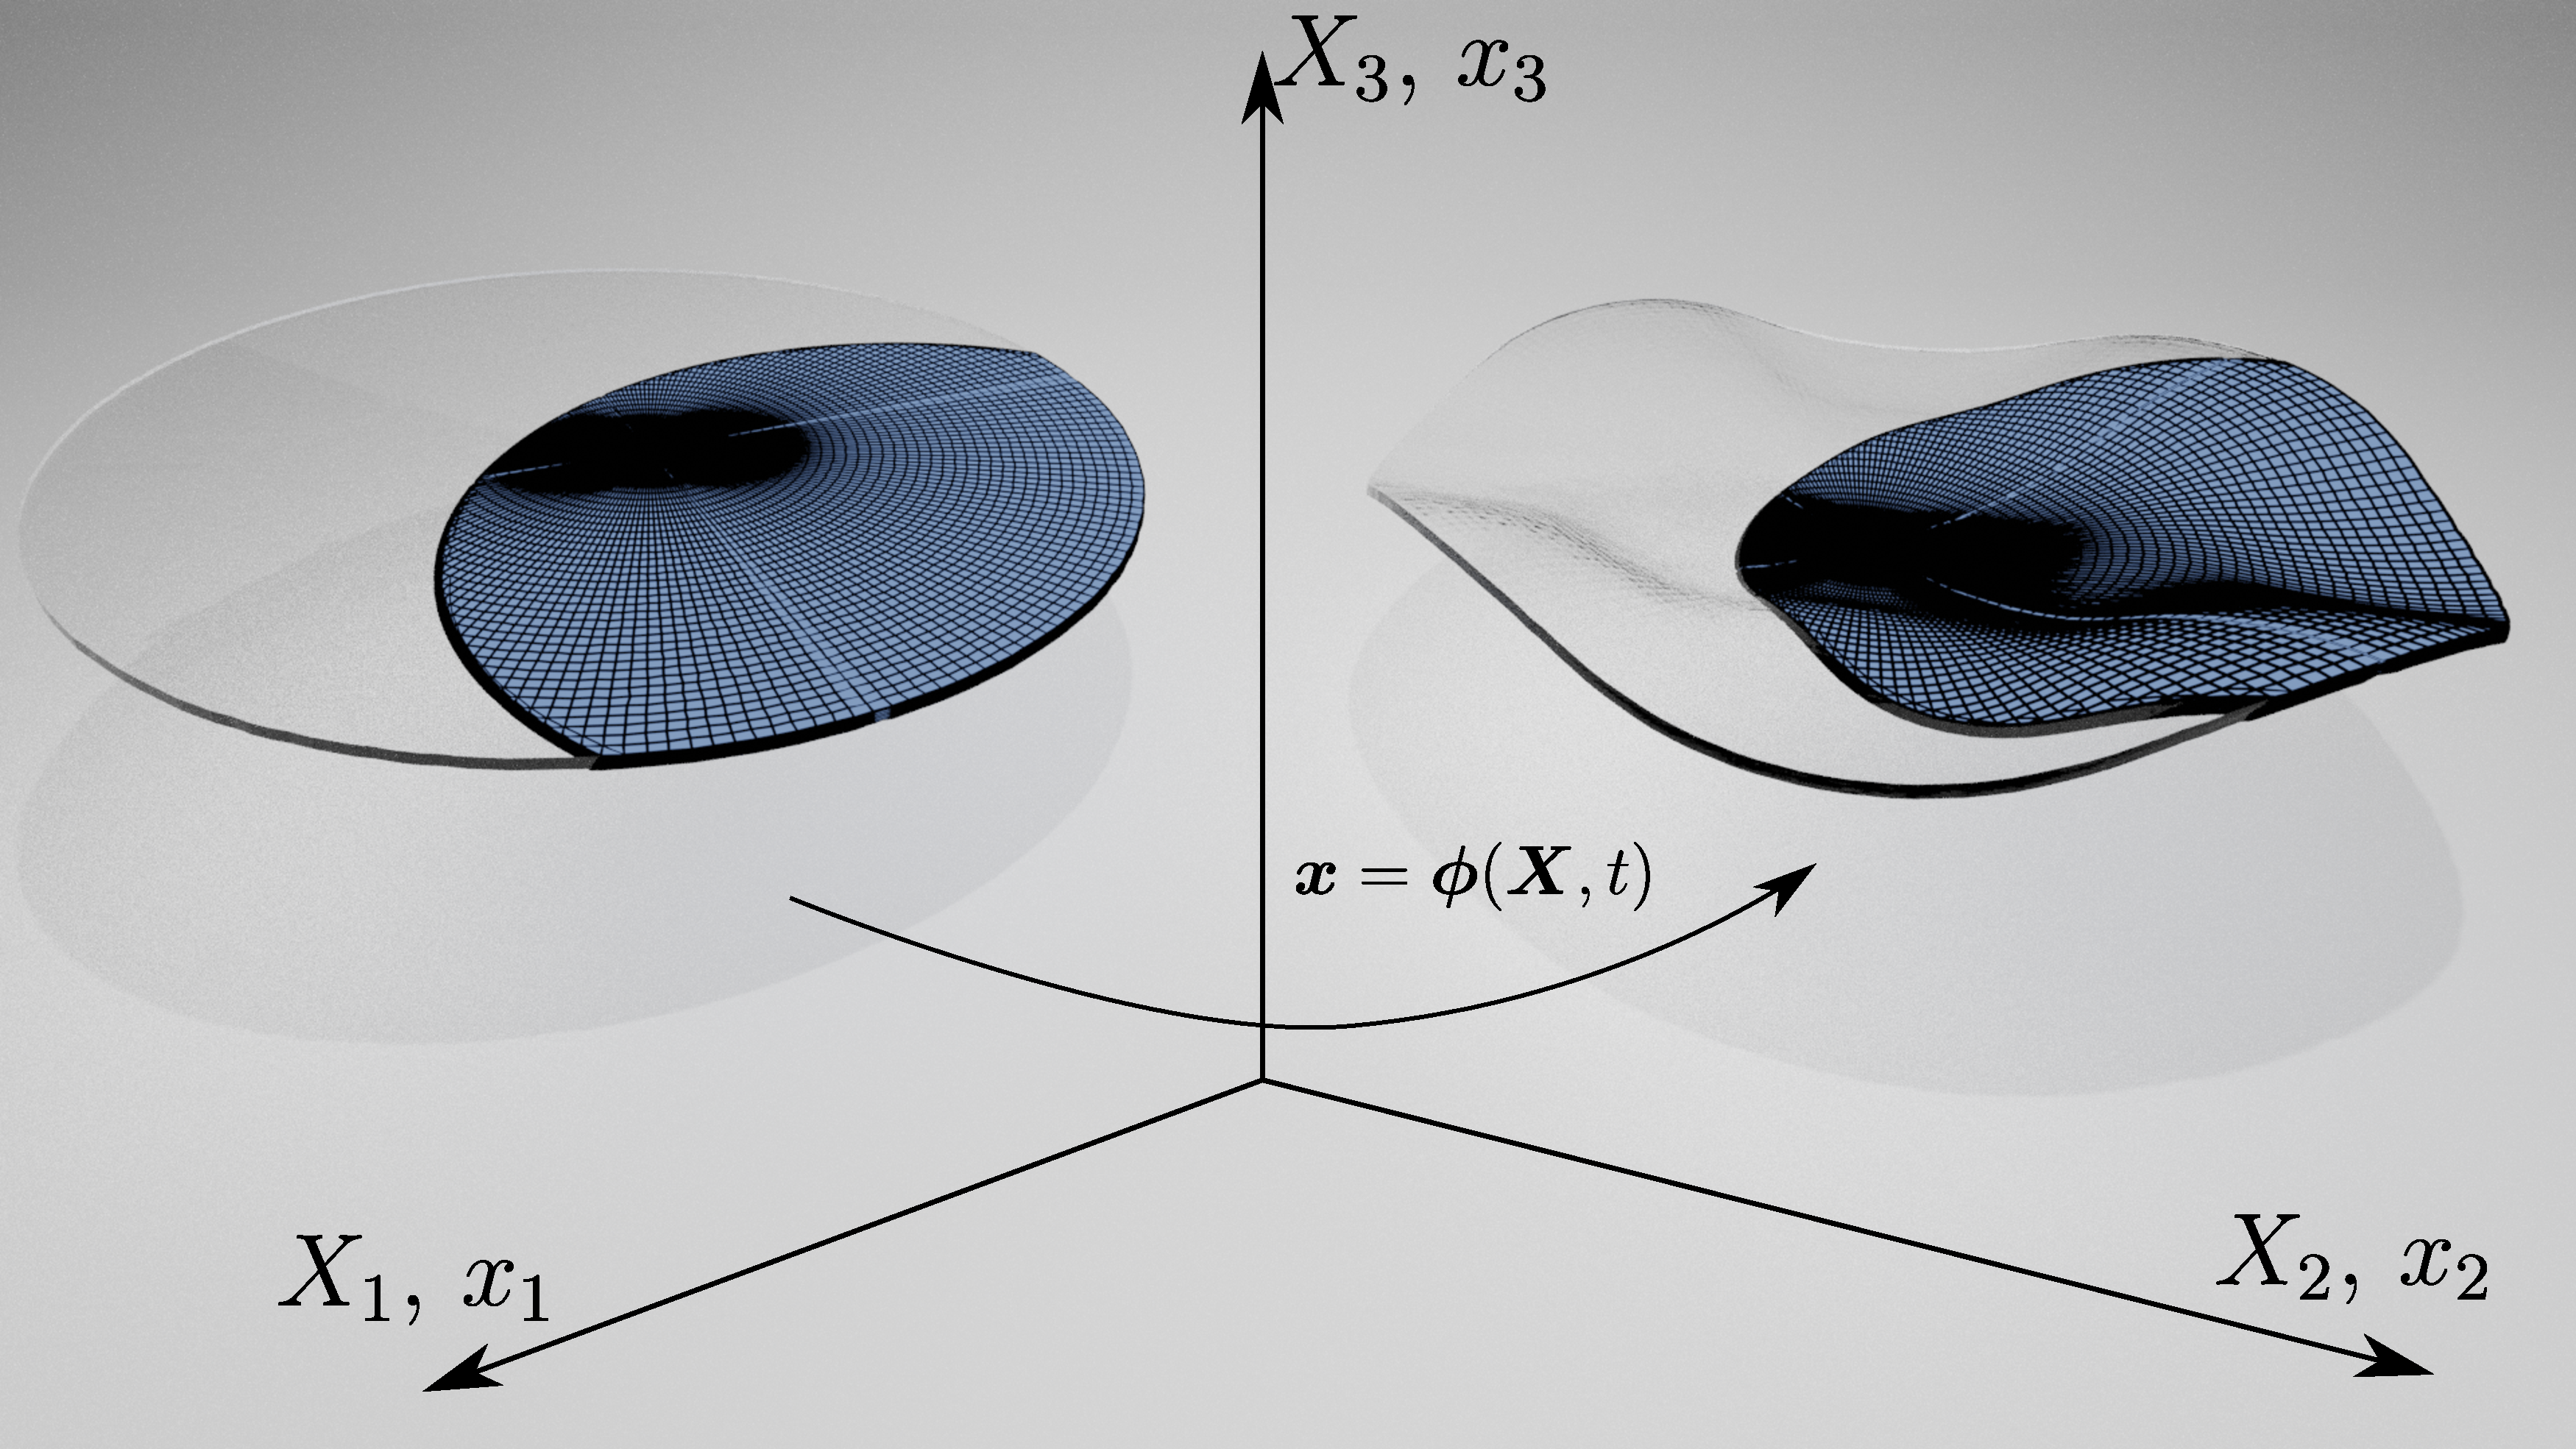
\includegraphics[width=0.6\textwidth]{Figures/InkScape/TheMappingdeLaOstia}
	\end{center}
	\caption{The mapping $\vect{\phi}$ and the reference $\mathcal{B}_0$ (left) and deformed $\mathcal{B}$ (right) configurations.}
	\label{fig:superpotato}
\end{figure}

% \footnote{In addition, throughout the paper, the symbol $(\cdot)$ is used to indicate the scalar product or contraction of a single index $\vect{a}\cdot \vect{b}=a_i b_i$; the symbol $(:)$ is used to indicate double contraction of two indices $\vect{A}:\vect{B}=A_{ij}B_{ij}$; the symbol $(\times)$ is used to indicate the cross product between vectors $[\vect{a} \times \vect{b}]_i=\mathcal{E}_{ijk}a_jb_k$ and the symbol $(\otimes)$ is used to indicate the outer or dyadic product $[\vect{a}\otimes \vect{b}]_{ij}=a_ib_j$.}. 
%As shown in References \cite{Bonet_cross_product_2016,Bonet_polyconvexity_2015}, the definitions of $\vect{H}$ and $J$ in \eqref{eqn:H and J tensor cross product expression}, although equivalent to those in \eqref{eqn:H and J classical}, are very appealing as they yield simpler expressions for their directional derivatives \cite{Bonet_polyconvexity_2015,Bonet_cross_product_2016, Gil_electro_partI_2016,Gil_electro_partII_2016,Gil_electro_partIII_2016, Betsch_EM_thermo_2017}. 

\subsection{Governing equations in nonlinear thermo-mechanics}\label{sec:governing equations}

The behaviour of the EAP is governed by a system of coupled PDEs. These include the conservation of linear momentum  \cite{Gonzalez_book}, which can be recast in a Lagrangian setting as
%
\begin{equation}\label{eqn:local form conservation of linear momentum}
\begin{aligned}
\rho_0\dot{\vect{v}} - \text{DIV}\vect{P} - \vect{f}_0& = \vect{0};&\qquad &\text{in}\,\,\mathcal{B}_0\times [0,T];\\
%
\vect{P}\vect{N}& = \vect{t}_0;&\qquad&\text{on}\,\,\partial_{\boldsymbol{t}}\mathcal{B}_0\times [0,T];\\
%
\vect{\phi} &= \bar{\vect{\phi}};&\qquad & \text{on}\,\,\partial_{\vect{\phi}}\mathcal{B}_0\times [0,T];\\
%
\left.{\vect{\phi}}\right\vert_{t=0}&=\bar{\vect{\phi}}_0;&\qquad
&\text{in}\,\,\mathcal{B}_0;\\
%
\left.\dot{\vect{\phi}}\right\vert_{t=0}&={\bar{\vect{v}}}_0;&\qquad &\text{in}\,\,\mathcal{B}_0,
%#
%
\end{aligned}
\end{equation}
%
where $\rho_0: \mathcal{B}_0\rightarrow \mathbb{R}^{+}$ represents the mass density of the continuum in the reference configuration, $\vect{v}$ the velocity field.
Furthermore, $\vect{f}_0$ represents a body force per unit undeformed volume $\mathcal{B}_0$ and $\vect{t}_0$, the traction force per unit undeformed area applied on $\partial_{\boldsymbol{t}}\mathcal{B}_0\subset \partial \mathcal{B}_0$, such that $\partial_{\boldsymbol{t}}\mathcal{B}_0 \cup \partial_{\vect{\phi}}\mathcal{B}_0 = \partial\mathcal{B}_0$ and $\partial_{\boldsymbol{t}}\mathcal{B}_0 \cap \partial_{\vect{\phi}}\mathcal{B}_0 = \emptyset$. Moreover, $\bar{\vect{\phi}}$ represents the Dirichlet condition for $\vect{\phi}$, $\bar{\vect{\phi}}_0$ and ${\bar{\vect{v}}}_0$ are the initial conditions for the mapping $\vect{\phi}$ and the velocity fields, respectively.
Finally,  local conservation of angular momentum leads to the well-known tensor condition $\vect{F P} = \vect{P}^T\vect{F}^T$, where $\vect{P}$ represents the first Piola-Kirchhoff stress tensor. 
%

The second set of PDEs that govern the behaviour of the EAP comprises the electrostatic form of the Gauss' and Faraday's laws, recast in a Lagrangian setting as follows
%
\begin{equation}\label{eqn:local form Gauss Faraday}
\begin{aligned}
\vect{E}_0& = -\partial_{\vect{X}}\varphi;&\qquad &\text{in}\,\,\mathcal{B}_0\times [0,T];\\
%
\text{DIV}\vect{D}_0 & = -\rho^e_0;&\qquad &\text{in}\,\,\mathcal{B}_0\times [0,T];\\
%
\vect{D}_0\cdot\vect{N}& = -{\omega}^e_0;&\qquad&\text{on}\,\,\partial_{\omega}\mathcal{B}_0\times [0,T];\\
%
{\varphi} &= \bar{{\varphi}};&\qquad & \text{on}\,\,\partial_{{\varphi}}\mathcal{B}_0\times [0,T],
%
\end{aligned}
\end{equation}
%
where $\varphi : \mathcal{B}_0\rightarrow \mathbb{R}$ represents the electric potential, 
 $\rho^e_0: \mathcal{B}_0\rightarrow \mathbb{R}$ is the electric charge per unit volume in the reference configuration 
 and $\omega_0$, the electric charge per unit undeformed area applied on $\partial_{\omega}\mathcal{B}_0\subset \partial \mathcal{B}_0$, such that $\partial_{\omega}\mathcal{B}_0 \cup \partial_{{\varphi}}\mathcal{B}_0 = \partial\mathcal{B}_0$ and $\partial_{\omega}\mathcal{B}_0 \cap \partial_{{\varphi}}\mathcal{B}_0 = \emptyset$. Finally, $\bar{{\varphi}}$ represents the Dirichlet condition for ${\varphi}$. In above equation \eqref{eqn:local form Gauss Faraday}, $\vect{E}_0$ and $\vect{D}_0$ represent the material electric field and electric displacement field, respectively.

Finally, the last coupled PDE governing the behaviour of the EAP is the balance of energy, which in the absence of internal state variables (i.e. plastic strain or viscoelasticity), can be written in a Lagrangian setting as
%
\begin{equation}\label{eqn:local form energy}
\begin{aligned}
\theta\dot{\eta} + \text{DIV}\vect{Q} - R_{\theta} & = 0;&\qquad& \text{in}\,\,\mathcal{B}_0\times [0,T];\\
%
\vect{Q}\cdot\vect{N}& = -Q_{\theta};&\qquad&\text{on}\,\, \partial_{Q}\mathcal{B}_0\times [0,T];\\
%
\theta & = \bar{\theta};&\qquad&\text{on}\,\,\partial_{\theta}\mathcal{B}_0\times [0,T];\\
%%#
\left.{\theta}\right\vert_{t=0}&={\bar{\theta}}_0;&\qquad& \text{in}\,\,\mathcal{B}_0,
\end{aligned}
\end{equation}
%
where $\theta$ is the absolute temperature field and $\eta$ and $\vect{Q}$, the entropy and heat flux per unit undeformed volume $\mathcal{B}_0$, respectively. In addition, $R_{\theta}$  represents the heat source per unit undeformed volume $\mathcal{B}_0$ and $Q_{\theta}$, the heat source per unit undeformed area applied on $\partial_{Q}\mathcal{B}_0\subset\partial\mathcal{B}_0$. In \eqref{eqn:local form energy}, $\partial_{\theta}\mathcal{B}_0$ represents the part of the boundary $\partial\mathcal{B}_0$ where essential temperature boundary conditions are applied such that $\partial_{Q}\mathcal{B}_0\cup\partial_{\theta}\mathcal{B}_0 = \partial\mathcal{B}_0$ and $\partial_{Q}\mathcal{B}_0\cap\partial_{\theta}\mathcal{B}_0 = \emptyset$. 
%


\section{Constitutive equations in nonlinear thermo-electro-elasticity}\label{sec:constitutive equations}
%The governing equations presented in Section \ref{sec:nonlinear continuum electromechanics} are coupled by means of a suitable constitutive law. 
The objective of the following section is to introduce some notions on  constitutive laws in thermo-electro-elasticity. 

\subsection{The Helmholtz free energy}\label{sec:helmholtz}

%\begin{equation}
%\begin{aligned}
%D\vect{F}[\delta\vect{x}] & = \vect{\nabla}_0\delta\vect{x};&\quad
%D^2\vect{F}[\delta\vect{x};\Delta\vect{x}] & = \vect{0};\\
%%
%D\vect{H}[\delta\vect{x}] & = \vect{F}\Cross D\vect{F}[\delta\vect{x}];&\quad
%D^2\vect{H}[\delta\vect{x};\Delta\vect{x}] & =  D\vect{F}[\delta\vect{x}]\Cross D\vect{F}[\Delta\vect{x}];\\
%%
%DJ[\delta\vect{x}] & = \vect{H}:D\vect{F}[\delta\vect{x}];&\quad
%D^2J[\delta\vect{x};\Delta\vect{x}] & = \vect{F}:\left(D\vect{F}[\delta\vect{x}]\Cross D\vect{F}[\Delta\vect{x}]\right).
%\end{aligned}
%\end{equation}


In the case of thermo-electro-elasticity, and in the absence of internal state variables, the Helmholtz free energy $\Psi$ per unit of undeformed volume can be defined as
%
%
\begin{equation}\label{eqn:definition of CMV}
\Psi:\text{GL}^{+}(3)\times \mathbb{R}^3\times \mathbb{R}^+,\qquad \left(\vect{F},\vect{E}_0,\theta\right)\rightarrow \Psi\left(\vect{F},\vect{E}_0,\theta\right)
\end{equation}
%

In order to derive constitutive equations, we begin with the Clausius-Duhen inequality, which takes the following form
%
\begin{equation}\label{eqn:Clausius-Duhen}
-\dot{\Psi} + \vect{P}:\dot{\vect{F}} - \vect{D}_0\cdot \dot{\vect{E}}_0 - \eta \dot{\theta} - \frac{1}{\theta}\vect{Q}\cdot \partial_{\vect{X}}\theta \geq 0
\end{equation}


For the EAP, following \cite{XXX}, use of the Coleman-Noll procedure into \eqref{eqn:Clausius-Duhen}
%
\begin{equation}
\begin{aligned}
\Big(\vect{P} - \partial_{F}\Psi\Big):\dot{\vect{F}} - \Big(\vect{D}_0 + \partial_{\vect{E}_0}\Psi\Big)\cdot \dot{\vect{E}}_0 - \Big(\eta + \partial_{\theta}\Psi\Big) \dot{\theta} - \frac{1}{\theta}\vect{Q}\cdot \partial_{\vect{X}}\theta \geq 0
\end{aligned}	
\end{equation}


Fourier law relates the spatial heat flux $\vect{q}$ and the spatial gradient of $\theta$ by virtue of the following expression
%
\begin{equation}\label{eqn:Duhamel}
\vect{q} = -\vect{k}\partial_{\vect{x}}\theta,
\end{equation}
%
where $\vect{k}$ represents the semi-positive definite second order thermal conductivity tensor in the deformed configuration. The relation between $\vect{q}$ and its material counterpart $\vect{Q}$ in \eqref{eqn:local form energy} can be carried out by making use of the Gauss' theorem and the Nanson's rule (i.e. $d\vect{a}=\vect{H}d\vect{A}$), yielding \cite{XXX}
%
\begin{equation}
\vect{Q} = -\vect{K}\partial_{\vect{X}}\theta;\qquad
\vect{K} = J^{-1}\vect{H}^T\vect{k}\vect{H}.
\end{equation}

Positive definiteness of the material thermal conductivity tensor $\vect{K}$ permits to establish \cite{Gonzalez_book, Gurtin} the following relationships
%
\begin{equation}\label{eqn:first derivatives Hewlmholtz}
\begin{aligned}
\vect{P} = \partial_{F}\Psi(\vect{F},\vect{E}_0,\theta);\qquad  \vect{D}_0 = -\partial_{\vect{E}_0}\Psi(\vect{F},\vect{E}_0,\theta);\qquad  \eta = -\partial_{\theta}\Psi(\vect{F},\vect{E}_0,\theta).
\end{aligned}	
\end{equation}

The Helmholtz free energy density must adhere to the principle of objectivity or material frame indifference, which entails its invariance with repsect to rotations $\vect{Q}\in \text{SO}(3)$ applied to the spatial configuration, namely
%
\begin{equation}\label{eqn:frame indifference}
	\Psi(\vect{Q}\vect{F}, \vect{E}_0, \theta) = \Psi(\vect{F},\vect{E}_0, \theta);\qquad \forall \vect{F}\in \text{GL}^{+}(3),\, \vect{E}_0 \in \mathbb{R}^3,\, \theta \in \mathbb{R}^{+}, \,\vect{Q}\in \text{SO}(3).
\end{equation}

Furthermore, a second invariance condition must hold, known as the material symmetry conditions, which reads as follows
%
\begin{equation}\label{eqn:material symmetry}
	\Psi(\vect{F}\vect{Q}^T,\vect{Q}\vect{E}_0,\theta) = \Psi(\vect{F},\vect{E}_0,\theta);\qquad \forall \vect{F}\in \text{GL}^{+}(3),\, \vect{E}_0 \in \mathbb{R}^3,\,\theta \in \mathbb{R}^{+}, \,\vect{Q}\in \mathcal{G}\subset \text{O}(3),
\end{equation}
%
where $\mathcal{G}$ denotes the symmetry group of the material under consideration.  Section \ref{subsec:InvariantFormulation} will demonstrate how the two physical conditions specified in equation \eqref{eqn:frame indifference} and \eqref{eqn:material symmetry} can be imposed a priori. 
 Moreover, the Helmholtz free energy density $\Psi(\vect{F},\vect{E}_0,\theta)$, along with the first Piola-Kirchhoff stress tensor $\vect{P}(\vect{F},\vect{E}_0,\theta)$, the electric displacement field $\vect{D}_0(\vect{F},\vect{E}_0,\theta)$ and the entropy $\eta(\vect{F},\vect{E}_0,\theta)$ must vanish in the absence of deformations (i.e. $\vect{F}=\vect{I}$, with $\vect{I}$ the second order identity tensor), electric fields (i.e. $\vect{E}_0=\vect{0}$) and when the temperature is equal to the so-called reference temperature, denoted as $\theta_R$. All that is mathematically stated as
%
\begin{equation}\label{eqn:reference conditions}
\begin{aligned}	
\left.\Psi(\vect{F},\vect{E}_0,\theta)\right\vert_{\vect{I},\vect{0},\theta_R}&=0; &\qquad \left.\vect{P}(\vect{F},\vect{E}_0,\theta)\right\vert_{\vect{I},\vect{0},\theta_R}&:=\left.\partial_{\vect{F}}\Psi(\vect{F},\vect{E}_0,\theta)\right\vert_{\vect{I},\vect{0},\theta_R}=\vect{0}\\
%
\left.\vect{D}_0(\vect{F},\vect{E}_0,\theta)\right\vert_{\vect{I},\vect{0},\theta_R}&=:\left.\partial_{\vect{E}_0}\Psi(\vect{F},\vect{E}_0,\theta)\right\vert_{\vect{I},\vect{0},\theta_R}=\vect{0}; &\qquad \left.\eta(\vect{F},\vect{E}_0,\theta)\right\vert_{\vect{I},\vect{0},\theta_R}&:=\left.\partial_{\theta}\Psi(\vect{F},\vect{E}_0,\theta)\right\vert_{\vect{I},\vect{0},\theta_R}={0}
\end{aligned}	
\end{equation}

Equation \eqref{eqn:first derivatives Hewlmholtz} establishes the relationship between the first derivatives of the Helmholtz free energy density, namely $\{\vect{P},\vect{D}_0,\eta\}$, with their work conjugates, namely $\{\vect{F},\vect{E}_0,\theta\}$, thus closing the system of coupled PDEs in \eqref{sec:governing equations}, governing the behaviour of EAPs. However, the second derivatives of the Helmholtz energy lead also to constitutive tensors with insightful physical relevance, in particular when characterizing the behaviour of the EAP in the linearized regime, i.e. in the vicinity of $\vect{F}\approx \vect{I}$, . These can be encompassed within the (symmetric) Hessian of the Helmholtz free energy density, denoted as $[\mathbb{H}_{\Psi}]$, namely
%
\begin{equation}
[\mathbb{H}_{\Psi}]=\begin{bmatrix}
\partial^2_{\vect{F}\vect{F}}\Psi  &  \partial^2_{\vect{F}\vect{E}_0}\Psi  &  \partial^2_{\vect{F}\theta}\Psi\\
%
  &  \partial^2_{\vect{E}_0\vect{E}_0}\Psi  &  \partial^2_{\vect{F}\theta}\Psi\\
%
\text{sym.}  &    &  \partial^2_{\theta\theta}\Psi
\end{bmatrix}
\end{equation}
%
where $\partial^2_{\vect{F}\vect{F}}\Psi$ represents the fourth order elasticity tensor, $\partial^2_{\vect{F}\vect{E}_0}\Psi$ the third order piezoelectric tensor, $\partial^2_{\vect{E}_0\vect{E}_0}\Psi$ represents the second order dielectric tensor, whereas $\partial^2_{\vect{F}\theta}\Psi$ and $\partial^2_{\vect{E}_0\theta}\Psi$ are second and first order tensors encoding the influence of the thermal field $\theta$ on the first Piola-Kirchhoff stress tensor $\vect{P}$ and on the electric displacement field $\vect{D}_0$. Finally, $\partial^2_{\theta\theta}\Psi$ can be related with a relevant physical property of a material, in particular, the specific heat capacity, denoted as $c_v$, and defined as \cite{Vertechhy}
%
\begin{equation}\label{eqn:heat capacity}
c_v(\vect{F},\vect{E}_0,\theta) = -\theta \partial^2_{\theta\theta}\Psi(\vect{F},\vect{E}_0,\theta)
\end{equation}

In addition to the physical conditions encompassing the objectivity condition \eqref{eqn:frame indifference}, the material symmetry condition \eqref{eqn:material symmetry} and the reference conditions \eqref{eqn:reference conditions}, there are mathematical conditions that the Helmholtz free energy density $\Psi(\vect{F},\vect{E}_0,\theta)$ must comply with. In the context of thermo-electro-elasticity, it is accepted that  suitable conditions that $\Psi(\vect{F},\vect{E}_0,\theta)$ must satisfy are: rank-one convexity with respect to the deformation gradient $\vect{F}$, concavity with respect to $\vect{E}_0$, and concavity with respect to the absolute temperature $\theta$, i.e.
%
\begin{equation}\label{eqn:rank one convexity}
\left(\vect{u}\otimes\vect{V}\right):\partial^2_{\vect{F}\vect{F}}\Psi:\left(\vect{u}\otimes\vect{V}\right)\geq 0;\qquad
%
%
%
\begin{bmatrix}
\vect{V}\\
\delta\theta 
\end{bmatrix}: \begin{bmatrix}
\partial^2_{\vect{E}_0\vect{E}_0}\Psi  &  \partial^2_{\vect{E}_0\theta}\Psi\\
%
\text{sym.}  &  \partial^2_{\theta\theta}\Psi
\end{bmatrix}\, \begin{bmatrix}
\vect{V}\\
\delta\theta 
\end{bmatrix}\leq 0,
%
\end{equation}
%
which must hold for $\forall \vect{u},\vect{V}\in \mathbb{R}^{3},\,\delta\theta\in\mathbb{R}^{+}, \,\,\{\vect{F},\vect{E}_0,\theta\}\in\{\text{GL}^{+}(3),\mathbb{R}^3,\mathbb{R}^{+}\}$. Notice that concavity with respect to $\theta$ in \eqref{eqn:rank one convexity} entails positiveness of the specific heat capacity $c_v$ in \eqref{eqn:heat capacity}, whereas the two previous conditions in \eqref{eqn:rank one convexity} are related with the concept of material stability and hyperbolicity in the isothermal case \cite{XX}.


\subsection{Alternative thermodynamical potentials}\label{sec:alternative potentials}

Provided that the Helmholtz free energy density $\Psi(\vect{F},\vect{E}_0,\theta)$ is concave with respect to $\vect{E}_0$ and $\theta$ (as specified by the second and third conditions in \eqref{eqn:rank one convexity}), it becomes possible to define the following three alternative thermodynamic potentials via appropriate Legendre transformations
%
\begin{equation}\label{eqn:other potentials}
\begin{aligned}
e(\vect{F},\vect{D}_0,\eta) & =  \inf_{\vect{E}_0,\theta}\left\{\Psi(\vect{F},\vect{E}_0,\theta) + \vect{E}_0\cdot\vect{D}_0 + \theta \eta \right\}\\
%
\Upsilon(\vect{F},\vect{D}_0,\theta) & =  \inf_{\vect{E}_0}\left\{\Psi(\vect{F},\vect{E}_0,\theta) + \vect{E}_0\cdot\vect{D}_0\right\}\\
%
\Gamma(\vect{F},\vect{E}_0,\eta) & =  \inf_{\theta}\left\{\Psi(\vect{F},\vect{E}_0,\theta) + \theta \eta \right\},
\end{aligned}	
\end{equation}
%
which permits to establish analogous relationships to those in \eqref{eqn:first derivatives Hewlmholtz} as
%
\begin{equation}\label{eqn:piola alternative}
\begin{aligned}
\vect{P}& = \partial_{F}e(\vect{F},\vect{D}_0,\eta);&\qquad  \vect{E}_0& = \partial_{\vect{D}_0}e(\vect{F},\vect{D}_0,\eta);&\qquad  \theta &= \partial_{\eta}e(\vect{F},\vect{D}_0,\eta);\\
%
%
\vect{P} &= \partial_{F}\Upsilon(\vect{F},\vect{D}_0,\theta);&\qquad  \vect{E}_0 &= \partial_{\vect{D}_0}\Upsilon(\vect{F},\vect{D}_0,\theta);&\qquad  \eta &= -\partial_{\theta}\Upsilon(\vect{F},\vect{D}_0,\theta);\\
%
%
\vect{P} &= \partial_{F}\Gamma(\vect{F},\vect{E}_0,\eta);&\qquad  \vect{D}_0& = -\partial_{\vect{E}_0}\Gamma(\vect{F},\vect{E}_0,\eta);&\qquad  \theta& = \partial_{\eta}\Gamma(\vect{F},\vect{E}_0,\eta).
\end{aligned}	
\end{equation} 


Obviously, the three new potentials, $e(\vect{F},\vect{D}_0,\eta)$, $\Upsilon(\vect{F},\vect{D}_0,\theta)$ and $\Gamma(\vect{F},\vect{D}_0,\eta)$ need to comply with the 
material frame indifference condition in \eqref{eqn:frame indifference} and with the material symmetry condition in \eqref{eqn:material symmetry}. Additionally, in the reference configuration, each of these potentials must comply with the conditions below
%
\begin{equation}\label{eqn:reference conditions for the different potentials}
\begin{aligned}
&\left\{\begin{aligned}	
\left.e(\vect{F},\vect{D}_0,\eta)\right\vert_{\vect{I},\vect{0},0}&=0; &\quad \left.{\vect{P}}(\vect{F},\vect{D}_0,\eta)\right\vert_{\vect{I},\vect{0},0}&:=\left.\partial_{\vect{F}}e(\vect{F},\vect{D}_0,\eta)\right\vert_{\vect{I},\vect{0},0}=\vect{0}\\
%
\left.{\vect{E}_0}(\vect{F},\vect{D}_0,\eta)\right\vert_{\vect{I},\vect{0},0}&:=\left.\partial_{\vect{D}_0}e(\vect{F},\vect{D}_0,\eta)\right\vert_{\vect{I},\vect{0},0}=\vect{0}; &\quad \left.\theta(\vect{F},\vect{D}_0,\eta)\right\vert_{\vect{I},\vect{0},0}&:=\left.\partial_{\eta}e(\vect{F},\vect{D}_0,\eta)\right\vert_{\vect{I},\vect{0},0}=\theta_R
\end{aligned}	\right.\\
%
%
&\left\{\begin{aligned}	
\left.\Upsilon(\vect{F},\vect{D}_0,\theta)\right\vert_{\vect{I},\vect{0},\theta_R}&=0; &\quad \left.{\vect{P}}(\vect{F},\vect{D}_0,\theta)\right\vert_{\vect{I},\vect{0},\theta_R}&:=\left.\partial_{\vect{F}}\Upsilon(\vect{F},\vect{D}_0,\theta)\right\vert_{\vect{I},\vect{0},\theta_R}=\vect{0}\\
%
\left.{\vect{E}_0}(\vect{F},\vect{D}_0,\theta)\right\vert_{\vect{I},\vect{0},\theta_R}&:=\left.\partial_{\vect{D}_0}\Upsilon(\vect{F},\vect{D}_0,\theta)\right\vert_{\vect{I},\vect{0},\theta_R}=\vect{0}; &\quad \left.\eta(\vect{F},\vect{D}_0,\theta)\right\vert_{\vect{I},\vect{0},\theta_R}&:=-\left.\partial_{\theta}\Upsilon(\vect{F},\vect{D}_0,\theta)\right\vert_{\vect{I},\vect{0},\theta_R}={0}
\end{aligned}	\right.\\
%
%%
%
&\left\{\begin{aligned}	
\left.\Gamma(\vect{F},\vect{D}_0,\eta)\right\vert_{\vect{I},\vect{0},0}&=0; &\quad \left.{\vect{P}}(\vect{F},\vect{E}_0,\eta)\right\vert_{\vect{I},\vect{0},0}&:=\left.\partial_{\vect{F}}\Gamma(\vect{F},\vect{E}_0,\eta)\right\vert_{\vect{I},\vect{0},0}=\vect{0}\\
%
\left.{\vect{D}_0}(\vect{F},\vect{E}_0,\eta)\right\vert_{\vect{I},\vect{0},0}&:=-\left.\partial_{\vect{D}_0}\Gamma(\vect{F},\vect{E}_0,\eta)\right\vert_{\vect{I},\vect{0},0}=\vect{0}; &\quad \left.\theta(\vect{F},\vect{E}_0,\eta)\right\vert_{\vect{I},\vect{0},0}&:=\left.\partial_{\eta}\Gamma(\vect{F},\vect{E}_0,\eta)\right\vert_{\vect{I},\vect{0},0}=\theta_R
\end{aligned}	\right.\\
%
%
\end{aligned}
\end{equation}



Furthermore, provided that $\Psi(\vect{F},\vect{E}_0,\theta)$ is rank-one convex with respect to $\vect{F}$ (i.e. first condition in \eqref{eqn:rank one convexity}), the resulting thermodynamical potentials in above \eqref{eqn:other potentials} would satisfy the following convexity/concavity properties
%
\begin{equation}\label{eqn:rank one convexity other potentials}
\begin{aligned}
%	
%e(\vect{F},\vect{D}_0,\eta)\Rightarrow 
%
&\begin{bmatrix}
\left(\vect{u}\otimes\vect{V}\right)\\
\vect{V}_{\perp}\\
\delta \eta
\end{bmatrix}:\begin{bmatrix}
\partial^2_{\vect{F}\vect{F}}e  &  \partial^2_{\vect{F}\vect{D}_0}e  &  \partial^2_{\vect{F}\eta}e\\
%
\partial^2_{\vect{F}\vect{F}}e  &  \partial^2_{\vect{F}\vect{D}_0}e  &  \partial^2_{\vect{F}\eta}e\\
%
\partial^2_{\vect{F}\vect{F}}e  &  \partial^2_{\vect{F}\vect{D}_0}e  &  \partial^2_{\vect{F}\eta}e
\end{bmatrix}:\begin{bmatrix}
\left(\vect{u}\otimes\vect{V}\right)\\
\vect{V}_{\perp}\\
\delta \eta
\end{bmatrix}
\geq 0;&\\
%
%
%
%\Upsilon(\vect{F},\vect{D}_0,\theta)\Rightarrow 
%
&\begin{bmatrix}
\left(\vect{u}\otimes\vect{V}\right)\\
\vect{V}_{\perp}
\end{bmatrix}:\begin{bmatrix}
\partial^2_{\vect{F}\vect{F}}\Upsilon  &  \partial^2_{\vect{F}\vect{D}_0}\Upsilon  \\
%
\text{sym.}  &  \partial^2_{\vect{D}_0\vect{D}_0}\Upsilon\\
\end{bmatrix}:\begin{bmatrix}
\left(\vect{u}\otimes\vect{V}\right)\\
\vect{V}_{\perp}
\end{bmatrix}
\geq 0;&\qquad
%
%
&\partial^2_{\theta\theta}\Upsilon\leq 0;\\
%
%
%
%\Gamma(\vect{F},\vect{E}_0,\eta)\Rightarrow 
%
&\begin{bmatrix}
\left(\vect{u}\otimes\vect{V}\right)\\
\delta \eta
\end{bmatrix}:\begin{bmatrix}
\partial^2_{\vect{F}\vect{F}}\Gamma   &  \partial^2_{\vect{F}\eta}\Gamma\\
%
\text{sym.} & \partial^2_{\eta\eta}\Gamma
\end{bmatrix}:\begin{bmatrix}
\left(\vect{u}\otimes\vect{V}\right)\\
\delta \eta
\end{bmatrix}
\geq 0;&\qquad
%
&\vect{V}\cdot \partial^2_{\vect{E}_0\vect{E}_0}\Gamma\, \vect{V}\geq 0,
%
%
\end{aligned}
\end{equation}
%
%
%
%
which must hold for 
%
\begin{equation}
\begin{aligned}
& \vect{u},\vect{V},\vect{V}_{\perp}
\in \mathbb{R}^{3}, \delta\eta\in\mathbb{R},&\quad&\{\vect{F},\vect{D}_0,\eta\}\in\{\text{GL}^{+}(3),\mathbb{R}^3,\mathbb{R}\}	\\
 %
&\vect{u},\vect{V},\vect{V}_{\perp}\in \mathbb{R}^{3},&\quad&\{\vect{F},\vect{D}_0,\theta\}\in\{\text{GL}^{+}(3),\mathbb{R}^3,\mathbb{R}^{+}\}\\
%
&\vect{u},\vect{V}\in \mathbb{R}^{3}, \delta\eta\in\mathbb{R},&\quad&\{\vect{F},\vect{E}_0,\eta\}\in\{\text{GL}^{+}(3),\mathbb{R}^3,\mathbb{R}\},		 
\end{aligned}	
\end{equation}
%
%
respectively, where $\vect{V}_{\perp}$ is such that $\vect{V}_{\perp}\cdot \vect{V}=0$. Above conditions, in conjunction with \eqref{eqn:rank one convexity} dictate that the four potentials, namely $\Psi(\vect{F},\vect{E}_0,\theta)$, $e(\vect{F},\vect{D}_0,\eta)$, $\Upsilon(\vect{F},\vect{D}_0,\theta)$ and $\Gamma(\vect{F},\vect{E}_0,\theta)$, in the vicinity of the reference configuration, namely $\vect{F}\approx \vect{I}$, $\vect{E}_0\approx \vect{0}$ and $\theta\approx \theta_R$, will adopt the convexity/concavity properties displayed in Figure \eqref{fig:convexity}.

\begin{figure}[htpb!]	
	\centering
	\begin{tabular}{cc}
	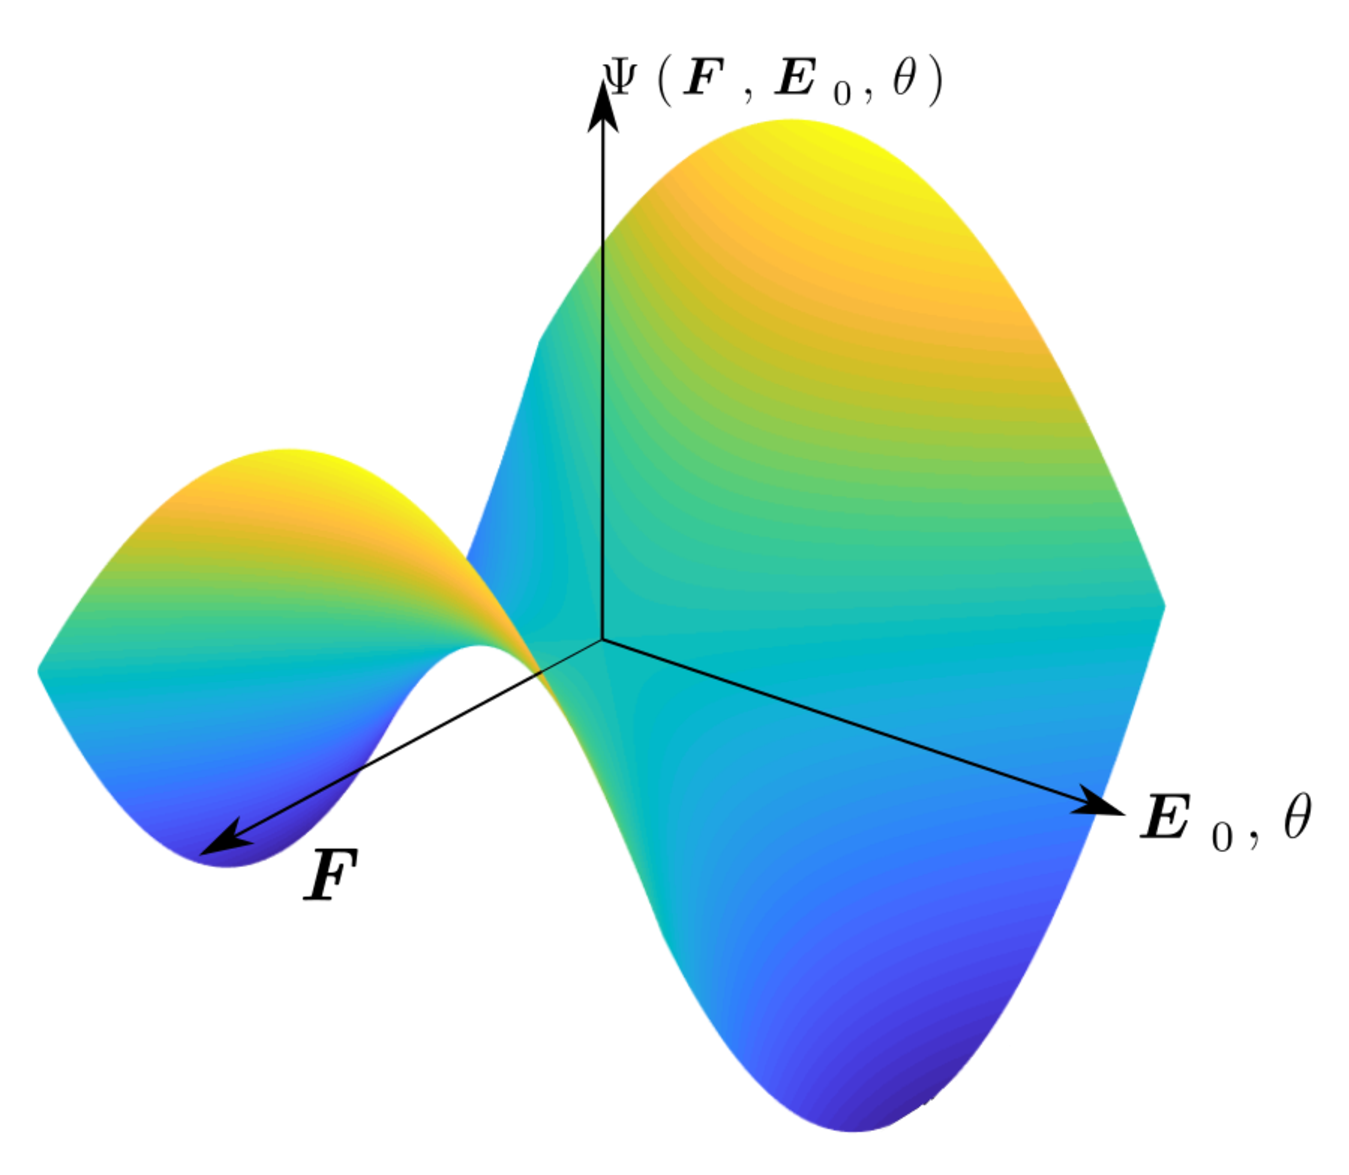
\includegraphics[width=0.35\textwidth]{Figures/InkScape/convexity_psi}&
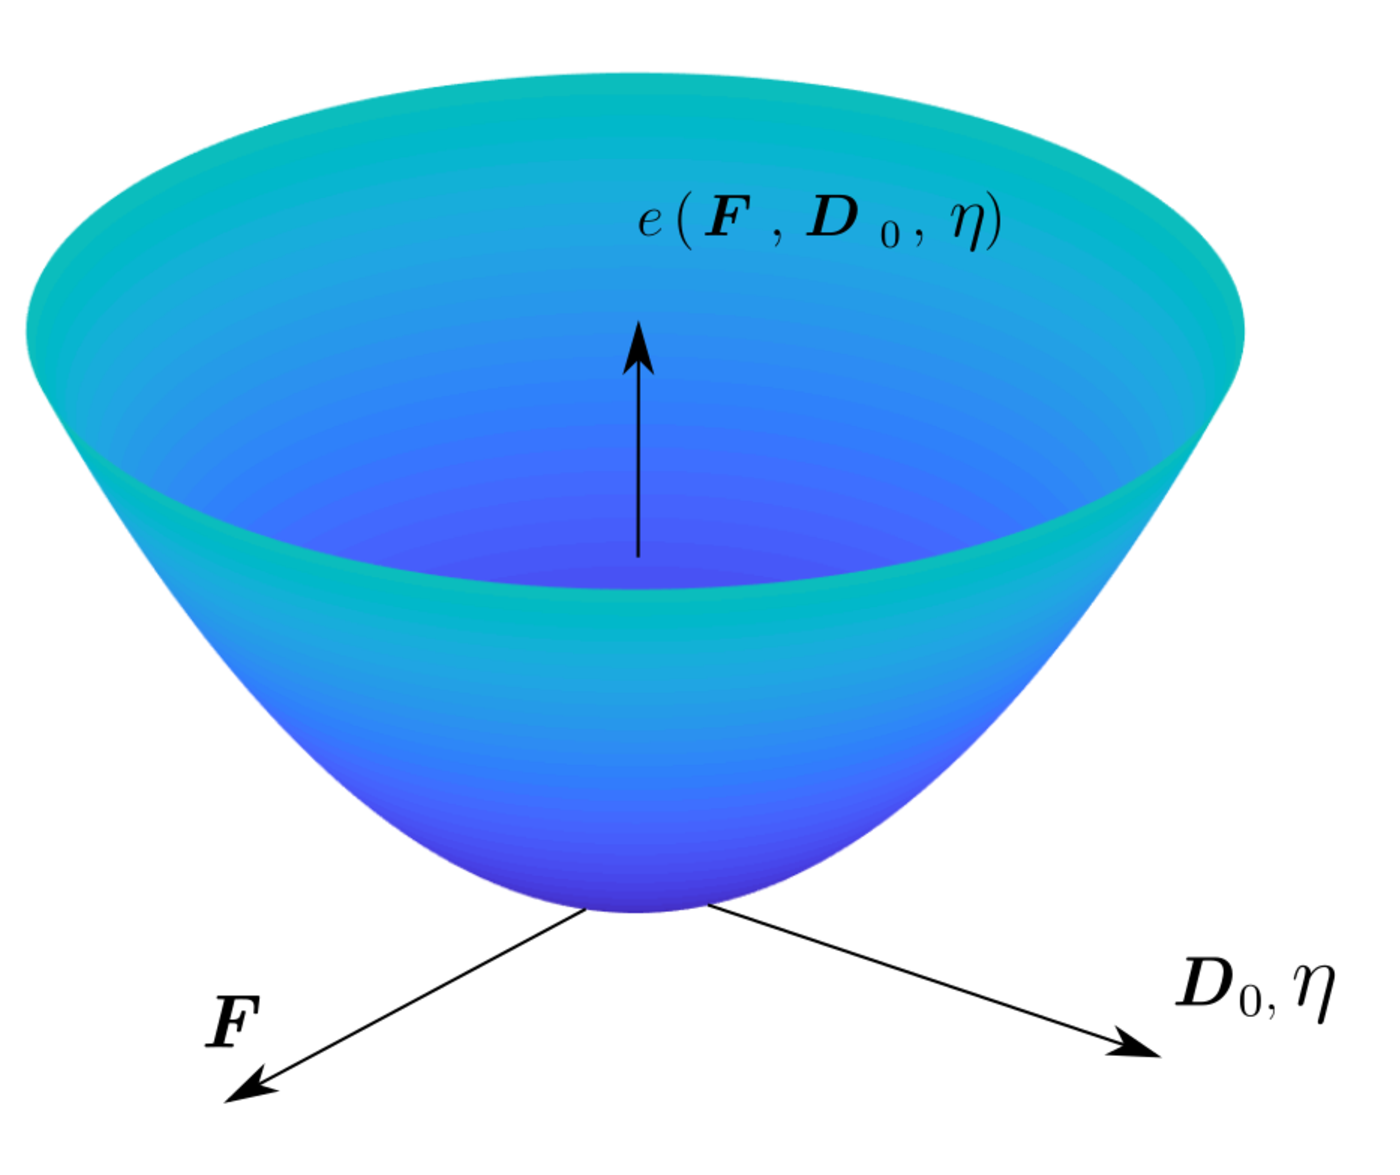
\includegraphics[width=0.35\textwidth]{Figures/InkScape/convexity_e}\\
%
(a)  &  (b)\\
%
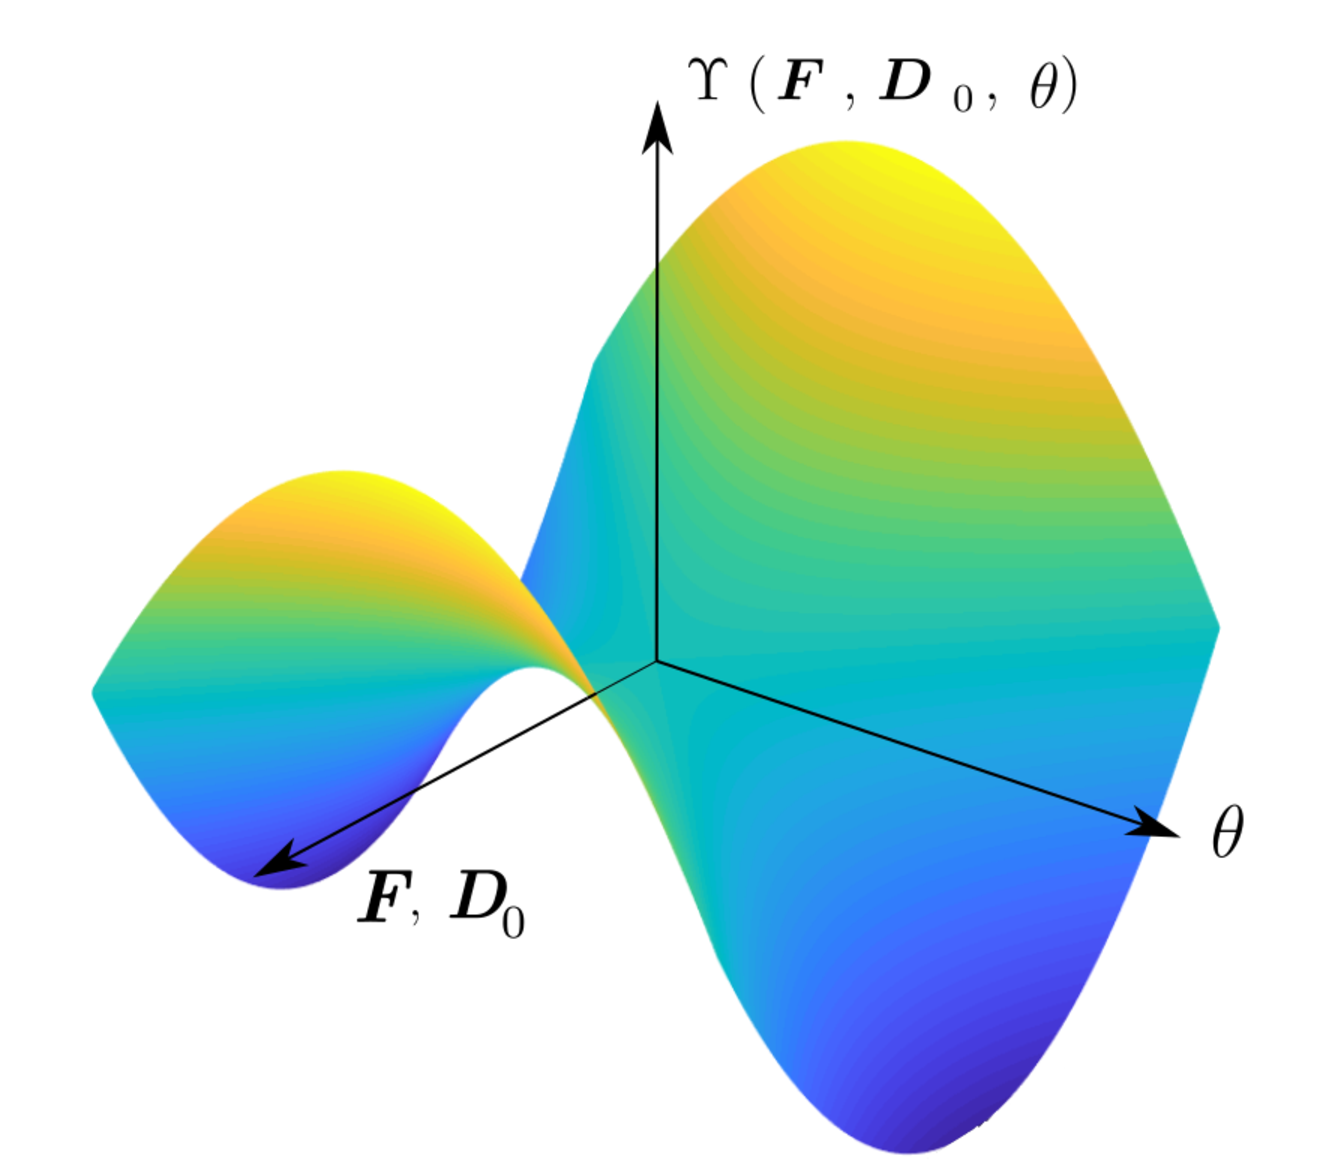
\includegraphics[width=0.35\textwidth]{Figures/InkScape/convexity_upsilon}&
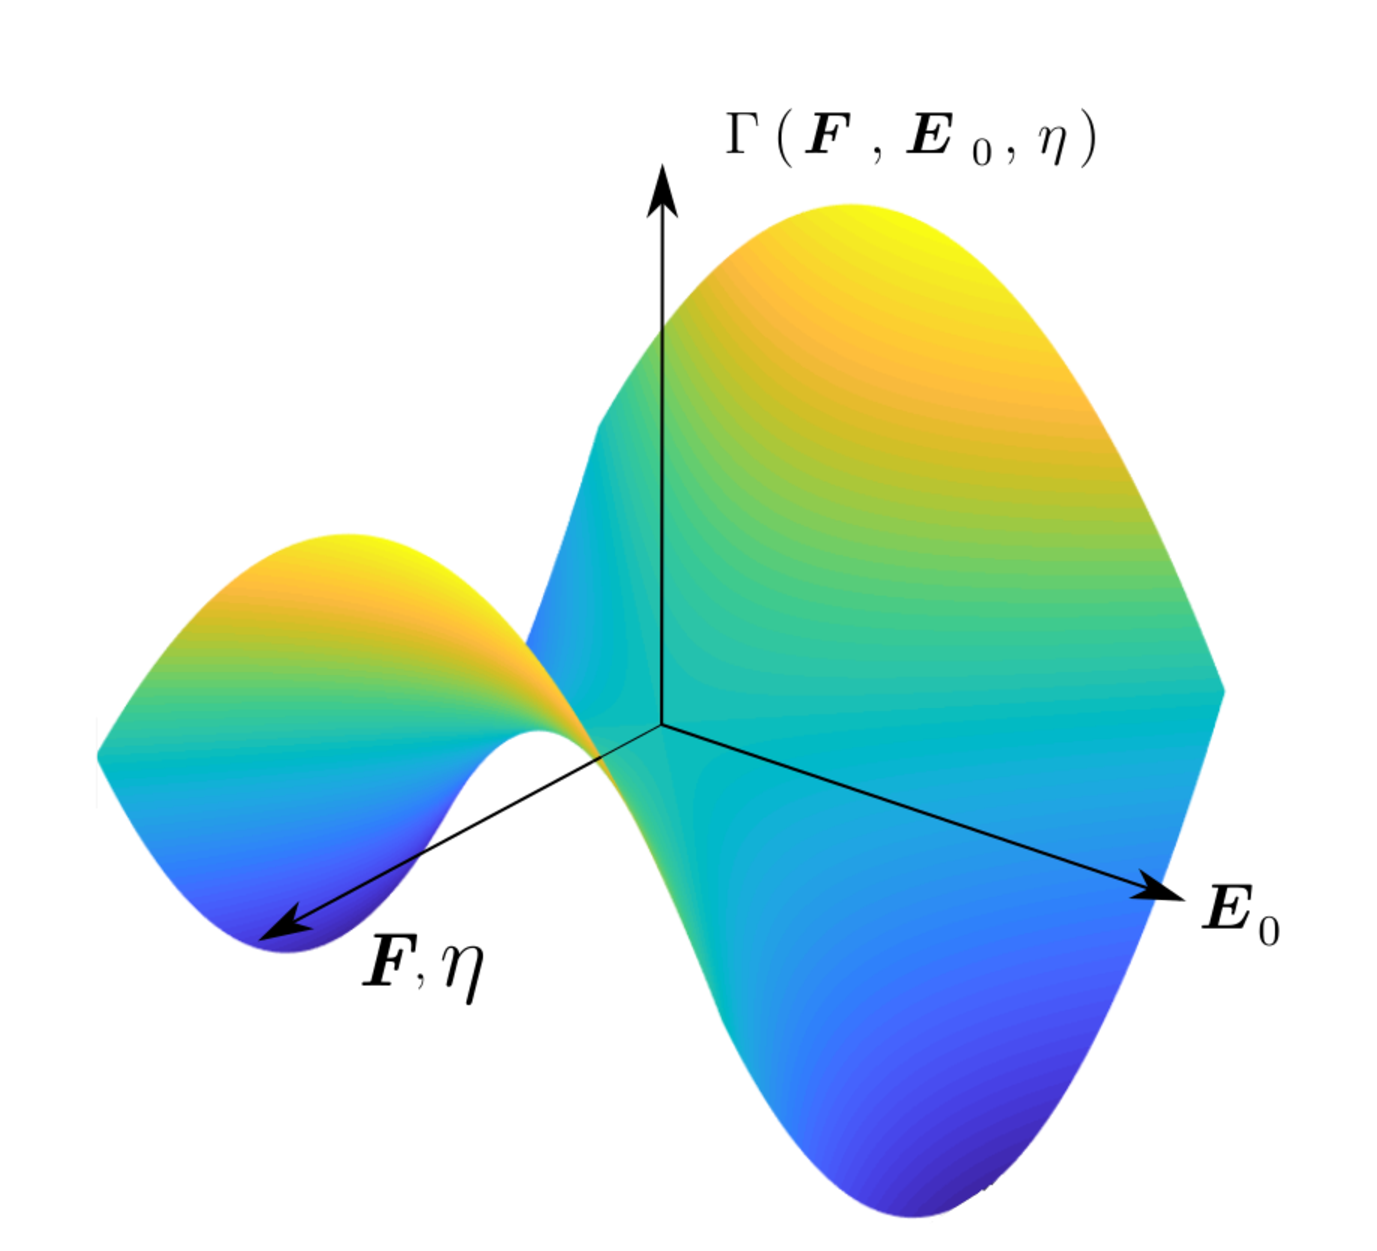
\includegraphics[width=0.35\textwidth]{Figures/InkScape/convexity_gamma}	\\
%	
(c)  &  (d)
	\end{tabular}
	\vspace{-2mm}
	\caption{Convexity/concavity properties of the various thermodynamical potentials $\Psi(\vect{F},\vect{E}_0,\theta)$, $e(\vect{F},\vect{D}_0,\eta)$, $\Upsilon(\vect{F},\vect{D}_0,\theta)$ and $\Gamma(\vect{F},\vect{E}_0,\theta)$ in the vicinity of the reference configuration (i.e. $\vect{F}\approx \vect{I}$, $\vect{E}_0\approx \vect{0}$ and $\theta\approx \theta_R$). Specifically, we observe: $\Psi(\vect{F},\vect{E}_0,\theta)$ is convex with respect to $\vect{F}$ and concave with respect to $\{\vect{E}_0,\theta\}$; $e(\vect{F},\vect{D}_0,\eta)$ is convex with respect to $\{\vect{F},\vect{D}_0,\eta\}$; $\Upsilon(\vect{F},\vect{D}_0,\theta)$ is convex with respect to $\{\vect{F},\vect{D}_0\}$ and concave with respect to $\theta$; $\Gamma(\vect{F},\vect{E}_0,\eta)$ is convex with respect to $\{\vect{F},\eta\}$ and concave with respect to $\vect{E}_0$.}
	\label{fig:convexity}
\end{figure}

 
 
 


As discussed in \cite{XX}, defining phenomenological thermodynamic potentials that must satisfy both rank-one convexity and concavity conditions-such as $\Psi(\vect{F},\vect{E}_0,\theta)$, $\Upsilon(\vect{F},\vect{D}_0,\theta)$, and $\Gamma(\vect{F},\vect{E}_0,\eta)$-is generally more challenging than when the potential is only required to be rank-one convex or convex with respect to all its arguments, as is the case with the internal energy $e(\vect{F},\vect{D}_0,\theta)$. Motivated by this simplification, the authors in \cite{XX} aimed to define constitutive models for the internal energy of EAPs within the framework of isothermal electro-mechanics. This was achieved by extending the concept of polyconvexity, originally from hyperelasticity (purely mechanical systems), to this multi-physics context. Indeed, a sufficient condition for ensuring the rank-one convexity of $e(\vect{F},\vect{D}_0,\eta)$, as shown in equation \eqref{eqn:rank one convexity other potentials}, can be fulfilled through the polyconvexity of $e(\vect{F},\vect{D}_0,\eta)$. For this purpose, we assume the existence of a function $\mathbb{W}$ such that:
%
\begin{equation}
\mathbb{W}:\text{GL}^{+}(3)\times \text{GL}^{+}(3)\times \mathbb{R}^{+}\times \mathbb{R}^3\times \mathbb{R}^3\times \mathbb{R},\qquad (\vect{F},\vect{H},J,\vect{D}_0,\vect{d},\eta)\rightarrow \mathbb{W}(\vect{F},\vect{H},J,\vect{D}_0,\vect{d},\eta)
\end{equation}
%
where $\vect{H}$ and $J$ are the co-factor and determinant of $\vect{F}$, defined in \eqref{eqn:H and J classical} and \eqref{eqn:H and J tensor cross product expression}, whilst $\vect{d}$ is a field obtained as $\vect{d}=\vect{FD}_0$. Then, $e(\vect{F},\vect{D}_0,\eta)$ is said to be polyconvex \cite{Ball_1976,Ball_2002,Ball_Murat_1976} if it can be equivalently written as
%
\begin{equation}\label{eqn:polyconvexity}
e(\vect{F},\vect{D}_0,\eta)=\mathbb{W}(\vect{F},\vect{H},J,\vect{D}_0,\vect{d},\eta)
\end{equation}
%
where $\mathbb{W}(\vect{F},\vect{H},J,\vect{D}_0,\vect{d},\eta)$ must be convex with respect to all its arguments. For twicely differentiable functions, convexity of $\mathbb{W}(\vect{F},\vect{H},J,\vect{D}_0,\vect{d},\eta)$ is equivalent to positive definiteness of its Hessian operator $[\mathbb{H}_{\mathbb{W}}]$, i.e.
%
\begin{equation}
\delta{\mathcal{V}}^T:[\mathbb{H}_{\mathbb{W}}]:\delta{\mathcal{V}}\geq 0,\quad \forall\, \delta\mathcal{V}=\begin{bmatrix}\delta\vect{F} & \delta\vect{H} & \delta J & \delta\vect{D}_0 & \delta\vect{d} & \delta \eta
\end{bmatrix}^T,
\end{equation}
%
where the (symmetric) Hessian operator  $[\mathbb{H}_{\mathbb{W}}]$ incorporates all the second derivatives of $\mathbb{W}$, i.e.
%
\begin{equation}
[\mathbb{H}_{\mathbb{W}}]=\begin{bmatrix}
\partial^2_{\vect{F}\vect{F}}\mathbb{W}  &  
\partial^2_{\vect{F}\vect{H}}\mathbb{W}  &
\partial^2_{\vect{F}J}\mathbb{W}&
\partial^2_{\vect{F}\vect{D}_0}\mathbb{W}&
\partial^2_{\vect{F}\vect{d}}\mathbb{W}&
\partial^2_{\vect{F}\eta}\mathbb{W}\\
%
%
&
\partial^2_{\vect{H}\vect{H}}\mathbb{W}  &
\partial^2_{\vect{H}J}\mathbb{W}&
\partial^2_{\vect{H}\vect{D}_0}\mathbb{W}&
\partial^2_{\vect{H}\vect{d}}\mathbb{W}&
\partial^2_{\vect{H}\eta}\mathbb{W}\\
%
%
& &
\partial^2_{JJ}\mathbb{W}&
\partial^2_{J\vect{D}_0}\mathbb{W}&
\partial^2_{J\vect{d}}\mathbb{W}&
\partial^2_{J\eta}\mathbb{W}\\
%
%
&&&\partial^2_{\vect{D}_0\vect{D}_0}\mathbb{W}&
\partial^2_{\vect{D}_0\vect{d}}\mathbb{W}&
\partial^2_{\vect{D}_0\eta}\mathbb{W}\\
%
%
\text{sym.}&&&&\partial^2_{\vect{d}\vect{d}}\mathbb{W}&
\partial^2_{\vect{d}\eta}\mathbb{W}\\
%
%
&&&&&\partial^2_{\eta\eta}\mathbb{W}
%
\end{bmatrix}
\end{equation}



\subsection{Invariant-based thermo-electro-mechanics}\label{subsec:InvariantFormulation}


A simple manner to accommodate the principle of objectivity or material frame indifference and the requirement of material symmetry is through the dependence of any of the thermodynamical potentials, namely $\Psi(\vect{F},\vect{E}_0,\theta)$, $e(\vect{F},\vect{D}_0,\eta)$, $\Upsilon(\vect{F},\vect{D}_0,\theta)$ or $\Gamma(\vect{F},\vect{E}_0,\eta)$
with respect to invariants of the right Cauchy-Green deformation gradient tensor $\vect{C}=\vect{F}^T\vect{F}$,  $\vect{E}_0$ or $\vect{D}_0$ and also with respect to $\theta$ or $\eta$. Let us denote as  ${\bf I}_{\Psi}$, ${\bf I}_{e}$, ${\bf I}_{\Upsilon}$ and ${\bf I}_{\Gamma}$ the set of electro-mechanical objective invariants of $\Psi(\vect{F},\vect{E}_0,\theta)$, $e(\vect{F},\vect{D}_0,\eta)$, $\Upsilon(\vect{F},\vect{D}_0,\theta)$ or $\Gamma(\vect{F},\vect{E}_0,\eta)$, respectively,  required to characterise a given material symmetry group $\mathcal{G}$. Then, it is possible to express the four thermodynamical potentials equivalently as
%
\begin{equation}\label{eqn:Energy_wrt_Invariants}
\begin{aligned}
% 	U:\mathbb{R}^n\rightarrow \mathbb{R},\qquad (\vect{\mathcal{I}})\mapsto
% U({\bf I}),\qquad 
\Psi(\vect{F},\vect{E}_0,\theta)&=\mathbb{U}_{\Psi}({\bf I}_{\Psi}(\vect{C},\vect{E}_0),\theta);&\qquad
%
e(\vect{F},\vect{D}_0,\eta)&=\mathbb{U}_{e}({\bf I}_{e}(\vect{C},\vect{D}_0),\eta);\\
%
\Upsilon(\vect{F},\vect{D}_0,\theta)&=\mathbb{U}_{\Upsilon}({\bf I}_{\Upsilon}(\vect{C},\vect{D}_0),\theta);&\qquad
%
\Gamma(\vect{F},\vect{E}_0,\eta)&=\mathbb{U}_{\Gamma}({\bf I}_{\Gamma}(\vect{C},\vect{E}_0),\eta).
%
\end{aligned}
\end{equation}

Application of the chain rule into equation \eqref{eqn:first derivatives Hewlmholtz} or \eqref{eqn:piola alternative} permits of obtain the first Piola-Kirchhoff stress tensor $\vect{P}$, $\vect{D}_0$ or $\vect{E}_0$, and $\theta$ or $\eta$ in terms of the derivatives of above invariant-based potentials with respect to their arguments
%
\begin{equation}\label{eqn:Piola invariants isotropy}
\begin{aligned}	
\vect{P}&=\sum_{i=1}^n\Big(\partial_{I_{\Psi_i}}\mathbb{U}_{\Psi}\Big) \partial_{\vect{F}}I_{\Psi_i};&\qquad
%
\vect{D}_0&=-\sum_{i=1}^n\Big(\partial_{I_{\Psi_i}}\mathbb{U}_{\Psi}\Big) \partial_{\vect{E}_0}I_{\Psi_i};&\qquad
%
\eta  & =  -\partial_\theta \mathbb{U}_{\Psi}\\
%
%
\vect{P}&=\sum_{i=1}^n\Big(\partial_{I_{e_i}}\mathbb{U}_e\Big) \partial_{\vect{F}}I_{e_i};&\qquad
%
\vect{E}_0&=\sum_{i=1}^n\Big(\partial_{I_{e_i}}\mathbb{U}_e\Big) \partial_{\vect{D}_0}I_{e_i};&\qquad
%
\theta &  =  \partial_\eta \mathbb{U}_e\\
%
%
\vect{P}&=\sum_{i=1}^n\Big(\partial_{I_{\Upsilon_i}}\mathbb{U}_{\Upsilon}\Big) \partial_{\vect{F}}I_{\Upsilon_i};&\qquad
%
\vect{E}_0&=\sum_{i=1}^n\Big(\partial_{I_{\Upsilon_i}}\mathbb{U}_{\Upsilon}\Big) \partial_{\vect{D}_0}I_{\Upsilon_i};&\qquad
%
\eta &  =  -\partial_\theta \mathbb{U}_{\Upsilon}\\
%
%
\vect{P}&=\sum_{i=1}^n\Big(\partial_{I_{\Psi_i}}\mathbb{U}\Big) \partial_{\vect{F}}I_{\Psi_i};&\qquad
%
\vect{D}_0&=-\sum_{i=1}^n\Big(\partial_{I_{{\Gamma}_i}}\mathbb{U}_{\Gamma}\Big) \partial_{\vect{E}_0}I_{{\Gamma}_i};&\qquad
%
\theta  & =  \partial_\eta \mathbb{U}_{\Gamma}
%
\end{aligned}
\end{equation}

%Furthermore, application of the chain rule over equation \eqref{eqn:elasticity} permits to obtain the elasticity tensor $\vect{\mathcal{C}}$ in terms of the derivatives of $U({\bf I})$ as
%
%\begin{equation}\label{eqn:elasticity invariants}
%	\vect{\mathcal{C}}=\sum_{i=1}^n\sum_{j=1}^n\left(\partial^2_{I_iI_j}U\right)\partial_{\vect{F}}I_i\otimes\partial_{\vect{F}}I_j + \sum_{i=1}^n\left(\partial_{I_i}U\right)\partial^2_{\vect{F}\vect{F}}I_i.
%\end{equation}



\subsubsection{Electro-mechanical invariants for isotropy}

For the case of isotropy, the invariants required to characterise this material symmetry group for the thermodynamical potentials depending on $\vect{E}_0$, namely $\Psi(\vect{F},\vect{E}_0,\theta)$ and $\Gamma(\vect{F},\vect{E}_0,\eta)$, and the first derivatives of the latter with respect to $\vect{F}$ and $\vect{E}_0$ (featuring in the definition of $\vect{P}$ and $\vect{D}_0$ in \eqref{eqn:Piola invariants isotropy}) are
%
\begin{equation}\label{eqn:table isotropy}
\begin{aligned}	
I_{\Psi_1} &:= \vect{F}:\vect{F}=\text{tr}(\vect{C}),\quad   &\partial_{\vect{F}}I_{\Psi_1}&=2\vect{F},\quad   &\partial_{\vect{D}_0}I_{\Psi_1}&=\vect{0}\\
%
I_{\Psi_2} &:= \vect{H}:\vect{H}=\text{tr}(\text{Cof}\vect{C}),\quad   &\partial_{\vect{F}}I_{\Psi_2}&=2\vect{H}\Cross \vect{F},\quad   &\partial_{\vect{E}_0}I_{\Psi_2}&=\vect{0}\\
%
I_{\Psi_3}&:=J = (\text{det}\vect{C})^{1/2},&\quad   \partial_{\vect{F}}I_{\Psi_3}&=\vect{H},\quad   &\partial_{\vect{D}_0}I_{\Psi_3}&=0\\
%
I_{\Psi_4} &:= \vect{E}_0\cdot\vect{E}_0,\quad   &\partial_{\vect{F}}I_{\Psi_4}&=\vect{0},\quad   &\partial_{\vect{E}_0}I_{\Psi_4}&=2\vect{E}_0\\
%
I_{\Psi_5} &:= \vect{HE}_0\cdot \vect{HE}_0=\vect{E}_0\cdot \text{Cof}\vect{C}\vect{E}_0,\quad   &\partial_{\vect{F}}I_{\Psi_5}&=\Big(2\vect{H}\vect{E}_0\otimes\vect{E}_0\Big)\Cross\vect{F},\quad   &\partial_{\vect{E}_0}I_{\Psi_5}&=2\text{Cof}\vect{C}\vect{E}_0
%		
\end{aligned}
\end{equation}
%
with $I_{\Psi_i}=I_{\Gamma_i}$, for $i=\{1,\dots,5\}$. On the other hand, for the thermodynamical potentials depending on $\vect{D}_0$, namely $e(\vect{F},\vect{D}_0,\eta)$ and $\Upsilon(\vect{F},\vect{D}_0,\theta)$, the invariants and their first derivatives with respect to $\vect{F}$ and $\vect{D}_0$ (featuring in the definition of $\vect{P}$ and $\vect{E}_0$ in \eqref{eqn:Piola invariants isotropy}) have been chosen to be
%
\begin{equation}\label{eqn:table isotropy 2}
\begin{aligned}	
I_{e_1} &:= \vect{F}:\vect{F}=\text{tr}(\vect{C}),\qquad   &\partial_{\vect{F}}I_{e_1}&=2\vect{F},\qquad   &\partial_{\vect{D}_0}I_{e_1}&=\vect{0}\\
%
I_{e_2} &:= \vect{H}:\vect{H}=\text{tr}(\text{Cof}\vect{C}),\qquad   &\partial_{\vect{F}}I_{e_2}&=2\vect{H}\Cross \vect{F},\qquad   &\partial_{\vect{D}_0}I_{e_2}&=\vect{0}\\
%
I_{e_3}&:=J = (\text{det}\vect{C})^{1/2},&\qquad   \partial_{\vect{F}}I_{e_3}&=\vect{H},\qquad   &\partial_{\vect{D}_0}I_{e_3}&=0\\
%
I_{e_4} &:= \vect{D}_0\cdot\vect{D}_0,\qquad   &\partial_{\vect{F}}I_{e_4}&=\vect{0},\qquad   &\partial_{\vect{D}_0}I_{e_4}&=2\vect{D}_0\\
%
I_{e_5} &:= \vect{FD}_0\cdot \vect{FD}_0=\vect{D}_0\cdot \vect{C}\vect{D}_0,\qquad   &\partial_{\vect{F}}I_{e_5}&=2\vect{F}\vect{D}_0\otimes\vect{D}_0,\qquad   &\partial_{\vect{D}_0}I_{e_5}&=2\vect{C}\vect{D}_0,
%		
\end{aligned}
\end{equation}
%
with $I_{e_i}=I_{\Upsilon_i}$, for $i=\{1,\dots,5\}$.



\subsubsection{Electro-mechanical invariants for transversely isotropy}

In the context of transverse isotropy, a preferred direction $\vect{N}$ emerges, perpendicular to the material's plane of isotropy, imparting anisotropic characteristics. Our focus centers on the material symmetry group $\mathcal{D}_{\infty h}$ \cite{HORAK_electro}, where the structural tensor takes the form $\vect{N}\otimes\vect{N}$. This group is distinct from $\mathcal{C}_{\infty}$, also present in transversely isotropic materials, characterized by the structural vector $\vect{N}$ and encompassing the potential for piezoelectricity. The $\mathcal{D}_{\infty h}$ group, beyond the invariants $\{I_1,I_2,I_3,I_4,I_5\}$ in \eqref{eqn:table isotropy}, is distinguished by three additional invariants, which for the case of the thermodynamical potentials $\Psi(\vect{F},\vect{E}_0,\theta)$ and $\Gamma(\vect{F},\vect{E}_0,\eta)$ are detailed below
%
\begin{equation}\label{eqn:TI}
\begin{aligned}	
%
&I_{\Psi_6}=\vect{F}\vect{N}\cdot\vect{F}\vect{N}=\text{tr}\left(\vect{C}\vect{N}\otimes\vect{C}\right),&\quad &\partial_{\vect{F}}I_{\Psi_6}=2\vect{F}\vect{N}\otimes\vect{N},&\quad &\partial_{\vect{E}_0}I_{\Psi_6}=\vect{0}\\
%
%
&I_{\Psi_7}=\vect{H}\vect{N}\cdot\vect{H}\vect{N}=\text{tr}(\text{Cof}\vect{C})
%
%
,&\quad   
&\partial_{\vect{F}}I_{\Psi_7}=2\left(\vect{H}\vect{N}\otimes\vect{N}\right)\Cross \vect{F},&\quad &\partial_{\vect{E}_0}I_{\Psi_7}=\vect{0}\\
%
%
&I_{\Psi_8}=\left(\vect{E}_0\cdot\vect{N}\right)^2
%
%
,&\quad   
&\partial_{\vect{F}}I_{\Psi_8}=\vect{0},&\quad &\partial_{\vect{E}_0}I_{\Psi_8}=2(\vect{E}_0\cdot \vect{N})\vect{N},
%
\end{aligned}
\end{equation}
%
with $I_{\Psi_i}=I_{\Gamma_i}$, for $i=\{1,\dots,8\}$. On the other hand, for the thermodynamical potentials depending on $\vect{D}_0$, namely $e(\vect{F},\vect{D}_0,\eta)$ and $\Upsilon(\vect{F},\vect{D}_0,\theta)$, the invariants and their first derivatives with respect to $\vect{F}$ and $\vect{D}_0$ (featuring in the definition of $\vect{P}$ and $\vect{E}_0$ in \eqref{eqn:Piola invariants isotropy}), in addition to those in \eqref{eqn:table isotropy 2}, have been chosen to be
%
\begin{equation}\label{eqn:TI 2}
\begin{aligned}	
%
&I_{\Psi_6}=\vect{F}\vect{N}\cdot\vect{F}\vect{N}=\text{tr}\left(\vect{C}\vect{N}\otimes\vect{C}\right),&\quad &\partial_{\vect{F}}I_{\Psi_6}=2\vect{F}\vect{N}\otimes\vect{N},&\quad &\partial_{\vect{D}_0}I_{\Psi_6}=\vect{0}\\
%
%
&I_{\Psi_7}=\vect{H}\vect{N}\cdot\vect{H}\vect{N}=\text{tr}(\text{Cof}\vect{C})
%
%
,&\quad   
&\partial_{\vect{F}}I_{\Psi_7}=2\left(\vect{H}\vect{N}\otimes\vect{N}\right)\Cross \vect{F},&\quad &\partial_{\vect{D}_0}I_{\Psi_7}=\vect{0}\\
%
%
&I_{\Psi_8}=\left(\vect{D}_0\cdot\vect{N}\right)^2
%
%
,&\quad   
&\partial_{\vect{F}}I_{\Psi_8}=\vect{0},&\quad &\partial_{\vect{D}_0}I_{\Psi_8}=2(\vect{D}_0\cdot \vect{N})\vect{N},
%
\end{aligned}
\end{equation}
%
with $I_{e_i}=I_{\Upsilon_i}$, for $i=\{1,\dots,8\}$.


\subsection{The ground truth thermo-electro-mechanical Helmholtz free energy free density}\label{sec:ground truth model}

In this study, we will calibrate our neural network-based constitutive models using a series of in-silico datasets derived from various ground truth constitutive models. Each of these models will be formulated based on a Helmholtz free energy density that shares a common structural framework, as established by the seminal work of XX in the domain of thermomechanics, and further extended by XX in the context of thermo-electromechanics. Consequently, all ground truth models will be defined in accordance with the following decomposition:
%
\begin{equation}\label{eqn:additive decomposition}
\begin{aligned}
\Psi\left(\vect{F},\vect{E}_0,\theta\right)& = \mathcal{F}(\theta)\Big({\Psi}_{m}\left(\vect{F}\right)+{\Psi}_{em}\left(\vect{F},\vect{E}_0\right)\Big) + {\Psi}_{\theta}(\theta)+\Bigg(1 - \frac{\theta}{\theta_R}\Bigg)\Gamma_R\left(J\right),
\end{aligned}
\end{equation}

\begin{itemize}
	\item The sum of ${\Psi}_{m}\left(\vect{F}\right)$ and ${\Psi}_{em}\left(\vect{F},\vect{E}_0\right)$ corresponds with the Helmholtz free energy density in particular isothermal case when $\theta=\theta_R$.
	
	
	\item $\Gamma_R(J)$ corresponds with the thermodynamical potential $\Gamma(\vect{F},\vect{E}_0,\eta)$ at the reference temperature, i.e. $\theta=\theta_R$. In general, $\Gamma_R$ could be a function of both $\vect{F}$ and $\vect{E}_0$. However, following XX, we only allow for a dependence of $\Gamma_R$ with respect to the volumetric part of $\vect{F}$ according to
	
	\begin{equation}
	\Gamma_R(J)  =  \alpha_0 \kappa_0 (J-1) \theta_R
	\end{equation}
	%
	where $\alpha_0$ and $\kappa_0$ refer to the thermal expansion coefficient and the bulk modulus of the material in the reference configuration. 
	

\item The function $\mathcal{F}(\theta)$ is introduced to incorporate a nonlinear dependence of stresses with respect to the thermal field. Following XX, we advocate for the following definition of $\mathcal{F}(\theta)$
%
\begin{equation}\label{eqn:F function}
\mathcal{F}(\theta)=\Bigg(\frac{\theta}{\theta_R}+g(\theta) -g(\theta_R) + \left.\partial_{\theta}g\right\vert_{\theta_R}(\theta_R - \theta)\Bigg)
\end{equation}
%
where $g(\theta)$ is a nonlinear function of $\theta$. In this work, we have made use of the following definition for $g(\theta)$
%
\begin{equation}\label{eqn:theta}
g(\theta)  =  b \Bigg(\frac{\theta}{\theta_R}\Bigg)^a
\end{equation}

The nonlinearity of stresses with respect to the thermal field can indeed be observed computing the second derivative of $\vect{P}$ \eqref{eqn:first derivatives Hewlmholtz} with respect to $\theta$, yielding
%
\begin{equation}
\partial^2_{\theta\theta}\vect{P}  =  \mathcal{F}^{\prime\prime}(\theta)\Big(\partial_{\vect{F}}{\Psi}_{m}\left(\vect{F}\right)+\partial_{\vect{F}}{\Psi}_{em}\left(\vect{F},\vect{E}_0\right)\Big) \neq \vect{0}\iff 
\mathcal{F}^{\prime\prime}(\theta) \neq 0
\end{equation}

Provided that $\mathcal{F}(\theta)^{\prime\prime}=g(\theta)^{\prime\prime}$ is a nonlinear function, in general its second derivative with respect to $\theta$ would not vanish and hence, $\vect{P}$ will have a nonlinear character with respect to $\theta$. Figure \ref{fig:model}$_a$ illustrates the nonlinear behaviour of $\vect{P}$ for various values of the coefficients $a$ and $b$ in the function $g(\theta)$ in \eqref{eqn:theta}, having fixed $\vect{F}$ and $\vect{E}_0$ according to
%
\begin{equation}\label{eqn:fixed values}
\vect{F}=\begin{bmatrix}
1.8 & 0 & 0\\
0  &  1  &  0\\
0  &  0  &  1/1.8
\end{bmatrix}; \qquad \vect{E}_0=\vect{0}
\end{equation}


\item The purely temperature dependent contribution $\Psi_{\theta}(\theta)$ is defined as
%
\begin{equation}
\Psi_{\theta}=  {c_v}_R\Big(\theta - \theta_R - \theta \log \frac{\theta}{\theta_R}\Big)
\end{equation}
%
where ${c_v}_R$ represents the specific heat capacity at the reference configuration. At any other configuration, the specific heat capacity $c_v(\vect{F},\vect{E}_0,\theta)$ is obtained by means of equation \eqref{eqn:heat capacity}, yielding
%
\begin{equation}\label{eqn:cv model}
\begin{aligned}	
c_v(\vect{F},\vect{E}_0,\theta)&=-\theta\Big({\Psi}_{m}\left(\vect{F}\right)+{\Psi}_{em}\left(\vect{F},\vect{E}_0\right)\Big)\mathcal{F}^{\prime\prime}(\theta) - \theta\partial_{\theta\theta}^2\Psi_{\theta}\\
%
&=-\theta\Big({\Psi}_{m}\left(\vect{F}\right)+{\Psi}_{em}\left(\vect{F},\vect{E}_0\right)\Big)g^{\prime\prime}(\theta) + {c_v}_R,
\end{aligned}
\end{equation}
%
where use of \eqref{eqn:F function} has been made in \eqref{eqn:cv model}. Substituting at the reference configuration, i.e. $\{\vect{F},\vect{E}_0,\theta\}=\{\vect{I},\vect{0},\theta_R\}$, the specific heat capacity coincides indeed with ${c_v}_R$, i.e.
%
\begin{equation}
\left.c_v\right\vert_{\vect{I},\vect{0},\theta_R}=-\theta_R\underbrace{\Big(\left.{\Psi}_{m}\left(\vect{F}\right)\right\vert_{\vect{I}}+\left.{\Psi}_{em}\left(\vect{F},\vect{E}_0\right)\right\vert_{\vect{I},\vect{0}}\Big)}_{=0}\left.{g}^{\prime\prime}(\theta)\right\vert_{\theta_R} + {c_v}_R
\end{equation}
%
where the isothermal electro-mechanical Helmholtz energy density (underbraced term) must vanish by construction in the reference configuration, hence obtaining $\left.c_v\right\vert_{\vect{I},\vect{0},\theta_R}={c_v}_R$. It is worth noticing from equation \eqref{eqn:cv model} that the model advocated for allows for a nonlinear dependence of the specific heat capacity $c_v$  with respect to the deformation and electric field, and also with respect to temperature. This combined nonlinear dependence is reflected in Figure \ref{fig:model}$_b$, where the deformation gradient tensor $\vect{F}$ and electric field $\vect{E}_0$ have been fixed to the same values as in equation \eqref{eqn:fixed values}.

\end{itemize}



\begin{figure}[htpb!]	
	\centering
	\begin{tabular}{cc}
		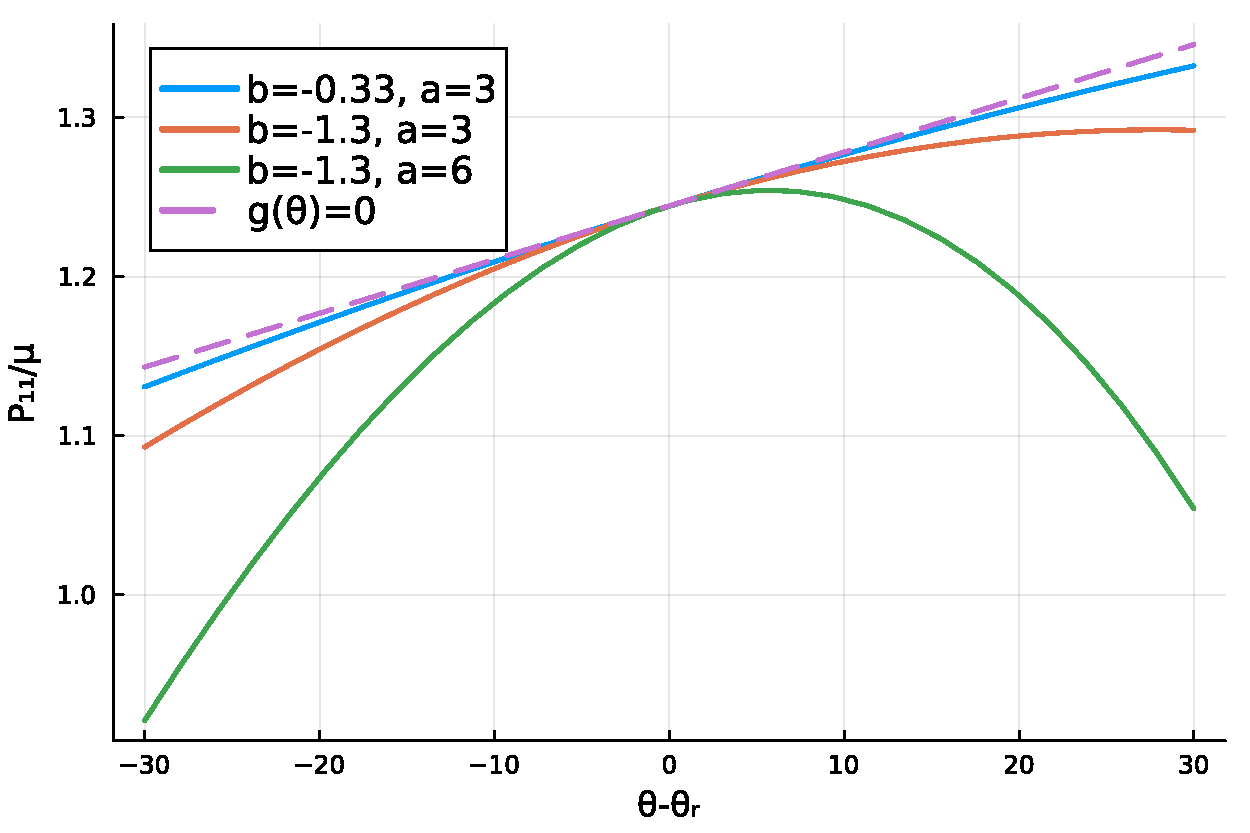
\includegraphics[width=0.45\textwidth]{Figures/NonlinearBehaviourTemperature}&
		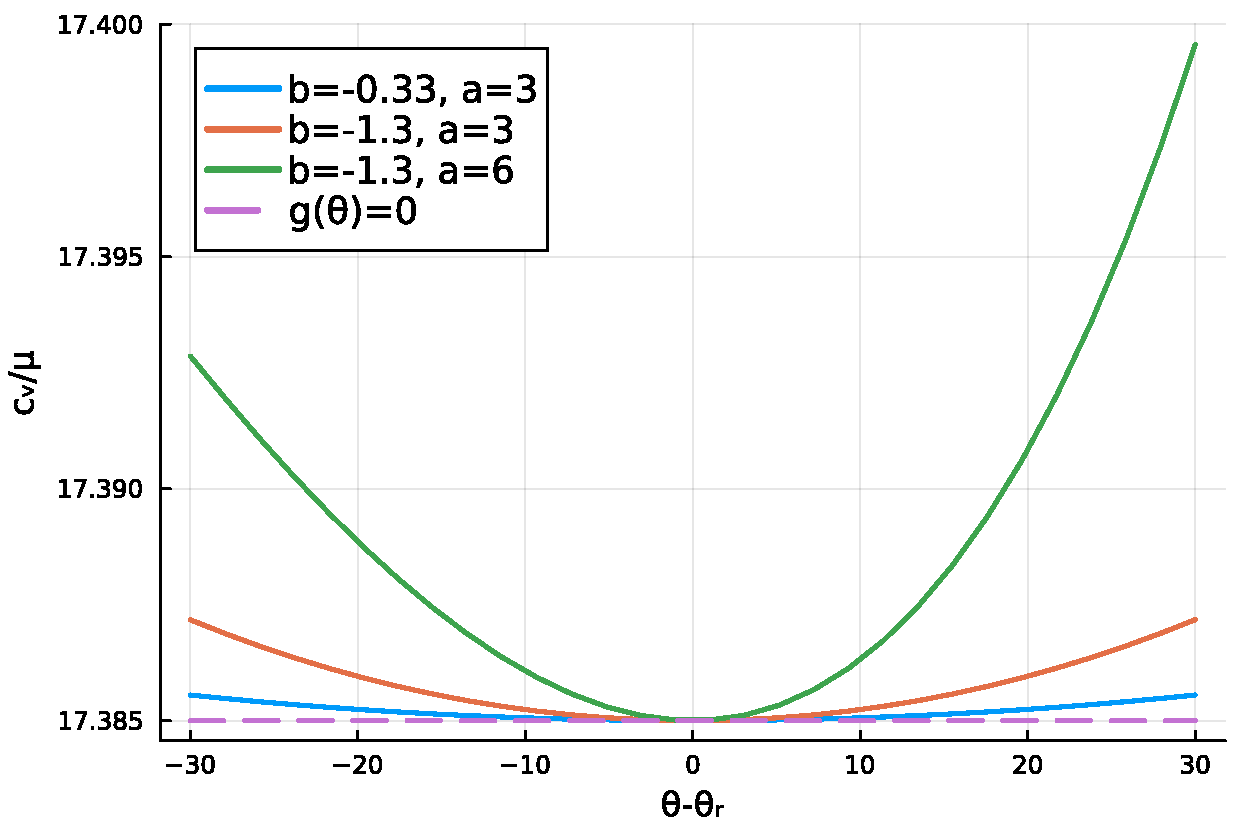
\includegraphics[width=0.45\textwidth]{Figures/Cv_vs_Temperature}\\
		%
		(a)  &  (b)
		%
	\end{tabular}
	\vspace{-2mm}
	\caption{a) Nonlinear behaviour of stress (component $11$ of $\vect{P}$) with respect to temperature; b) Nonlinear behaviour of $c_v$ with respect to $\theta$. In both cases  $\vect{F}$ and $\vect{E}_0$ have been fixed to the values given in \eqref{eqn:fixed values} where the purely mechanical and electro-mechanical isothermal potential,  $\Psi_m$ and $\Psi_{em}$ correspond with a Mooney-Rivlin model and  an ideal dielectric elastomer model, respectively.}
	\label{fig:model}
\end{figure}


\subsection{Specific forms of $\Psi_m(\vect{F})$ and $\Psi_{em}(\vect{F},\vect{E}_0)$}\label{sec:ground truth models}

In the generic expression of the Helmholtz energy density, $\Psi(\vect{F},\vect{E}_0,\theta)$, as presented in equation \eqref{eqn:additive decomposition}, we have systematically defined all terms except for $\Psi_{m}(\vect{F})$ and $\Psi_{em}(\vect{F},\vect{E}_0)$. For these two potentials, we have explored a broad spectrum of models that characterize the constitutive behavior of ideal dielectric elastomers under isothermal conditions. Specifically, for the purely mechanical contribution $\Psi_m(\vect{F})$, we have examined various hyperelastic potentials listed in Table \ref{table:mechanical potentials}, which include: 
 Mooney-Rivlin model; Quadratic Mooney-Rivlin model; Gent model;  Yeoh model; Arruda-Boyce model; Hyperelastic potentials for transverse isotropy. Table \ref{table:mechanical potentials}  presents the values of the material parameters employed in defining each of the aforementioned models. 

\begin{table}[htbp!]
	\centering
%	\arrayrulecolor{black} % Border color
%	\arrayrulewidth=1pt    % Border width
	\begin{tabular}{c c}
\rowcolor{gray!30}	\multicolumn{2}{c}{Mechanical isothermal Helmholtz free energy $\Psi_{m}$}		\\	
\midrule
\rowcolor{gray!30} {Name of the model}   &  Invariant representation		\\	
%
       \midrule % Border width
%
Mooney-Rivlin (MR) & $\mathbb{U}_{\Psi}  = \frac{\mu_1}{2} \left(I_{\Psi_1} - 3 \right) + \frac{\mu_2}{2} \left(I_{\Psi_2} - 3 \right) - \left( \mu_1 + 2\mu_2 \right) \text{ln} \left(I_{\Psi_3} \right) + \frac{\lambda}{2}  \left( I_{\Psi_3} - 1 \right)^2$\\
%
%    	\arrayrulecolor{black} % Border color
%	\begin{center}
\multicolumn{2}{c}{}\\
\multicolumn{2}{c}{\begin{tabular}{@{}lllll@{}}
		\toprule
		Parameter: & $\mu_1$  & $\mu_2$ & $\lambda$ & $\varepsilon$\\
		\midrule
		Value:    & $0.5$   & $0.5$  & $5$  & $1$\\
		\bottomrule
	\end{tabular}}\\

       \midrule % Border width

%
Quadratic MR (QMR)  &  $\mathbb{U}_{\Psi} = \frac{\mu_1}{2} \left(I_{\Psi_1} \right)^2 + \frac{\mu_2}{2} \left(I_{\Psi_2} \right)^2 - 6 \left( \mu_1 + 2\mu_2 \right) \text{ln} \left(I_{\Psi_3} \right) + \frac{\lambda}{2}  \left( I_{\Psi_3} - 1 \right)^2 $\\
%
%
\multicolumn{2}{c}{}\\

\multicolumn{2}{c}{\begin{tabular}{@{}lllll@{}}
		\toprule
		Parameter: & $\mu_1$  & $\mu_2$ & $\lambda$ & $\varepsilon$\\
		\midrule
		Value:    & $0.5$   & $0.5$  & $5$  &  $1$ \\
		\bottomrule
\end{tabular}}\\

%
%
       \midrule % Border width
       %
       %
       %
Gent (G)  &  $\mathbb{U}_{\Psi} = - \frac{\mu }{2}  J_m\text{ln}\left( 1 - \frac{I_{\Psi_1} - 3}{J_m} \right) - \mu \text{ln} \left(I_{\Psi_3} \right) + \frac{\lambda}{2}  \left( I_{\Psi_3} - 1 \right)^2 $\\
%
%
\multicolumn{2}{c}{}\\

\multicolumn{2}{c}{	\begin{tabular}{@{}lllll@{}}
		\toprule
		Parameter: & $\mu$  & $J_m$ & $\lambda$ & $\varepsilon$\\
		\midrule
		Value:    & $1$   & $19$ & $5$ & $1$ \\
		\bottomrule
\end{tabular}}\\
%
\midrule % Border width
Yeoh (Y) &  $\mathbb{U}_{\Psi} = C_{10} \left( I_{\Psi_1} - 3 \right) + C_{20} \left( I_{\Psi_1} - 3 \right)^2 + C_{30} \left( I_{\Psi_1} - 3 \right)^3 $\\&
$- 2 C_{10} \text{ln} \left(I_{\Psi_3} \right) + \frac{\lambda}{2}  \left( I_{\Psi_3} - 1 \right)^2  $\\
%
%
\multicolumn{2}{c}{}\\

\multicolumn{2}{c}{	\begin{tabular}{@{}llllll@{}}
		\toprule
		Parameter: & $C_{10}$  & $C_{20}$ & $C_{30}$ & $\lambda$ & $\varepsilon$\\
		\midrule
		Value:    & $1$   & $1$  & $1$ & $5$ & $1$  \\
		\bottomrule
	\end{tabular}}\\
%
\midrule % Border width
%
%
Arruda-Boyce (AB)  &  $\mathbb{U}_{\Psi} = a_1 \left( \beta \left(I_{\Psi_1} \right) \lambda_c \left(I_{\Psi_1} \right) - a_2 \text{ln} \left( \frac{\sinh \left( \beta \left(I_{\Psi_1} \right) \right)}{\beta \left(I_{\Psi_1} \right)} \right) \right)$\\&$ - A \text{ln} \left(I_{\Psi_3} \right) + \frac{\lambda}{2} \left( I_{\Psi_3} - 1 \right)^2  +B $\\
& $
\lambda_c \left(I_{\Psi_1} \right) = \sqrt{\frac{1}{3}}\sqrt{I_{\Psi_1}}; \qquad \mathcal{L}^{-1} \left( x \right) = \frac{3x - x^3}{1 - x^2}; \qquad \beta \left(I_1 \right) = \mathcal{L}^{-1} \left( \frac{\lambda_c \left(I_{\Psi_1} \right)}{a_2} \right) \nonumber
$\\
%
\multicolumn{2}{c}{}\\

\multicolumn{2}{c}{	\begin{tabular}{@{}lllll@{}}
		\toprule
		Parameter: & $a_1$  & $a_2$ & $\lambda$ & $\varepsilon$\\
		\midrule
		Value:    & $2.1899$   & $\sqrt{6}$ & $4.9159$  &  $1$ \\
		\bottomrule
\end{tabular}}\\
%
\midrule % Border width
 %
 %
Trans. Isotropy (TI)  &$
\mathbb{U}_{\Psi} = \frac{\mu_1}{2} \left(I_{\Psi_1} - 3 \right) + \frac{\mu_2}{2} \left(I_{\Psi_2} - 3 \right) - \left( \mu_1 + 2\mu_2 + \mu_3 \right) \text{ln} \left(I_{\Psi_3} \right)$ \\&
$+ \frac{\lambda}{2}  \left( I_{\Psi_3} - 1 \right)^2	+ \frac{\mu_3}{2 \alpha} \Big(\left(I_{\Psi_6} \right)^{\alpha}-1\Big) + \frac{\mu_3}{2 \beta}\Big( \left(I_{\Psi_7} \right)^{\beta} -1\Big)$	 
\\
%
\multicolumn{2}{c}{}\\

\multicolumn{2}{c}{	\begin{tabular}{@{}lllllllll@{}}
		\toprule
		Parameter: & $\mu_1$  & $\mu_2$ & $\mu_3$ & $\lambda$ & $\alpha$ & $\beta$ & $\varepsilon$ & $\bm{N}$ \\
		\midrule
		Value:    & $0.5$   & $0.5$  & $7.5$ & $5$ & $2$ & $2$ & $1$ & $\frac{1}{\sqrt{3}}\begin{bmatrix}1& 1& 1 \end{bmatrix}^T$ \\
		\bottomrule
\end{tabular}}\\
%
\midrule % Border width
       
       
%\end{center}
	\end{tabular}
%
	\caption{The various models used for the isothermal mechanical contribution $\Psi_{m}(\vect{F})$ in \eqref{eqn:additive decomposition}.}
	\label{table:mechanical potentials}
\end{table}


With regards to the electro-mechanical contribution $\Psi_{em}(\vect{F},\vect{E}_0)$, we have considered: Ideal dielectric elastomer; Model with electric saturation, employed by some authors to account for the saturation effects associated with hard inclusions that exhibit electric saturation. Both models and the material parameters used in their definition can be seen in Table \ref{table: electromechanical models}.


\begin{table}[htbp!]
	\centering
	%	\arrayrulecolor{black} % Border color
	%	\arrayrulewidth=1pt    % Border width
	\begin{tabular}{c c}
		\rowcolor{gray!30}	\multicolumn{2}{c}{Electro-mechanical isothermal Helmholtz free energy $\Psi_{em}$}		\\	
		\midrule
		\rowcolor{gray!30} {Name of the model}   &  Invariant representation		\\	
		%
		\midrule % Border width
		%
		Ideal dielectric (ID) & $\mathbb{U}_{\Psi}  = \frac{\mu_1}{2} \left(I_{\Psi_1} - 3 \right) + \frac{\mu_2}{2} \left(I_{\Psi_2} - 3 \right) - \left( \mu_1 + 2\mu_2 \right) \text{ln} \left(I_{\Psi_3} \right) + \frac{\lambda}{2}  \left( I_{\Psi_3} - 1 \right)^2$\\
		%
		%    	\arrayrulecolor{black} % Border color
		%	\begin{center}
		\multicolumn{2}{c}{}\\
		\multicolumn{2}{c}{\begin{tabular}{@{}lllll@{}}
				\toprule
				Parameter: & $\mu_1$  & $\mu_2$ & $\lambda$ & $\varepsilon$\\
				\midrule
				Value:    & $0.5$   & $0.5$  & $5$  & $1$\\
				\bottomrule
		\end{tabular}}\\
		
		\midrule % Border width
		
		%
		Electric Saturation (ES)  &  $\mathbb{U}_{\Psi} = \frac{\mu_1}{2} \left(I_{\Psi_1} \right)^2 + \frac{\mu_2}{2} \left(I_{\Psi_2} \right)^2 - 6 \left( \mu_1 + 2\mu_2 \right) \text{ln} \left(I_{\Psi_3} \right) + \frac{\lambda}{2}  \left( I_{\Psi_3} - 1 \right)^2 $\\
		%
		%
		\multicolumn{2}{c}{}\\
		
		\multicolumn{2}{c}{\begin{tabular}{@{}lllll@{}}
				\toprule
				Parameter: & $\mu_1$  & $\mu_2$ & $\lambda$ & $\varepsilon$\\
				\midrule
				Value:    & $0.5$   & $0.5$  & $5$  &  $1$ \\
				\bottomrule
		\end{tabular}}\\
		
		%
		%
	
		\midrule % Border width
		
		
		%\end{center}
	\end{tabular}
	%
	\caption{The two models used for the isothermal electro-mechanical contribution $\Psi_{em}(\vect{F},\vect{E}_0)$ in \eqref{eqn:additive decomposition}.}
	\label{table: electromechanical models}
\end{table}





\newpage
%



\section{Physics-augmented neural networks constitutive models}\label{eqn:calibration strategies}

In the preceding section, we introduced the general form of the analytical Helmholtz free energy density, which serves as the foundation for generating in-silico data in this section. The primary goal here is to generate such data with Helmholtz free energy densities that are decomposed as per equation \eqref{eqn:additive decomposition}, depending on ${\vect{F},\vect{E}_0,\theta}$. This approach aims to facilitate the construction of neural network surrogates with the capability to depend on the sets $\{\vect{F},\vect{E}_0,\theta\}$, $\{\vect{F},\vect{D}_0,\eta\}$, $\{\vect{F},\vect{D}_0,\theta\}$, or $\{\vect{F},\vect{E}_0,\eta\}$, as outlined in Section \ref{sec:alternative potentials}. These surrogates are consistently denoted as $\Psi_{nn}$, $e_{nn}$, $\Upsilon_{nn}$, or $\Gamma_{nn}$, respectively, in alignment with the potentials described in Section \ref{sec:alternative potentials}.

Crucially, to ensure compliance with fundamental physical principles, such as material frame indifference and material symmetry, we follow an invariant formulation for these potentials, as detailed in Section \ref{subsec:InvariantFormulation}. All of this  is mathematically encapsulated in equation \eqref{eqn:NN objective}, i.e
%
\begin{equation}\label{eqn:NN objective}
\boxed{\begin{aligned}	
&\begin{aligned}
&\text{Ground truth model}\\
&\text{in equation \eqref{eqn:additive decomposition}}
\end{aligned}&
\begin{aligned}
&\text{Family of data-driven neural network}\\
&\text{thermodynamical potentials}
\end{aligned}\\
\hline\\
%
&\Psi(\vect{F},\vect{E}_0,\theta) &\left\{\begin{aligned}
\Psi_{nn}(\vect{F},\vect{E}_0,\theta,\vect{\mathcal{W}})&=\mathbb{U}_{\Psi\,nn}\left(I_{\Psi_1},\dots,I_{\Psi_{n_{\text{inv}}}},\theta\right)\\
e_{nn}(\vect{F},\vect{D}_0,\eta,\vect{\mathcal{W}})&=\mathbb{U}_{e\,nn}\left(I_{e_1},\dots,I_{e_{n_{\text{inv}}}},\eta\right)\\
\Upsilon_{nn}(\vect{F},\vect{D}_0,\theta,\vect{\mathcal{W}})&=\mathbb{U}_{\Upsilon\,nn}\left(I_{\Upsilon_1},\dots,I_{\Upsilon_{n_{\text{inv}}}},\theta\right)\\
\Gamma_{nn}(\vect{F},\vect{E}_0,\eta,\vect{\mathcal{W}})&=\mathbb{U}_{\Gamma\,nn}\left(I_{\Gamma_1},\dots,I_{\Gamma_{n_{\text{inv}}}},\eta\right)
\end{aligned}\right.\\
%
%
\end{aligned}}
\end{equation}
%

In equation \eqref{eqn:NN objective}, $\vect{\mathcal{W}}$ represents the parameters of the neural network, which encompass
%
\begin{equation}
\vect{\mathcal{W}}=\left\{\vect{W}_1,\dots,\vect{W}_{n_{L+1}},\vect{b}_1,\dots,\vect{b}_{n_{L+1}}\right\},
\end{equation}
%
where $\vect{W}_i$ and $\vect{b}_i$ represent the weights and biases associated with layer $i$. As standard in neural networks, for an architecture with $n_{L+1}$ layers, the inputs $\vect{A}_h$ of layer $h$ is obtained through the following expression
%
\begin{equation}
\vect{A}_h   =  \sigma_h\left(\vect{W}_h\vect{A}_{h-1}+\vect{b}_h\right);\qquad h=\{1,\dots,n_{L+1}\}
\end{equation}
%
where 
%
\begin{equation}
\begin{aligned}
\vect{W}_h  \in \mathbb{R}^{n_{h}\times n_{h-1}};\qquad 	\vect{b}_h  \in \mathbb{R}^{n_{h}}
\end{aligned}
\end{equation}
%
where
%
\begin{equation}
n_0  =  n_{\text{inv}}+1;\qquad n_{L+1}=1
\end{equation}
%
where $n_{\text{inv}}=5$ or $n_{\text{inv}}=8$ for isotropy or transverse isotropy, respectively. Furthermore, the vectors $\vect{A}_h$, for $h=L+1$ represents the predicted neural network model whereas for $h=0$, it represents the input of the model, namely 
%
\begin{equation}
\begin{aligned}
\vect{A}_{L+1}&  =  \Psi_{nn}(\vect{F},\vect{E}_0, \theta,\vect{\mathcal{W}});&\qquad \vect{A}_0&  =  \begin{bmatrix}
I_{\Psi_1}  &  I_{\Psi_2} & \dots & I_{\Psi_n} & \theta
\end{bmatrix}\\
%
\vect{A}_{L+1}&  =  e_{nn}(\vect{F},\vect{D}_0, \eta,\vect{\mathcal{W}});&\qquad \vect{A}_0 & =  \begin{bmatrix}
I_{e_1}  &  I_{e_2} & \dots & I_{e_n} & \eta
\end{bmatrix}\\
%
\vect{A}_{L+1}&  = \Upsilon_{nn}(\vect{F},\vect{D}_0, \theta,\vect{\mathcal{W}});&\qquad\vect{A}_0 & =  \begin{bmatrix}I_{\Upsilon_1}  &  I_{\Upsilon_2} & \dots & I_{\Upsilon_n} & \theta
\end{bmatrix}\\
%
\vect{A}_{L+1}&  = \Gamma_{nn}(\vect{F},\vect{E}_0, \eta,\vect{\mathcal{W}});&\qquad\vect{A}_0 & =  \begin{bmatrix}I_{\Gamma_1}  &  I_{\Gamma_2} & \dots & I_{\Gamma_n} & \eta
\end{bmatrix}
\end{aligned}
\end{equation}

In addition, $\sigma_h$ represents the activation function of laer $h$. In our work we have made use of Softplus activation functions, except for the last layer, where we use the identity function, namely
%
\begin{equation}\label{eqn:activation functions}
\sigma_h(x)=\log\left(1 + e^x\right),\,\,h=\{1,\dots,n_L\};\qquad \sigma_{n_{L+1}}(x)=x
\end{equation}

\subsection{Sobolev-type calibration strategy 1}\label{sec:strategy 1}
 
 We begin by describing the fundamental aspects of this strategy (Section \ref{sec:fundamentals strategy 1}), and later, we describe the in-silico data generation strategy used in order to calibrated the models according to this strategy, carried out in Section \ref{sec:data generation strategy 1}.

\subsubsection{Fundamental aspects of the strategy}\label{sec:fundamentals strategy 1}

In this approach, four distinct types of neural network models, namely $\Psi_{nn}(\vect{F},\vect{E}_0,\theta,\vect{\mathcal{W}})$, $e_{nn}(\vect{F},\vect{D}_0,\eta,\vect{\mathcal{W}})$, 
$\Upsilon_{nn}(\vect{F},\vect{D}_0,\theta,\vect{\mathcal{W}})$ or
$\Gamma_{nn}(\vect{F},\vect{E}_0,\eta,\vect{\mathcal{W}})$, are developed with the specific objective of minimizing the discrepancy between: 
%
\begin{itemize}
	\item  the derivatives  $\{\partial_{\vect{F}}\Psi_{nn},-\partial_{\vect{E}_0}\Psi_{nn},-\partial_{\theta}\Psi_{nn}\}$ and $\{\vect{P},\vect{D}_0,\eta\}:=\{\partial_{\vect{F}}\Psi,-\partial_{\vect{E}_0}\Psi,-\partial_{\theta}\Psi\}$
	%
	\item  the derivatives  $\{\partial_{\vect{F}}e_{nn},\partial_{\vect{D}_0}e_{nn},\partial_{\eta}e_{nn}\}$ and $\{\vect{P},\vect{E}_0,\theta\}:=\{\partial_{\vect{F}}\Psi,{\vect{E}_0},\theta\}$
	%
	\item  the derivatives  $\{\partial_{\vect{F}}\Upsilon_{nn},\partial_{\vect{D}_0}\Upsilon_{nn},-\partial_{\theta}\Upsilon_{nn}\}$ and $\{\vect{P},\vect{E}_0,\eta\}:=\{\partial_{\vect{F}}\Psi,{\vect{E}_0},-\partial_{\eta}\Psi\}$	
	%
	\item  the derivatives  $\{\partial_{\vect{F}}\Gamma_{nn},-\partial_{\vect{E}_0}\Gamma_{nn},\partial_{\eta}\Gamma_{nn}\}$ and $\{\vect{P},\vect{D}_0,\theta\}:=\{\partial_{\vect{F}}\Psi,-\partial_{\vect{E}_0}\Psi,\theta\}$	
\end{itemize}
%
showcasing that, regardless of the neural network surrogate employed, the underlying ground truth model remains a Helmholtz free energy density $\Psi(\vect{F},\vect{E}_0,\theta)$ as formulated in equation \eqref{eqn:additive decomposition}. This is illustrated schematically in Figure \ref{fig:strategy 1}.
To accomplish this objective, we define the corresponding Sobolev-type loss functions, with their specific expressions provided in Table \ref{table: sobolev type 1}.

\begin{table}[htbp!]
	\centering
	\begin{tabular}{c c c}
		\toprule
		\rowcolor{gray!30}	\small{} & $\mathcal{L}(\vect{\mathcal{W}})$ &\\
		\midrule
 $\Psi_{nn}$	&	\begin{minipage}{0.72\textwidth}
			\begin{equation*}
			\begin{aligned}
			& \beta_1\frac{\sum_{i=1}^{n_{\text{d}}} \left\| \partial_{\vect{F}}\Psi^{i} - \partial_{\vect{F}} \Psi_{nn}(\vect{X}^i, \vect{\mathcal{W}}) \right\|^2}{\sum_{i=1}^{n_{\text{d}}} \left\| \partial_{\vect{F}}\Psi^{i} \right\|^2}  + \beta_2\frac{\sum_{i=1}^{n_{\text{d}}} \left\| \partial_{\vect{E}_0}\Psi^{i} - \partial_{\vect{E}_0} \Psi_{nn}(\vect{X}^i, \vect{\mathcal{W}}) \right\|^2}{\sum_{i=1}^{n_{\text{d}}} \left\| \partial_{\vect{E}_0}\Psi^{i} \right\|^2} \\
			& + \beta_3\frac{\sum_{i=1}^{n_{\text{d}}} \Big( \partial_{\theta}\Psi^{i} - \partial_{\theta} \Psi_{nn}(\vect{X}^i, \vect{\mathcal{W}}) \Big)^2}{\sum_{i=1}^{n_{\text{d}}} \left( \partial_{\theta}\Psi^{i} \right)^2}
			\end{aligned}
			\end{equation*}
		\end{minipage}  & $\vect{X}^i=\{\vect{F}^i, \vect{E}_0^i, \theta^i\}$ \\
		%	
		\midrule
		%
 $e_{nn}$	&	\begin{minipage}{0.72\textwidth}
			\begin{equation*}
			\begin{aligned}
			& \beta_1\frac{\sum_{i=1}^{n_{\text{d}}} \left\| \partial_{\vect{F}}\Psi^{i} - \partial_{\vect{F}} e_{nn}(\vect{X}^i, \vect{\mathcal{W}}) \right\|^2}{\sum_{i=1}^{n_{\text{d}}} \left\| \partial_{\vect{F}}\Psi^{i} \right\|^2}  + \beta_2\frac{\sum_{i=1}^{n_{\text{d}}} \left\| \vect{E}_0^{i} - \partial_{\vect{D}_0} e_{nn}(\vect{X}^i, \vect{\mathcal{W}}) \right\|^2}{\sum_{i=1}^{n_{\text{d}}} \left\| \vect{E}_0^{i} \right\|^2} \\
			& + \beta_3\frac{\sum_{i=1}^{n_{\text{d}}} \left( \theta^{i} - \partial_{\eta} e_{nn}(\vect{X}^i, \vect{\mathcal{W}}) \right)^2}{\sum_{i=1}^{n_{\text{d}}} \left( \theta^{i} \right)}
			\end{aligned}
			\end{equation*}
		\end{minipage}  & $\vect{X}^i=\{\vect{F}^i, -\partial_{\vect{E}_0}\Psi^i, -\partial_{\theta}\Psi^i\}$ 	\\
		%
		\midrule
		%
 $\Upsilon_{nn}$ &		\begin{minipage}{0.68\textwidth}
			\begin{equation*}
			\begin{aligned}
			& \frac{\sum_{i=1}^{n_{\text{d}}} \left\| \partial_{\vect{F}}\Psi^{i} - \partial_{\vect{F}} \Upsilon_{nn}(\vect{X}^i, \vect{\mathcal{W}}) \right\|^2}{\sum_{i=1}^{n_{\text{d}}} \left\| \partial_{\vect{F}}\Psi^{i} \right\|^2}  + \frac{\sum_{i=1}^{n_{\text{d}}} \left\| \vect{E}_0^{i} - \partial_{\vect{D}_0} \Upsilon_{nn}(\vect{X}^i, \vect{\mathcal{W}}) \right\|^2}{\sum_{i=1}^{n_{\text{d}}} \left\| \vect{E}_0^{i} \right\|^2} \\
			& + \frac{\sum_{i=1}^{n_{\text{d}}} \left( \partial_{\theta}\Psi^{i} - \partial_{\theta} \Upsilon_{nn}(\vect{X}^i, \vect{\mathcal{W}}) \right)^2}{\sum_{i=1}^{n_{\text{d}}} \left( \partial_{\theta}\Psi^{i} \right)^2}
			\end{aligned}
			\end{equation*}
		\end{minipage}  & $\vect{X}^i=\{\vect{F}^i, -\partial_{\vect{E}_0}\Psi^i, \theta^i\}$ 	\\
		%
		\midrule
		%
 $\Gamma_{nn}$	&	\begin{minipage}{0.68\textwidth}
			\begin{equation*}
			\begin{aligned}
			& \frac{\sum_{i=1}^{n_{\text{d}}} \left\| \partial_{\vect{F}}\Psi^{i} - \partial_{\vect{F}} \Gamma_{nn}(\vect{X}^i, \vect{\mathcal{W}}) \right\|^2}{\sum_{i=1}^{n_{\text{d}}} \left\|\partial_{\vect{F}}\Psi^{i} \right\|^2}  + \frac{\sum_{i=1}^{n_{\text{d}}} \left\| \partial_{\vect{E}_0}\Psi^{i} - \partial_{\vect{E}_0} \Gamma_{nn}(\vect{X}^i, \vect{\mathcal{W}}) \right\|^2}{\sum_{i=1}^{n_{\text{d}}} \left\| \partial_{\vect{E}_0}\Psi^{i} \right\|^2} \\
			& + \frac{\sum_{i=1}^{n_{\text{d}}} \left( \theta^{i} - \partial_{\eta} \Gamma_{nn}(\vect{X}^i, \vect{\mathcal{W}}) \right)^2}{\sum_{i=1}^{n_{\text{d}}} \left( \theta^{i} \right)^2}
			\end{aligned}
			\end{equation*}
		\end{minipage} & $\vect{X}^i=\{\vect{F}^i, \vect{E}_0^i, -\partial_{\theta}\Psi^i\}$	\\
		\midrule
		
		
		%
	\end{tabular}
	\caption{Loss functions $\mathcal{L}(\vect{\mathcal{W}})$ used for the calibration of the various type of neural network-based surrogate potentials, i.e. $\Psi_{nn}$, $e_{nn}$, $\Upsilon_{nn}$ or $\Gamma_{nn}$, for the case of Sobolev-type training strategy 1. All the potentials have been calibrated with data obtained from Helmholtz free energy density ground truth models, i.e. $\Psi$. The index $i$ represents in-silico data number $i$, and $n_d$ the number of data used for calibration.}
	\label{table: sobolev type 1}
\end{table}






\begin{figure}[htpb!]
	\centering
	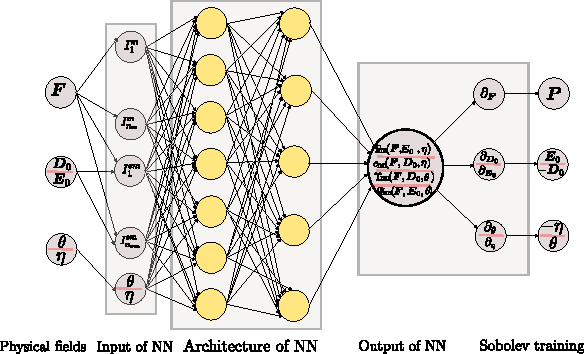
\includegraphics[width=0.85\textwidth]{Figures/InkScape/NN_1}\\
	\vspace{-2mm}
	\caption{Simplified structure of the neural network architecture used for calibration of the four neural network-based surrogate potentials i.e. $\Psi_{nn}$, $e_{nn}$, $\Upsilon_{nn}$ or $\Gamma_{nn}$, for the case of Sobolev-type training strategy 1.}
	\label{fig:strategy 1}
\end{figure}


\subsubsection{Polyconvexity of neural network-based potentials}

Sections \ref{sec:helmholtz} and \ref{sec:alternative potentials} described the desired convexity/convexity conditions that the four possible neural network-based thermodycanimical potentials, namely $\Psi(\vect{F},\vect{E}_0,\theta)$, $e\vect{F},\vect{D}_0,\eta)$, $\Upsilon(\vect{F},\vect{D}_0,\theta)$ or $\Gamma(\vect{F},\vect{E}_0,\theta)$ should satisfy. 
Enforcing simultaneous convexity and convexity across multiple physics, as required for the three potentials $\Psi(\vect{F},\vect{E}_0,\theta)$,  $\Upsilon(\vect{F},\vect{D}_0,\theta)$ or $\Gamma(\vect{F},\vect{E}_0,\theta)$, presents a complex challenge. This difficulty arises whether the model is derived from a phenomenological explicit representation or constructuted using neural network frameworks. However, the direct imposition of convexity exclusively, or more specifically, polyconvexity in the sense of equation \eqref{eqn:polyconvexity}, proves to be more tractable. Building on the work of XX and extending it from electro-mechanics to the thermo-electro-mechanical context, a sufficient condition to ensure polyconvexity of the neural network-based potential $e_{nn}(\vect{F},\vect{D}_0,\eta)$ is the positiveness of the weights $\vect{W}_{h}$ and the monotonically increasing nature of the activation functions, namely
%
\begin{equation}
	\left(\vect{W}_h\right)_{ij}>0;\qquad \sigma^{\prime}_h(x)>0,\forall x;\qquad  h=\left\{1,\dots,n_{L+1}\right\}
\end{equation}

Notice that the first condition can be imposed as a penalty term in the objective function, leading to the augmented objective function $\widetilde{\mathcal{L}}(\vect{\mathcal{W}})$ defined as
%
\begin{equation}
	\widetilde{\mathcal{L}}(\vect{\mathcal{W}})=\mathcal{L}(\vect{\mathcal{W}}) + \frac{\kappa}{2} \sum_{i}\Big(\min\left(\left(\vect{\mathcal{W}}_v\right)_i,0\right)\Big)^2
\end{equation}
%
where $\mathcal{L}(\vect{\mathcal{W}})$ is defined as in Table \ref{table: sobolev type 1}, $\vect{\mathcal{W}}_v$ represents the concatenation of all vectorized weights $\vect{\mathcal{W}}_h$, $h=\{1,\dots,n_{L+1}\}$, and $\kappa$, the penalty parameter. Furthermore, notice that increasing monotonicity is satisfied by the activation functions chosen in equation \eqref{eqn:activation functions}. In this work, we will explore the accuracy of neural network-based $e_{nn}(\vect{F},\vect{D}_0,\eta)$ potentials with and without the additional penalty term enforcing the polyconvexity condition. This will be futher discussed in Section \ref{sec:polyconvexity}.





\subsubsection{In-silico data generation strategy}\label{sec:data generation strategy 1}

In this section, we present the procedure used for generating synthetic data for the training strategy denoted as strategy 1. For that, we have made use of the generic form of the Helmholtz free energy density in equation \eqref{eqn:additive decomposition}, and a variety of models for the isothermal purely mechanical and electro-mechanical contributions $\Psi_m(\vect{F}$ (see Table \ref{table:mechanical potentials}) and $\Psi_{em}(\vect{F},\vect{E}_0)$ (refer to Table \ref{table: electromechanical models}).

To acquire the dataset, we have adhered to the procedure outlined in \cite{OKunc_19_01}, extended to the coupled context of thermo-electro-mechanics. The deformation gradient tensor $\vect{F}$ is parameterized via a  chosen set of deviatoric directions, amplitudes, and Jacobians ($J$, i.e., the determinant of $\vect{F}$). The process of generating sample points for deviatoric directions, amplitudes, and Jacobians is elucidated in Algorithm \ref{alg:sample_generation}. Similarly, the electric displacement $\vect{E}_0$ (for the neural network-based potentials $\Psi_{nn}(\vect{F},\vect{E}_0,\theta)$ and $\Upsilon_{nn}(\vect{F},\vect{E}_0,\eta)$) or $\vect{D}_0$ (for the neural network-based potentials $e_{nn}(\vect{F},\vect{D}_0,\eta)$ and $\Gamma_{nn}(\vect{F},\vect{D}_0,\theta)$) is also parametrised in terms of unitary directions and amplitudes.
Concerning the deviatoric directions for $\vect{F}$, denoted as $\vect{V_F}$ we formulate them using a spherical parametrization in $\mathbb{R}^5$, precisely representing these directions using five pertinent angular measures ($\phi_1, \phi_2, \phi_3, \phi_4, \phi_5\in[0,2\pi]\times[0,\pi]\times[0,\pi]\times[0,\pi]\times[0,\pi]$) within this 5-dimensional space.  For the directions employed for the parametrisation of $\vect{E}_0$  or $\vect{D}_0$ (depending on the dependence on the electrical physics of the neural network-based potential), denoted as $\vect{V}_{\vect{E}_0}$ or $\vect{V}_{\vect{D}_0}$, respectively, these are created using a spherical parametrization in $\mathbb{R}^3$, using as angular measures $(\theta,\psi)\in[0,2\pi]\times[0,\pi]$, namely
%
%

\begin{algorithm}
	\caption{Pseudo-code for sample generation}
	\label{alg:sample_generation}
	
	\begin{algorithmic}[1]
		\State Generate deformation gradient tensors $\vect{F}$ according to:
		
		\begin{algorithmic}[1]
			\State Set the number of amplitudes, directions and determinants: $\{ n_{\bm{t}_{\vect{F}}}, n_{\bm{V}_{\vect{F}}}, n_{\bm{J}_{\vect{F}}}\}$;
			
			\State Initialise a vector of Latin Hypercube Sampled angles: $\bm{\phi}_1 = [0,2\pi]_{n_{\bm{V_F}} \times 1}$ and  $\bm{\phi}_{2,...,4} = [0,\pi]_{n_{\bm{V_F}} \times 1}$;
			
			\State Construct the directions, $\bm{V}_{F}$, using $\bm{\phi}_1, \dots, \bm{\phi}_4$ by means of an extended Spherical parametrisation in $\mathbb{R}^5$ - detailed in (\ref{eqn:spherical_parametersisation});
			
			\State Evaluate the deformation gradient tensors, $\bm{{F}}$ - detailed in Algorithm \ref{alg:F_construction};
		\end{algorithmic}
		
		\State{Generate electric field vectors $\vect{E}_0$ (or $\vect{D}_0$) according to:}
		
		\begin{algorithmic}[1]
			\State Set the amplitudes and directions: $\{n_{\bm{t}_{\vect{E}_0}},  n_{\bm{V}_{\vect{E}_0}}\}$;
			
			\State Initialise a vector of Latin Hypercube Sampled angles: $\bm{\psi}_1 = [0,2\pi]_{n_{\bm{V}_{\vect{E}_0}} \times 1}$ and  $\bm{\psi}_{2} = [0,\pi]_{n_{\bm{V}{\vect{E}_0}} \times 1}$;
			
			\State Construct the directions, $\bm{V}_{\bm{E}_0}$ (or $\vect{V}_{\vect{D}_0}$), using $\bm{\psi}_1, \bm{\psi}_2$ by means of a Spherical parametrisation in $\mathbb{R}^3$;
			
			\State Evaluate the deformation $\bm{{E}}_0$ (or $\bm{{D}}_0$) - detailed in Algorithm \ref{alg:F_construction};
		\end{algorithmic}
		
		\State Generate temperature data $\theta$ (or entropy $\eta$) according to:
		
		\begin{algorithmic}[1]
			\State Set the maximum temperature difference with respect to $\theta_R$, denoted $\Delta\theta$. Then define the minimum and maximum values of $\theta$: $\theta_R-\Delta\theta$ and $\theta_R+\Delta\theta$; For $\eta$-based potentials, set $\eta_{\text{min}}$ and $\eta_{\text{max}}$
			
			\State Set number of temperatures $n_{\theta}$ (or $n_{\eta}$);
			
			\State Generate $n_{\theta}$ uniformly distributed temperature (or randomly) in the interval $(\theta_R-\Delta\theta,\theta_R+\Delta\theta)$; For $\eta$-based potentials, the interval is $(\eta_{\text{min}},\eta_{\text{max}})$
		\end{algorithmic}
		
		\State Generate combination of data of $\{\vect{F},\vect{E}_0,\theta\}$ (or any other combination, for instance $\{\vect{F},\vect{D}_0,\eta\}$)
	\end{algorithmic}
	
\end{algorithm}


%\input{section/05_Numerical_Examples/numerical_examples_sample_gen_algorithm}


%
\begin{equation}
\label{eqn:spherical_parametersisation}
\bm{V}_{\vect{F}}^i = 
\begin{bmatrix}
\cos{\phi_1^i} \\
\sin{\phi_1^i}\cos{\phi_2^i} \\
\sin{\phi_1^i}\sin{\phi_2^i}\cos{\phi_3^i} \\
\sin{\phi_1^i}\sin{\phi_2^i}\sin{\phi_3^i}\cos{\phi_4^i} \\
\sin{\phi_1^i}\sin{\phi_2^i}\sin{\phi_3^i}\sin{\phi_4^i}
\end{bmatrix};\,\, 1\leq i\leq n_{\bm{V_F}};\qquad 
%	
\bm{V}_{\vect{E}_0}^i=\begin{bmatrix}
\cos\psi_1^i\sin\psi_2^i\\  \sin\psi_1^i\sin\psi_2^i\\  \cos\psi_2^i\end{bmatrix};\,\, 1\leq i\leq n_{\bm{V}_{\vect{E}_0}}
\end{equation} 




Once the sample is generated following Algorithm \ref{alg:sample_generation}, the reconstruction of the deformation gradient tensor $\vect{F}$ and of $\vect{D}_0$ becomes possible at each of the sampling points. This reconstruction process is demonstrated in Algorithm \ref{alg:F_construction}, where $\bm{\Uppsi}$ represents the basis for symmetric and traceless tensors (refer to Appendix \ref{sec:appendix_basis_symm_traceless_tensors} for details on $\bm{\Uppsi}$). For the temperature field $\theta$, data generation has been carried out by predefining the maximum difference with respect to the reference temperature $\theta_R$. This approach establishes the lower and upper bounds $\theta_R-\Delta\theta$ and $\theta_R+\Delta\theta$.  Consequently, the data for this field is generated either uniformly distributed within this interval or randomly sampled across the defined range.




\begin{algorithm}[htbp!]
	\caption{Pseudo-code for construction of the set of deformation gradient tensors and electric  fields $\vect{E}_0$ (similarly for $\vect{D}_0$)}
	\label{alg:F_construction}  
	\begin{algorithmic}[1]                                                     
		\For{$i = 1:n_{\bm{V_F}}$}
		
		\For{$j = 1:n_J$}
		
		\For{$k = 1:n_{\bm{t_F}}$}
		
		\State $\bm{F} = J_j^{1/3} \exp\left([\vect{t}_{\vect{F}}]_k \left[\sum_{m = 1}^{5} [\vect{V}^i_{\vect{F}}]_m \bm{\Uppsi}_{m}\right] \right)$;	            		
		\EndFor
		\EndFor
		\EndFor
		
		\For{$i = 1:n_{\bm{V}_{\vect{E}_0}}$}		
		\For{$j = 1:n_{\bm{t}_{\vect{E}_0}}$}
\State $\bm{E}_0 = [\vect{t}_{\vect{E}_0}]_j\vect{V}^i_{\vect{E}_0}$;
\EndFor
\EndFor
		
		
		
	\end{algorithmic}
\end{algorithm}                         



\newpage

\subsection{Sobolev-type calibration strategy 2}\label{sec:strategy 2}

The calibration approach outlined in Section \ref{sec:strategy 1}, referred to as calibration strategy 1, is characterized by its remarkable flexibility—enabling the calibration of four distinct types of thermodynamic potentials—and its robustness, as demonstrated in the numerical examples section. However, this approach is subject to criticism when applied to scenarios involving data generated in real-world conditions, as opposed to an in-silico process. While calibration strategy 1 is well-suited for data generated in-silico, as is the case in this study, its applicability may be severely limited when dealing with laboratory-derived data. The primary challenge arises from the requirement for data across six quantities: $\{\vect{F},\vect{E}_0,\theta,\vect{P},\vect{D}_0,\eta\}$. Of these, entropy $(\eta)$ cannot be directly measured in a laboratory setting, which significantly impairs the feasibility of this calibration strategy in practical, real-world scenarios.


To address this limitation, we have developed an alternative strategy that can be applied to both in-silico and experimentally generated data. The key aspect of this approach lies in substituting the only non-measurable field within $\{\vect{F},\vect{E}_0,\theta,\vect{P},\vect{D}_0,\eta\}$, namely $\eta$, with other thermophysical properties that can be directly measured in a laboratory setting. This modification enhances the versatility of the calibration process, making it applicable to real-world experimental data as well as computationally generated scenarios. A suitable physical property to replace $\eta$ is the specific heat capacity $c_v$ (see equation \eqref{eqn:heat capacity}). 

As discussed in Section \ref{sec:ground truth model},  specifically for the generic Helmholtz free energy density considered in this study, $c_v$ may exhibit a nonlinear dependence on the fields fields $\{\vect{F},\vect{E}_0,\theta\}$, as highlighted in the experimental work of XX. Therefore, we consider incorporating data values for $c_v$ at a set of points $\mathcal{G}_{c_v}=\{\vect{X}^1,\dots,\vect{X}^{n_{c_v}}\}$, which includes the reference configuration $\vect{X}^1=\{\vect{I},\vect{0},\theta_R\}$ as well as other possible scenarios
$\vect{X}^i=\{\vect{F}^i,\vect{E}_0^i,\theta^i\}$, with $n_{c_v}$ the number of data points within the set $\mathcal{G}_{c_v}$. However, the available experimental data for $c_v$,  is typically limited to the reference configuration. To better align with conditions more reflective of the experimental setup, we choose to include only the specific heat capacity $c_v$ data corresponding to the reference configuration, i.e., $\mathcal{G}_{c_v}=\vect{X}^1$. Additionally, while entropy $\eta$ cannot be directly measured, it is known to vanish in the reference configuration (see equation \eqref{eqn:reference conditions}).  Thus, this condition can also be incorporated into the calibration strategy.

Notice that this new approach introduces notable differences in the calibration of the potentials that do depend on $\theta$ (i.e $\Psi_{nn}(\vect{F},\vect{E}_0,\theta)$ and $\Upsilon_{nn}(\vect{F},\vect{D}_0,\theta)$) and those which depend on $\eta$ (i.e $e_{nn}(\vect{F},\vect{D}_0,\eta)$ and $\Gamma_{nn}(\vect{F},\vect{E}_0,\eta)$). The main difference resides in the fact that temperature is data which can be measured and therefore, is available in the calibration (for $\Psi_{nn}(\vect{F},\vect{E}_0,\theta)$ and $\Upsilon_{nn}(\vect{F},\vect{D}_0,\theta)$). However, we assume in this approach that the entropy $\eta$ is not measurable and therefore, not readily available. Consequently, the potentials $e_{nn}(\vect{F}, \vect{D}_0, \eta)$ and $\Gamma_{nn}(\vect{F}, \vect{E}_0, \eta)$ must be calibrated in the absence of any information or data regarding the third argument, $\eta$. This inherent limitation necessitates a distinct treatment for the calibration strategy, differentiating between those potentials that depend on $\theta$ (namely, $\Psi_{nn}(\vect{F}, \vect{E}_0, \theta)$ and $\Upsilon_{nn}(\vect{F}, \vect{D}_0, \theta)$) and those that depend on $\eta$ ($e_{nn}(\vect{F}, \vect{D}_0, \eta)$ and $\Gamma_{nn}(\vect{F}, \vect{E}_0, \eta)$).

\subsubsection{Mathematical formulation of the strategy: potentials depending upon $\theta$}\label{sec:strategy 2 theta}

For the temperature dependent potentials, i.e.  $\Psi_{nn}(\vect{F},\vect{E}_0,\theta,\vect{\mathcal{W}})$ and $\Upsilon_{nn}(\vect{F},\vect{D}_0,\theta,\vect{\mathcal{W}})$, this  alternative and more physically oriented calibration approach,  the specific objective is to minimize the discrepancy between: 
%
\begin{itemize}
	\item    \(
	\Psi_{nn}\left\{
	\begin{aligned}
	&\text{the derivatives } \{\partial_{\vect{F}}\Psi_{nn},-\partial_{\vect{E}_0}\Psi_{nn}\} \text{ and } \{\vect{P},\vect{D}_0\}:=\{\partial_{\vect{F}}\Psi,-\partial_{\vect{E}_0}\Psi\}\\
	&\text{the fields } \{-\theta\partial^2_{\theta\theta}\Psi_{nn},-\left.\partial_{\theta}\Psi_{nn}\right\vert_{\vect{I},\vect{0},\theta_R}\} \text{ and } \{c_v,\left.\eta\right\vert_{\vect{I},\vect{0},\theta_R}\}:=\{-\theta\partial^2_{\theta\theta}\Psi,-\left.\partial_{\theta}\Psi\right\vert_{\vect{I},\vect{0},\theta_R}\}\\
	%
	&\{\vect{F},\vect{E}_0,\theta\} \text{ are data }
	\end{aligned}
	\right.
	\)
	
	
 
	%
	%
	\item  \(
	\Upsilon_{nn}\left\{
	\begin{aligned}
	&\text{the derivatives }  \{\partial_{\vect{F}}\Upsilon_{nn},\partial_{\vect{D}_0}\Upsilon_{nn}\} \text{ and } \{\vect{P},\vect{E}_0\}:=\{\partial_{\vect{F}}\Psi,{\vect{E}_0}\}	\\
	%
	&\text{the fields } \{-\theta\partial^2_{\theta\theta}\Upsilon_{nn},-\left.\partial_{\theta}\Upsilon_{nn}\right\vert_{\vect{I},\vect{0},\theta_R}\} \text{ and } \{c_v,\left.\eta\right\vert_{\vect{I},\vect{0},\theta_R}\}:=\{-\theta\partial^2_{\theta\theta}\Psi,-\left.\partial_{\theta}\Psi\right\vert_{\vect{I},\vect{0},\theta_R}\}\\
%
&\{\vect{F},\vect{D}_0,\theta\} \text{ are data }	
	%
 	\end{aligned}
\right.
\)	
	
	

		
		
			
\end{itemize}
%

This is illustrated schematically in Figure \ref{fig:strategy 2}. Notice that, unlike in the preceeding calibration strategy, the unavailability of $\eta$ prevents in to minimise the difference between $\theta$ and the derivatives of the two potentials with respect to $\theta$, namely $-\partial_{\theta}\Psi_{nn}$ and $-\partial_{\theta}\Upsilon_{nn}$. Instead, we have incorporated $c_v$ and $\left.\partial_{\theta}\Psi_{nn}\right\vert_{\vect{I},\vect{0},\theta_R}$
(or $\left.\partial_{\theta}\Upsilon_{nn}\right\vert_{\vect{I},\vect{0},\theta_R}$) in the minimisation problem. This is reflected in the loss function observed in Table \ref{table: sobolev type 2 theta}.

\begin{table}[htbp!]
	\centering
	\begin{tabular}{c c c}
		\toprule
		\rowcolor{gray!30}	\small{} & $\mathcal{L}(\vect{\mathcal{W}})$ &\\
		\midrule
		$\Psi_{nn}$	&	\begin{minipage}{0.75\textwidth}
			\begin{equation*}
			\begin{aligned}
			& \beta_1\frac{\sum_{i=1}^{n_{\text{d}}} \vert\vert \partial_{\vect{F}}\Psi^{i} - \partial_{\vect{F}} \Psi_{nn}(\vect{X}^i, \vect{\mathcal{W}}) \vert\vert^2}{\sum_{i=1}^{n_{\text{d}}} \vert\vert \partial_{\vect{F}}\Psi^{i} \vert\vert^2}  + \beta_2\frac{\sum_{i=1}^{n_{\text{d}}} \vert\vert \partial_{\vect{E}_0}\Psi^{i} - \partial_{\vect{E}_0} \Psi_{nn}(\vect{X}^i, \vect{\mathcal{W}}) \vert\vert^2}{\sum_{i=1}^{n_{\text{d}}} \vert\vert \partial_{\vect{E}_0}\Psi^{i} \vert\vert} \\
			& + \beta_3\frac{\sum_{i=1}^{n_{c_v}} \Big(\theta^i\partial^2_{\theta\theta}\Psi^i- \theta\partial^2_{\theta\theta}\Psi_{nn}(\vect{X}^i, \vect{\mathcal{W}}) \Big)^2}{\sum_{i=1}^{n_{\text{d}}}   \left(\theta^i\partial^2_{\theta\theta}\Psi^i\right)^2} + \beta_4\Big(\left. \partial_{\theta}\Psi_{nn}(\vect{X}^1,\vect{\mathcal{W}})\right\vert_{\vect{I},\vect{0},\theta_R}\Big)^2
			\end{aligned}
			\end{equation*}
		\end{minipage}  & $\vect{X}^i=\{\vect{F}^i, \vect{E}_0^i, \theta^i\}$ \\
		%	
		%
%
\midrule
		%
		$\Upsilon_{nn}$ &		\begin{minipage}{0.75\textwidth}
			\begin{equation*}
			\begin{aligned}
			& \beta_1\frac{\sum_{i=1}^{n_{\text{d}}} \vert\vert \partial_{\vect{F}}\Psi^{i} - \partial_{\vect{F}} \Upsilon_{nn}(\vect{X}^i, \vect{\mathcal{W}}) \vert\vert^2}{\sum_{i=1}^{n_{\text{d}}} \vert\vert \partial_{\vect{F}}\Psi^{i} \vert\vert^2}  + \beta_2\frac{\sum_{i=1}^{n_{\text{d}}} \vert\vert \vect{E}_0^{i} - \partial_{\vect{D}_0} \Upsilon_{nn}(\vect{X}^i, \vect{\mathcal{W}}) \vert\vert^2}{\sum_{i=1}^{n_{\text{d}}} \vert\vert \vect{E}_0^{i} \vert\vert^2} \\
			&  + \beta_3\frac{\sum_{i=1}^{n_{c_v}} \Big(\theta^i\partial^2_{\theta\theta}\Psi^i- \theta\partial^2_{\theta\theta}\Upsilon_{nn}(\vect{X}^i, \vect{\mathcal{W}}) \Big)^2}{\sum_{i=1}^{n_{\text{d}}}   \left(\theta^i\partial^2_{\theta\theta}\Psi^i\right)^2} + \beta_4\Big(\left. \partial_{\theta}\Upsilon_{nn}(\vect{X}^1,\vect{\mathcal{W}})\right\vert_{\vect{I},\vect{0},\theta_R}\Big)^2
			\end{aligned}
			\end{equation*}
		\end{minipage}  & $\vect{X}^i=\{\vect{F}^i, -\partial_{\vect{E}_0}\Psi^i, \theta^i\}$ 	\\
		%
		%
	\midrule
		
		
		%
	\end{tabular}
	\caption{Loss functions $\mathcal{L}(\vect{\mathcal{W}})$ used for the calibration of $\theta$-based neural network-based surrogate potentials, i.e. $\Psi_{nn}$,  $\Upsilon_{nn}$, for the case of Sobolev-type training strategy 2 described in Section \ref{sec:strategy 2 theta}. All the potentials have been calibrated with data obtained from Helmholtz free energy density ground truth models, i.e. $\Psi$. The index $i$ represents in-silico data number $i$, and $n_d$ the number of data used for calibration, whereas $n_{c_v}$ represents the number of data used for the measurement/evaluation of $c_v$.}
	\label{table: sobolev type 2 theta}
\end{table}




\begin{figure}[htpb!]
	\centering
	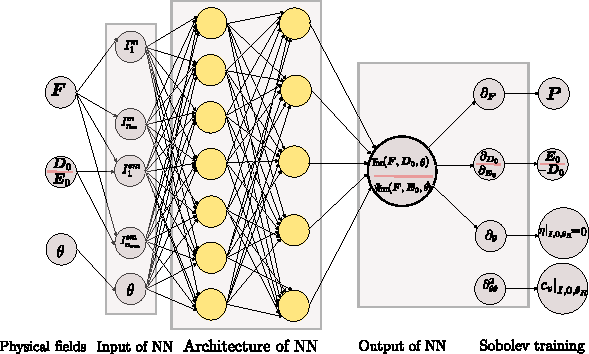
\includegraphics[width=0.85\textwidth]{Figures/InkScape/NN_2}
	\vspace{-2mm}
	\caption{Simplified structure of the neural network architecture used for calibration of the $\theta$-based network-based surrogate potentials i.e. $\Psi_{nn}$, $\Upsilon_{nn}$, for the case of Sobolev-type training strategy 2 in Section \ref{sec:strategy 2 theta}.}
	\label{fig:strategy 2}
\end{figure}




\newpage

\subsubsection{Mathematical formulation of the strategy: potentials depending upon $\eta$}\label{sec:strategy 2 eta}


For the two $\eta$-based potentials, specifically $e(\vect{F}, \vect{D}_0, \eta)$ and $\Gamma(\vect{F}, \vect{E}_0, \eta)$, the second calibration strategy introduces a distinct differentiation compared to the $\theta$-based potentials discussed in Section \ref{sec:strategy 2 theta}. The key distinction lies in the fact that one of the inputs to these potentials, the entropy $\eta$, is not directly available from the given data. Instead, what is provided is the temperature, which corresponds to the derivative of both potentials with respect to $\eta$. Consequently, $\eta$ must be determined implicitly through the nonlinear relationships presented in the third column of the first and third rows of equation \eqref{eqn:piola alternative}. This relationship can be mathematically reformulated as:
%
\begin{equation}\label{eqn:thermo}
\begin{aligned}
&\text{Given } \{\vect{F},\vect{D}_0,\theta\}\, \text{, solve } \eta \text{ from:            }\theta   =  \partial_{\eta}e_{nn}(\vect{F},\vect{D}_0,\eta)\\
%
&\text{Given } \{\vect{F},\vect{E}_0,\theta\}\, \text{, solve } \eta \text{ from:            }\theta   =  \partial_{\eta}\Gamma_{nn}(\vect{F},\vect{E}_0,\eta)
\end{aligned}
\end{equation}




For these entropy-based dependent potentials, i.e.  $e_{nn}(\vect{F},\vect{D}_0,\theta,\vect{\mathcal{W}})$ and $\Gamma_{nn}(\vect{F},\vect{E}_0,\theta,\vect{\mathcal{W}})$, this  alternative and more physically oriented calibration approach,  the specific objective is to satisfy the implicit relationship in \eqref{eqn:thermo} whilst minimizing the discrepancy between: 
%
\begin{itemize}

	
	%
	\item  \(
	e_{nn}\left\{
	\begin{aligned}
	&\text{the derivatives }  \{\partial_{\vect{F}}e_{nn},\partial_{\vect{D}_0}e_{nn},\partial_{\eta}e_{nn}\} \text{ and } \{\vect{P},\vect{E}_0,\theta\}:=\{\partial_{\vect{F}}\Psi,{\vect{E}_0},\theta\}\\
	%
	&\text{the field } \frac{\theta}{\partial^2_{\theta\theta} e} \text{ and } c_v:=-\theta\Psi^2_{\theta\theta}\\
	%
	&\{\vect{F},\vect{D}_0\} \text{ are data }\\
	& \eta \text{ is not data and it is obtained implicitly from } \theta = \partial_{\eta}e_{nn}(\vect{F},\vect{D}_0,\eta)	 
	\end{aligned}
	\right.
	\)
	
	%

	
	\item  \(	\Gamma_{nn}\left\{
	\begin{aligned}
	&\text{the derivatives }   \{\partial_{\vect{F}}\Gamma_{nn},-\partial_{\vect{E}_0}\Gamma_{nn},\partial_{\eta}\Gamma_{nn}\} \text{ and } \{\vect{P},\vect{D}_0,\theta\}:=\{\partial_{\vect{F}}\Psi,-\partial_{\vect{E}_0}\Psi,\theta\}\\
	%
	&\text{the field } \frac{\theta}{\partial^2_{\theta\theta} \Gamma} \text{ and } c_v:=-\theta\Psi^2_{\theta\theta}\\
	%
	&\{\vect{F},\vect{D}_0\} \text{ are data }\\
	& \eta \text{ is not data and it is obtained implicitly from } \theta = \partial_{\eta}\Gamma_{nn}(\vect{F},\vect{E}_0,\eta)	 		
	\end{aligned}
	\right.
	\)	
	
	
	
	
\end{itemize}
%


A second distinguishing feature of the second calibration approach applied to $\eta$-based potentials again arises from the fact that one of the inputs, specifically $\eta$, is not directly available from the data set. In particular, when solving, for example, using a Newton-Raphson numerical scheme to iteratively resolve equation \eqref{eqn:thermo}, certain convexity and stability conditions must be satisfied to ensure the existence of a solution. These conditions are inherently embedded within equation \eqref{eqn:rank one convexity other potentials}, necessitating the convexity of both potentials $e_{nn}$ and $\Gamma_{nn}$ with respect to $\eta$, namely:
%
\begin{equation}\label{eqn:convexity}
\partial^2_{\eta\eta}e_{nn}(\vect{F},\vect{D}_0,\eta)>0;\qquad \partial^2_{\eta\eta} \Gamma_{nn}(\vect{F},\vect{E}_0,\eta)>0
\end{equation}

We found that the numerical solution of \eqref{eqn:thermo} benefits from the imposition of the condition in the reference confuguration in equation \ref{eqn:reference conditions for the different potentials}, namely
%
\begin{equation}\label{eqn:reference eta}
\left.\partial_{\eta}e(\vect{F},\vect{D}_0,\eta)\right\vert_{\vect{I},\vect{0},0}  =  \theta_R;\qquad 
\left.\partial_{\eta}\Gamma(\vect{F},\vect{E}_0,\eta)\right\vert_{\vect{I},\vect{0},0}  =  \theta_R
\end{equation}

To inherently satisfy both conditions \eqref{eqn:reference eta} and \eqref{eqn:convexity} within the neural network-based potentials $e_{nn}$ and $\Gamma_{nn}$, we propose the formulation of modified potentials, denoted as $\widetilde{e}_{nn}$ and $\widetilde{\Gamma}_{nn}$.
%
\begin{equation}\label{eqn:modified potentials}
\begin{aligned}
&\widetilde{e}_{nn}(\vect{F},\vect{D}_0,\eta) =  \underbrace{{e}_{nn}(\vect{F},\vect{D}_0,\eta)}_{\text{Neural network model}} + \underbrace{\left(\theta_R-\left.\partial_{\eta}{e}_{nn}(\vect{F},\vect{D}_0,\eta)\right\vert_{\vect{I},\vect{0},0}\right)\eta}_{\text{Condition enforcement in reference conf.}} + \underbrace{\alpha_{\text{stb}}\frac{\theta_R}{2{c_v}_R}\eta^2}_{\text{Stabilizing term}}\\
%
&\widetilde{\Gamma}_{nn}(\vect{F},\vect{E}_0,\eta) =  \underbrace{{\Gamma}_{nn}(\vect{F},\vect{E}_0,\eta)}_{\text{Neural network model}} + \underbrace{\left(\theta_R-\left.\partial_{\eta}{\Gamma}_{nn}(\vect{F},\vect{D}_0,\eta)\right\vert_{\vect{I},\vect{0},0}\right)\eta}_{\text{Condition enforcement in reference conf.}} + \underbrace{\alpha_{\text{stb}}\frac{\theta_R}{2{c_v}_R}\eta^2}_{\text{Stabilizing term}}
%
\end{aligned}
\end{equation}

In fact, evaluation of the first and second derivative with respect to $\eta$ for both modified potentials in \eqref{eqn:modified potentials} yields

\begin{equation}\label{eqn:conditions imposed}
\begin{aligned}
&\partial_{\eta}\Rightarrow\left\{\begin{aligned}
\partial_{\eta}\widetilde{e}_{nn}(\vect{F},\vect{D}_0,\eta) &=  \partial_{\eta}{e}_{nn}(\vect{F},\vect{D}_0,\eta) + \theta_R-\left.\partial_{\eta}{e}_{nn}(\vect{F},\vect{D}_0,\eta)\right\vert_{\vect{I},\vect{0},0} + \alpha_{\text{stb}}\frac{\theta_R}{{c_v}_R}\eta\\
%
%
\partial_{\eta}\widetilde{\Gamma}_{nn}(\vect{F},\vect{E}_0,\eta) &=  \partial_{\eta}{\Gamma}_{nn}(\vect{F},\vect{E}_0,\eta) + \theta_R-\left.\partial_{\eta}{\Gamma}_{nn}(\vect{F},\vect{E}_0,\eta)\right\vert_{\vect{I},\vect{0},0} + \alpha_{\text{stb}}\frac{\theta_R}{{c_v}_R}\eta\end{aligned}\right.\\
%
%
&\partial^2_{\eta\eta}\Rightarrow\left\{\begin{aligned}
\partial^2_{\eta\eta}\widetilde{e}_{nn}(\vect{F},\vect{D}_0,\eta)& =  \partial^2_{\eta\eta}{e}_{nn}(\vect{F},\vect{D}_0,\eta)+ \underbrace{\alpha_{\text{stb}}\frac{\theta_R}{{c_v}_R}}_{>0}\\
%
\partial^2_{\eta\eta}\widetilde{\Gamma}_{nn}(\vect{F},\vect{E}_0,\eta)& =  \partial^2_{\eta\eta}{\Gamma}_{nn}(\vect{F},\vect{E}_0,\eta)+ \underbrace{\alpha_{\text{stb}}\frac{\theta_R}{{c_v}_R}}_{>0}
%
\end{aligned}\right.
\end{aligned}
\end{equation}


Clearly, evaluation of the first derivative in \eqref{eqn:conditions imposed} in the reference configuration for both potentials leads to the satisfaction of the condition in equation \eqref{eqn:reference eta}, namely
%
\begin{equation}
\begin{aligned}
\left.\partial_{\eta}\widetilde{e}_{nn}(\vect{F},\vect{D}_0,\eta)\right\vert_{\vect{I},\vect{0},0}& =  \left.\partial_{\eta}{e}_{nn}(\vect{F},\vect{D}_0,\eta)\right\vert_{\vect{I},\vect{0},0} + \theta_R-\left.\partial_{\eta}{e}_{nn}(\vect{F},\vect{D}_0,\eta)\right\vert_{\vect{I},\vect{0},0} = \theta_R\\
%
\left.\partial_{\eta}\widetilde{\Gamma}_{nn}(\vect{F},\vect{E}_0,\eta)\right\vert_{\vect{I},\vect{0},0} &=  \left.\partial_{\eta}{\Gamma}_{nn}(\vect{F},\vect{E}_0,\eta)\right\vert_{\vect{I},\vect{0},0} + \theta_R-\left.\partial_{\eta}{\Gamma}_{nn}(\vect{F},\vect{E}_0,\eta)\right\vert_{\vect{I},\vect{0},0} = \theta_R
\end{aligned}
%
\end{equation}


To examine the second derivative in \eqref{eqn:conditions imposed}, it becomes evident that while the second term is positive, there is no guarantee that the overall derivative, specifically $\partial^2_{\eta\eta}\widetilde{e}_{nn}(\vect{F},\vect{D}0,\eta)$ and $\partial^2_{\eta\eta}\widetilde{\Gamma}_{nn}(\vect{F},\vect{E}0,\eta)$, will be positive. The positivity of these derivatives is contingent upon the chosen value of the stabilizing parameter $\alpha{\text{stb}}$. Based on our empirical observations, we have determined that setting $\alpha_{\text{stb}} = 0.25$ suffices to prevent numerical instabilities during the solution of equation \eqref{eqn:thermo}.

The calibration method for the $\eta$-based potentials outlined above is depicted schematically in Figure \ref{fig:strategy 2 eta}. To achieve the primary goal of this calibration approach, we define the associated Sobolev-type loss functions, with their specific formulations detailed in Table \ref{table: sobolev type 2 eta}.







\begin{table}[htbp!]
	\centering
	\begin{tabular}{c c c}
		\toprule
		\rowcolor{gray!30}	\small{} & $\mathcal{L}(\vect{\mathcal{W}})$ &\\
		\midrule
		%
		$e_{nn}$	&	\begin{minipage}{0.65\textwidth}
			\begin{equation*}
			\begin{aligned}
			& \beta_1\frac{\sum_{i=1}^{n_{\text{d}}} \vert\vert \partial_{\vect{F}}\Psi^{i} - \partial_{\vect{F}} e_{nn}(\vect{X}^i, \vect{\mathcal{W}}) \vert\vert^2}{\sum_{i=1}^{n_{\text{d}}} \vert\vert \partial_{\vect{F}}\Psi^{i} \vert\vert^2}  + \beta_2\frac{\sum_{i=1}^{n_{\text{d}}} \vert\vert \vect{E}_0^{i} - \partial_{\vect{D}_0} e_{nn}(\vect{X}^i, \vect{\mathcal{W}}) \vert\vert^2}{\sum_{i=1}^{n_{\text{d}}} \vert\vert \vect{E}_0^{i} \vert\vert^2} \\
			& + \beta_3\frac{\sum_{i=1}^{n_{\text{d}}} \Big( \theta^{i} - \partial_{\eta} e_{nn}(\vect{X}^i, \vect{\mathcal{W}})\Big)^2 }{\sum_{i=1}^{n_{\text{d}}}  \left(\theta^{i}\right)^2 }
			\end{aligned}
			\end{equation*}
		\end{minipage}  & $\vect{X}^i=\{\vect{F}^i, -\partial_{\vect{E}_0}\Psi^i, -\partial_{\theta}\Psi^i\}$ 	\\
		%
		%
		%
		$\Gamma_{nn}$	&	\begin{minipage}{0.68\textwidth}
			\begin{equation*}
			\begin{aligned}
			& \beta_1\frac{\sum_{i=1}^{n_{\text{d}}} \vert\vert \partial_{\vect{F}}\Psi^{i} - \partial_{\vect{F}} \Gamma_{nn}(\vect{X}^i, \vect{\mathcal{W}}) \vert\vert^2}{\sum_{i=1}^{n_{\text{d}}} \vert\vert\partial_{\vect{F}}\Psi^{i} \vert\vert^2}  + \beta_2\frac{\sum_{i=1}^{n_{\text{d}}} \vert\vert \partial_{\vect{E}_0}\Psi^{i} - \partial_{\vect{E}_0} \Gamma_{nn}(\vect{X}^i, \vect{\mathcal{W}}) \vert\vert^2}{\sum_{i=1}^{n_{\text{d}}} \vert\vert \partial_{\vect{E}_0}\Psi^{i} \vert\vert^2} \\
			& + \beta_3\frac{\sum_{i=1}^{n_{\text{d}}} \left( \theta^{i} - \partial_{\eta} \Gamma_{nn}(\vect{X}^i, \vect{\mathcal{W}}) \right)^2}{\sum_{i=1}^{n_{\text{d}}} \left( \theta^{i} \right)^2}
			\end{aligned}
			\end{equation*}
		\end{minipage} & $\vect{X}^i=\{\vect{F}^i, \vect{E}_0^i, -\partial_{\theta}\Psi^i\}$	\\
		\midrule
		
		
		%
	\end{tabular}
	\caption{Loss functions $\mathcal{L}(\vect{\mathcal{W}})$ used for the calibration of $\eta$-based neural network-based surrogate potentials, i.e. $e_{nn}$,  $\Gamma_{nn}$, for the case of Sobolev-type training strategy 2 described in Section \ref{sec:strategy 2 eta}. All the potentials have been calibrated with data obtained from Helmholtz free energy density ground truth models, i.e. $\Psi$. The index $i$ represents in-silico data number $i$, and $n_d$ the number of data used for calibration, whereas $n_{c_v}$ represents the number of data used for the measurement/evaluation of $c_v$.}
	\label{table: sobolev type 2 eta}
\end{table}




\begin{figure}[htpb!]
	\centering
	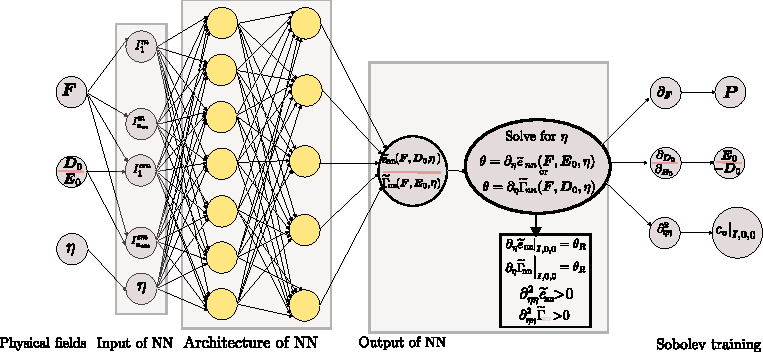
\includegraphics[width=1.0\textwidth]{Figures/InkScape/NN_3}
	\vspace{-2mm}
	\caption{Simplified structure of the neural network architecture used for calibration of the $\eta$-based network-based surrogate potentials i.e. $e_{nn}$, $\Gamma_{nn}$, for the case of Sobolev-type training strategy 2 in Section \ref{sec:strategy 2 eta}. Enforcement of conditions \eqref{eqn:convexity} and \eqref{eqn:reference eta} is carried out through the modifications in equation \eqref{eqn:modified potentials}.}
	\label{fig:strategy 2 eta}
\end{figure}


\subsubsection{In-silico data generation strategy}

In this section, we briefly described the procedure used for generating synthetic data for the calibration strategy denoted as strategy 2. The procedure is entirely the same as for strategy 1, summarised in Algorithm \ref{alg:sample_generation}. The generation of deformation gradient tensors (step 1 in Algorithm \ref{alg:sample_generation}) and electric fields $\vect{E}_0$ or electric displacement fields $\vect{D}_0$ (step 2 in Algorithm \ref{alg:sample_generation}) is entirely the same as for strategy 1 in Algorithm \ref{alg:sample_generation}. The main difference lies with regards step 3 in Algorithm \ref{alg:sample_generation}. We summarise for convenience the steps followed in the data generation procedure for calibration strategy 1, and supplement those for calibration strategy 2, permitting a direct comparison between both strategies:

\vspace{2mm}

\noindent{\textbf{Data generation strategy 1:}}
\vspace{-2mm}
\begin{itemize}
	\item For $\theta$-based potentials, i.e. $\Psi_{nn}(\vect{F},\vect{E}_0,\theta)$ or $\Upsilon_{nn}(\vect{F},\vect{D}_0,\theta)$, fields $\{\vect{F},\vect{E}_0,\theta\}$ or $\{\vect{F},\vect{D}_0,\theta\}$, respectively, are generated as input data according to Algorithm \ref{alg:sample_generation}. Evaluation of the model permits then to synthetically generate the work conjugate fields $\{\vect{P},\vect{D}_0,\eta\}$ or $\{\vect{P},\vect{E}_0,\eta\}$, respectively, as output variables. 
	
	\item For $\eta$-based potentials, i.e. $e(\vect{F},\vect{D}_0,\eta)$ and $\Gamma(\vect{F},\vect{E}_0,\eta)$, the process is the opposite:  $\{\vect{F},\vect{D}_0,\eta\}$ or $\{\vect{F},\vect{E}_0,\eta\}$, respectively, are generated as input data according to Algorithm \ref{alg:sample_generation}. Evaluation of the model permits then to synthetically generate the work conjugate fields $\{\vect{P},\vect{E}_0,\theta\}$ or $\{\vect{P},\vect{D}_0,\theta\}$, respectively, as output variables.	
\end{itemize} 


\vspace{2mm}

\noindent{\textbf{Data generation strategy 2:}}
\vspace{-2mm}

\begin{itemize}
	\item For $\theta$-based potentials, i.e. $\Psi_{nn}(\vect{F},\vect{E}_0,\theta)$ or $\Upsilon_{nn}(\vect{F},\vect{D}_0,\theta)$, data for fields $\{\vect{F},\vect{E}_0,\theta\}$ or $\{\vect{F},\vect{D}_0,\theta\}$, respectively, are generated as input data according to Algorithm \ref{alg:sample_generation}. Then, the fields $\{\vect{P},\vect{D}_0\}$ or $\{\vect{P},\vect{E}_0\}$ (generated as synthetic data through direct evaluation of the analytical model or through experiments), respectively, are considered as output variables. The entropy field $\eta$ is discarded (for synthetic approaches) or directly not available (for experimental procedures). In addition, data for the specific heat capacity $c_v$ is needed (see Section \ref{sec:strategy 2 theta}).
	
	\item For $\eta$-based potentials, i.e. $e(\vect{F},\vect{D}_0,\eta)$ and $\Gamma(\vect{F},\vect{E}_0,\eta)$, data for fields $\{\vect{F},\vect{D}_0,\theta\}$ or $\{\vect{F},\vect{E}_0,\theta\}$, respectively, are generated according to Algorithm \ref{alg:sample_generation}.  Out of the three fields, only two $\{\vect{F},\vect{D}_0\}$ or $\{\vect{F},\vect{D}_0\}$, respectively, are considered to be input variables. The third field, namely $\theta$, is used to solve implicitly the entropy field $\eta$ according to \eqref{eqn:thermo}. Then, the fields  $\{\vect{P},\vect{D}_0\}$ or $\{\vect{P},\vect{E}_0\}$ (generated as synthetic data through direct evaluation of the analytical model or through experiments), respectively, are considered as output variables in conjunction with $\theta$. In addition, data for the specific heat capacity $c_v$ is needed (see Section \ref{sec:strategy 2 theta}).
\end{itemize} 








\section{Finite Element implementation of nonlinear thermo-electro-mechanics}\label{sec:FEM residuals}
%
\subsection{Continuum formulation}
%
%

An objective of this study is to integrate neural network-based potentials, calibrated using the strategies outlined in Section \ref{eqn:calibration strategies}, into a Finite Element computational framework for the numerical modeling of the governing equations presented in \eqref{eqn:local form conservation of linear momentum},
\eqref{eqn:local form Gauss Faraday} and
\eqref{eqn:local form energy}. It is assumed that, irrespective of the chosen thermodynamic potential—whether it be $\Psi(\vect{F},\vect{E}_0,\theta)$, $e(\vect{F},\vect{D}_0,\eta)$, $\Gamma(\vect{F},\vect{E}_0,\eta)$, or $\Upsilon(\vect{F},\vect{D}_0,\theta)$—the corresponding Helmholtz potential, $\Psi(\vect{F},\vect{E}_0,\theta)$, can always be derived via an appropriate Legendre transformation (as shown in equation \eqref{eqn:other potentials}). Based on this, the weak forms of the governing equations \eqref{eqn:local form conservation of linear momentum},
\eqref{eqn:local form Gauss Faraday} and
\eqref{eqn:local form energy} can be formulated as follows:



%In  addition, $H^1$ denotes the Sobolev functional space of square integrable functions and derivatives and $\mathbb{L}_2$, the space of square integrable functions. 
%
\begin{equation}\label{eqn:weak forms for the dynamic formulation}
	\begin{aligned}
%
		\mathcal{W}_{\vect{\phi}} &  = \int_{\mathcal{B}_0}\rho_0\dot{\vect{v}}\cdot\vect{w}_{\vect{\phi}}\,dV + \int_{\mathcal{B}_0}\partial_{\vect{F}}\Psi:\partial_{\vect{X}}\vect{w}_{\vect{\phi}}\,dV\-  -\int_{\mathcal{B}_0}\vect{f}_0\cdot\vect{w}_{\vect{\phi}}\,dV-
		\int_{\partial_{\boldsymbol{t}}\mathcal{B}_0}\vect{t}_0\cdot\vect{w}_{\vect{\phi}}\,dA=0;\\
		%
		\mathcal{W}_{{\varphi}} &  =  -\int_{\mathcal{B}_0}\partial_{\vect{D}_0}\Psi\cdot\partial_{\vect{X}}{w}_{{\varphi}}\,dV +\int_{\mathcal{B}_0}\rho_0^e {w}_{{\varphi}}\,dV+
\int_{\partial_{\omega}\mathcal{B}_0}{\omega}^e_0\cdot{w}_{{\varphi}}\,dA=0;\\		
		%
		\mathcal{W}_{{\theta}}& =  -\int_{\mathcal{B}_0}\theta\dot{\left({\partial_{\theta}\Psi}\right)}w_{\theta}\,dV - \int_{\mathcal{B}_0}\vect{Q}\cdot\vect{\nabla}_0w_{\theta}\,dV - \int_{\mathcal{B}_0}R_{\theta}{w}_{\theta}\,dV - \int_{\partial_{Q}\mathcal{B}_{0}}Q_{\theta}w_{\theta}\,dA=0,
		%
	\end{aligned}
\end{equation}
%
{where
	$\{\vect{\phi},\varphi,\theta\}\in \mathbb{V}^{\vect{\phi}}\times\mathbb{V}^{{\varphi}}\times\mathbb{V}^{\theta}$ and  $\{\vect{w}_{\vect{\phi}},{w}_{{\varphi}},{w}_{\theta}\}\in \mathbb{V}_0^{\vect{\phi}}\times\mathbb{V}_0^{{\varphi}}\times\mathbb{V}_0^{\theta}$\footnote{Notice in that $\vect{\phi}$ must satisfy in addition the condition $J>0$ a.e.}, with}
%
{\begin{equation}\label{eqn:functional spaces}
		\begin{aligned}
			\mathbb{V}^{\vect{\phi}} & = \left\{\vect{\phi}:\mathcal{B}_0\rightarrow \mathbb{R}^3;\,\,\,\,\, \left(\vect{\phi}\right)_{i}\in H^1\left(\mathcal{B}_0\right)\right\};&\quad
			%
%			
			\mathbb{V}_0^{{\vect{\phi}}} & = \left\{\forall\vect{\phi}\in\mathbb{V}^{\vect{\phi}};\,\,\,\,\, \vect{\phi} = \vect{0} \,\,\text{on}\,\,\partial_{\vect{\phi}}\mathcal{B}_0\right\}\\
%						
			\mathbb{V}^{{\varphi}} & = \left\{{\varphi}:\mathcal{B}_0\rightarrow \mathbb{R};\,\,\,\,\, {\varphi}\in H^1\left(\mathcal{B}_0\right)\right\};&\quad			
			%
			\mathbb{V}_0^{{{\varphi}}} & = \left\{\forall{\varphi}\in\mathbb{V}^{\varphi};\,\,\,\,\, {\varphi} = {0} \,\,\text{on}\,\,\partial_{{\varphi}}\mathcal{B}_0\right\}\\
%			
			\mathbb{V}^{{\theta}} & = \left\{\theta:\mathcal{B}_0\rightarrow\mathbb{R};\,\,\,\,\, {\theta}\in H^1\left(\mathcal{B}_0\right)\right\};&\quad
			%
			\mathbb{V}_0^{{\theta}} & = \left\{\forall\theta\in\mathbb{V}^{\theta};\,\,\,\,\,\,\,{\theta} = {0} \,\,\text{on}\,\,\partial_{{\theta}}\mathcal{B}_0\right\}.
			%
		\end{aligned}
\end{equation}}



As standard in finite elements, the domain $\mathcal{B}_0$ described in Section \ref{sec:kinematics} and representing a thermo-elastic continuum is sub-divided into a finite set of non-overlapping elements $e\in \mathbb{E}$ such that 
%
\begin{equation}
\mathcal{B}_0\approx \mathcal{B}_0^h = \bigcup_{e\in\mathbb{E}}   \mathcal{B}^e_{0}.
\end{equation}

The unknown fields $\{\vect{\phi},{\varphi},\theta\}$ in the weak forms $\mathcal{W}_{\vect{\phi}}$, $\mathcal{W}_{{\varphi}}$ and $\mathcal{W}_{{\theta}}$ in \eqref{eqn:weak forms for the dynamic formulation} are discretised employing the following functional spaces $\mathbb{V}^{\vect{\phi}^h}\times\mathbb{V}^{{\varphi}^h}\times\mathbb{V}^{{\theta}^h}$ defined as
%
\begin{equation}\label{eqn:functional spaces for discretisation}
\begin{aligned}
&	\begin{aligned}
\mathbb{V}^{\vect{\phi}^h}& = \{\vect{\phi}\in \mathbb{V}^{\vect{\phi}};\,\,\,\,
\left.\vect{\phi}^h\right\vert_{\mathcal{B}_0^e} = \sum_{a=1}^{n_{\text{node}}^{\vect{\phi}}}N^{\vect{\phi}}_a\vect{\phi}_a\};\qquad
%
%
\mathbb{V}^{{\varphi}^h}& = \{{\varphi}\in \mathbb{V}^{{\varphi}};\,\,\,\,
\left.{\varphi}^h\right\vert_{\mathcal{B}_0^e} = \sum_{a=1}^{n_{\text{node}}^{{\varphi}}}N^{{\varphi}}_a{\varphi}_a\};\\
%
\end{aligned}
\\
%
&\mathbb{V}^{\theta^h} = \{\theta\in \mathbb{V}^{\theta};\,\,\,\,\left.\theta^h\right\vert_{\mathcal{B}_0^e} = \sum_{a=1}^{n_{\text{node}}^{\theta}}N^{\theta}_a\theta_{a}\},
%
%
\end{aligned}
\end{equation}
%
where for any field $\vect{\mathcal{Y}}\in\{\vect{\phi},\varphi,\theta\}$, $n_{\text{node}}^{\vect{\mathcal{Y}}}$ denotes the number of nodes per element of the discretisation associated with the field $\vect{\mathcal{Y}}$ and $N^{\vect{\mathcal{Y}}}_{a}:\mathcal{B}_0^e\rightarrow \mathbb{R}$,  the $a^{th}$ shape function used for the interpolation of  $\vect{\mathcal{Y}}$. 
In addition, $\vect{\mathcal{Y}}_a$ represents the value of the field $\vect{\mathcal{Y}}$ at the $a^{th}$ node of a given finite element. 
Similarly, following a Bubnov-Galerkin approach, the functional spaces for the test functions $\{\vect{w}_{\vect{\phi}},w_{\varphi},w_{\theta}\}\in \mathbb{V}^{\vect{\phi}^h}_0\times \mathbb{V}^{{\varphi}^h}_0\times\mathbb{V}_0^{\theta^h}$ are defined as
%
{\begin{equation}\label{eqn:functional spaces for discretisation virtual}
\begin{aligned}
&	\begin{aligned}
\mathbb{V}_0^{{\vect{\phi}}^h}  = \left\{\forall \vect{\phi}\in\mathbb{V}^{\vect{\phi}^h};\,\,\,\,\, \vect{\phi} = \vect{0} \,\,\text{on}\,\,\partial_{\vect{\phi}}\mathcal{B}_0\right\};\qquad
%
\mathbb{V}_0^{{{\varphi}}^h}  = \left\{\forall {\varphi}\in\mathbb{V}^{{\varphi}^h};\,\,\,\,\, {\varphi} = 0 \,\,\text{on}\,\,\partial_{{\varphi}}\mathcal{B}_0\right\};
	\end{aligned}\\
%
&\mathbb{V}_0^{{\theta}^h}  = \left\{\forall\theta\in\mathbb{V}^{\theta^h};\,\,\,\,\,\,\,{\theta} = {0} \,\,\text{on}\,\,\partial_{{\theta}}\mathcal{B}_0\right\}.
%
\end{aligned}
\end{equation}}

We have made use of a mid point time integrator where the time derivatives $\dot{\vect{v}}$ and $\dot{\eta}$ are replaced by the discrete counterparts according to
%
\begin{equation}\label{eqn:strong form first equations}
\dot{\vect{v}}=\frac{\Delta\vect{v}}{\Delta t};\qquad 
%
\dot{\eta}=\frac{\Delta \eta}{\Delta t},
%
\end{equation}
%
where 
%
\begin{equation}
	\Delta\vect{v} =  \vect{v} - \vect{v}_n;\qquad 
	\Delta\eta =  \eta - \eta_n	
\end{equation}
%
where $\bullet_n$ stands for the value of a field $\bullet$ in the previous time step, and with $\Delta t$ the time step size used for the discretization. Furthermore, the velocity field is related with the deformed mapping $\vect{\phi}$ through the following relationship
%
\begin{equation}
\frac{\Delta\vect{\phi}}{\Delta t} = \vect{v}_{n+1/2}.
\end{equation}
%
where, for any field $\bullet$,  $\bullet_{n+1/2}$ stands for 
%
\begin{equation}
	\bullet_{n+1/2}=\bullet + \bullet_n
\end{equation}

Consideration of the functional spaces for $\{\vect{\phi},{\varphi},\theta\}$ and $\{\vect{w}_{\vect{\phi}},{w}_{{\varphi}},w_{\theta}\}$ in \eqref{eqn:functional spaces for discretisation} and \eqref{eqn:functional spaces for discretisation virtual} enables to obtain the semi-discrete version of $\{\mathcal{W}_{\vect{\phi}},\mathcal{W}_{{\varphi}},\mathcal{W}_{{\theta}}\}$ in \eqref{eqn:weak forms for the dynamic formulation} in terms of their associated elemental residual contributions, namely
%
\begin{equation}
\mathcal{W}_{\vect{\phi}} = \sum_{e=1}^N{\vect{w}_{\vect{\phi}}}_a\cdot\vect{R}_{a,e}^{\vect{\phi}};\qquad
%
\mathcal{W}_{{\varphi}} = \sum_{e=1}^N{{w}_{{\varphi}}}_a\cdot\vect{R}_{a,e}^{{\varphi}};\qquad
%
\mathcal{W}_{\theta} = \sum_{e=1}^N{w_{\theta}}_a{R}_{a,e}^{\theta},
\end{equation}
%
where $N$ denotes the number of elements for the underlying discretisation. 
The residual contributions $\vect{R}^{\vect{\phi}}_{a,e}$ and ${R}^{{\theta}}_{a,e}$ can be expressed as\footnote{For simplicity, the external contributions on the boundary of the continuum and associated with $\vect{t}_0$ and $Q_{\theta}$ have not been included in \eqref{eqn:the residuals}.}
%
\begin{equation}\label{eqn:the residuals}
\begin{aligned}
\vect{R}_{a,e}^{\vect{\phi}} & = \int_{\mathcal{B}^e_0}\rho_0N^a_{\vect{\phi}}\left(2\frac{\Delta\vect{\phi}}{\Delta t^2} - 2\frac{\vect{v}_n}{\Delta t}\right)\,dV + \int_{\mathcal{B}_0^e}\left(\partial_{\vect{F}}\Psi\right)_{n+1/2}\vect{\nabla}_0N^{\vect{\phi}}_a\,dV - \int_{\mathcal{B}_0^e}N^{\vect{\phi}}_{a}\vect{f}_{0_{n+1/2}}\,dV;\\
%
\vect{R}_{a,e}^{{\varphi}} & = -\int_{\mathcal{B}_0^e}\left(\partial_{\vect{E}_0}\Psi\right)_{n+1/2}\vect{\nabla}_0N^{{\varphi}}_a\,dV + \int_{\mathcal{B}_0^e}N^{{\varphi}}_{a}{\rho}^e_{0_{n+1/2}}\,dV;\\
%
R_{a,e}^{\theta} & =-\int_{\mathcal{B}_0}\frac{\theta_{n+1/2}\Delta\left(\partial_{\theta}\Psi\right)}{\Delta t}N^{\theta}_a\,dV - \int_{\mathcal{B}_0}\vect{Q}_{n+1/2}\cdot\vect{\nabla}_0N^{\theta}_a\,dV - \int_{\mathcal{B}_0}{R_{\theta}}_{n+1/2}N^{\theta}_a\,dV.
%
\end{aligned}
\end{equation}
%
where use of equation \eqref{eqn:strong form first equations} has been made of in the inertial term of the residual $\vect{R}^{\vect{\phi}}_{a,e}$ in \eqref{eqn:the residuals}$_a$. 
A consistent linearisation of the nonlinear residual contributions \eqref{eqn:the residuals} has been used in this work. Some details of this linearization can be found in the subsequent section

\subsubsection{Relationship between first and second derivatives of $\Psi(\vect{F},\vect{E}_0,\theta)$ and alternative potentials}

The coupled weak forms presented in equation \eqref{eqn:weak forms for the dynamic formulation} and their residuals in \eqref{eqn:the residuals} are expressed in terms of the derivatives of the Helmholtz potential, $\Psi(\vect{F},\vect{E}_0,\theta)$. However, the fundamental thermodynamic potential governing the constitutive model can alternatively be one of the three other thermodynamic potentials: $e(\vect{F},\vect{D}_0,\eta)$, $\Gamma(\vect{F},\vect{E}_0,\eta)$, or $\Upsilon(\vect{F},\vect{D}_0,\theta)$. In such cases, the derivatives in \eqref{eqn:weak forms for the dynamic formulation} and  \eqref{eqn:the residuals}, specifically $\{\partial_{\vect{F}}\Psi,\partial_{\vect{E}_0}\Psi,\partial_{\theta}\Psi\}$, must be redefined in terms of these alternative potentials. This is accomplished through the appropriate Legendre transformation (refer to \eqref{eqn:other potentials}).



This transformation is not only essential for obtaining the first derivatives but is also crucial for deriving the second derivatives of $\Psi(\vect{F},\vect{E}_0,\theta)$,, i.e., the components of its Hessian, when the primary thermodynamic potential is either $e(\vect{F},\vect{D}_0,\eta)$, $\Gamma(\vect{F},\vect{E}_0,\eta)$, or $\Upsilon(\vect{F},\vect{D}_0,\theta)$. The following sections will detail the procedures for relating both the first derivatives of $\Psi(\vect{F},\vect{E}_0,\theta)$ and the components of its Hessian to their respective counterparts in the potentials $e(\vect{F},\vect{D}_0,\eta)$, $\Gamma(\vect{F},\vect{E}_0,\eta)$, or $\Upsilon(\vect{F},\vect{D}_0,\theta)$.







\subsubsection{Potential $\Upsilon$}

In this case we consider the case when the underlying thermo-electro-mechanical constitutive model is $\Upsilon(\vect{F},\vect{D}_0,\theta)$.  The Legendre transformation in equation \eqref{eqn:other potentials}$_b$ implies that the field
 $\vect{D}_0:=-\partial_{\vect{E_0}}\Psi$ must be considered as a function of the fields $\{\vect{F},\vect{E}_0,\theta\}$, namely
%
\begin{equation}\label{eqn:change of variable for Upsilon}
	\Upsilon=\Upsilon\left(\vect{F},\vect{D}_0(\vect{F},\vect{E}_0,\theta),\theta\right)
\end{equation}
%
and then, $\vect{D}_0:=-\partial_{\vect{E_0}}\Psi$ is implicitly solved from this equation
%
\begin{equation}
	\vect{E}_0=\partial_{\vect{D}_0}\Upsilon\left(\vect{F},\vect{D}_0(\vect{F},\vect{E}_0,\theta),\theta\right)
\end{equation}

Once $\vect{D}_0:=-\partial_{\vect{E_0}}\Psi$ is obtained, $\vect{P}:=\partial_{\vect{F}}\Psi$ and $\eta:=-\partial_{\theta}\Psi$ can be obtained as
%
\begin{equation}
	\begin{aligned}
	\partial_{\vect{F}}\Psi\left(\vect{F},\vect{E}_0,\theta\right)&=\partial_{\vect{F}}\Upsilon\left(\vect{F},\vect{D}_0(\vect{F},\vect{E}_0,\theta),\theta\right);\\
	%
	\partial_{\theta}\Psi\left(\vect{F},\vect{E}_0,\theta\right)&=\partial_{\theta}\Upsilon\left(\vect{F},\vect{D}_0(\vect{F},\vect{E}_0,\theta),\theta\right);
	\end{aligned}
	%
\end{equation}

The components of the Hessian operator of $\Psi(\vect{F},\vect{E}_0,\theta)$, needed for the consistent linearization of \eqref{eqn:the residuals} can then be related to the components of the Hessian operator of $\Upsilon$ by considering $\vect{D}_0$ as a function of $\{\vect{F},\vect{E}_0,\theta\}$, as in \eqref{eqn:change of variable for Upsilon}, yielding the following relationships
%
\begin{equation}
	\begin{aligned}
\partial^2_{\vect{F}\vect{F}}\Psi & =  \partial^2_{\vect{F}\vect{F}}\Upsilon - 
\partial^2_{\vect{F}\vect{D}_0}\Upsilon \cdot \partial_{\vect{E}_0\vect{F}}\Psi;&\quad
%
\partial^2_{\vect{F}\vect{E}_0}\Psi & = 
-\partial^2_{\vect{F}\vect{D}_0}\Upsilon \cdot \partial_{\vect{E}_0\vect{E}_0}\Psi;&\quad
%
\partial^2_{\vect{F}\theta}\Psi & = 
\partial^2_{\vect{F}\theta}\Upsilon
-\partial^2_{\vect{F}\vect{D}_0}\Upsilon\cdot\partial_{\vect{E}_0\theta}\Psi\\
%
%
\partial^2_{\vect{E}_0\vect{F}}\Psi & =  \Big(\partial^2_{\vect{E}_0\vect{F}}\Psi\Big)^T;&\quad
%
\partial^2_{\vect{E}_0\vect{E}_0}\Psi & = -
\Big(\partial^2_{\vect{D}_0\vect{D}_0}\Upsilon\Big)^{-1};&\quad
%
\partial^2_{\vect{E}_0\theta}\Psi & = 
\Big(\partial^2_{\theta\vect{E}_0}\Psi\Big)^T\\
%
%
%
\partial^2_{\theta\vect{F}}\Psi & =\Big(\partial^2_{\theta\vect{F}}\Psi\Big)^T;&\quad
%
\partial^2_{\theta\vect{E}_0}\Psi & = -\partial^2_{\theta\vect{D}_0}\Upsilon\cdot\partial_{\vect{E}_0\vect{E}_0}\Psi ;&\quad
%
\partial^2_{\theta\theta}\Psi & =\partial^2_{\theta\theta}\Upsilon- \partial^2_{\theta\vect{D}_0}\Upsilon\cdot\partial_{\vect{E}_0\theta}\Psi 
%
	\end{aligned}
\end{equation}


\subsubsection{Potential $\Gamma$}

Let us know consider the case when the underlying thermo-electro-mechanical constitutive model is $\Gamma(\vect{F},\vect{E}_0,\eta)$. In this case, the Legendre transformation in equation \eqref{eqn:other potentials}$_c$ implies that the field
$\eta:=-\partial_{\theta}\Psi$ must be considered as a function of the fields $\{\vect{F},\vect{E}_0,\theta\}$, namely
%
\begin{equation}\label{eqn:change of variable for Gamma}
	\Gamma=\Gamma\left(\vect{F},\vect{E}_0,\eta(\vect{F},\vect{E}_0,\theta)\right)
\end{equation}
%
and then, $\eta:=-\partial_{\theta}\Psi$ is implicitly solved from this equation
%
\begin{equation}
	\theta=\partial_{\theta}\Gamma\left(\vect{F},\vect{E}_0,\eta(\vect{F},\vect{E}_0,\theta)\right)
\end{equation}

Once $\eta:=-\partial_{\theta}\Psi$ is obtained, $\vect{P}=\partial_{\vect{F}}\Psi$ and $\vect{D}_0=-\partial_{\vect{E}_0}\Psi$ can be obtained as
%
\begin{equation}
	\begin{aligned}
		\partial_{\vect{F}}\Psi\left(\vect{F},\vect{E}_0,\theta\right)&=\partial_{\vect{F}}\Gamma\left(\vect{F},\vect{D}_0,\eta(\vect{F},\vect{E}_0,\theta)\right);\\
		%
		\partial_{\vect{E}_0}\Psi\left(\vect{F},\vect{E}_0,\theta\right)&=\partial_{\vect{E}_0}\Gamma\left(\vect{F},\vect{D}_0,\eta(\vect{F},\vect{E}_0,\theta)\right);
	\end{aligned}
	%
\end{equation}

The components of the Hessian operator of $\Psi(\vect{F},\vect{E}_0,\theta)$, needed for the consistent linearization of \eqref{eqn:the residuals} can then be related to the components of the Hessian operator of $\Gamma$ by considering $\eta$ as a function of $\{\vect{F},\vect{E}_0,\theta\}$, as in \eqref{eqn:change of variable for Gamma}, yielding the following relationships
%
\begin{equation}
	\begin{aligned}
		\partial^2_{\vect{F}\vect{F}}\Psi & =  \partial^2_{\vect{F}\vect{F}}\Gamma - 
		\partial^2_{\vect{F}\eta}\Gamma \cdot \partial_{\theta\vect{F}}\Psi;&\quad
		%
		\partial^2_{\vect{F}\vect{E}_0}\Psi & = 
\partial^2_{\vect{F}\vect{E}_0}\Gamma		-\partial^2_{\vect{F}\eta}\Gamma \cdot \partial_{\theta\vect{E}_0}\Psi;&\quad
		%
		\partial^2_{\vect{F}\theta}\Psi & = 
		-\partial^2_{\vect{F}\eta}\Gamma\cdot\partial_{\theta\theta}\Psi\\
		%
		%
		\partial^2_{\vect{E}_0\vect{F}}\Psi & =  \Big(\partial^2_{\vect{E}_0\vect{F}}\Psi\Big)^T;&\quad
		%
		\partial^2_{\vect{E}_0\vect{E}_0}\Psi & = -
		\partial^2_{\vect{E}_0\vect{E}_0}\Gamma - 
		\partial^2_{\vect{E}_0\eta}\Gamma \cdot \partial_{\theta\vect{E}_0}\Psi;&\quad
		%
		\partial^2_{\vect{E}_0\theta}\Psi & = 
		-\partial^2_{\vect{E}_0\eta}\Gamma\cdot \partial_{\theta\theta}\Psi \\
		%
		%
		%
		\partial^2_{\theta\vect{F}}\Psi & =\Big(\partial^2_{\theta\vect{F}}\Psi\Big)^T;&\quad
		%
		\partial^2_{\theta\vect{E}_0}\Psi & = \Big(		\partial^2_{\vect{E}_0\theta}\Psi\Big)^T ;&\quad
		%
		\partial^2_{\theta\theta}\Psi & =-\left(\partial^2_{\eta\eta}\Gamma\right)^{-1}
		%
	\end{aligned}
\end{equation}
	

\subsubsection{Potential $e$}

Finally, let us consider the case when the underlying thermo-electro-mechanical constitutive model is $e(\vect{F},\vect{D}_0,\eta)$.
In this case, the Legendre transformation in equation \eqref{eqn:other potentials}$_a$ implies that both fields
$\vect{D}_0:=-\partial_{\vect{E}_0}\Psi$ and $\eta:=-\partial_{\theta}\Psi$ must be considered as functions of the fields $\{\vect{F},\vect{E}_0,\theta\}$, namely
%
\begin{equation}\label{eqn:change of variable for e}
	e=e\left(\vect{F},\vect{D}_0(\vect{F},\vect{E}_0,\theta),\eta(\vect{F},\vect{E}_0,\theta)\right)
\end{equation}
%
and then, $\vect{D}_0:=-\partial_{\vect{E}_0}\Psi$ and $\eta:=-\partial_{\theta}\Psi$ are simultaneously implicitly solved from these equations
%
\begin{equation}
	\begin{aligned}
	\vect{E}_0&=\partial_{\vect{D}_0}e\left(\vect{F},\vect{D}_0(\vect{F},\vect{E}_0,\theta),\eta(\vect{F},\vect{E}_0,\theta)\right);\\
	%
	%
			\theta&=\partial_{\eta}e\left(\vect{F},\vect{D}_0(\vect{F},\vect{E}_0,\theta),\eta(\vect{F},\vect{E}_0,\theta)\right)
	\end{aligned}
\end{equation}

Once $\vect{D}_0:=-\partial_{\vect{E}_0}\Psi$ and $\eta:=-\partial_{\theta}\Psi$ are obtained, $\vect{P}=\partial_{\vect{F}}\Psi$ can be obtained as
%
\begin{equation}
	\begin{aligned}
		\partial_{\vect{F}}\Psi\left(\vect{F},\vect{E}_0,\theta\right)&=\partial_{\vect{F}}e\left(\vect{F},\vect{D}_0(\vect{F},\vect{E}_0,\theta),\eta(\vect{F},\vect{E}_0,\theta)\right).
	\end{aligned}
	%
\end{equation}

The components of the Hessian operator of $\Psi(\vect{F},\vect{E}_0,\theta)$, needed for the consistent linearization of \eqref{eqn:the residuals} can then be related to the components of the Hessian operator of $e$ by considering $\vect{D}_0$ and $\eta$ as functions of $\{\vect{F},\vect{E}_0,\theta\}$, as in \eqref{eqn:change of variable for e}, yielding the following relationships
%
\begin{equation}
	\begin{aligned}
		\partial^2_{\vect{F}\vect{F}}\Psi & =  \partial^2_{\vect{F}\vect{F}}e -
		\partial^2_{\vect{F}\vect{D}_0}e \cdot \partial_{\vect{E}_0\vect{F}}\Psi 
		-
		\partial^2_{\vect{F}\eta}e \cdot \partial_{\theta\vect{F}}\Psi;&\quad
		%
		\partial^2_{\vect{F}\vect{E}_0}\Psi & = 
			-\partial^2_{\vect{F}\vect{D}_0}e \cdot \partial_{\vect{E}_0\vect{E}_0}\Psi-\partial^2_{\vect{F}\eta}e \cdot \partial_{\theta\vect{E}_0}\Psi;\\
		%
				\partial^2_{\vect{F}\theta}\Psi & = 
		-\partial^2_{\vect{F}\vect{D}_0}e \cdot \partial_{\vect{E}_0\theta}\Psi-\partial^2_{\vect{F}\eta}e \cdot \partial_{\theta\theta}\Psi;&\quad
		%
		%
		%
		\partial^2_{\vect{E}_0\vect{F}}\Psi & =  \Big(\partial^2_{\vect{F}\vect{E}_0}\Psi\Big)^T;\\
		%
		\partial^2_{\theta\vect{F}}\Psi & = \Big(
		\partial^2_{\vect{F}\theta}\Psi\Big)^T; &\quad
		%
		%
		%
		&\begin{bmatrix}
			\partial^2_{\vect{E}_0\vect{E}_0}\Psi  &  \partial^2_{\vect{E}_0\theta}\Psi\\
			%
			\partial^2_{\theta\vect{E}_0}\Psi  &  \partial^2_{\theta\theta}\Psi			
		\end{bmatrix}=-\begin{bmatrix}
		\partial^2_{\vect{D}_0\vect{D}_0}e  &  \partial^2_{\vect{D}_0\eta}e\\
		%
		\partial^2_{\eta\vect{D}_0}e  &  \partial^2_{\eta\eta}e			
		\end{bmatrix}^{-1}
		%
	\end{aligned}
\end{equation}
	






%\section{Calibration and validation of the thermodynamic potentials}


This section presents the calibration results for various types of neural network-based thermodynamic potentials, namely $\Psi_{nn}$, $e_{nn}$, $\Gamma_{nn}$ and $\Upsilon_{nn}$, calibrated according to both calibration strategies described in Sections \ref{sec:strategy 1} and \ref{sec:strategy 2}.

\subsection{Calibration strategy 1}

 We begin showing the calibration results by using Sobolev-type calibration strategy 1. 

\subsubsection{Neural network architecture's influence: $\Psi_{nn}$ neural network-based ground truth models}

The objective of this preliminary study is to investigate a specific neural network-based thermodynamic potential, namely $\Psi_{nn}(\vect{F},\vect{E}_0,\theta)$. Our focus is to assess how variations in the neural network architecture influence the accuracy of the potential's calibration. The network architecture is characterized by the number of layers, $n_L+1$, and an equal number of neurons per layer, denoted as $n_n$. By varying these parameters, we track the $R^2$ values of the second-order derivatives of the potential--$R^2$ in the derivatives of the potential, namely $R^2(\partial^2_{\vect{F}}\Psi_{nn})$, $R^2(\partial^2_{\vect{E}_0}\Psi_{nn})$ and $R^2(\partial^2_{\theta}\Psi_{nn})$--for both training and testing datasets. It is important to note that the training data, used for calibrating the potential across all architectures, constitutes  $20\%$ of the testing dataset.

Table \ref{table: results calibration strategy 1} shows the results obtained for the calibrated models $\Psi_{nn}$, not only across different neural network architectures but also when employing the various models described in Section  \ref{sec:ground truth models}. These models represent both the purely mechanical and electro-mechanical contributions of the ground truth Helmholtz strain energy model used for the calibration of all the potentials. The results obtained in this table indicate that in general, the optimization algorithm used for the calibration of the models (Adam algorithm with a learning rate of $0.001$) attains a very satisfactory local minimum. 

\begin{table}[hbtp!]
	\centering
	\begin{tabular}{c c c c c c c c }
		\toprule
		\rowcolor{gray!30}	\small{} & $n_L+1$ & 2 &  3& 4& 2& 3& 4\\
		\midrule 
		\rowcolor{gray!30}	\small{} & $n_n$ & 8 & 8& 8 &16& 16& 16\\
		\midrule
		\multirow{3}{*}{\rotatebox{90}{\textcolor{red}{\textbf{MR}}/\textcolor{blue}{\textbf{ID}}}}  &$R^2(\partial_{\vect{F}}\Psi)$ & 0.9994&  0.9999 & 0.9999 & 0.9998 & 0.9999 & 0.9999 \\
		&$R^2(\partial_{\vect{E}_0}\Psi)$ & 0.9999 &  0.9999 & 0.99999 & 0.9999 & 0.9999 & 0.9999\\
		&$R^2(\partial_{\theta}\Psi)$ & 0.9999 & 0.9999 & 0.9999 & 0.9999 & 0.9999 & 0.9999 \\	
		\midrule
		\multirow{3}{*}{\rotatebox{90}{\textcolor{red}{\textbf{QMR}}/\textcolor{blue}{\textbf{ID}}}} &$R^2(\partial_{\vect{F}}\Psi)$ & 0.9989 & 0.9989 & 0.9999 & 0.9999 & 0.9999 & 0.9999 \\
		&$R^2(\partial_{\vect{E}_0}\Psi)$ & 0.9995 & 0.9996 & 0.9999 & 0.9999 & 0.9999 & 0.9999\\
		&$R^2(\partial_{\theta}\Psi)$ & 0.9999 &  0.9999 & 0.99999 & 0.9999 & 0.9999 & 0.9999\\
		\\
		\midrule
		\multirow{3}{*}{\rotatebox{90}{\textcolor{red}{\textbf{Y}}/\textcolor{blue}{\textbf{ID}}}} &$R^2(\partial_{\vect{F}}\Psi)$ & 0.9992 & 0.9999 & 0.9999 & 0.9999 & 0.9999 & 0.9999 \\
&$R^2(\partial_{\vect{E}_0}\Psi)$ & 0.9994 &  0.9999 & 0.9999 & 0.9999 & 0.9999 & 0.9999\\
&$R^2(\partial_{\theta}\Psi)$ & 0.9999 &  0.9999 & 0.99999 & 0.9999 & 0.9999 & 0.9999 \\	
\midrule
		\multirow{3}{*}{\rotatebox{90}{\textcolor{red}{\textbf{G}}/\textcolor{blue}{\textbf{ID}}}} &$R^2(\partial_{\vect{F}}\Psi)$ & 0.9999  & 0.9998 & 0.9998 & 0.9998 & 0.9998 & 0.9999\\
&$R^2(\partial_{\vect{E}_0}\Psi)$ & 0.9999 & 0.9999 & 0.9999 & 0.9999 & 0.9999 & 0.9999\\
&$R^2(\partial_{\theta}\Psi)$ & 0.9999 &  0.9999 & 0.99999 & 0.9999 & 0.9999 & 0.9999\\	
\midrule
		\multirow{3}{*}{\rotatebox{90}{\textcolor{red}{\textbf{TI}}/\textcolor{blue}{\textbf{ID}}}} &$R^2(\partial_{\vect{F}}\Psi)$ & 0.9996 & 0.9996 & 0.9999 & 0.9999&  0.9999&  0.9999\\
&$R^2(\partial_{\vect{E}_0}\Psi)$ &  0.9994 & 0.9992 & 0.9999 & 0.9999 & 0.9999 & 0.9999\\
&$R^2(\partial_{\theta}\Psi)$ & 0.9999 &  0.9999 & 0.99999 & 0.9999 & 0.9999 & 0.9999\\	
\midrule
		\multirow{3}{*}{\rotatebox{90}{\textcolor{red}{\textbf{MR}}/\textcolor{blue}{\textbf{ES}}}} &$R^2(\partial_{\vect{F}}\Psi)$ &  0.9996 &  0.9995 & 0.9995 & 0.9999 & 0.9998 & 0.9999\\
&$R^2(\partial_{\vect{E}_0}\Psi)$ & 0.9998 & 0.9998 & 0.9998 & 0.9999 & 0.9998 & 0.9999\\
&$R^2(\partial_{\theta}\Psi)$ & 0.9999 &  0.9999 & 0.99999 & 0.9999 & 0.9999 & 0.9999 \\	
\midrule
	\end{tabular}
	\caption{\textbf{Calibration Strategy 1}. Values of the $R^2(\partial_{\vect{F}}\Psi)$, $R^2(\partial_{\vect{E}_0}\Psi)$ and $R^2(\partial_{\theta}\Psi)$ obtained in the calibration of $\Psi_{nn}$ (hence using the training dataset) using the purely mechanical (in red) and electro-mechanical (in blue) contributions of the ground truth Helmholtz strain energy model used for the calibration.}
	\label{table: results calibration strategy 1}
\end{table}


Importantly, the calibrated models $\Psi_{nn}(\vect{F},\vect{E}_0,\theta)$ have been evaluated against an independent dataset not included in the original training set. This larger dataset, referred to as the test dataset, has been used to assess the performance of all the ground truth models considered, utilizing a specific neural network architecture. In this study, we have focused on models comprising five layers with eight neurons per layer. The correlation results, presented in Figure \ref{fig:correlation strategy 1},  demonstrate the calibrated models' robust capability to accurately predict the responses of the ground truth models across a significantly broader dataset than the training set.


\begin{figure}[hbtp!]
	\centering
	\begin{tabular}{cccc}
	\rotatebox{90}{\,\,\,\,\,\,\,\,\,\,\textcolor{red}{\textbf{MR}}/\textcolor{blue}{\textbf{ID}}}  &		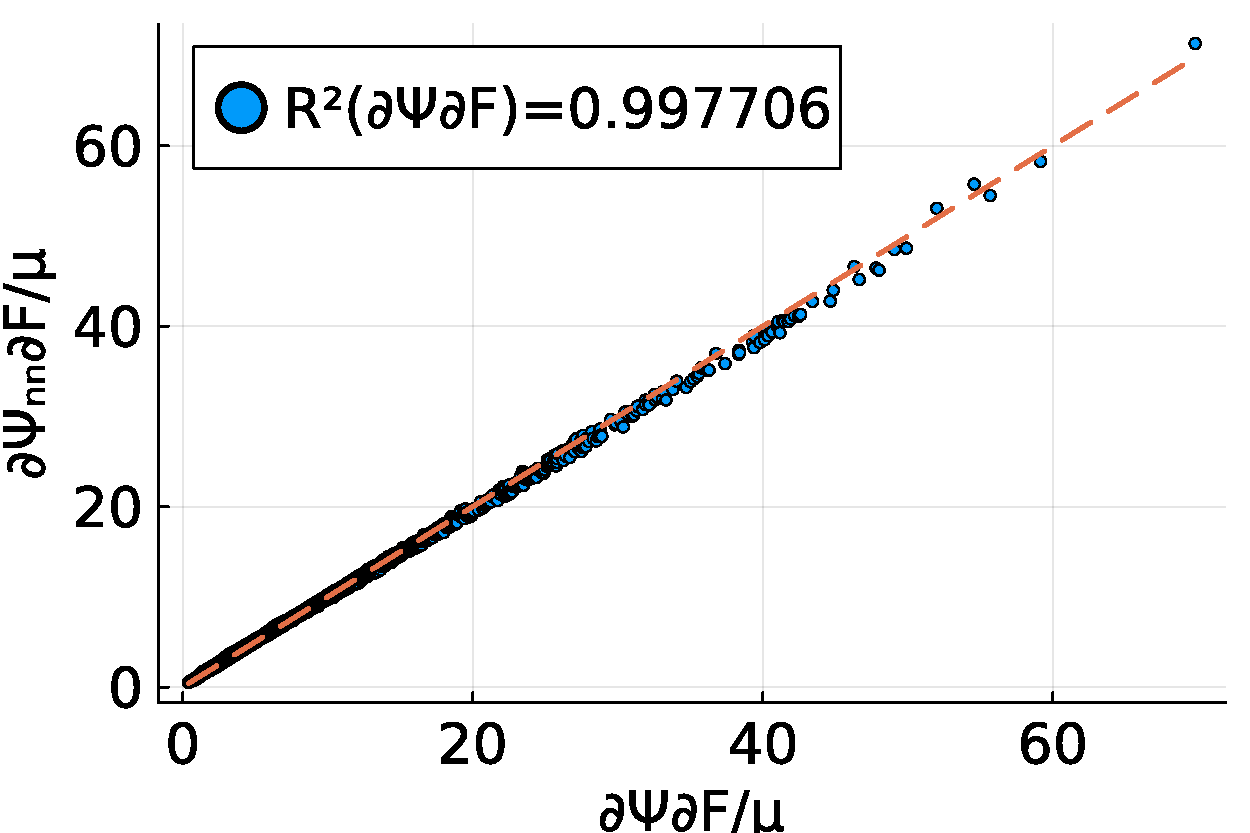
\includegraphics[width=0.3\textwidth]{Figures/ModelsStudy/_MooneyRivlin_ID_E0_P_CorrelationTest} &
		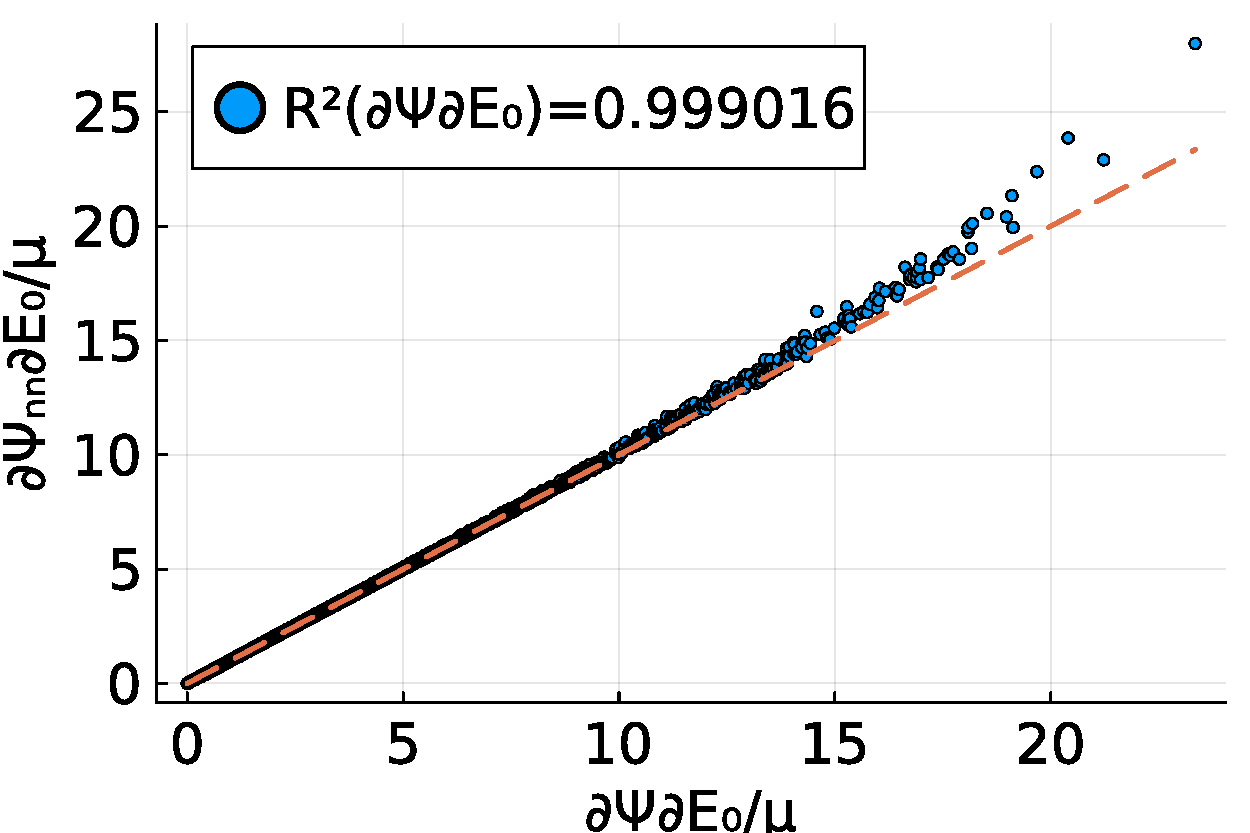
\includegraphics[width=0.3\textwidth]{Figures/ModelsStudy/_MooneyRivlin_ID_E0_E0_CorrelationTest} &
		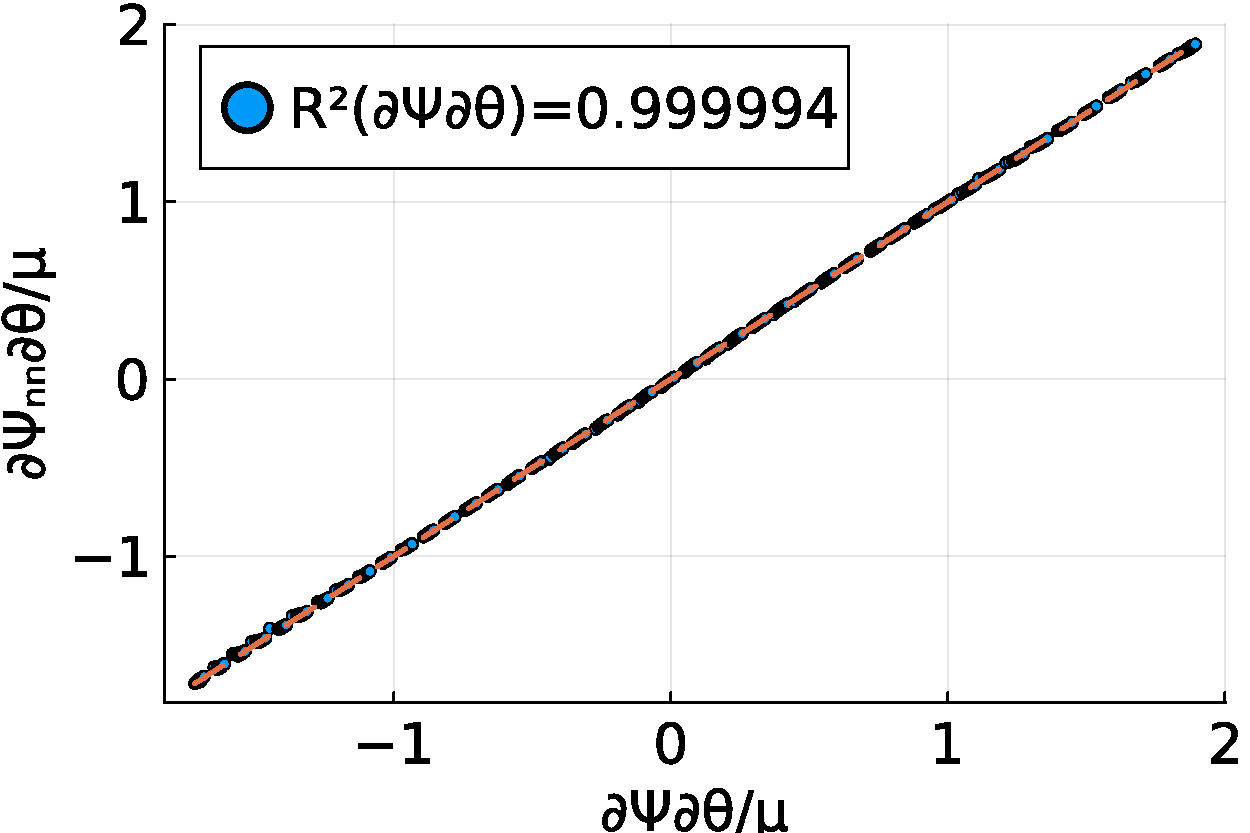
\includegraphics[width=0.3\textwidth]{Figures/ModelsStudy/_MooneyRivlin_ID_E0_theta_CorrelationTest} \\
		%
	\rotatebox{90}{\,\,\,\,\,\,\,\,\,\,\textcolor{red}{\textbf{QMR}}/\textcolor{blue}{\textbf{ID}}} &	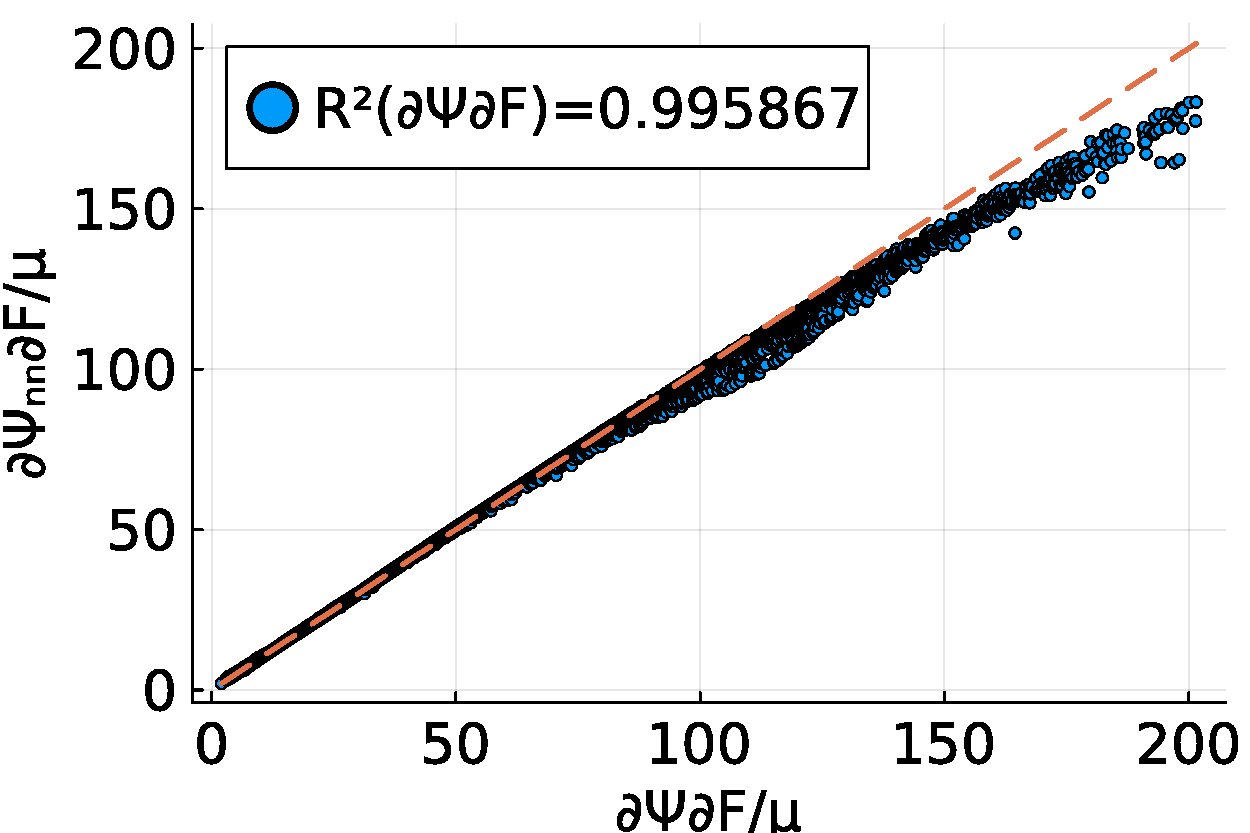
\includegraphics[width=0.3\textwidth]{Figures/ModelsStudy/_QuadraticMooneyRivlin_ID_E0_P_CorrelationTest} &
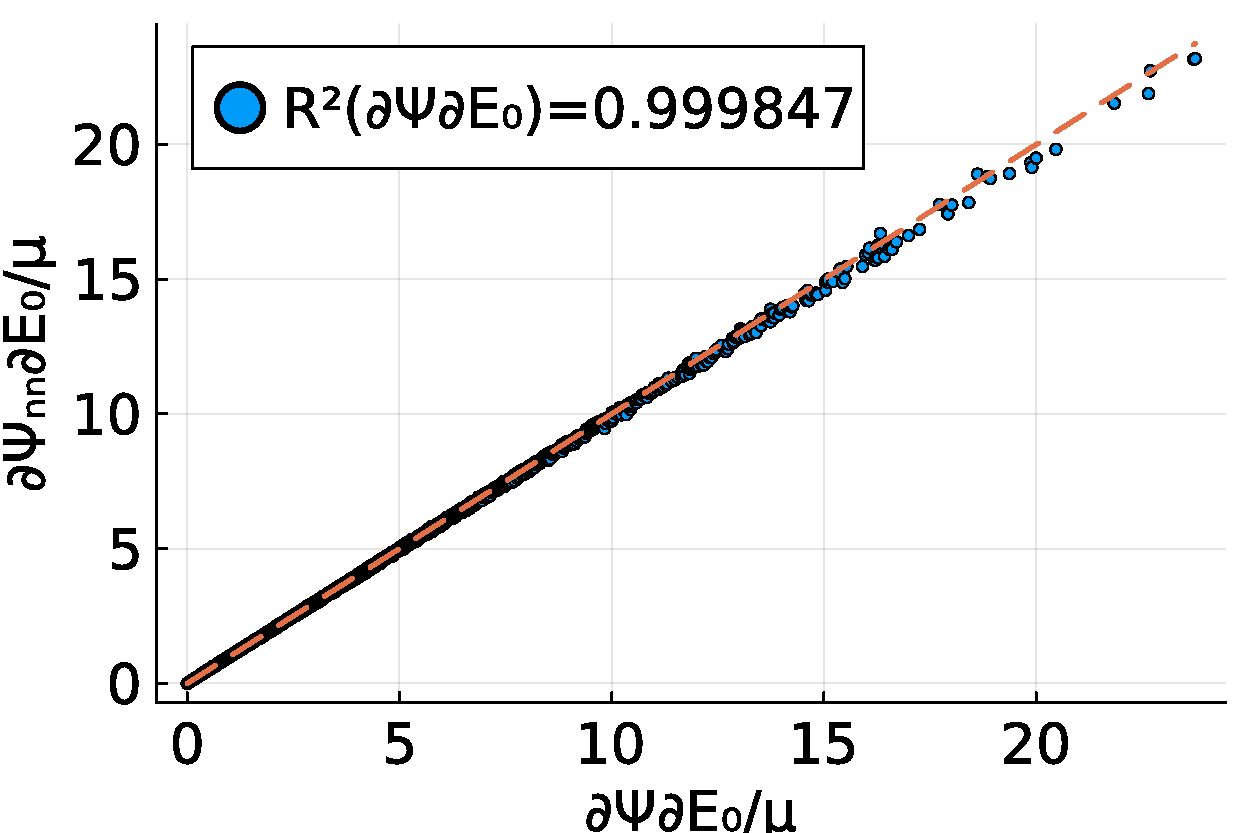
\includegraphics[width=0.3\textwidth]{Figures/ModelsStudy/_QuadraticMooneyRivlin_ID_E0_E0_CorrelationTest} &
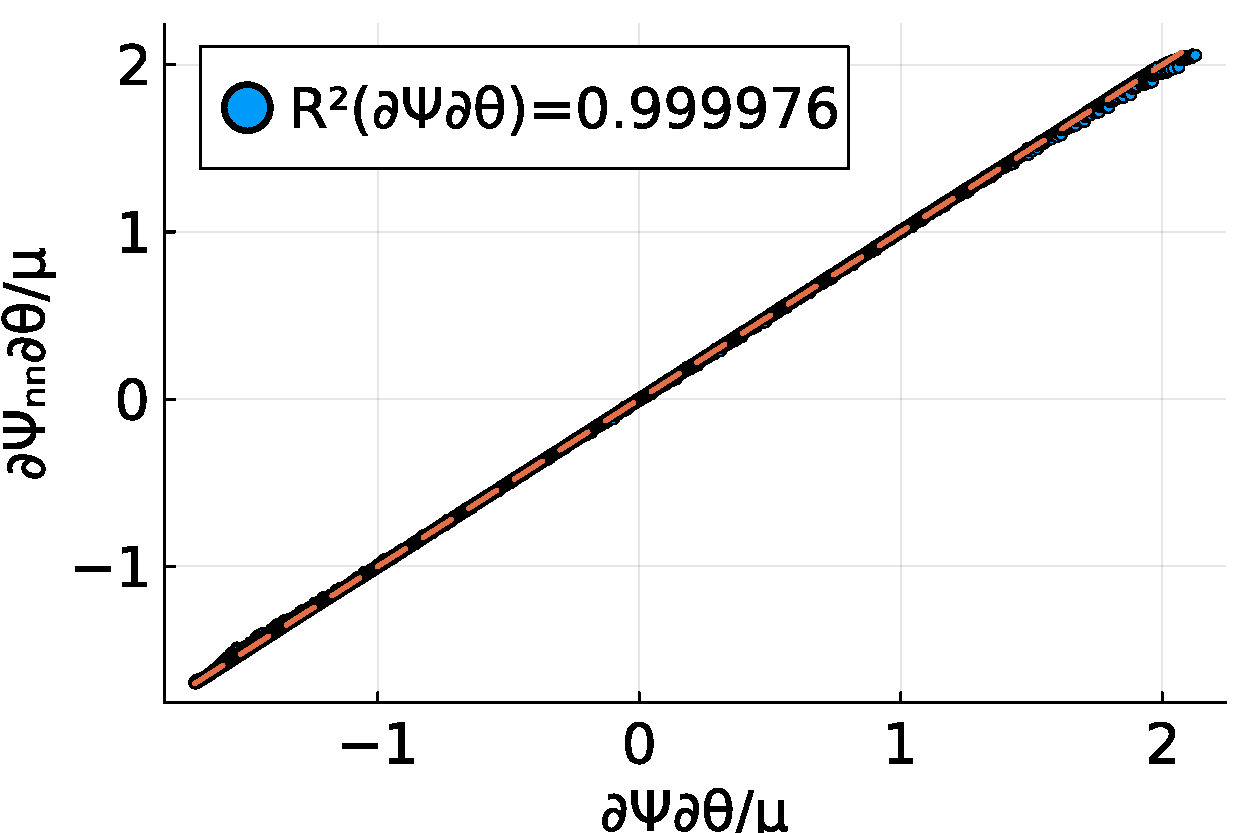
\includegraphics[width=0.3\textwidth]{Figures/ModelsStudy/_QuadraticMooneyRivlin_ID_E0_theta_CorrelationTest} \\
%
%
	\rotatebox{90}{\,\,\,\,\,\,\,\,\,\,\textcolor{red}{\textbf{Y}}/\textcolor{blue}{\textbf{ID}}}  &		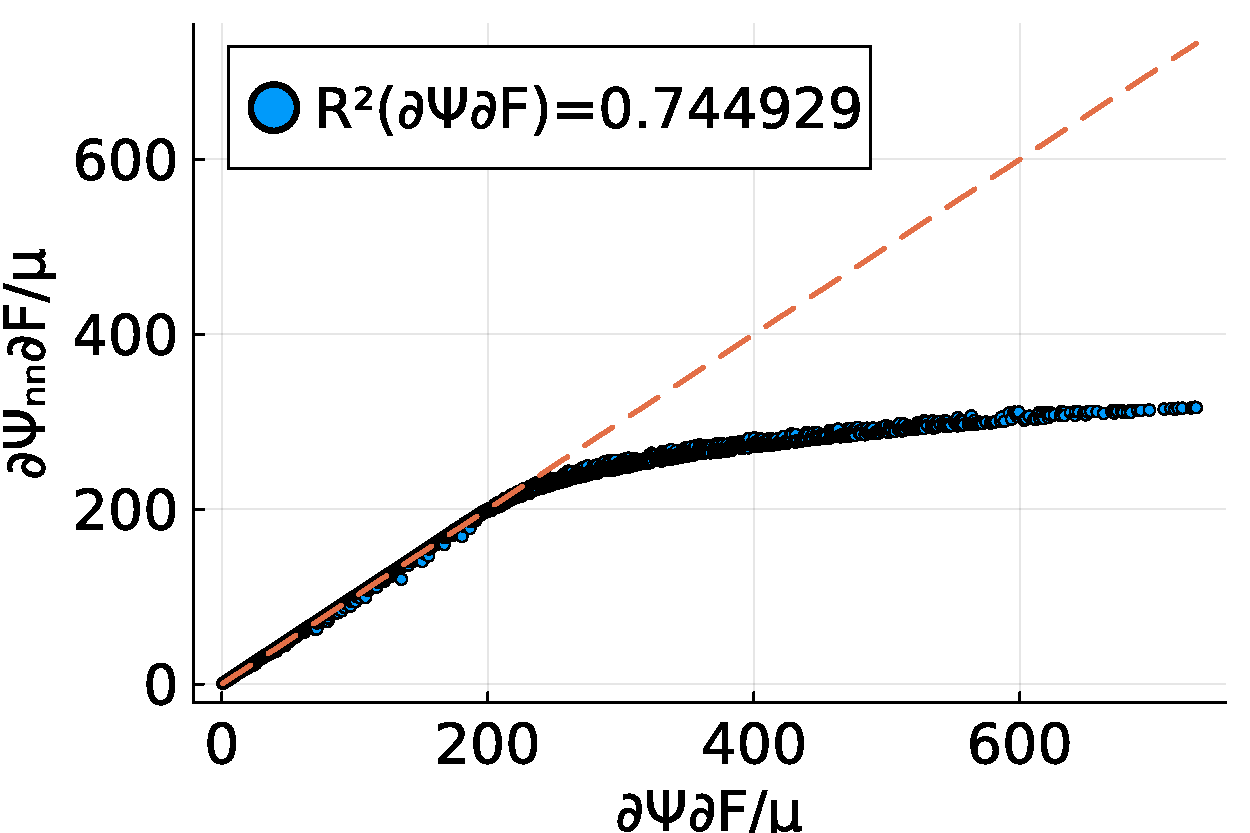
\includegraphics[width=0.3\textwidth]{Figures/ModelsStudy/_Yeoh_ID_E0_P_CorrelationTest} &
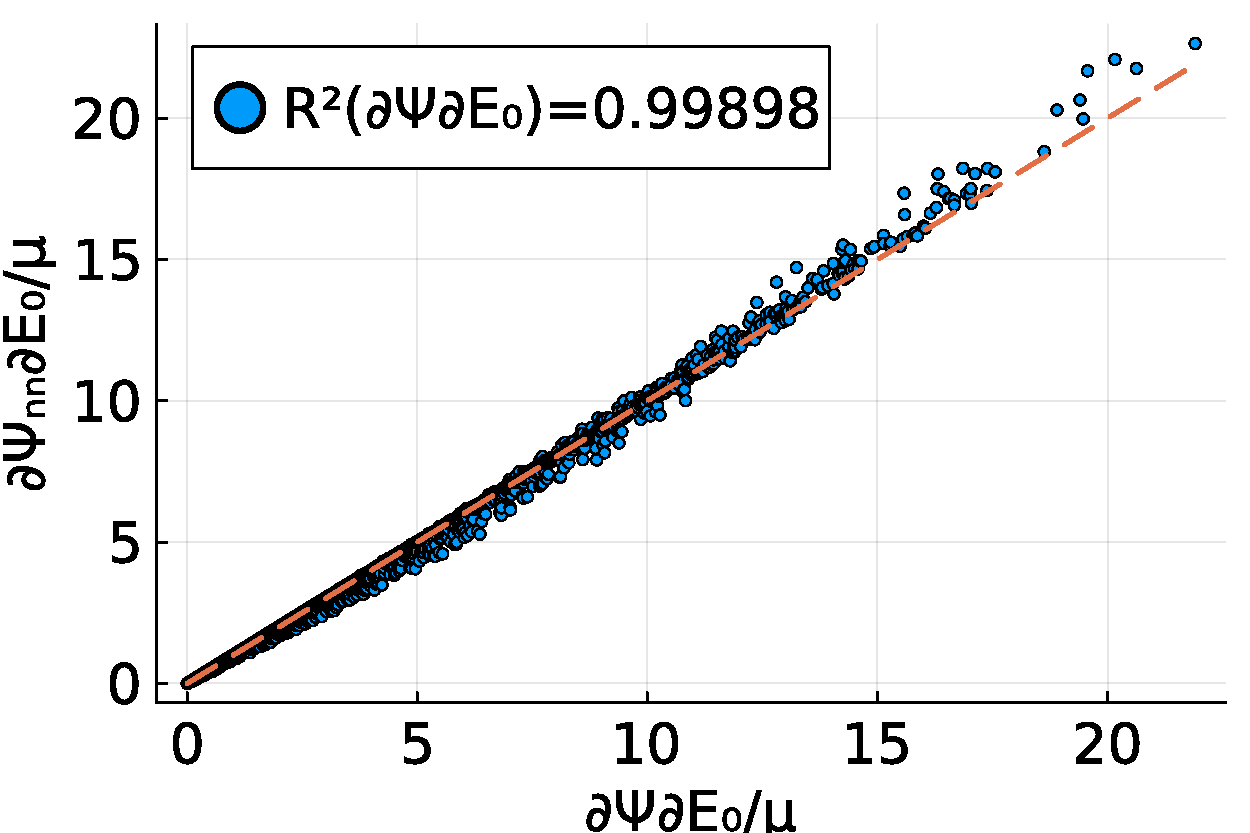
\includegraphics[width=0.3\textwidth]{Figures/ModelsStudy/_Yeoh_ID_E0_E0_CorrelationTest} &
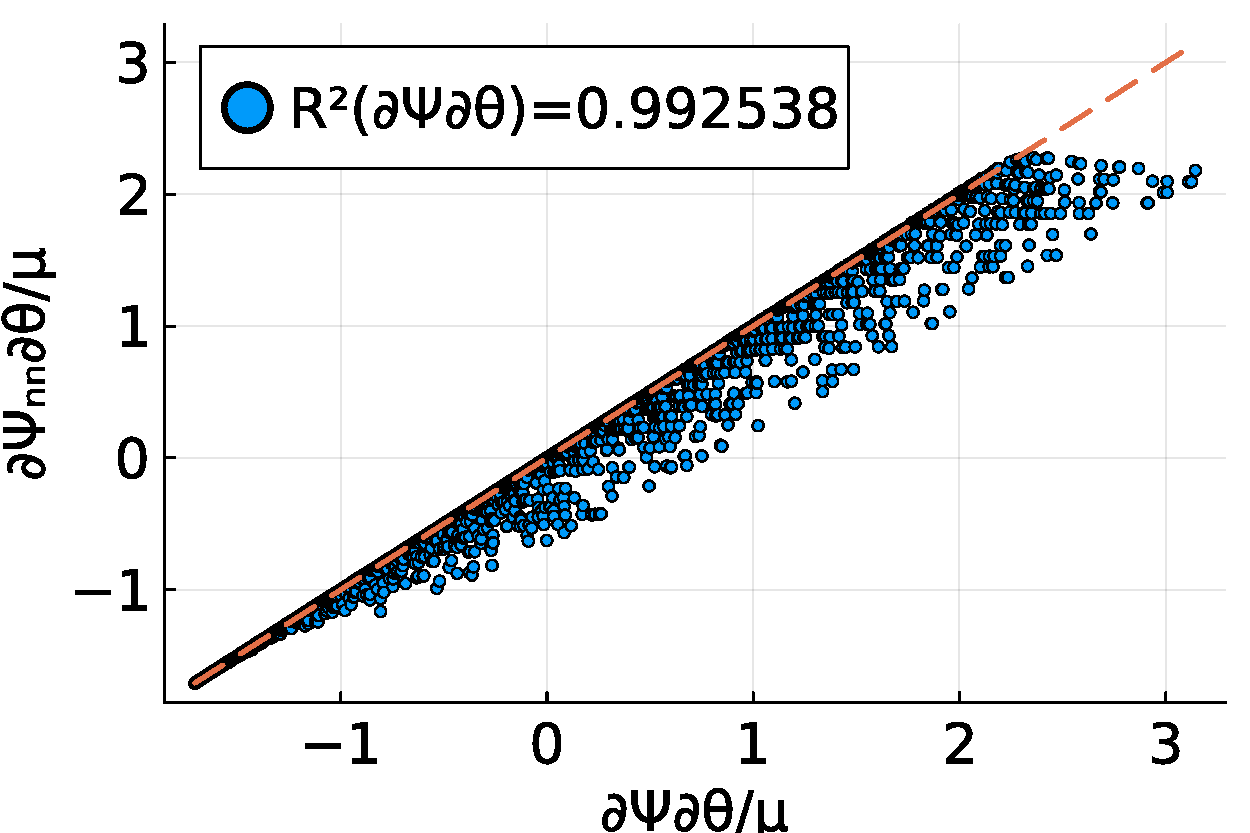
\includegraphics[width=0.3\textwidth]{Figures/ModelsStudy/_Yeoh_ID_E0_theta_CorrelationTest} \\
%
%
	\rotatebox{90}{\,\,\,\,\,\,\,\,\,\,\textcolor{red}{\textbf{G}}/\textcolor{blue}{\textbf{ID}}}  &		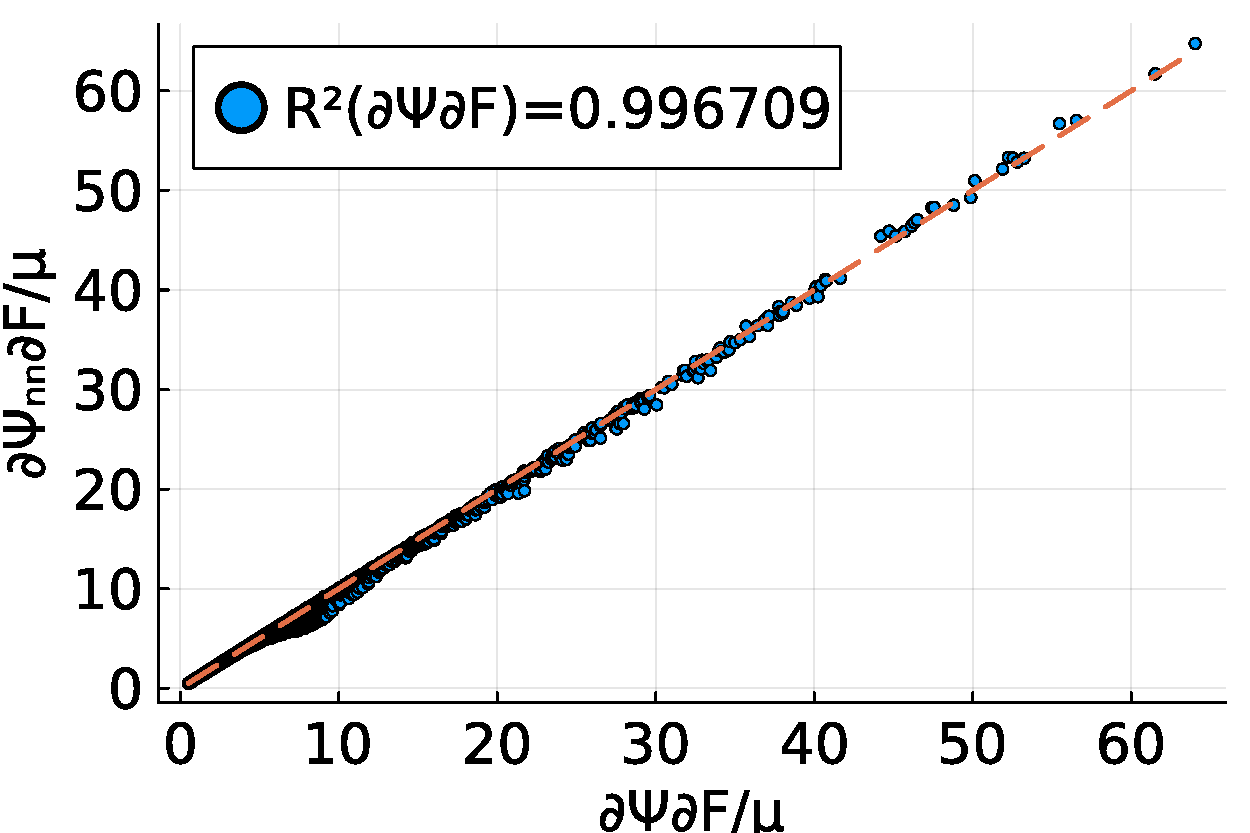
\includegraphics[width=0.3\textwidth]{Figures/ModelsStudy/_Gent_ID_E0_P_CorrelationTest} &
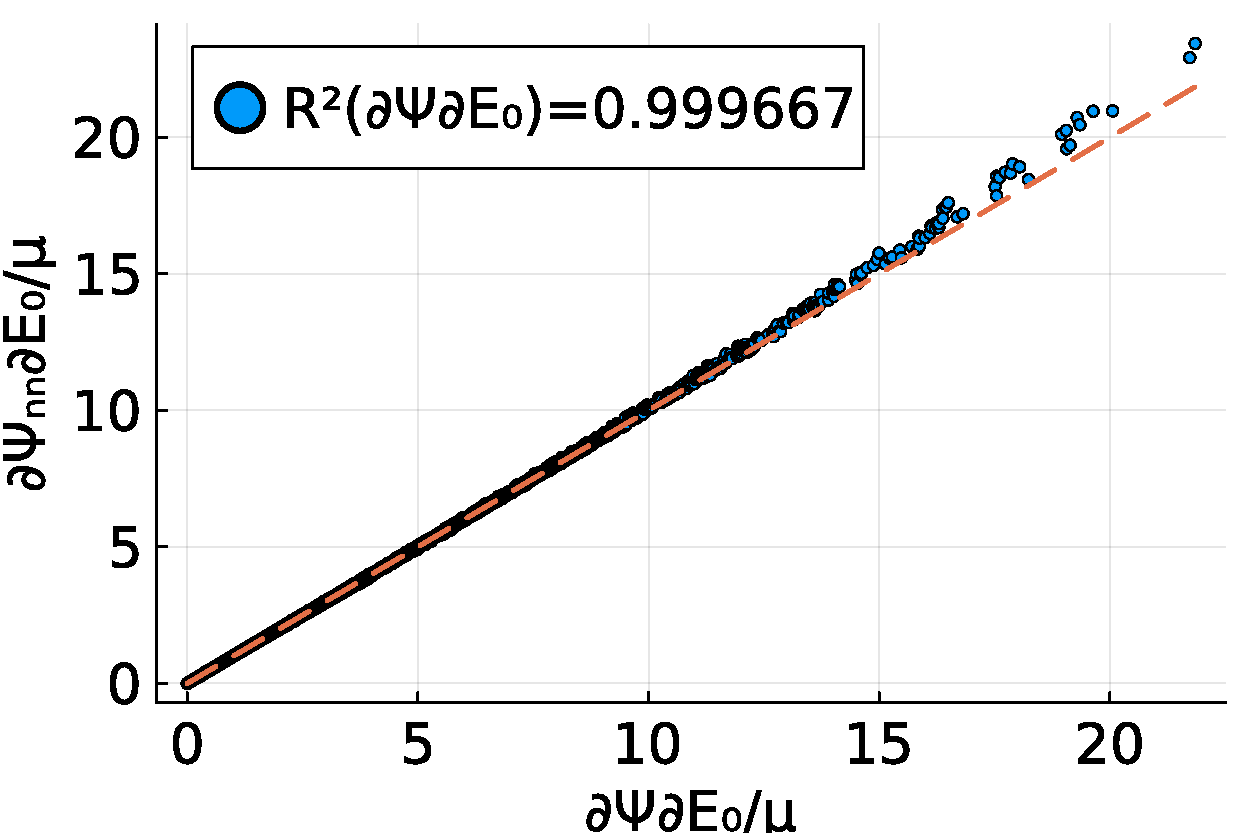
\includegraphics[width=0.3\textwidth]{Figures/ModelsStudy/_Gent_ID_E0_E0_CorrelationTest} &
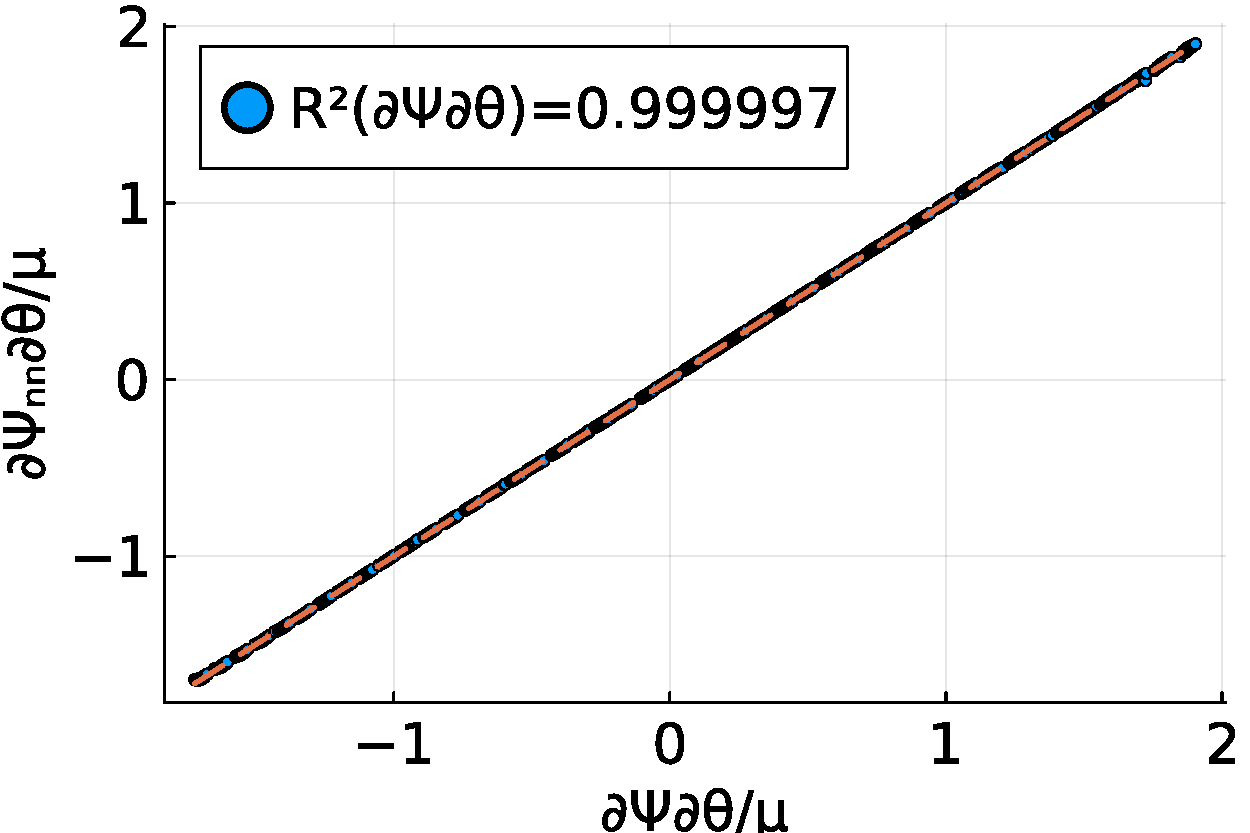
\includegraphics[width=0.3\textwidth]{Figures/ModelsStudy/_Gent_ID_E0_theta_CorrelationTest} \\
%
%
	\rotatebox{90}{\,\,\,\,\,\,\,\,\,\,\textcolor{red}{\textbf{TI}}/\textcolor{blue}{\textbf{ID}}}  &		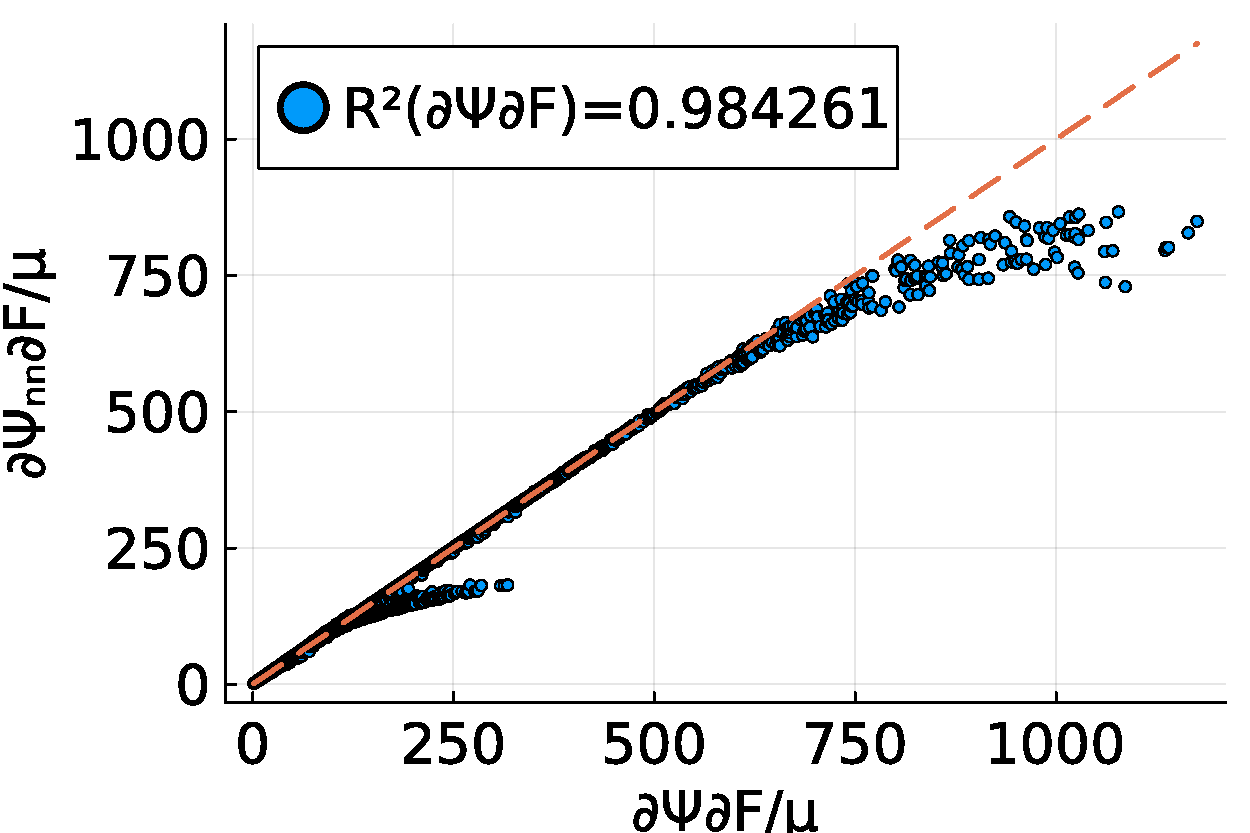
\includegraphics[width=0.3\textwidth]{Figures/ModelsStudy/_TI_ID_E0_P_CorrelationTest} &
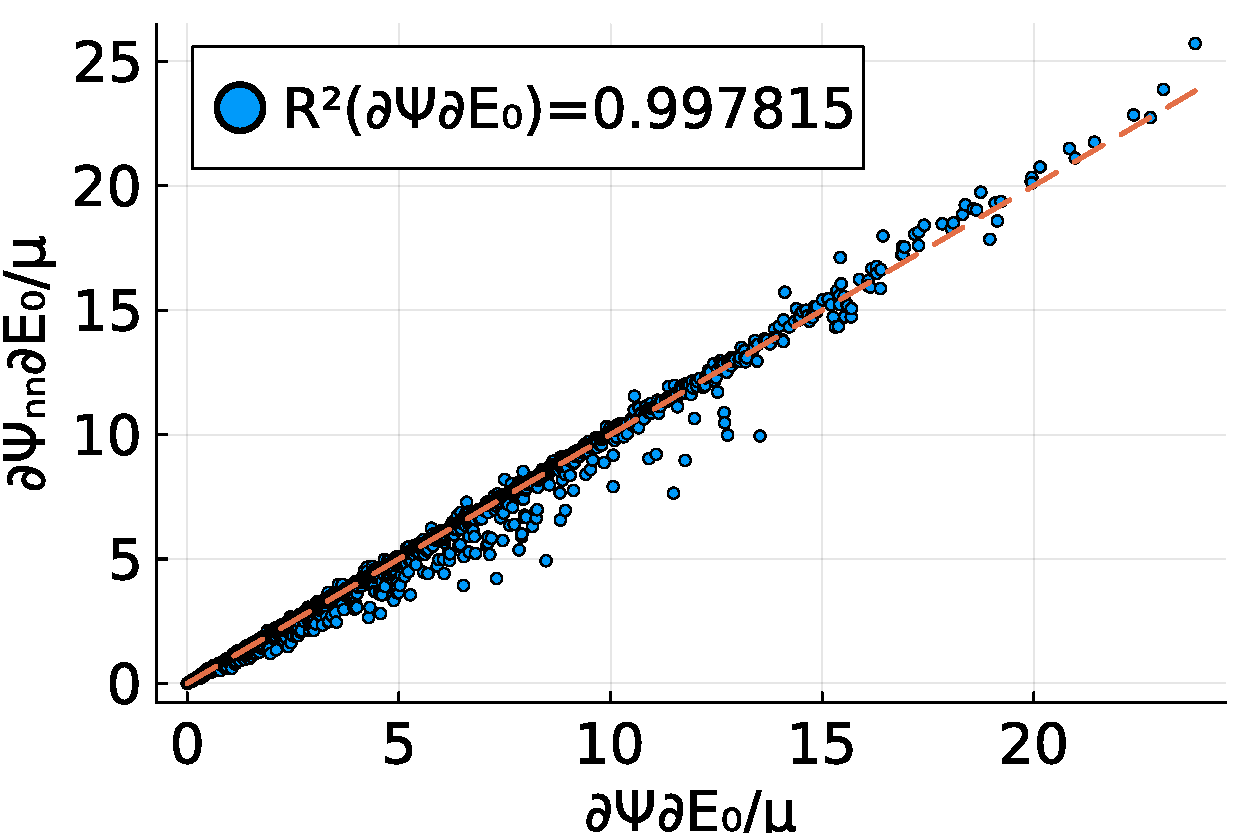
\includegraphics[width=0.3\textwidth]{Figures/ModelsStudy/_TI_ID_E0_E0_CorrelationTest} &
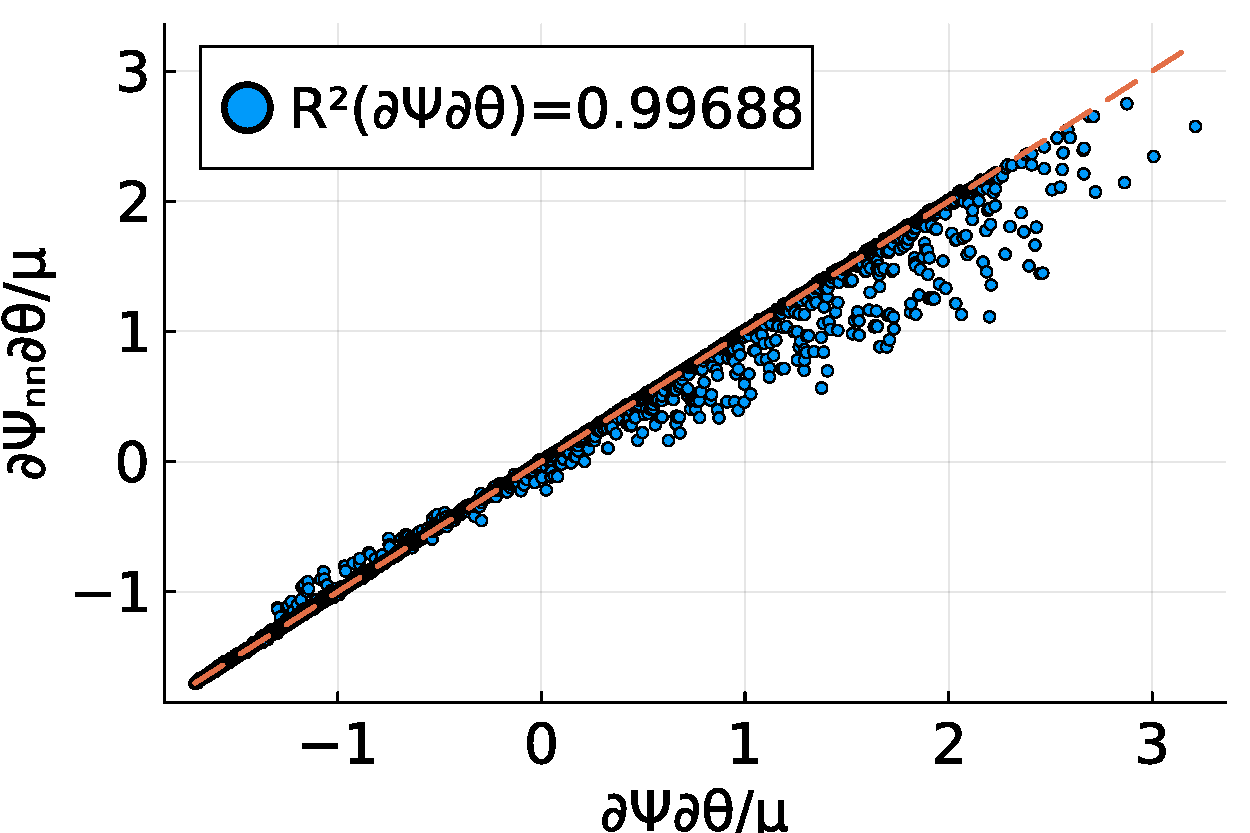
\includegraphics[width=0.3\textwidth]{Figures/ModelsStudy/_TI_ID_E0_theta_CorrelationTest} \\
%
%
	\rotatebox{90}{\,\,\,\,\,\,\,\,\,\,\textcolor{red}{\textbf{MR}}/\textcolor{blue}{\textbf{ES}}}  &	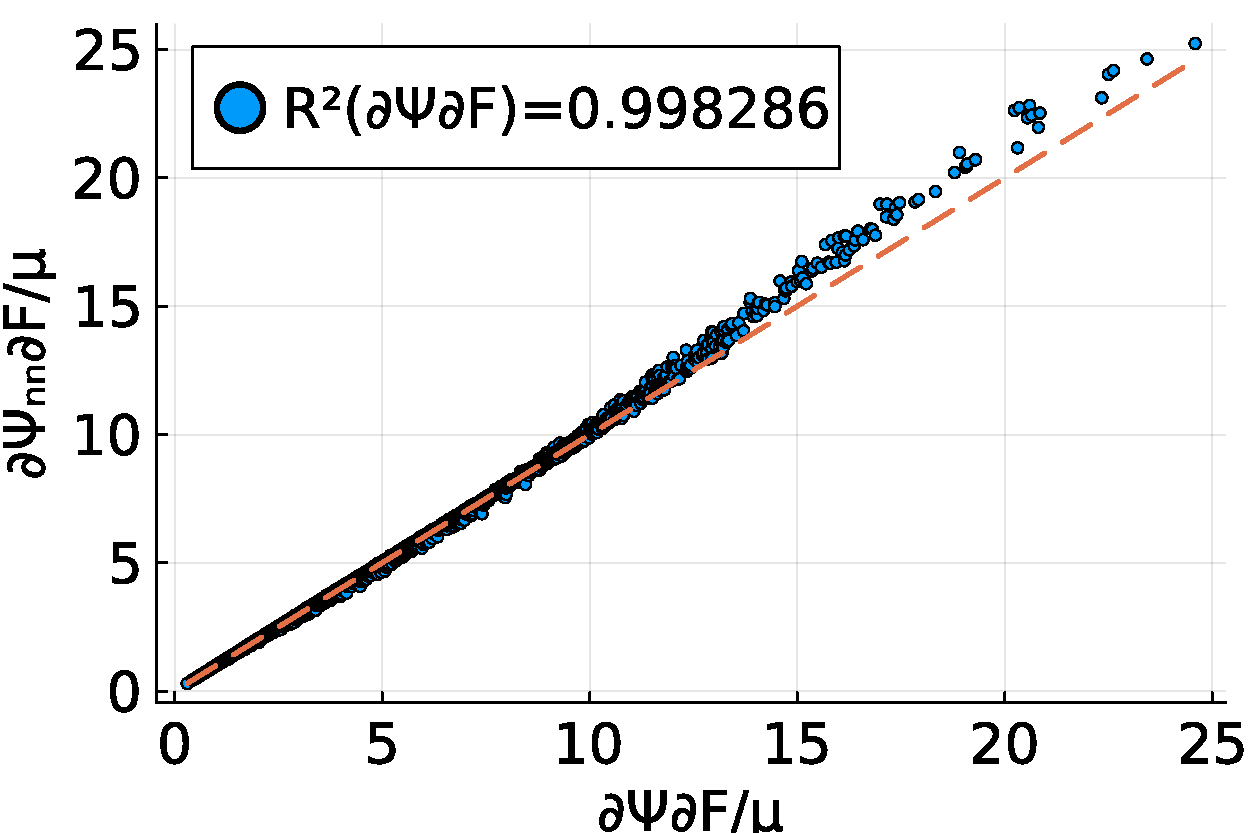
\includegraphics[width=0.3\textwidth]{Figures/ModelsStudy/_MooneyRivlin_ElectricSaturation_P_CorrelationTest} &
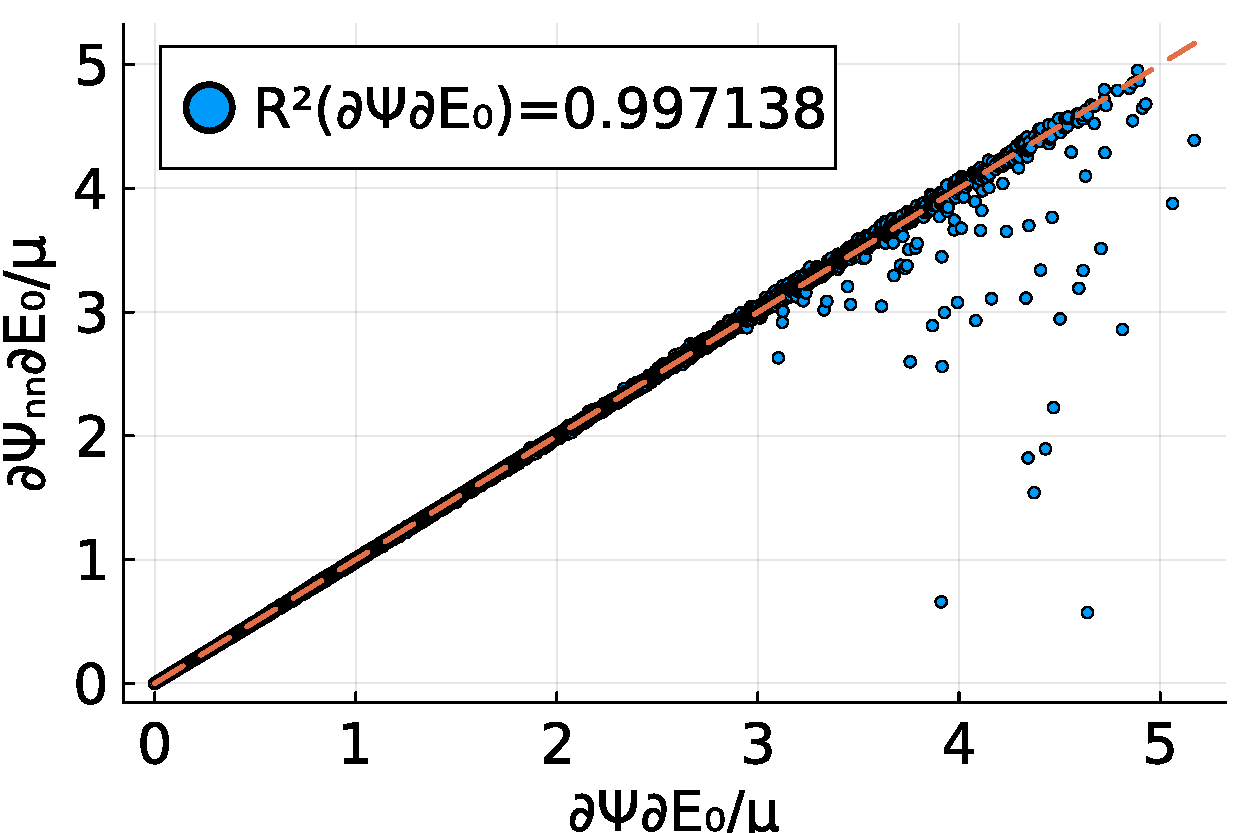
\includegraphics[width=0.3\textwidth]{Figures/ModelsStudy/_MooneyRivlin_ElectricSaturation_E0_CorrelationTest} &
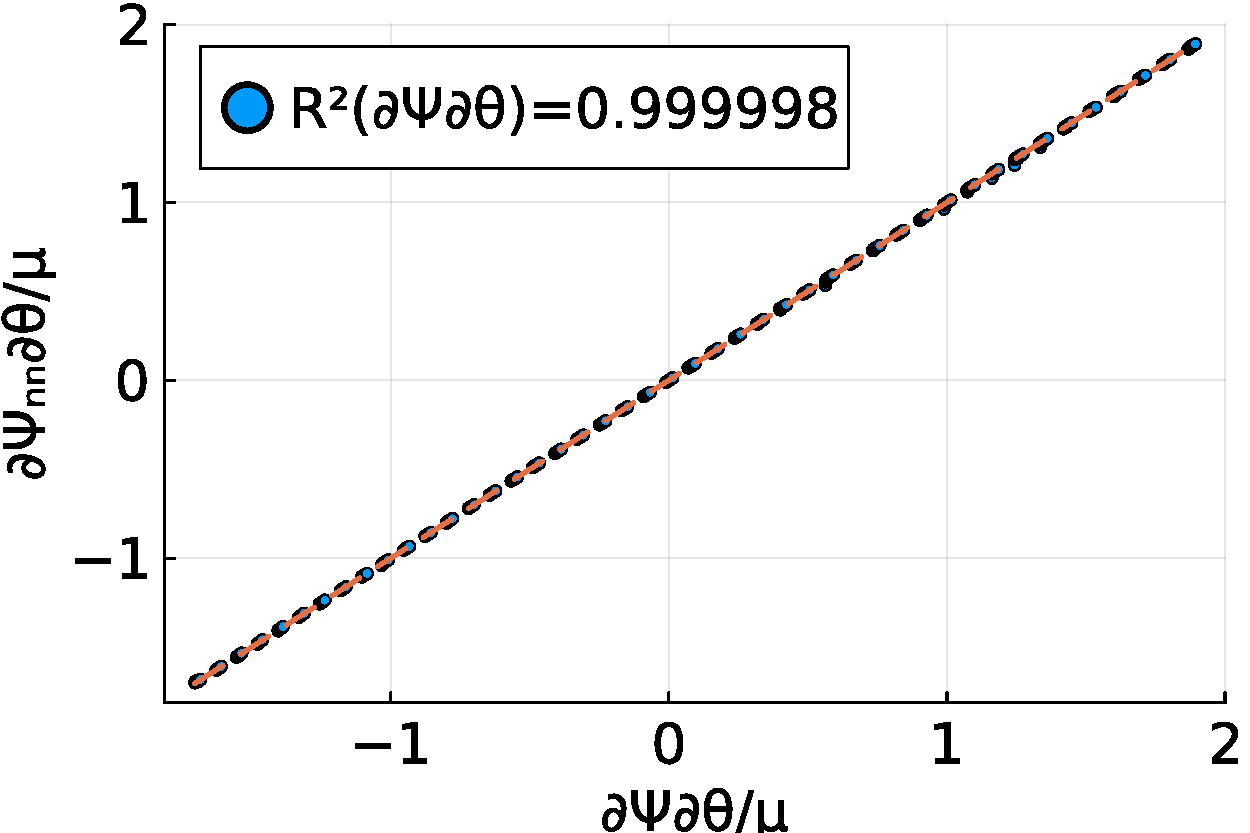
\includegraphics[width=0.3\textwidth]{Figures/ModelsStudy/_MooneyRivlin_ElectricSaturation_theta_CorrelationTest} \\
%
%
	\end{tabular}
	%
	%		\includegraphics[width=0.4\textwidth]{pictures_paper/inkscape_pictures/template_example_3.pdf}
	\caption{\textbf{Calibration Strategy 1}. Correlation of prediction $\{\partial_{\vect{F}}\Psi_{nn},\partial_{\vect{E}_0}\Psi_{nn},\partial_{\theta}\Psi_{nn}\}$ and testing data $\{\partial_{\vect{F}}\Psi,\partial_{\vect{E}_0}\Psi,\partial_{\theta}\Psi\}$ using the purely mechanical (in red) and electro-mechanical (in blue) contributions of the ground truth Helmholtz strain energy model used for the calibration. The training data represents a subset of the testing data containing the $20\%$ of the data in the latter. In all cases we have considered an architecture of $4$ layers and $8$ neurons per layer.}
	\label{fig:correlation strategy 1}
\end{figure}

















We conducted additional testing of the calibrated models in scenarios beyond those included in the training set. It is important to note that both the training and testing sets were generated using a similar in-silico data generation strategy, as outlined in Section \ref{sec:data generation strategy 1} and based on the methodology of \cite{OKunc_19_01}. Our objective is to further evaluate the calibrated potentials using a distinct data generation strategy, in which the deformation gradient tensor and the electric field are defined according to
%
\begin{equation}\label{eqn:experiments}
	\vect{F}=\begin{bmatrix}
		\lambda & \gamma & 0\\
		0&\lambda & 0\\
		0  &  0 & 1/\lambda^2
	\end{bmatrix};\,\,1\leq \lambda \leq 1.8; \qquad \vect{E}_0 =  \begin{bmatrix}
	\alpha  \\  \alpha  \\  0
\end{bmatrix}\,\,0\leq \alpha\leq 1.5\sqrt{\frac{\mu}{\varepsilon}}
\end{equation}

The objective is to assess the agreement between the derivatives of the calibrated model, $\Psi_{nn}(\vect{F}, \vect{E}0, \theta)$, and those of the ground truth model across various temperature values for the specified experimental setup. Figure \ref{fig:physical experiments} illustrates this comparison, focusing on the neural network-based potential $\Psi_{nn}(\vect{F}, \vect{E}_0, \theta)$ and a single ground truth constitutive model. The figure demonstrates a remarkable alignment between the calibrated and ground truth models, highlighting the calibrated model's capacity to accurately predict the ground truth response, even in scenarios outside its training domain.



\begin{figure}[hbtp]
	\centering
	\begin{tabular}{cc}
		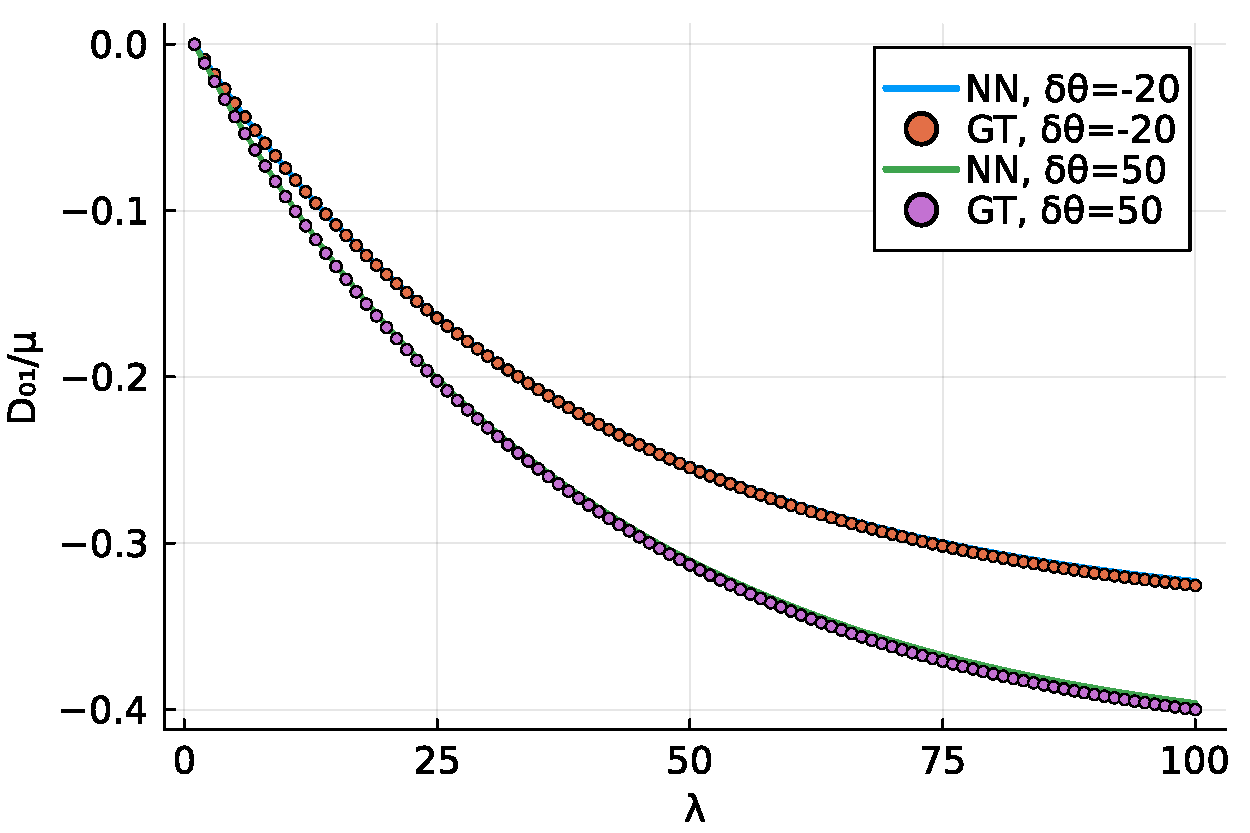
\includegraphics[width=0.4\textwidth]{Figures/PotentialStudy/_PhysicalExperiments_MooneyRivlin_ID_E0_D1} &
		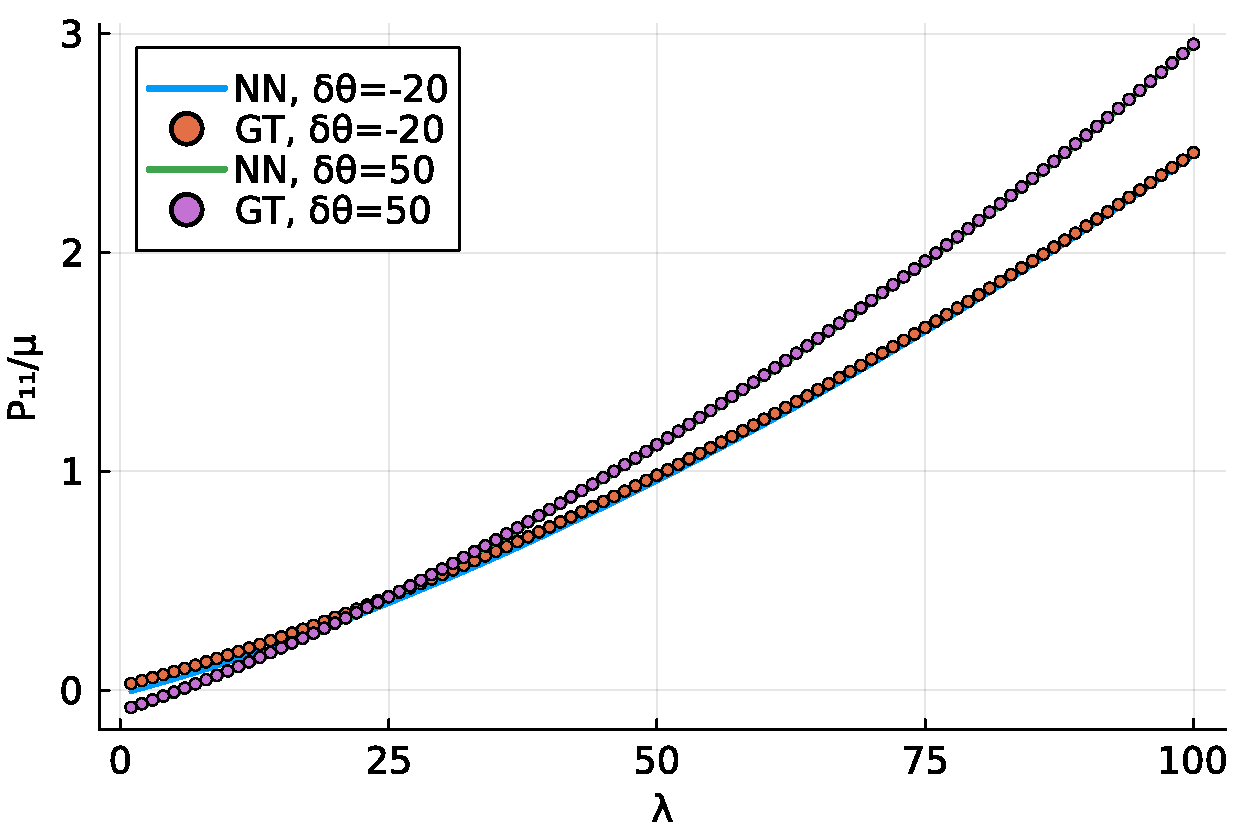
\includegraphics[width=0.4\textwidth]{Figures/PotentialStudy/_PhysicalExperiments_MooneyRivlin_ID_E0_F11}  \\
		(a)  &  (b)\\
		%
		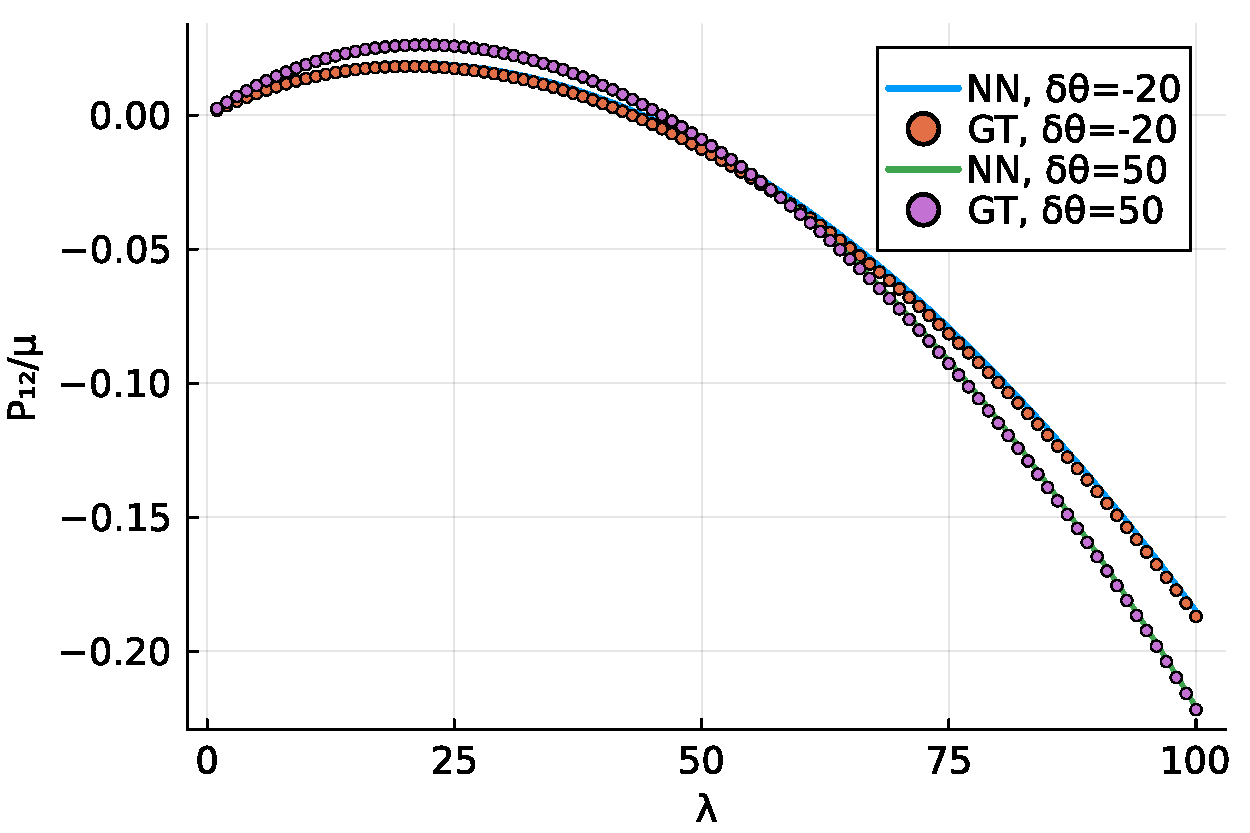
\includegraphics[width=0.4\textwidth]{Figures/PotentialStudy/_PhysicalExperiments_MooneyRivlin_ID_E0_F12} &
		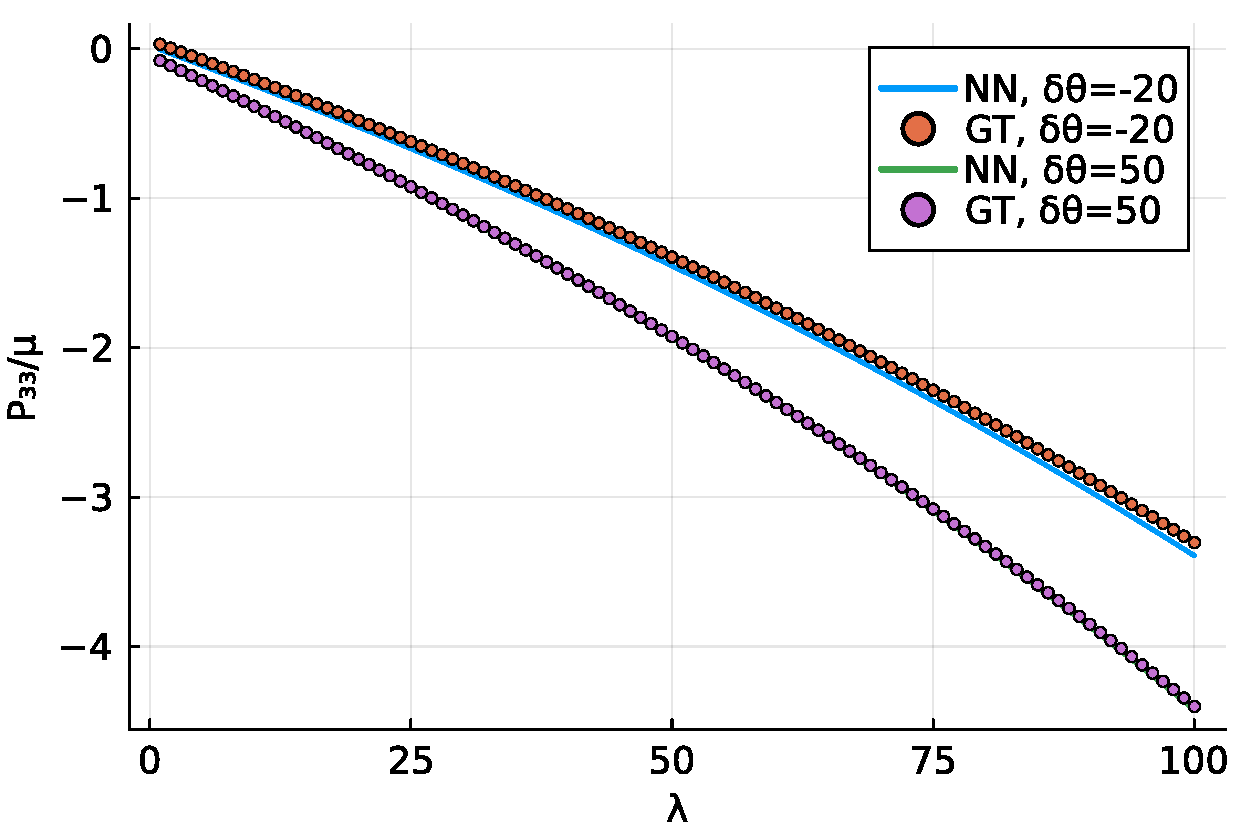
\includegraphics[width=0.4\textwidth]{Figures/PotentialStudy/_PhysicalExperiments_MooneyRivlin_ID_E0_F33}  \\
		(c)  &  (d)		
	\end{tabular}
	%
	%		\includegraphics[width=0.4\textwidth]{pictures_paper/inkscape_pictures/template_example_3.pdf}
	\caption{\textbf{Calibration Strategy 1}. Prediction of calibrated model $\Psi_{nn}(\vect{F}, \vect{E}_0, \theta)$ and ground truth model across various temperature values for the experimental setup in \eqref{eqn:experiments}. The ground truth model $\Psi(\vect{F},\vect{E}_0,\theta)$ considers a Mooney-Rivlin model for the mechanical contribution, i.e. $Psi_{m}$ and an ideal dielectric model for the electro-mechanical contribution, i.e. $\Psi_{em}$.}
	\label{fig:physical experiments}
\end{figure}


\subsubsection{Generalization results for all the thermodynamical potentials}

In the previous section, we focused exclusively on the calibration of Helmholtz-type neural network-based potentials, specifically $\Psi_{nn}(\vect{F},\vect{E}_0,\theta)$. he objective of this section, however, is to demonstrate that, while we have primarily considered a Helmholtz-type ground truth potential $\Psi(\vect{F},\vect{E}_0,\theta)$, we can successfully calibrate neural network-based potentials corresponding to alternative formulations, namely  $e_{nn}(\vect{F},\vect{D}_0,\eta)$, $\Upsilon_{nn}(\vect{F},\vect{D}_0,\theta)$ and $\Gamma_{nn}(\vect{F},\vect{E}_0,\eta)$, as outlined in Section \ref{sec:fundamentals strategy 1}. o illustrate this capability, we consider the following case:

\begin{itemize}
	\item fixed neural network architecture with 4 hidden layers and 8 neurons
	
	\item ground truth model with $\Psi_m$ corresponding with a Mooney-Rivlin model and $\Psi_{em}$ with an ideal dielectric model.
\end{itemize}

Under such scenario, Figure \ref{fig:strategy 1--the potentials} presents the correlation results for the test dataset, which is larger than the training dataset, for the four potentials, namely $\Psi_{nn}(\vect{F},\vect{E}_0,\theta)$, $e_{nn}(\vect{F},\vect{D}_0,\eta)$, $\Upsilon_{nn}(\vect{F},\vect{D}_0,\theta)$ and $\Gamma_{nn}(\vect{F},\vect{E}_0,\eta)$. The figure demonstrates an excellent agreement between the predictions made by the calibrated potentials and the ground truth model, confirming the reliability of the calibrated models in predicting the behavior of the ground truth.

\begin{figure}[hbtp]
	\centering
	\begin{tabular}{ccc}
		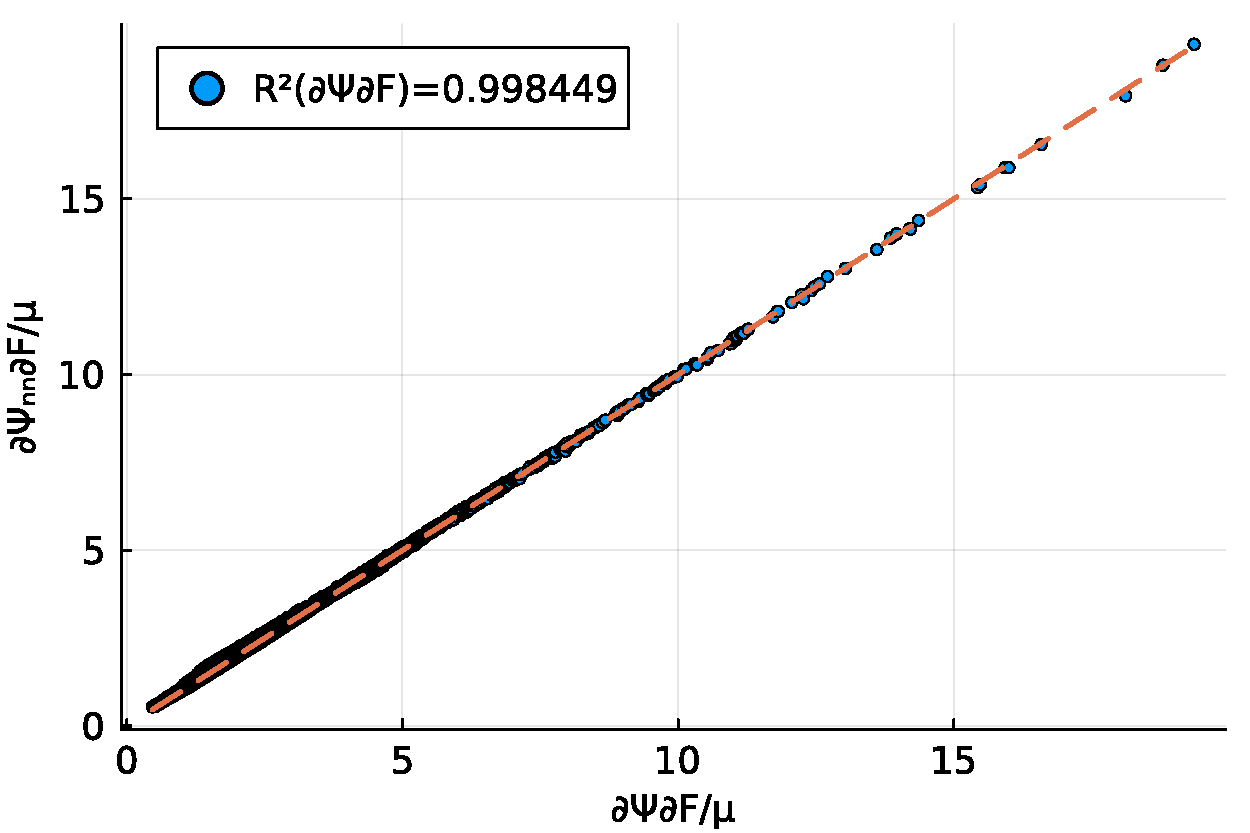
\includegraphics[width=0.33\textwidth]{Figures/PotentialStudy/Psi_P_CorrelationTest} &
		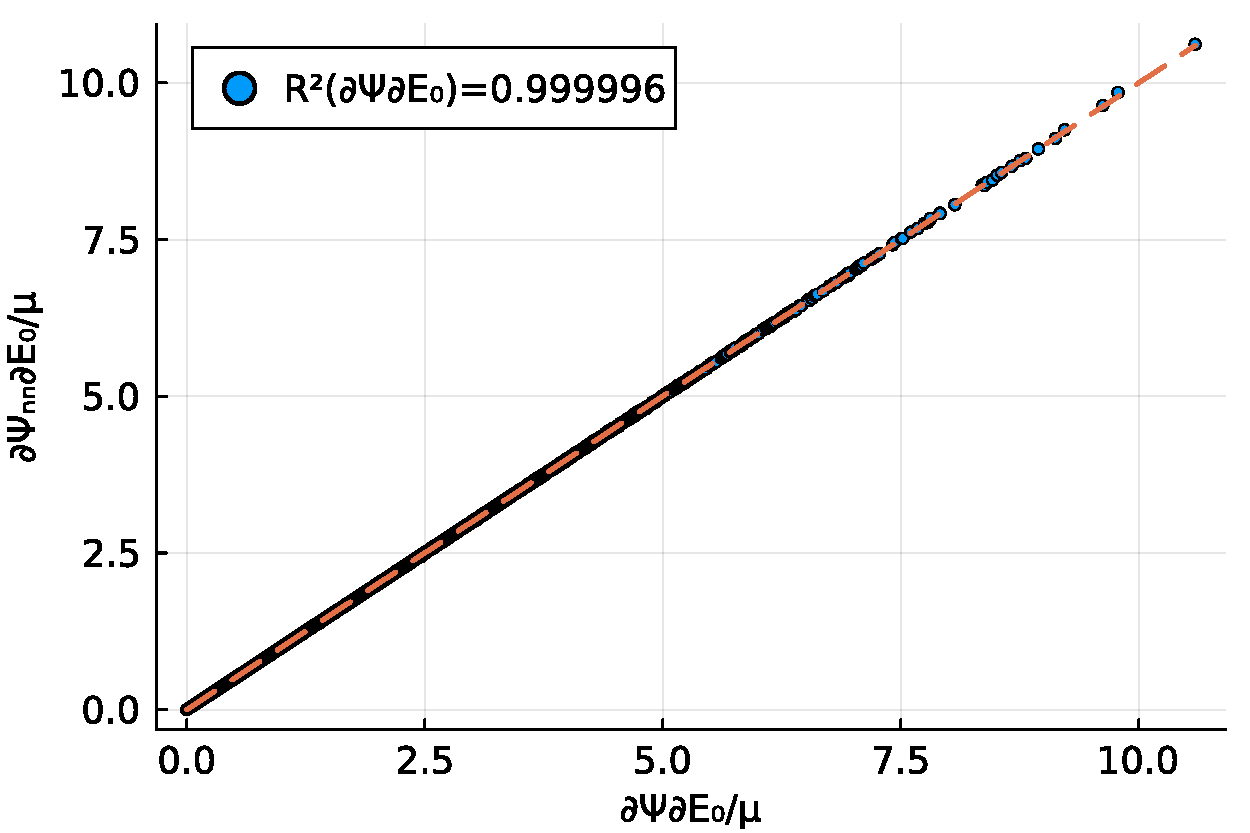
\includegraphics[width=0.33\textwidth]{Figures/PotentialStudy/Psi_E0_CorrelationTest} &
		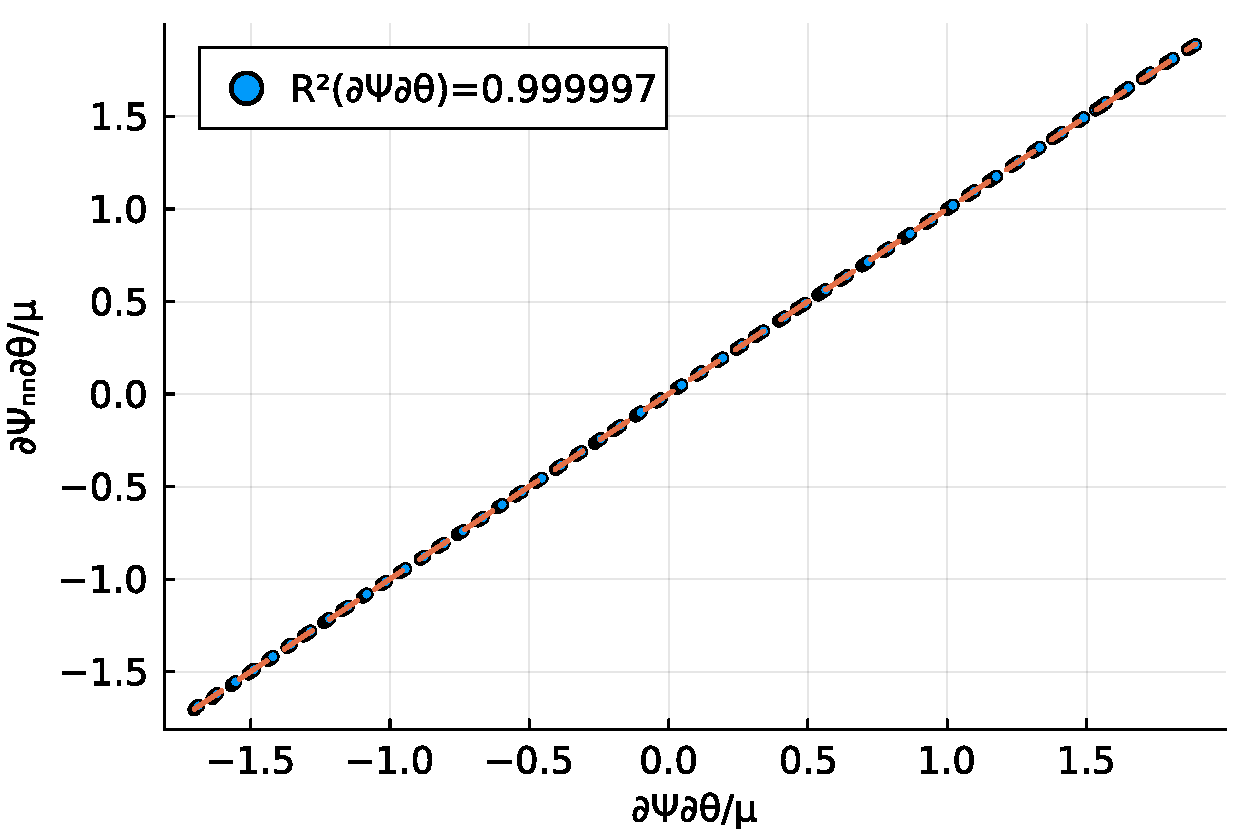
\includegraphics[width=0.33\textwidth]{Figures/PotentialStudy/Psi_theta_CorrelationTest} \\
		%
		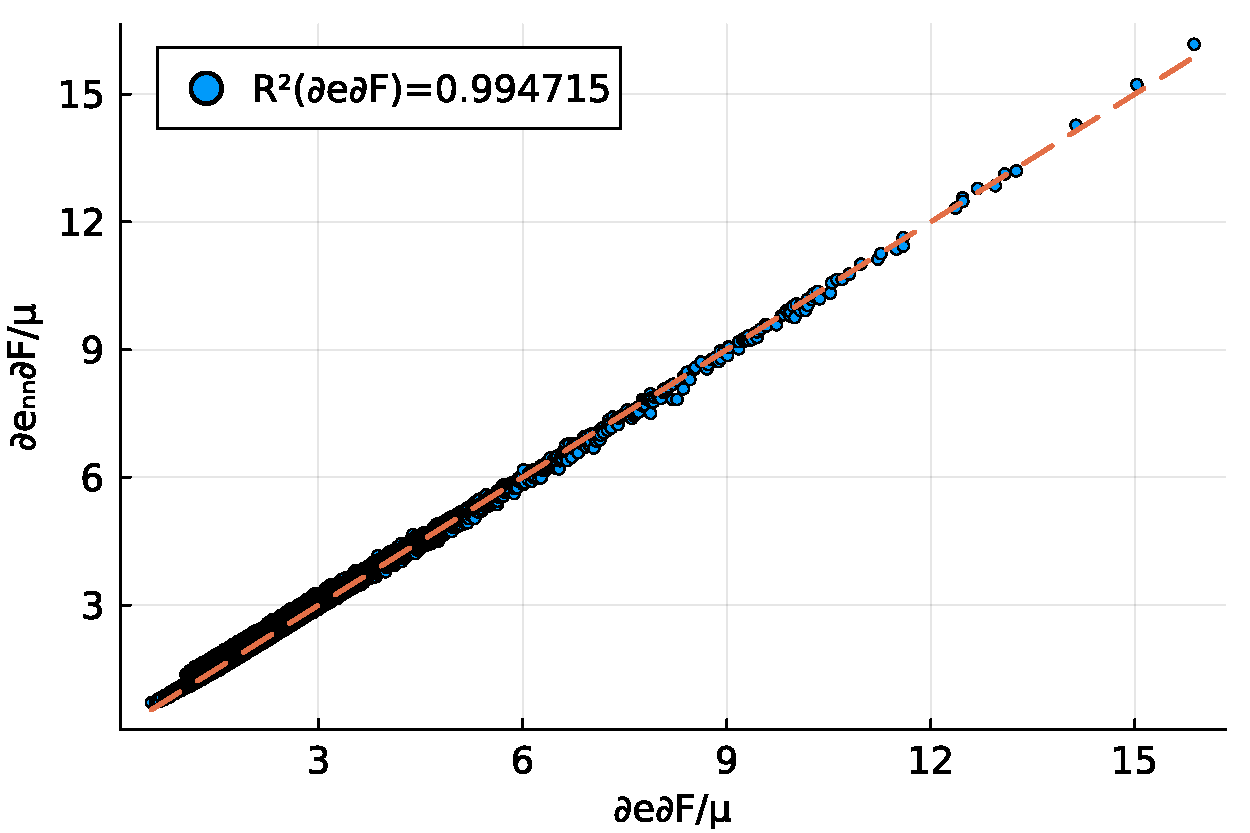
\includegraphics[width=0.33\textwidth]{Figures/PotentialStudy/e_P_CorrelationTest} &
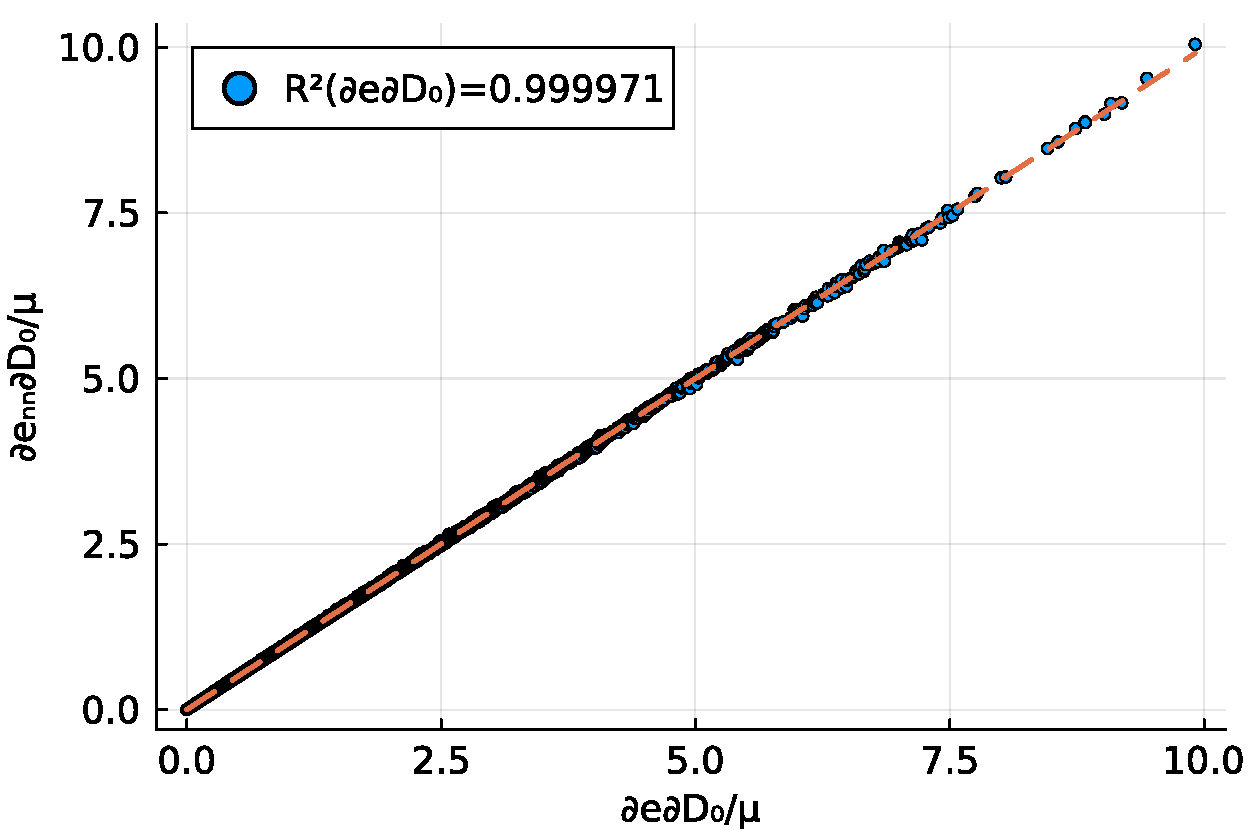
\includegraphics[width=0.33\textwidth]{Figures/PotentialStudy/e_E0_CorrelationTest} &
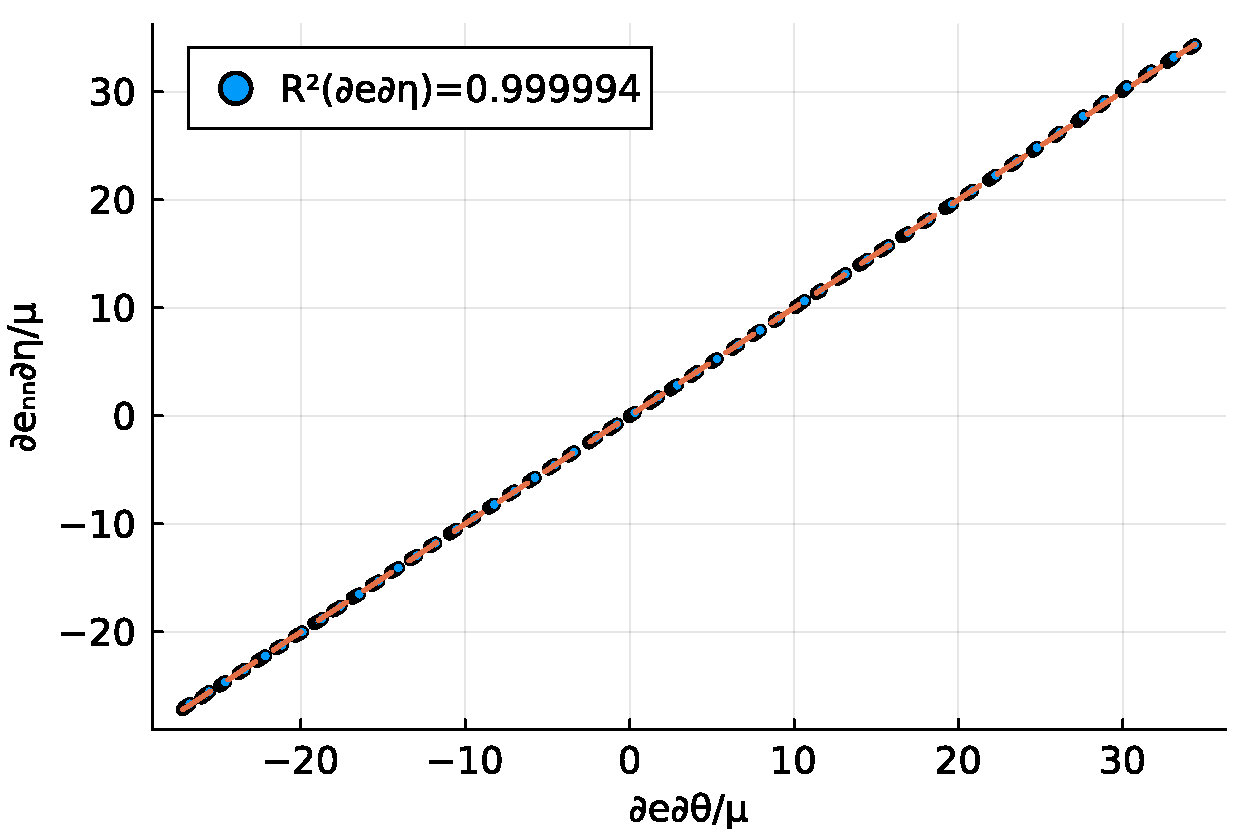
\includegraphics[width=0.33\textwidth]{Figures/PotentialStudy/e_theta_CorrelationTest} \\		%	
%	
		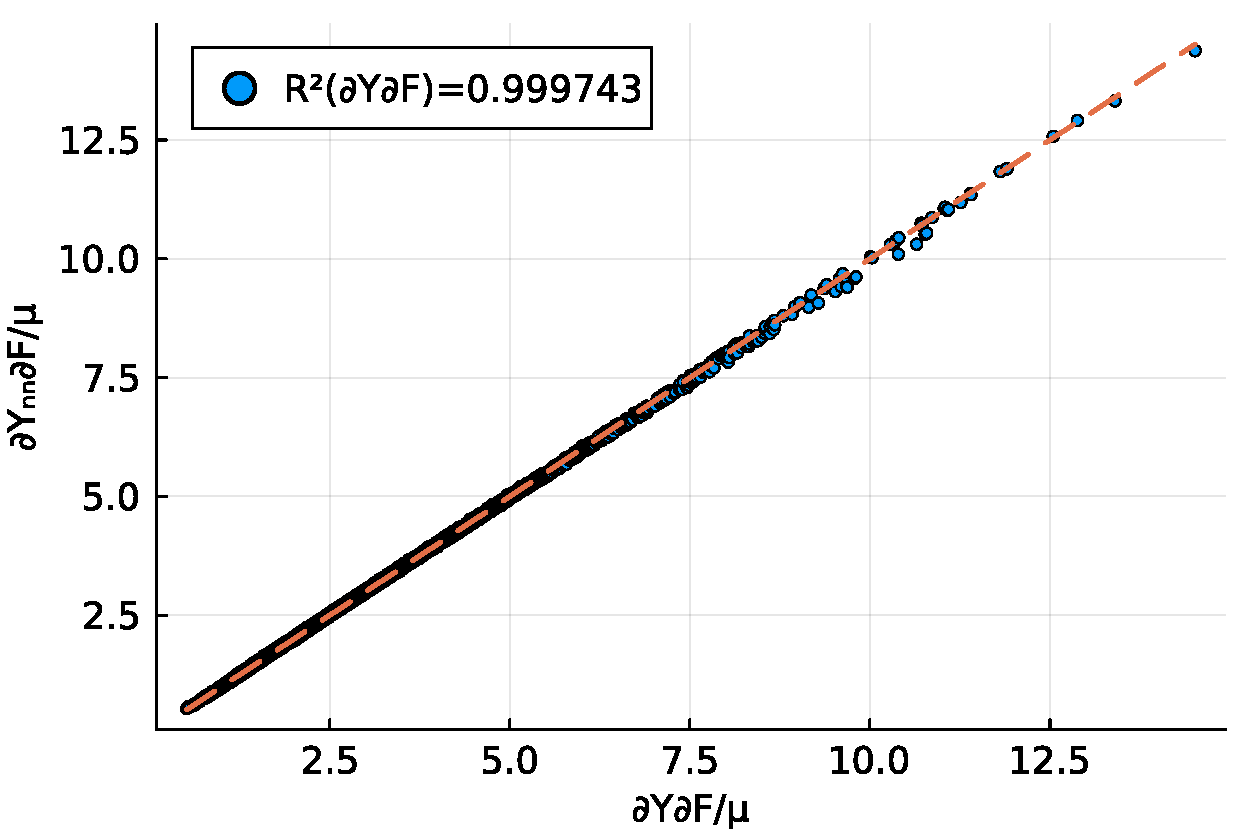
\includegraphics[width=0.33\textwidth]{Figures/PotentialStudy/Upsilon_P_CorrelationTest} &
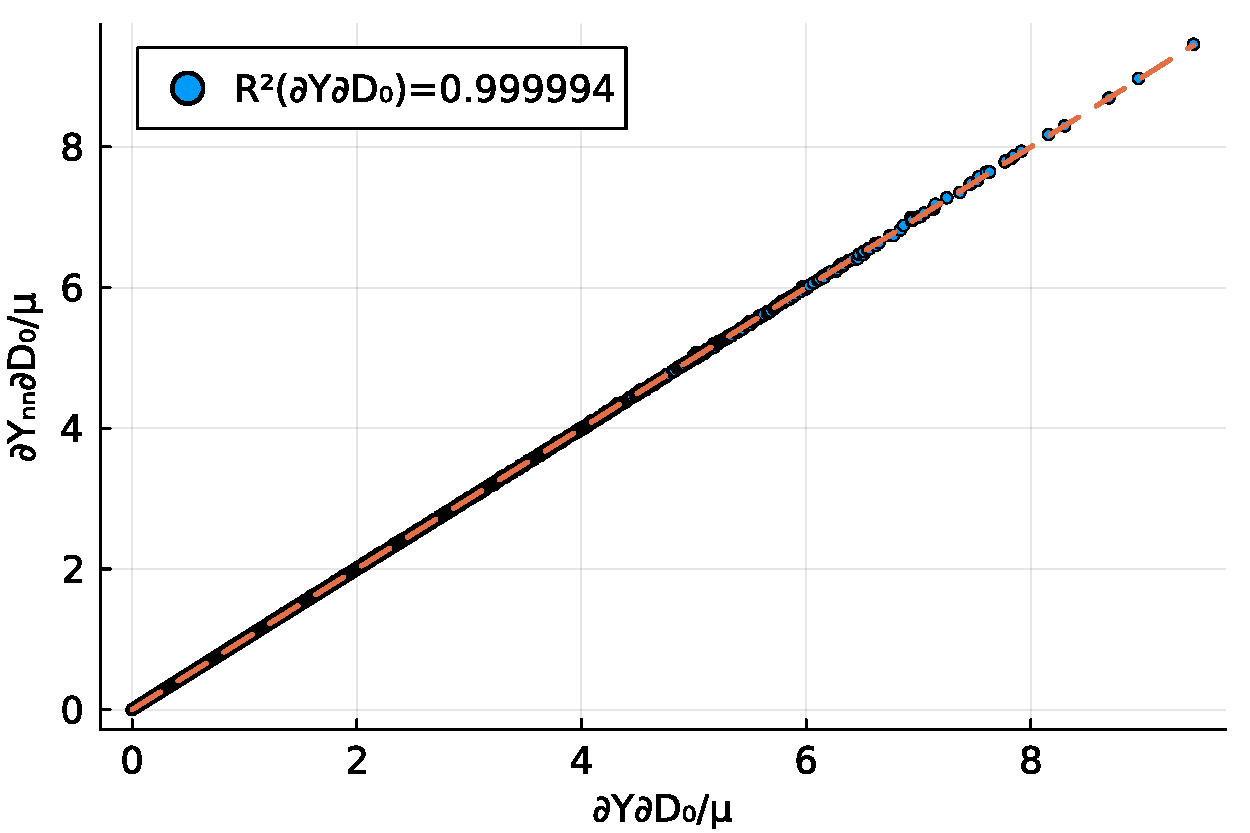
\includegraphics[width=0.33\textwidth]{Figures/PotentialStudy/Upsilon_E0_CorrelationTest} &
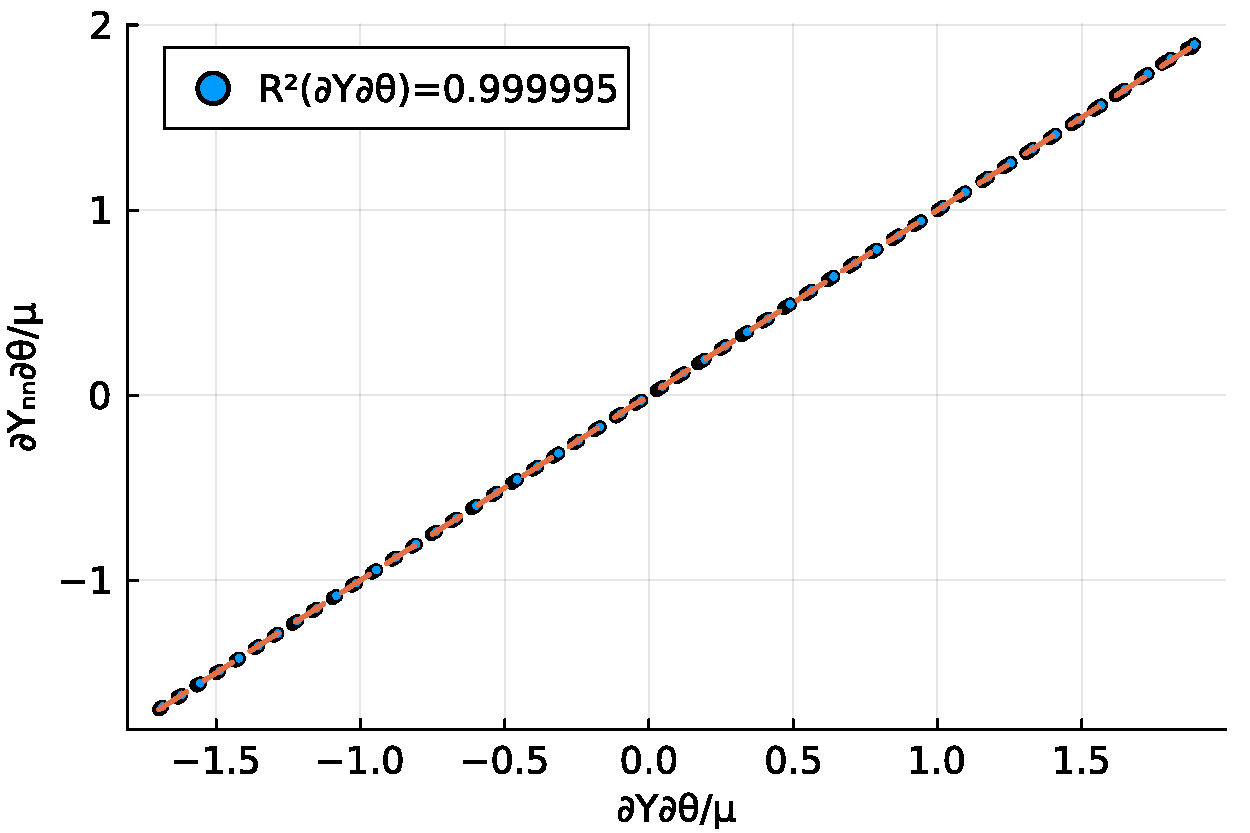
\includegraphics[width=0.33\textwidth]{Figures/PotentialStudy/Upsilon_theta_CorrelationTest} \\		%	
		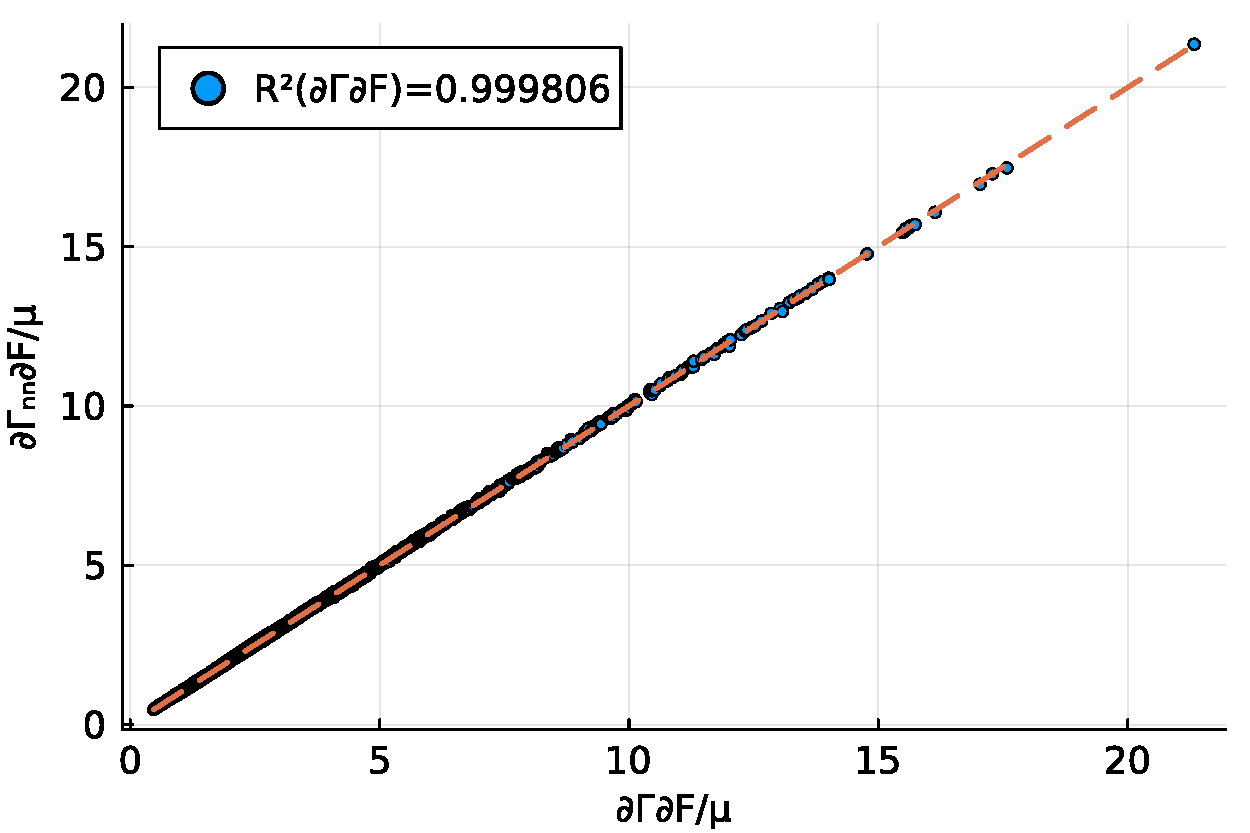
\includegraphics[width=0.33\textwidth]{Figures/PotentialStudy/Gamma_P_CorrelationTest} &
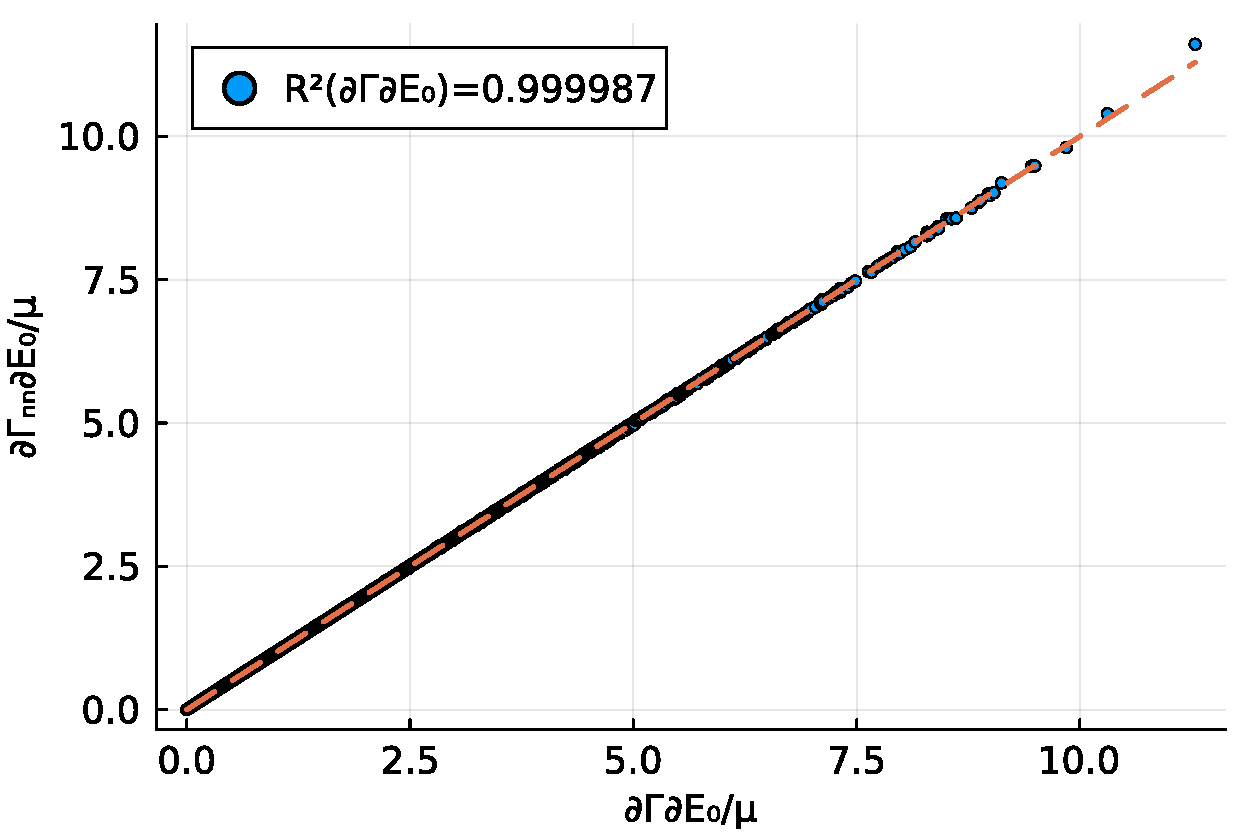
\includegraphics[width=0.33\textwidth]{Figures/PotentialStudy/Gamma_E0_CorrelationTest} &
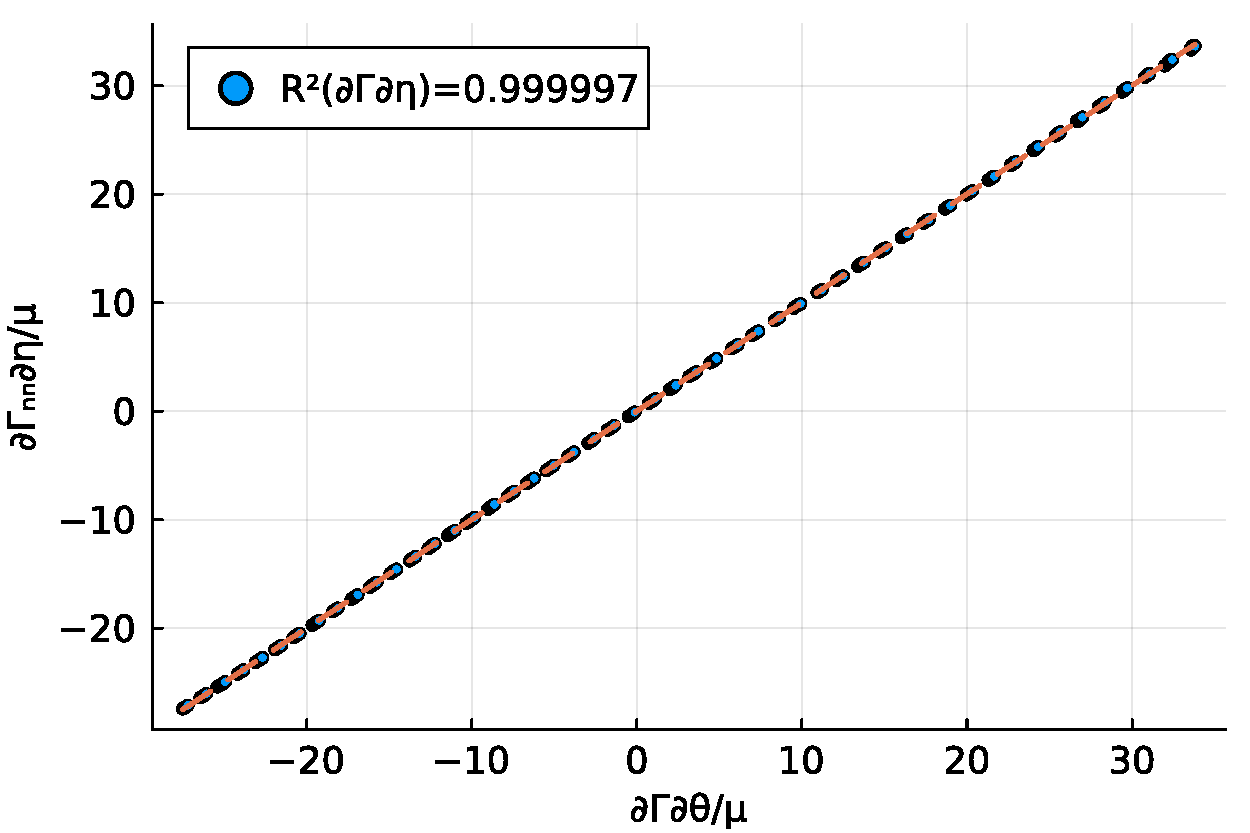
\includegraphics[width=0.33\textwidth]{Figures/PotentialStudy/Gamma_theta_CorrelationTest} \\		

	\end{tabular}
	%
	%		\includegraphics[width=0.4\textwidth]{pictures_paper/inkscape_pictures/template_example_3.pdf}
	\caption{\textbf{Calibration Strategy 1}. Correlation of prediction , $\{\partial_{\vect{F}}\Psi_{nn},\partial_{\vect{E}_0}\Psi_{nn},\partial_{\theta}\Psi_{nn}\}$, $\{\partial_{\vect{F}}e_{nn},\partial_{\vect{D}_0}d_{nn},\partial_{\eta}e_{nn}\}$, $\{\partial_{\vect{F}}\Upsilon_{nn},\partial_{\vect{D}_0}\Upsilon_{nn},\partial_{\theta}\Upsilon_{nn}\}$ and $\{\partial_{\vect{F}}\Gamma_{nn},\partial_{\vect{E}_0}\Gamma_{nn},\partial_{\eta}\Gamma_{nn}\}$ and their testing data counterparts. In all cases we have considered an architecture of $4$ layers and $8$ neurons per layer.}
	\label{fig:strategy 1--the potentials}
\end{figure}

\clearpage


\subsubsection{Polyconvex calibration}\label{sec:polyconvexity}

STUDY OF POLYCONVEXITY FOR POTENTIAL e

\begin{figure}[hbtp]
	\centering
	\begin{tabular}{ccc}
		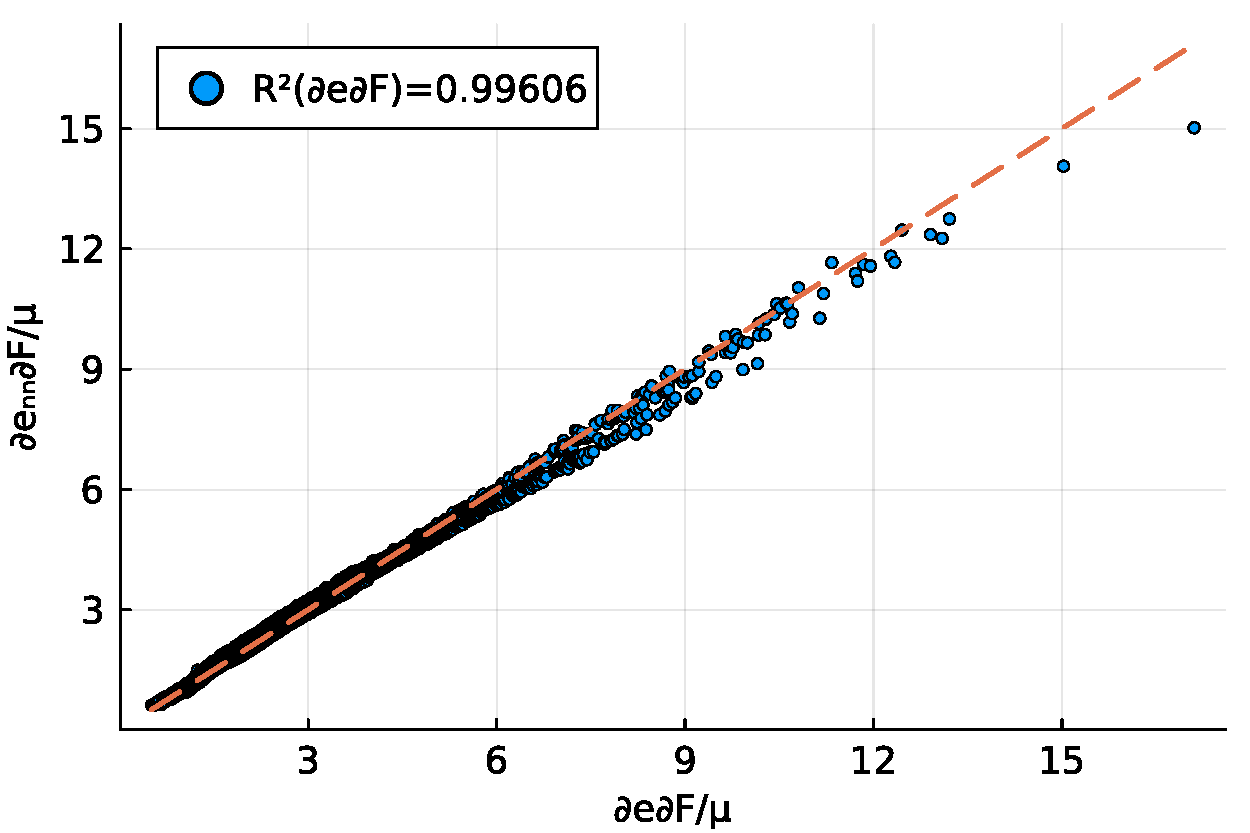
\includegraphics[width=0.33\textwidth]{Figures/PotentialStudy/e_pol_P_CorrelationTest} &
		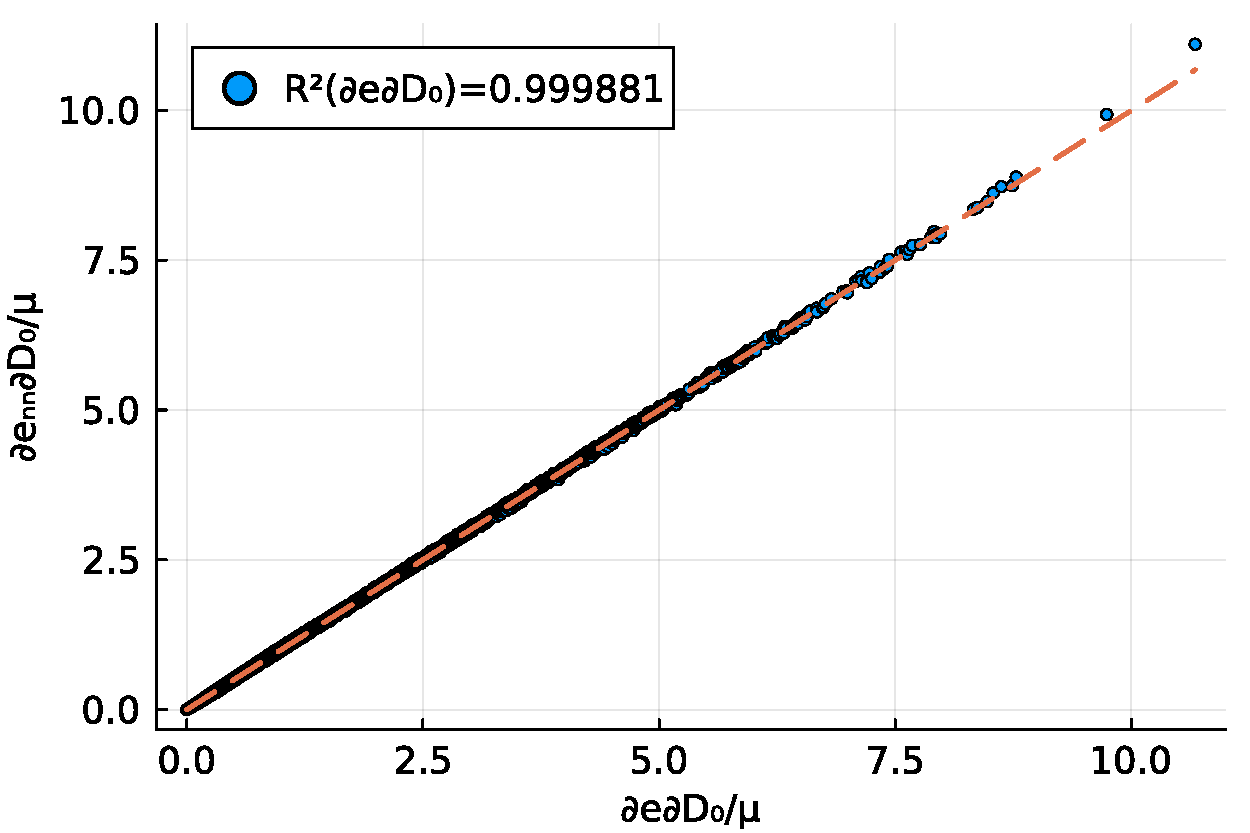
\includegraphics[width=0.33\textwidth]{Figures/PotentialStudy/e_pol_E0_CorrelationTest} &
		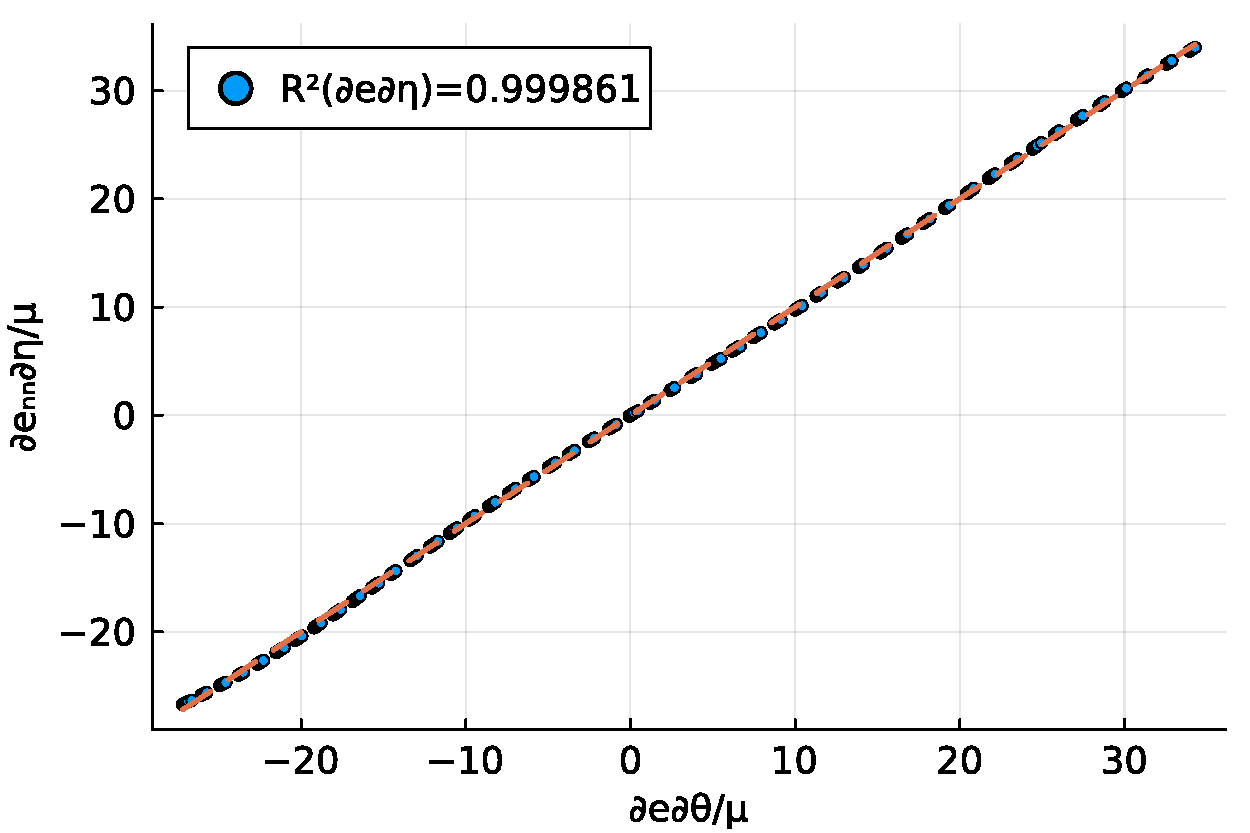
\includegraphics[width=0.33\textwidth]{Figures/PotentialStudy/e_pol_theta_CorrelationTest} \\

	\end{tabular}
	%
	%		\includegraphics[width=0.4\textwidth]{pictures_paper/inkscape_pictures/template_example_3.pdf}
	\caption{\textbf{Calibration Strategy 1}.}
	\label{fig:example 1 energy balance}
\end{figure}


\subsubsection{Generalization to unseen experiments}





\clearpage


\subsection{Calibration strategy 2: $\theta$-based potentials}


\subsubsection{Neural network architecture's influence: $\Psi_{nn}$ neural network-based ground truth models}


\begin{table}[hbtp!]
	\centering
	\begin{tabular}{c c c c c c c c c c c c}
		\toprule
		\rowcolor{gray!30}	\small{} & $n_L+1$ & 1 &  2& 3& 4& 5& 1& 2& 3& 4 & 5\\
		\midrule 
		\rowcolor{gray!30}	\small{} & $n_n$ & 8 & 8& 8& 8 &8 &16& 16& 16& 16 &  16\\
		\midrule
		\multirow{3}{*}{\rotatebox{90}{\textcolor{red}{\textbf{MR}}/\textcolor{blue}{\textbf{ID}}}}  &$R^2(\partial_{\vect{F}}\Psi)$ & 1 & 1& 1 & 1 & 1& 1& 1& 1& 1 & 1\\
		&$R^2(\partial_{\vect{F}}\Psi)$ & 1 & 1& 1 & 1 & 1& 1& 1& 1& 1 & 1\\
		&$R^2(\partial_{\vect{F}}\Psi)$ & 1 & 1& 1 & 1 & 1& 1& 1& 1& 1 & 1\\	
		\midrule
		\multirow{3}{*}{\rotatebox{90}{QMR/ID}} &$R^2(\partial_{\vect{F}}\Psi)$ & 1 & 1& 1 & 1 & 1& 1& 1& 1& 1 &  1\\
		&$R^2(\partial_{\vect{F}}\Psi)$ & 1 & 1& 1 & 1 & 1& 1& 1& 1& 1 &  1\\
		&$R^2(\partial_{\vect{F}}\Psi)$ & 1 & 1& 1 & 1 & 1& 1& 1& 1& 1 & 1\\	
		\midrule
		\multirow{3}{*}{\rotatebox{90}{Y/ID}} &$R^2(\partial_{\vect{F}}\Psi)$ & 1 & 1& 1 & 1 & 1& 1& 1& 1& 1 &  1\\
		&$R^2(\partial_{\vect{F}}\Psi)$ & 1 & 1& 1 & 1 & 1& 1& 1& 1& 1 &  1\\
		&$R^2(\partial_{\vect{F}}\Psi)$ & 1 & 1& 1 & 1 & 1& 1& 1& 1& 1 & 1\\	
		\midrule
		\multirow{3}{*}{\rotatebox{90}{G/ID}} &$R^2(\partial_{\vect{F}}\Psi)$ & 1 & 1& 1 & 1 & 1& 1& 1& 1& 1 &  1\\
		&$R^2(\partial_{\vect{F}}\Psi)$ & 1 & 1& 1 & 1 & 1& 1& 1& 1& 1 &  1\\
		&$R^2(\partial_{\vect{F}}\Psi)$ & 1 & 1& 1 & 1 & 1& 1& 1& 1& 1 & 1\\	
		\midrule
		\multirow{3}{*}{\rotatebox{90}{TI/ID}} &$R^2(\partial_{\vect{F}}\Psi)$ & 1 & 1& 1 & 1 & 1& 1& 1& 1& 1 &  1\\
		&$R^2(\partial_{\vect{F}}\Psi)$ & 1 & 1& 1 & 1 & 1& 1& 1& 1& 1 &  1\\
		&$R^2(\partial_{\vect{F}}\Psi)$ & 1 & 1& 1 & 1 & 1& 1& 1& 1& 1 & 1\\	
		\midrule
		\multirow{3}{*}{\rotatebox{90}{MR/ES}} &$R^2(\partial_{\vect{F}}\Psi)$ & 1 & 1& 1 & 1 & 1& 1& 1& 1& 1 &  1\\
		&$R^2(\partial_{\vect{F}}\Psi)$ & 1 & 1& 1 & 1 & 1& 1& 1& 1& 1 &  1\\
		&$R^2(\partial_{\vect{F}}\Psi)$ & 1 & 1& 1 & 1 & 1& 1& 1& 1& 1 & 1\\	
		\midrule
	\end{tabular}
	\caption{}
	\label{table: results calibration strategy 1}
\end{table}


\clearpage



\begin{figure}[hbtp!]
	\centering
	\begin{tabular}{cccc}
		\rotatebox{90}{\,\,\,\,\,\,\,\,\,\,\textcolor{red}{\textbf{MR}}/\textcolor{blue}{\textbf{ID}}}  &		\includegraphics[width=0.33\textwidth]{Figures/ModelsStudy/_MooneyRivlin_ID_E0_P_CorrelationTest} &
		\includegraphics[width=0.33\textwidth]{Figures/ModelsStudy/_MooneyRivlin_ID_E0_E0_CorrelationTest} &
		\includegraphics[width=0.33\textwidth]{Figures/ModelsStudy/_MooneyRivlin_ID_E0_theta_CorrelationTest} \\
		%
		\rotatebox{90}{\,\,\,\,\,\,\,\,\,\,\textcolor{red}{\textbf{QMR}}/\textcolor{blue}{\textbf{ID}}} &	\includegraphics[width=0.33\textwidth]{Figures/ModelsStudy/_QuadraticMooneyRivlin_ID_E0_P_CorrelationTest} &
		\includegraphics[width=0.33\textwidth]{Figures/ModelsStudy/_QuadraticMooneyRivlin_ID_E0_E0_CorrelationTest} &
		\includegraphics[width=0.33\textwidth]{Figures/ModelsStudy/_QuadraticMooneyRivlin_ID_E0_theta_CorrelationTest} \\
		%
		%
		\rotatebox{90}{\,\,\,\,\,\,\,\,\,\,\textcolor{red}{\textbf{Y}}/\textcolor{blue}{\textbf{ID}}}  &		\includegraphics[width=0.33\textwidth]{Figures/ModelsStudy/_Yeoh_ID_E0_P_CorrelationTest} &
		\includegraphics[width=0.33\textwidth]{Figures/ModelsStudy/_Yeoh_ID_E0_E0_CorrelationTest} &
		\includegraphics[width=0.33\textwidth]{Figures/ModelsStudy/_Yeoh_ID_E0_theta_CorrelationTest} \\
		%
		%
		\rotatebox{90}{\,\,\,\,\,\,\,\,\,\,\textcolor{red}{\textbf{G}}/\textcolor{blue}{\textbf{ID}}}  &		\includegraphics[width=0.33\textwidth]{Figures/ModelsStudy/_Gent_ID_E0_P_CorrelationTest} &
		\includegraphics[width=0.33\textwidth]{Figures/ModelsStudy/_Gent_ID_E0_E0_CorrelationTest} &
		\includegraphics[width=0.33\textwidth]{Figures/ModelsStudy/_Gent_ID_E0_theta_CorrelationTest} \\
		%
		%
		\rotatebox{90}{\,\,\,\,\,\,\,\,\,\,\textcolor{red}{\textbf{TI}}/\textcolor{blue}{\textbf{ID}}}  &		\includegraphics[width=0.33\textwidth]{Figures/ModelsStudy/_TI_ID_E0_P_CorrelationTest} &
		\includegraphics[width=0.33\textwidth]{Figures/ModelsStudy/_TI_ID_E0_E0_CorrelationTest} &
		\includegraphics[width=0.33\textwidth]{Figures/ModelsStudy/_TI_ID_E0_theta_CorrelationTest} \\
		%
		%
		\rotatebox{90}{\,\,\,\,\,\,\,\,\,\,\textcolor{red}{\textbf{MR}}/\textcolor{blue}{\textbf{ES}}}  &	\includegraphics[width=0.33\textwidth]{Figures/ModelsStudy/_MooneyRivlin_ElectricSaturation_P_CorrelationTest} &
		\includegraphics[width=0.33\textwidth]{Figures/ModelsStudy/_MooneyRivlin_ElectricSaturation_E0_CorrelationTest} &
		\includegraphics[width=0.33\textwidth]{Figures/ModelsStudy/_MooneyRivlin_ElectricSaturation_theta_CorrelationTest} \\
		%
		%
	\end{tabular}
	%
	%		\includegraphics[width=0.4\textwidth]{pictures_paper/inkscape_pictures/template_example_3.pdf}
	\caption{}
	\label{fig:example 1 energy balance}
\end{figure}



\clearpage

\subsubsection{Generalization results for $\Upsilon(\vect{F},\vect{D}_0,\theta)$}



\begin{figure}[hbtp]
	\centering
	\begin{tabular}{ccc}
		\includegraphics[width=0.33\textwidth]{Figures/PotentialStudy/Psi_P_CorrelationTest} &
		\includegraphics[width=0.33\textwidth]{Figures/PotentialStudy/Psi_E0_CorrelationTest} &
		\includegraphics[width=0.33\textwidth]{Figures/PotentialStudy/Psi_theta_CorrelationTest} \\
		%
		\includegraphics[width=0.33\textwidth]{Figures/PotentialStudy/e_P_CorrelationTest} &
		\includegraphics[width=0.33\textwidth]{Figures/PotentialStudy/e_E0_CorrelationTest} &
		\includegraphics[width=0.33\textwidth]{Figures/PotentialStudy/e_theta_CorrelationTest} \\		%	
		%	
		\includegraphics[width=0.33\textwidth]{Figures/PotentialStudy/Upsilon_P_CorrelationTest} &
		\includegraphics[width=0.33\textwidth]{Figures/PotentialStudy/Upsilon_E0_CorrelationTest} &
		\includegraphics[width=0.33\textwidth]{Figures/PotentialStudy/Upsilon_theta_CorrelationTest} \\		%	
		\includegraphics[width=0.33\textwidth]{Figures/PotentialStudy/Gamma_P_CorrelationTest} &
		\includegraphics[width=0.33\textwidth]{Figures/PotentialStudy/Gamma_E0_CorrelationTest} &
		\includegraphics[width=0.33\textwidth]{Figures/PotentialStudy/Gamma_theta_CorrelationTest} \\		
		
	\end{tabular}
	%
	%		\includegraphics[width=0.4\textwidth]{pictures_paper/inkscape_pictures/template_example_3.pdf}
	\caption{Numerical example 1. Evolution of: (a) angular momentum $\vect{J}$, (b) linear momentum $\vect{L}$, (c) global entropy $\tilde{\eta}=\int_{\mathcal{B}_0}\eta\,dV$, (d) Hamiltonian $\mathcal{H}$  in \eqref{eqn:Hamiltonian}, (e) increment of Hamiltonian $\Delta\mathcal{H}$ for both the Mid-Point and the new EM time integrator.  Finally, (f), zoomed detail of the increment of the Hamiltonian  $\Delta\mathcal{H}$ for the new EM time integrator. Results obtained for \textbf{Mesh2} with $\alpha_{CFL}=2.2955$ ($\Delta t=0.2$ s).}
	\label{fig:example 1 energy balance}
\end{figure}


\subsection{Calibration strategy 2: $\eta$-based potentials}


\subsubsection{Neural network architecture's influence: $e_{nn}$ neural network-based ground truth models}


\begin{table}[hbtp!]
	\centering
	\begin{tabular}{c c c c c c c c c c c c}
		\toprule
		\rowcolor{gray!30}	\small{} & $n_L+1$ & 1 &  2& 3& 4& 5& 1& 2& 3& 4 & 5\\
		\midrule 
		\rowcolor{gray!30}	\small{} & $n_n$ & 8 & 8& 8& 8 &8 &16& 16& 16& 16 &  16\\
		\midrule
		\multirow{3}{*}{\rotatebox{90}{\textcolor{red}{\textbf{MR}}/\textcolor{blue}{\textbf{ID}}}}  &$R^2(\partial_{\vect{F}}\Psi)$ & 1 & 1& 1 & 1 & 1& 1& 1& 1& 1 & 1\\
		&$R^2(\partial_{\vect{F}}\Psi)$ & 1 & 1& 1 & 1 & 1& 1& 1& 1& 1 & 1\\
		&$R^2(\partial_{\vect{F}}\Psi)$ & 1 & 1& 1 & 1 & 1& 1& 1& 1& 1 & 1\\	
		\midrule
		\multirow{3}{*}{\rotatebox{90}{\textcolor{red}{\textbf{QMR}}/\textcolor{blue}{\textbf{ID}}}} &$R^2(\partial_{\vect{F}}\Psi)$ & 1 & 1& 1 & 1 & 1& 1& 1& 1& 1 &  1\\
		&$R^2(\partial_{\vect{F}}\Psi)$ & 1 & 1& 1 & 1 & 1& 1& 1& 1& 1 &  1\\
		&$R^2(\partial_{\vect{F}}\Psi)$ & 1 & 1& 1 & 1 & 1& 1& 1& 1& 1 & 1\\	
		\\
		\midrule
		\multirow{3}{*}{\rotatebox{90}{\textcolor{red}{\textbf{Y}}/\textcolor{blue}{\textbf{ID}}}} &$R^2(\partial_{\vect{F}}\Psi)$ & 1 & 1& 1 & 1 & 1& 1& 1& 1& 1 &  1\\
		&$R^2(\partial_{\vect{F}}\Psi)$ & 1 & 1& 1 & 1 & 1& 1& 1& 1& 1 &  1\\
		&$R^2(\partial_{\vect{F}}\Psi)$ & 1 & 1& 1 & 1 & 1& 1& 1& 1& 1 & 1\\	
		\midrule
		\multirow{3}{*}{\rotatebox{90}{G/ID}} &$R^2(\partial_{\vect{F}}\Psi)$ & 1 & 1& 1 & 1 & 1& 1& 1& 1& 1 &  1\\
		&$R^2(\partial_{\vect{F}}\Psi)$ & 1 & 1& 1 & 1 & 1& 1& 1& 1& 1 &  1\\
		&$R^2(\partial_{\vect{F}}\Psi)$ & 1 & 1& 1 & 1 & 1& 1& 1& 1& 1 & 1\\	
		\midrule
		\multirow{3}{*}{\rotatebox{90}{TI/ID}} &$R^2(\partial_{\vect{F}}\Psi)$ & 1 & 1& 1 & 1 & 1& 1& 1& 1& 1 &  1\\
		&$R^2(\partial_{\vect{F}}\Psi)$ & 1 & 1& 1 & 1 & 1& 1& 1& 1& 1 &  1\\
		&$R^2(\partial_{\vect{F}}\Psi)$ & 1 & 1& 1 & 1 & 1& 1& 1& 1& 1 & 1\\	
		\midrule
		\multirow{3}{*}{\rotatebox{90}{MR/ES}} &$R^2(\partial_{\vect{F}}\Psi)$ & 1 & 1& 1 & 1 & 1& 1& 1& 1& 1 &  1\\
		&$R^2(\partial_{\vect{F}}\Psi)$ & 1 & 1& 1 & 1 & 1& 1& 1& 1& 1 &  1\\
		&$R^2(\partial_{\vect{F}}\Psi)$ & 1 & 1& 1 & 1 & 1& 1& 1& 1& 1 & 1\\	
		\midrule
	\end{tabular}
	\caption{}
	\label{table: results calibration strategy 1}
\end{table}


\clearpage



\begin{figure}[hbtp!]
	\centering
	\begin{tabular}{cccc}
		\rotatebox{90}{\,\,\,\,\,\,\,\,\,\,\textcolor{red}{\textbf{MR}}/\textcolor{blue}{\textbf{ID}}}  &		\includegraphics[width=0.33\textwidth]{Figures/ModelsStudy/_MooneyRivlin_ID_E0_P_CorrelationTest} &
		\includegraphics[width=0.33\textwidth]{Figures/ModelsStudy/_MooneyRivlin_ID_E0_E0_CorrelationTest} &
		\includegraphics[width=0.33\textwidth]{Figures/ModelsStudy/_MooneyRivlin_ID_E0_theta_CorrelationTest} %\\
		%
%		\rotatebox{90}{\,\,\,\,\,\,\,\,\,\,\textcolor{red}{\textbf{QMR}}/\textcolor{blue}{\textbf{ID}}} &	\includegraphics[width=0.33\textwidth]{Figures/ModelsStudy/_QuadraticMooneyRivlin_ID_E0_P_CorrelationTest} &
%		\includegraphics[width=0.33\textwidth]{Figures/ModelsStudy/_QuadraticMooneyRivlin_ID_E0_E0_CorrelationTest} &
%		\includegraphics[width=0.33\textwidth]{Figures/ModelsStudy/_QuadraticMooneyRivlin_ID_E0_theta_CorrelationTest} \\
		%
		%
%		\rotatebox{90}{\,\,\,\,\,\,\,\,\,\,\textcolor{red}{\textbf{Y}}/\textcolor{blue}{\textbf{ID}}}  &		\includegraphics[width=0.33\textwidth]{Figures/ModelsStudy/_Yeoh_ID_E0_P_CorrelationTest} &
%		\includegraphics[width=0.33\textwidth]{Figures/ModelsStudy/_Yeoh_ID_E0_E0_CorrelationTest} &
%		\includegraphics[width=0.33\textwidth]{Figures/ModelsStudy/_Yeoh_ID_E0_theta_CorrelationTest} \\
		%
		%
%		\rotatebox{90}{\,\,\,\,\,\,\,\,\,\,\textcolor{red}{\textbf{G}}/\textcolor{blue}{\textbf{ID}}}  &		\includegraphics[width=0.33\textwidth]{Figures/ModelsStudy/_Gent_ID_E0_P_CorrelationTest} &
%		\includegraphics[width=0.33\textwidth]{Figures/ModelsStudy/_Gent_ID_E0_E0_CorrelationTest} &
%		\includegraphics[width=0.33\textwidth]{Figures/ModelsStudy/_Gent_ID_E0_theta_CorrelationTest} \\
%		%
%		%
%		\rotatebox{90}{\,\,\,\,\,\,\,\,\,\,\textcolor{red}{\textbf{TI}}/\textcolor{blue}{\textbf{ID}}}  &		\includegraphics[width=0.33\textwidth]{Figures/ModelsStudy/_TI_ID_E0_P_CorrelationTest} &
%		\includegraphics[width=0.33\textwidth]{Figures/ModelsStudy/_TI_ID_E0_E0_CorrelationTest} &
%		\includegraphics[width=0.33\textwidth]{Figures/ModelsStudy/_TI_ID_E0_theta_CorrelationTest} \\
%		%
%		%
%		\rotatebox{90}{\,\,\,\,\,\,\,\,\,\,\textcolor{red}{\textbf{MR}}/\textcolor{blue}{\textbf{ES}}}  &	\includegraphics[width=0.33\textwidth]{Figures/ModelsStudy/_MooneyRivlin_ElectricSaturation_P_CorrelationTest} &
%		\includegraphics[width=0.33\textwidth]{Figures/ModelsStudy/_MooneyRivlin_ElectricSaturation_E0_CorrelationTest} &
%		\includegraphics[width=0.33\textwidth]{Figures/ModelsStudy/_MooneyRivlin_ElectricSaturation_theta_CorrelationTest} \\
		%
		%
	\end{tabular}
	%
	%		\includegraphics[width=0.4\textwidth]{pictures_paper/inkscape_pictures/template_example_3.pdf}
	\caption{}
	\label{fig:example 1 energy balance}
\end{figure}







\clearpage

\subsection{Finite Element numerical experiments}

The objective of this section is to study the performance of the newly proposed EM time integration scheme presented in equation \eqref{eqn:weak forms for proposed time integrator} in a variety of challenging examples, {with the aim of comparing the long-term stability of the new time integrator against that of the classical midpoint rule.}



\subsubsection{Numerical Example 1}


The objectives of this example are:
%
\begin{itemize}

\item \textbf{O1} To carry out a thorough analysis of the stability and robustness of the proposed EM time integrator comparing it against of the mid-point rule time integrator  as a function of the Courant-Friedrich-Lewy number for the case of Finite Element $h$-refinement. 

\item \textbf{O2}   For a given level of spatial discretisation refinement and time step, to compare the thermodynamical consistency of the proposed time integrator to that of the mid-point time integrator.


\end{itemize}	

The geometry for the problem is displayed in Figure \ref{fig:LShape geometry}. The L-shaped solid is subjected to an external torque induced by a pair of forces $\vect{F}_1(t)$ and $\vect{F}_2(t)$ acting on two of the boundary faces (refer to Figure \ref{fig:LShape geometry}), defined as
%
\begin{equation}\label{eqn:Torque}
\vect{F}_2(t)=-\vect{F}_1(t);\qquad
\vect{F}_1(t)=\begin{bmatrix}
256/9\\512/9\\768/9
\end{bmatrix}f(t);\qquad f(t)=\left\{\begin{array}{ccc}
\begin{aligned}
t&&0\leq t<2.5\,\text{s} ,\\
5-t&&2.5\,\text{s}\leq t<5\,\text{s}\\
0  &&t\geq 5\,\text{s}. 
\end{aligned} 
\end{array}\right.
\end{equation}

In addition, initial distribution of temperature on the solid is
%
\begin{equation}
\left.\theta(\vect{X})\right\vert_{t=0}=\left\{\begin{array}{ccc}
\begin{aligned}
T_1&&Z=L_Z ,\\
T_2&&X=L_X\\
\theta_R  &&\text{elsewhere}. 
\end{aligned} 
\end{array}\right.;\qquad
T_1=300\,K; \qquad  T_2=250\,K.
\end{equation} 


\begin{figure}[hbtp]
	\centering
	\includegraphics[width=0.3\textwidth]{Figures/Example1/LShape.pdf}
	%
	%		\includegraphics[width=0.4\textwidth]{pictures_paper/inkscape_pictures/template_example_3.pdf}
	\caption{Numerical example 1. Geometry and general setting.}
	\label{fig:LShape geometry}
\end{figure}
%


In order to establish a quantitative comparison with the results provided in Reference \cite{Betsch2018Thermo}, we use in this example the  constitutive model considered therein. This can be expressed in terms of the following additive decomposition,
%
\begin{equation}\label{eqn:Betsch model}
\begin{aligned}
\widetilde{W}\left(\vect{C},\vect{G},C,\theta\right)& = \widetilde{W}_{m}\left(\vect{C},\vect{G},C\right) + \widetilde{W}_{\theta}\left(\theta\right) - 
{(\theta-\theta_R)\widetilde{\eta}_R\left(C\right)},
\end{aligned}
\end{equation}
%
where each of the contributions in \eqref{eqn:Betsch model} is defined as
%
\begin{equation}\label{eqn:Betsch model II}
\begin{aligned}
 \widetilde{W}_{m}\left(\vect{C},\vect{G},C\right)&= \frac{\mu_1}{2}\text{tr}\vect{C} + \frac{\mu_2}{2}\text{tr}\vect{G} - \left(\mu_1 + 2\mu_2\right)\ln C^{1/2} + \frac{\lambda}{2}\left(C^{1/2}-1\right)^2;\\
 %
 \widetilde{W}_{\theta}(\theta)&=c_v\left(\theta - \theta_R - \theta \ln\frac{\theta}{\theta_R}\right);\quad
 %
 \widetilde{\eta}_R(C) = -3\beta\left(a(C^{1/2}-1) - bC^{-1/2}\right).
\end{aligned}
\end{equation}

The thermal conductivity tensor is particularised for the case of isotropy, whereby it can be expressed in terms of the scalar conductivity field $k$, i.e. $\vect{k} = k\vect{I}$. The value of all the relevant material and geometrical parameters in this example can be found in Table \ref{table:LShape parameters}.

\begin{table}[htbp]
	\centering
	\caption{Numerical example 1. Geometrical parameters (see Figure \ref{fig:LShape geometry}) and material parameters (see \eqref{eqn:Betsch model II}).}
	%
	\label{table:LShape parameters}
	%
	\vspace{2mm}
	\begin{tabular}{l | c c c l|}
		%\hline
		\cellcolor{gray!15}&&&&\\
		\cellcolor{gray!15}\textbf{Geometrical parameters}  &  $L_X$ &  6  &  m  &		\\
		%
		\cellcolor{gray!15}  &  $L_Y$ & 3 & m &\\
		%
		\cellcolor{gray!15}	&  $L_Z$ & 10 & m &\\
		%
		\hline
		%
		\cellcolor{gray!15}&&&\\
		\cellcolor{gray!15}\textbf{Material parameters}  &  $\mu_1$ &  1646,7  &  Pa &
		\\
		%
		\cellcolor{gray!15}&  $\mu_2$ & 332,5 & Pa &\\ %
		\cellcolor{gray!15}&  $\lambda$ & 0 & Pa &\\
		\cellcolor{gray!15}&  $c_v$ & 100 & $\text{J}\text{K}^{-1}\text{m}^{-3}$& \textit{(Specific heat capacity)}\\
		\cellcolor{gray!15}&  $\theta_R$ & 293.15 & K& \textit{(Reference temperature)}\\
		\cellcolor{gray!15}&  $\beta$ & $2,233\times10^{-4}$ & K$^{-1}$&\\
		\cellcolor{gray!15}&  $a$ & $\mu_1+  2\mu_2$ & Pa&\\
		\cellcolor{gray!15}&  $b$ & 0 & Pa&\\
		\cellcolor{gray!15}&  $k$ & 10 & WK$^{-1}$m$^{-1}$& \textit{(Thermal conductivity)}\\	
		\cellcolor{gray!15}&  $\rho_0$ & 100 & kg/$\text{m}^3$& \textit{(Material density)}\\				
		%
		%\hline
	\end{tabular}
\end{table}


\begin{figure}[hbtp]
	\centering
	\includegraphics[width=0.85\textwidth]{Figures/Example1/Meshesv2.pdf}
	%
	%		\includegraphics[width=0.4\textwidth]{pictures_paper/inkscape_pictures/template_example_3.pdf}
	\caption{Numerical example 1. $h$-refinement used in the study. $Q_1$-$Q_1$ finite element discretisation for both spatial geometry $\vect{\phi}$ and temperature $\theta$. From left to right: \textbf{Mesh1} (with $\{672,224\}$ dofs for $\{\vect{\phi},\theta\}$); \textbf{Mesh2} (refinement of $\times 2$ in every direction with respect to \textbf{Mesh1}, yielding $\{3822,1274\}$ dofs for $\{\vect{\phi},\theta\}$); \textbf{Mesh3} (refinement of $\times 3$ in every direction with respect to \textbf{Mesh1}, yielding $\{12000,4000\}$ dofs for $\{\vect{\phi},\theta\}$); \textbf{Mesh4} (refinement of $\times 4$ in every direction with respect to \textbf{Mesh1}, yielding $\{25350,8450\}$ dofs for $\{\vect{\phi},\theta\}$).}
	\label{fig:LShape meshes}
\end{figure}
%

Four different levels of $h$-refinement will be considered in this example. These can be observed in Figure \ref{fig:LShape meshes}. A course, medium,  fine and ulta fine finite element meshes (denoted as \textbf{Mesh1}, \textbf{Mesh2}, \textbf{Mesh3} and \textbf{Mesh4}, respectively) have been considered. With regards to objective $\textbf{O1}$,  we recall that the Courant-Friedrichs-Lewy number (denoted hereby as $\alpha_{CFL}$) is defined as
%
\begin{equation}\label{eqn:CFL}
\alpha_{CFL}=c_p\frac{\Delta t}{h};\qquad c_p=\sqrt{\frac{\lambda_R + 2\mu_R}{\rho_0}},
\end{equation}
%
where $\Delta t$ denotes the time step used in the simulations and $h$ the characteristic size of the finite element mesh, and $c_p$ the longitudinal wave speed in the reference configuartion ($\vect{\nabla}_0\vect{\phi}=\vect{I},\,\theta=\theta_R$). For hexahedral meshes, we consider $h$ to be related to the volume of the element $e$ in the mesh  (i.e. $V_e$) and to the order of the Finite Element interpolation $q$ (i.e. $q=1$ for $Q_1$ elements, $q=2$ for $Q_2$ elements, etc.) as
%
\begin{equation}
h = \left(\frac{\min\limits_{e}V_{e}}{q^3}\right)^{1/3};\qquad 1\leq e \leq N, 
\end{equation}
%
where $N$ denotes the number of elements for the underlying discretisation. 
%In addition, in \eqref{eqn:CFL}, $\{\mu_R,\lambda_R\}$ represent the shear and bulk moduli of the material in the origin (see equation \eqref{eqn:reference mechanical properties}). 
Figure \ref{fig:CFL study}$_a$ shows the final time instant $T_{final}$ for which the proposed EM time integrator fails, that is, \Blue{the time step for which the convergence of the iterative Netwon-Raphson algorithm is not achieved \cite{Kuhl_Crisfield_1996,Kuhl_Crisfield_1999}}, for different values of the $\alpha_{CFL}$ number and for the four levels of $h$-refinement displayed in Figure \ref{fig:LShape meshes}. Clearly, for large values of the $\alpha_{CFL}$ number, the new EM time integrator becomes unstable at smaller values of $T_{final}$, as expected. 


Figure \ref{fig:CFL study}$_b$ sheds light with regards to the relative stability of the proposed EM time integrator with respect to that of the classical mid-point time integrator. Specifically, this figure shows the difference between the final time instant for which the proposed EM time integrator and the mid-point rule become unstable. This has been denoted in that figure as $\Delta T_{final}$. \Blue{Contrary to the EM time integrator, for the mid-point integrator, the lack of convergence of the Newton-Raphson is always preceded by an uncontrollable growth of the Hamiltonian over the previous time steps.} Positive values of $\Delta T_{final}$ imply that the proposed time integrator becomes unstable at later time instants, and viceversa. It is worth noticing that beyond $\alpha_{CFL}\geq 5-10$,  $\Delta T_{final}$ adopts negative values. This indicates that the size of the time step $\Delta t$ cannot be chosen arbitrarily large, expecting an improved robustness and stability of the EM time integrator with respect to the classical mid-point rule. In fact our numerical study suggests that $\Delta t$ must be chosen such that $\alpha_{CFL}\leq 5$ in order to guarantee a higher stability and robustness in the long term.



\begin{figure}[hbtp]
	\centering
	\begin{tabular}{cc}
	\includegraphics[width=0.5\textwidth]{Figures/Example1/Tfinalv4.eps} &
%	\includegraphics[width=0.5\textwidth]{Figures/Example1/Tfinalv4.eps}
\includegraphics[width=0.5\textwidth]{Figures/Example1/DTfinalv4.eps}
	\end{tabular}
	%
	%		\includegraphics[width=0.4\textwidth]{pictures_paper/inkscape_pictures/template_example_3.pdf}
	\caption{Numerical example 1. Left: final time instant ($T_{final}$) for which the EM time integrator becomes unstable. Rigth: Difference between the final time instant ($\Delta T_{final}$) at which the EM time integrator and the mid-point rule become unstable. Results shown for various values of $\alpha_{CFL}$ and for the discretisations in Figure \ref{fig:LShape meshes}.}
	\label{fig:CFL study}
\end{figure}


\begin{figure}[hbtp]
	\centering
	\begin{tabular}{cc}
		\includegraphics[width=0.5\textwidth]{Figures/Example1/EnergyBalancePlots/Jv2.eps} &
		\includegraphics[width=0.5\textwidth]{Figures/Example1/EnergyBalancePlots/LinearMomentumv2.eps}\\
		%
	\includegraphics[width=0.5\textwidth]{Figures/Example1/EnergyBalancePlots/EntropyFinalv2.eps} &
\includegraphics[width=0.5\textwidth]{Figures/Example1/EnergyBalancePlots/EnergyFinalv2.eps}\\
%
	\includegraphics[width=0.5\textwidth]{Figures/Example1/EnergyBalancePlots/DHFinalv2.eps} &
\includegraphics[width=0.5\textwidth]{Figures/Example1/EnergyBalancePlots/DHEMv2.eps}\\
%		
	\end{tabular}
	%
	%		\includegraphics[width=0.4\textwidth]{pictures_paper/inkscape_pictures/template_example_3.pdf}
	\caption{Numerical example 1. Evolution of: (a) angular momentum $\vect{J}$, (b) linear momentum $\vect{L}$, (c) global entropy $\tilde{\eta}=\int_{\mathcal{B}_0}\eta\,dV$, (d) Hamiltonian $\mathcal{H}$  in \eqref{eqn:Hamiltonian}, (e) increment of Hamiltonian $\Delta\mathcal{H}$ for both the Mid-Point and the new EM time integrator.  Finally, (f), zoomed detail of the increment of the Hamiltonian  $\Delta\mathcal{H}$ for the new EM time integrator. Results obtained for \textbf{Mesh2} with $\alpha_{CFL}=2.2955$ ($\Delta t=0.2$ s).}
	\label{fig:example 1 energy balance}
\end{figure}


With regards to objective \textbf{O2}, we use in this study the computational domain defined by \textbf{Mesh2} (see Figure \ref{fig:LShape meshes}) and a value of $\alpha_{CFL}$ of $\alpha_{CFL}=2.2955$. It can be seen that for both the new EM time integrator and the mid-point rule the angular momentum $\vect{J}$ remains constant beyond $t\geq 5\,\textbf{s}$, when the external applied pair of forces vanishes. In addition, the linear momentum $\vect{L}$ is zero for the entire simulation. Another interesting variable of interest is the global entropy ($\tilde{\eta}=\int_{\mathcal{B}_0}\eta\,dV$), which increases over time for the entire simulation for both time integrators. Furthermore, the Hamiltonian $\mathcal{H}$ is displayed. The zoomed detail perfectly shows the sudden increase in the Hamiltonian $\mathcal{H}$ prior to the instability when using the mid-point rule. The increase of the Hamiltonian $\Delta \mathcal{H}={\mathcal{H}_{n+1}-\mathcal{H}_n}$ (normalised with respect to the maximum historic value of $\mathcal{H}$ in absolute value) is also displayed. It can be seen that the new EM time integrator preserves $\mathcal{H}$ (beyond $t\geq 5\,\text{s}$) as it has been designed specifically with that purpose, whereas the mid-point rule does not. 

Finally, the temperature contour plot is displayed over time in Figure \ref{fig:example 1 temperature}. The results have been obtained by means of the new EM time integrator using a different mesh from the four depicted in Figure \ref{fig:LShape meshes}. This mesh has been generated refining by a factor of $\times 6$ in the three directions the computational domain defined by \textbf{Mesh1}.



%\begin{figure}[hbtp]
%	\centering
%	\begin{tabular}{ccc}
%		\includegraphics[width=0.26\textwidth]{Figures/Example1/Pressure/RainBowBright/PressureNoMeshTimeStep25v2} &
%		\includegraphics[width=0.24\textwidth]{Figures/Example1/Pressure/RainBowBright/PressureNoMeshTimeStep50v2}
%		\includegraphics[width=0.40\textwidth]{Figures/Example1/Pressure/RainBowBright/PressureNoMeshTimeStep80v2} 
%		\\
%		\includegraphics[width=0.35\textwidth]{Figures/Example1/Pressure/RainBowBright/PressureNoMeshTimeStep110v2} &
%		\includegraphics[width=0.26\textwidth]{Figures/Example1/Pressure/RainBowBright/PressureNoMeshTimeStep150v2}
%		\includegraphics[width=0.36\textwidth]{Figures/Example1/Pressure/RainBowBright/PressureNoMeshTimeStep190v2} 
%		\\
%		\includegraphics[width=0.36\textwidth]{Figures/Example1/Pressure/RainBowBright/PressureNoMeshTimeStep210v2} &
%\includegraphics[width=0.24\textwidth]{Figures/Example1/Pressure/RainBowBright/PressureNoMeshTimeStep250v2}
%\includegraphics[width=0.24\textwidth]{Figures/Example1/Pressure/RainBowBright/PressureNoMeshTimeStep330v2} 		\\
%%
%		\includegraphics[width=0.25\textwidth]{Figures/Example1/Pressure/RainBowBright/PressureNoMeshTimeStep350v2} &
%\includegraphics[width=0.36\textwidth]{Figures/Example1/Pressure/RainBowBright/PressureNoMeshTimeStep400v2}
%\includegraphics[width=0.25\textwidth]{Figures/Example1/Pressure/RainBowBright/PressureNoMeshTimeStep430v2} 		
%	\end{tabular}
%	%
%	%		\includegraphics[width=0.4\textwidth]{pictures_paper/inkscape_pictures/template_example_3.pdf}
%	\caption{Numerical example 1. XX.}
%	\label{fig:example 1 pressure}
%\end{figure}
%%



%\begin{figure}[hbtp]
%	\centering
%	\begin{tabular}{ccc}
%		\includegraphics[width=0.21\textwidth]{Figures/Example1/Pressure/JetColor/PressureNoMeshJetTimeStep25v2} &
%		\includegraphics[width=0.17\textwidth]{Figures/Example1/Pressure/JetColor/PressureNoMeshJetTimeStep50v2}
%		\includegraphics[width=0.35\textwidth]{Figures/Example1/Pressure/JetColor/PressureNoMeshJetTimeStep80v2} 
%		\\
%		\includegraphics[width=0.30\textwidth]{Figures/Example1/Pressure/JetColor/PressureNoMeshJetTimeStep110v2} &
%		\includegraphics[width=0.21\textwidth]{Figures/Example1/Pressure/JetColor/PressureNoMeshJetTimeStep150v2}
%		\includegraphics[width=0.33\textwidth]{Figures/Example1/Pressure/JetColor/PressureNoMeshJetTimeStep190v2} 
%		\\
%		\includegraphics[width=0.29\textwidth]{Figures/Example1/Pressure/JetColor/PressureNoMeshJetTimeStep210v2} &
%		\includegraphics[width=0.19\textwidth]{Figures/Example1/Pressure/JetColor/PressureNoMeshJetTimeStep250v2}
%		\includegraphics[width=0.19\textwidth]{Figures/Example1/Pressure/JetColor/PressureNoMeshJetTimeStep330v2} 		\\
%		%
%		\includegraphics[width=0.20\textwidth]{Figures/Example1/Pressure/JetColor/PressureNoMeshJetTimeStep350v2} &
%		\includegraphics[width=0.31\textwidth]{Figures/Example1/Pressure/JetColor/PressureNoMeshJetTimeStep400v2}
%		\includegraphics[width=0.22\textwidth]{Figures/Example1/Pressure/JetColor/PressureNoMeshJetTimeStep430v2} 		
%	\end{tabular}
%%
%		\includegraphics[width=0.5\textwidth]{Figures/Example1/Pressure/JetColor/ColorBar} 		
%	%
%	%		\includegraphics[width=0.4\textwidth]{pictures_paper/inkscape_pictures/template_example_3.pdf}
%	\caption{Numerical example 1. XX.}
%	\label{fig:example 1 pressure}
%\end{figure}


%\begin{figure}[hbtp]
%	\centering
%	\begin{tabular}{ccc}
%		\includegraphics[width=0.21\textwidth]{Figures/Example1/Temperature/TimeStep25v2} &
%		\includegraphics[width=0.17\textwidth]{Figures/Example1/Temperature/TimeStep50v2}
%		\includegraphics[width=0.35\textwidth]{Figures/Example1/Temperature/TimeStep80v2} 
%		\\
%		\includegraphics[width=0.30\textwidth]{Figures/Example1/Temperature/TimeStep110v2} &
%		\includegraphics[width=0.21\textwidth]{Figures/Example1/Temperature/TimeStep150v2}
%		\includegraphics[width=0.33\textwidth]{Figures/Example1/Temperature/TimeStep190v2} 
%		\\
%		\includegraphics[width=0.29\textwidth]{Figures/Example1/Temperature/TimeStep210v2} &
%		\includegraphics[width=0.19\textwidth]{Figures/Example1/Temperature/TimeStep250v2}
%		\includegraphics[width=0.19\textwidth]{Figures/Example1/Temperature/TimeStep330v2} 		\\
%		%
%		\includegraphics[width=0.20\textwidth]{Figures/Example1/Temperature/TimeStep350v2} &
%		\includegraphics[width=0.31\textwidth]{Figures/Example1/Temperature/TimeStep400v2}
%		\includegraphics[width=0.22\textwidth]{Figures/Example1/Temperature/TimeStep430v2} 		
%	\end{tabular}
%	%
%		\includegraphics[width=0.5\textwidth]{Figures/Example1/Temperature/ColorBar} 			
%	%		\includegraphics[width=0.4\textwidth]{pictures_paper/inkscape_pictures/template_example_3.pdf}
%	\caption{Numerical example 1. XX.}
%	\label{fig:example 1 pressure}
%\end{figure}



\begin{figure}[hbtp]
	\centering
	\begin{tabular}{ccc}
		\includegraphics[width=0.12\textwidth]{Figures/Example1/Temperature/TS25v2} &
		\includegraphics[width=0.13\textwidth]{Figures/Example1/Temperature/TS50v2} &
		\includegraphics[width=0.27\textwidth]{Figures/Example1/Temperature/TS80v2} \\
		\includegraphics[width=0.23\textwidth]{Figures/Example1/Temperature/TS110v2} &
		\includegraphics[width=0.15\textwidth]{Figures/Example1/Temperature/TS150v2} &
		\includegraphics[width=0.26\textwidth]{Figures/Example1/Temperature/TS190v2} \\ 	
		\includegraphics[width=0.22\textwidth]{Figures/Example1/Temperature/TS210v2} &
		\includegraphics[width=0.12\textwidth]{Figures/Example1/Temperature/TS250v2}&
		%
		\includegraphics[width=0.12\textwidth]{Figures/Example1/Temperature/TS330v2}\\ 				
		%
		\includegraphics[width=0.16\textwidth]{Figures/Example1/Temperature/TS350v2} &
		\includegraphics[width=0.25\textwidth]{Figures/Example1/Temperature/TS400v2} &
		\includegraphics[width=0.13\textwidth]{Figures/Example1/Temperature/TS430v2} 		
	\end{tabular}
	%
	\includegraphics[width=0.5\textwidth]{Figures/Example1/Temperature/TSColorBarv2} 			
	%		\includegraphics[width=0.4\textwidth]{pictures_paper/inkscape_pictures/template_example_3.pdf}
	\vspace{-2mm}
	%
	\caption{Numerical example 1. Contour plot distribution of absolute temperature $T(K)$ for $t=\{2.5,5,8,11,15,19,21,25,33,35,40,43\}\,\text{s}$ (from left to right and top to bottom). $Q_1$-$Q_1$ discretisation for both spatial geometry $\vect{\phi}$ and temperature $\theta$. Number of dofs in the mesh: $\{85557,28519\}$ for $\{\vect{\phi},\theta\}$. Results obtained by means of the new EM time integrator for $\alpha_{CFL}=3.44$ ($\Delta t = 0.1\,\text{s}$).}
	\label{fig:example 1 temperature}
\end{figure}




\newpage


\subsection{Numerical Example 2}

The objective of this example is

\begin{itemize}
	\item \textbf{O1}   Study the stability and robustness in a problem where the deformation is exclusively induced by thermal effects.
	
\end{itemize}	

The geometry for this example is displayed in Figure \ref{fig:Bending actuator geometry}. The object in Figure \ref{fig:Bending actuator geometry} is  subjected to a heat flux at the bottom surface (minimum coordinate $Z$),  characterised by the following mathematical expression
%
\begin{equation}\label{eqn:Heat Flux}
Q_{\theta}(t)=Q_{\text{max}}\sin{\frac{2\pi}{T}t};\qquad T=1\,\text{s};\qquad Q_{\text{max}}=3000\,\mathrm{{W/m^2}}.
\end{equation}


\begin{figure}[hbtp]
	\centering
	\includegraphics[width=0.9\textwidth]{Figures/Example3/TheActuatorAndMeshForStudy.eps}
	%	\begin{tabular}{cc}
	%	\includegraphics[width=0.7\textwidth]{Figures/Example3/TheActuator.eps}&
	%    \includegraphics[width=0.3\textwidth]{Figures/Example3/MeshForStudy}
	%	\end{tabular}
	%
	%		\includegraphics[width=0.4\textwidth]{pictures_paper/inkscape_pictures/template_example_3.pdf}
	\caption{Numerical example 2. Left: geometry and general setting for the bi-material thermo-mechanical actuator. Right: computational domain considered for the analysis of $\textbf{O1}$, based on a  $Q_2$ discretisation for $\{\vect{x},T\}$, ($\{1215,405\}$ dofs). Every $Q_2$ finite element has been divided into $2\times 2\times 2$ elements for visualisation purposes.}
	\label{fig:Bending actuator geometry}
\end{figure}
%

The constitutive model used in this example is that presented in Section \ref{sec:constitutive models} through equations \eqref{eqn:additive decomposition}, \eqref{eqn:MRv2}, \eqref{eqn:thermal contribution} and \eqref{eqn:coupled contribution}. The value of the material parameters in that model can be found in {Table \ref{table:Bending actuator parameters}}.
%\begin{equation}
%\begin{aligend}
%\vect{v} = 20\sqrt{\frac{\pi}{2}}
%\end{aligned}
%\end{equation}

\begin{table}[htbp]
	\centering
	\caption{Numerical example 2. Geometrical parameters (see Figure \Blue{\ref{fig:Bending actuator geometry}}) and material parameters (see \eqref{eqn:Betsch model II}).}
	%
	\label{table:Bending actuator parameters}
	%
	\vspace{2mm}
	\begin{tabular}{l | c c c l|}
		%\hline
		\cellcolor{gray!15}&&&&\\
		\cellcolor{gray!15}\textbf{Geometrical parameters}  &  $L$ &  0,12  &  m  &		\\
		%
		\cellcolor{gray!15} &  $b$ & 0,06 & m &\\
		\cellcolor{gray!15} &  $H$ & 0,001 & m &\\		
		%
		\cellcolor{gray!15}&  $R$ & 0,01 & m &\\
		%
		\hline
		%
		\cellcolor{gray!15}&&&\\
		%%%%%%%%%%%
		%%%%%%%%%%%
		\cellcolor{gray!15}\textbf{Material parameters A} &   $\mu_1$ &  41.67  &  kPa &
		\\
		%
		\cellcolor{gray!15}&   $\mu^A_2$ & 0 & Pa &\\ %
		\cellcolor{gray!15}&  $\lambda^A$ & 27.78 & Pa &\\
		\cellcolor{gray!15}&  $c^A_v$ & 2000 & $\text{J}\text{K}^{-1}\text{m}^{-3}$& \textit{(Specific heat capacity)}\\
		\cellcolor{gray!15}&  $\theta^A_R$ & 293,15 & K& \textit{(Reference temperature)}\\
		\cellcolor{gray!15}&  $\Gamma^A_0$ & $0$ & &\\
		\cellcolor{gray!15}&  $q^A$ & 1 & &\\
		\cellcolor{gray!15}&  $k^A$ & 10 & WK$^{-1}$m$^{-1}$& \textit{(Thermal conductivity)}\\	
		\cellcolor{gray!15}&  $\rho^A_0$ & 1000 & kg/$\text{m}^3$& \textit{(Material density)}\\				
		%
		%
		%
		\hline
		\cellcolor{gray!15}&&&\\
		
		%%
		\cellcolor{gray!15}\textbf{Material parameters B} &   $\mu^B_1$ &  250  &  kPa &
		\\
		%
		\cellcolor{gray!15}&   $\mu^B_2$ & 0 & Pa &\\ %
		\cellcolor{gray!15}&  $\lambda^B$ & 166 & Pa &\\
		\cellcolor{gray!15}&  $c^B_v$ & 2000 & $\text{J}\text{K}^{-1}\text{m}^{-3}$& \textit{(Specific heat capacity)}\\
		\cellcolor{gray!15}&  $\theta^B_R$ & 293,15 & K& \textit{(Reference temperature)}\\
		\cellcolor{gray!15}&  $\Gamma^B_0$ & $0.01$ & &\\
		\cellcolor{gray!15}&  $q^B$ & 1 & &\\
		\cellcolor{gray!15}&  $k^B$ & 10 & WK$^{-1}$m$^{-1}$& \textit{(Thermal conductivity)}\\	
		\cellcolor{gray!15}&  $\rho^B_0$ & 1000 & kg/$\text{m}^3$& \textit{(Material density)}\\						
		%
		%\hline
	\end{tabular}
\end{table}


With regards to objective \textbf{O1}, we use in this study the computational domain defined in Figure \ref{fig:Bending actuator geometry} and several values of $\alpha_{CFL}$. From Figure \ref{fig:example 3 Stability analysis}$_{(a)}$-$_{(b)}$ it can be observed that the range of stability of the new EM time integrator is larger than that of the mid-point rule for approximately $\alpha_{CFL}\leq 10$ (close to zero and even negative values of $\Delta T_{final}$ are obtained in the range $\alpha_{CFL}\geq 10$). 
For a fixed value of $\alpha_{CFL}=5.6$ ($\Delta t =4\times 10^{-4}$ s), Figure \ref{fig:example 3 Stability analysis}$_{(c)}$ shows the evolution of the Hamiltonian in equation \eqref{eqn:Hamiltonian} for both the new EM time integrator and the mid-point rule. In this case, the non-vanishing heat flux $Q_{\theta}$ \eqref{eqn:Heat Flux} prevents the Hamiltonian from being preserved. Nonetheless, from equations \eqref{eqn:balance of energy final}, \eqref{eqn:Hamiltonian} and \eqref{conservation of energy discrete V}, it is clear that the quantity of interest defined as
%
\begin{equation}\label{eqn:tildeH}
\widetilde{\mathcal{H}}=\mathcal{H} - \Pi_{\text{ext}} - \mathcal{Q}_{\text{ext}} 
\end{equation}
%
must be preserved by the new EM time integrator. This in fact confirmed in Figure \ref{fig:example 3 Stability analysis}$_{(d)}$, where $\widetilde{\mathcal{H}}$ is perfectly preserved throughout the entire simulation by the new proposed time integrator. On the contrary, $\widetilde{\mathcal{H}}$ increases over time when using the mid-point time integrator until it finally becomes unstable. Finally, Figure \ref{fig:example 3 pressure 1}  shows the pressure contour plot over various snapshots computed by means of the new EM time integrator using the computational domain defined in Figure \ref{fig:example 3 Mesh}.





%\begin{figure}[hbtp]
%	\centering
%	\begin{tabular}{cc}
%		\includegraphics[width=0.5\textwidth]{Figures/Example1/EnergyBalancePlots/J.eps} &
%		\includegraphics[width=0.5\textwidth]{Figures/Example1/EnergyBalancePlots/LinearMomentum.eps}\\
%		%
%		\includegraphics[width=0.5\textwidth]{Figures/Example1/EnergyBalancePlots/EntropyFinal.eps} &
%		\includegraphics[width=0.5\textwidth]{Figures/Example1/EnergyBalancePlots/EnergyFinal.eps}\\
%		%
%		\includegraphics[width=0.5\textwidth]{Figures/Example1/EnergyBalancePlots/DHFinal.eps} &
%		\includegraphics[width=0.5\textwidth]{Figures/Example1/EnergyBalancePlots/DH_EM.eps}\\
%		%		
%	\end{tabular}
%	%
%	%		\includegraphics[width=0.4\textwidth]{pictures_paper/inkscape_pictures/template_example_3.pdf}
%	\caption{Numerical example 3. \Red{Evolution of: (a) angular momentum $\vect{J}$, (b) linear momentum $\vect{L}$, (c) global entropy $\tilde{\eta}=\int_{\mathcal{B}_0}\eta\,dV$, (d) Hamiltonian $\mathcal{H}$  in \eqref{eqn:Hamiltonian}, (e) increment of Hamiltonian $\Delta\mathcal{H}$ for both the Mid-Point and the new EM time integrator.  Finally, (f), zoomed detail of the increment of the Hamiltonian  $\Delta\mathcal{H}$ for the new EM time integrator. Results obtained for mesh in Figure \ref{fig:Bending actuator geometry} with $\alpha_{CFL}=5.6$ ($\Delta t=4\times 10^{-4}$ $(s)$).}}
%	\label{fig:CFL study bending actuator}
%\end{figure}


%\begin{figure}[hbtp]
%	\centering
%	\begin{tabular}{ccc}
%		\includegraphics[width=0.33\textwidth]{Figures/Example3/Pressure/TS73v2} &
%		\includegraphics[width=0.33\textwidth]{Figures/Example3/Pressure/TS422v2}
%		\includegraphics[width=0.32\textwidth]{Figures/Example3/Pressure/TS562v2} 
%		\\
%		\includegraphics[width=0.33\textwidth]{Figures/Example3/Pressure/TS585v2} &
%		\includegraphics[width=0.23\textwidth]{Figures/Example3/Pressure/TS878v2}
%		\includegraphics[width=0.23\textwidth]{Figures/Example3/Pressure/TS897v2} 
%		\\
%		\includegraphics[width=0.26\textwidth]{Figures/Example3/Pressure/TS1124v2} &
%		\includegraphics[width=0.23\textwidth]{Figures/Example3/Pressure/TS1353v2}
%		\includegraphics[width=0.23\textwidth]{Figures/Example3/Pressure/TS1527v2} 		\\
%		%
%		\includegraphics[width=0.28\textwidth]{Figures/Example3/Pressure/TS1729v2} &
%		\includegraphics[width=0.27\textwidth]{Figures/Example3/Pressure/TS1892v2}
%		\includegraphics[width=0.29\textwidth]{Figures/Example3/Pressure/TS2103v2} 		
%	\end{tabular}
%	%
%	\includegraphics[width=0.5\textwidth]{Figures/Example3/Pressure/ColorBarv2} 		
%	%
%	%		\includegraphics[width=0.4\textwidth]{pictures_paper/inkscape_pictures/template_example_3.pdf}
%	\caption{Numerical example 1. XX.}
%	\label{fig:example 2 pressure}
%\end{figure}
%
%%

%Figure \ref{fig:example 3 Displacement and Temperature evolution}
%displays the $Z$ and $Y$ components of the displacement in point $P$ (see Figure \ref{fig:Bending actuator geometry}) and Figures \ref{fig:example 3 pressure 1} and \ref{fig:example 3 pressure 2} show the pressure contour plot over various snapshots computed by means of the new EM time integrator using the computational domain defined in Figure \ref{fig:example 3 Mesh}.

%\begin{figure}[hbtp]
%	\centering
%	\begin{tabular}{cc}
%		\includegraphics[width=0.5\textwidth]{Figures/Example3/DisplacementEvolution.eps} &
%		\includegraphics[width=0.5\textwidth]{Figures/Example3/TemperatureEvolutionWithDetail.eps}
%		%		
%	\end{tabular}
%	%
%	%		\includegraphics[width=0.4\textwidth]{pictures_paper/inkscape_pictures/template_example_3.pdf}
%	\caption{Numerical example 3. Left: time evolution of $Y$ and $Z$ components of displacement of point $P$ (see Figure \ref{fig:Bending actuator geometry}); Right: time evolution of temperature at the same point. Results obtained with new EM time integrator and with $\alpha_{CFL}=5$ ($\Delta t=x \,(s)$). Computational domain in Figure \ref{fig:example 3 Mesh}.}
%	\label{fig:example 3 Displacement and Temperature evolution}
%\end{figure}




\begin{figure}[hbtp]
	\centering
	\begin{tabular}{cc}
		\includegraphics[width=0.5\textwidth]{Figures/Example3/EnergyBalance/TFinalv2.eps} &
		\includegraphics[width=0.5\textwidth]{Figures/Example3/EnergyBalance/DTv2.eps}\\(a)  &  (b)\\		
		\includegraphics[width=0.5\textwidth]{Figures/Example3/EnergyBalance/Energy.eps} &
		\includegraphics[width=0.5\textwidth]{Figures/Example3/EnergyBalance/DEnergy.eps}\\
		{{(c)}}& 		{{(d)}}
		%		
		%		
	\end{tabular}
	%
	%		\includegraphics[width=0.4\textwidth]{pictures_paper/inkscape_pictures/template_example_3.pdf}
	\caption{Numerical example 2. (a) Final time instant ($T_{final}$) for which the EM time integrator becomes unstable. (b) Difference between the final time instant ($\Delta T_{final}$) at which the EM time integrator and the mid-point rule become unstable. Results shown for various values of $\alpha_{CFL}=\{5.6,11.21,22.42\}\,(\Delta t=\{4,8,16\}\times 10^{-4}\,\text{s})$ and for the computational domain displayed. (c) Evolution of the Hamiltonian $\mathcal{H}$ \eqref{eqn:Hamiltonian} when using the mid-point rule and the new EM time integrator for $\alpha_{CFL}=5.6$. (d) Evolution of the quantity of interest $\widetilde{\mathcal{H}}$ in \eqref{eqn:tildeH} for both mid-point rule and the new EM time integrator for $\alpha_{CFL}=5.6$.}
	\label{fig:example 3 Stability analysis}
\end{figure}


\begin{figure}[hbtp]
	\centering
	\includegraphics[width=0.6\textwidth]{Figures/Example3/MeshAndDetail.eps}
	%
	%		\includegraphics[width=0.4\textwidth]{pictures_paper/inkscape_pictures/template_example_3.pdf}
	\caption{Numerical example 2. Computational domain discretised with $Q_2$ elements for both geometry $\vect{\phi}$ and temperature $\theta$. Discretisation of $\{164430,54810\}$ dofs for $\{\vect{\phi},\theta\}$. In the figure every $Q_2$ finite element has been divided into $2\times 2\times 2$ elements for visualisation purposes.}
	\label{fig:example 3 Mesh}
\end{figure}


%\begin{figure}[hbtp]
%	\centering
%	\begin{tabular}{cc}
%		\includegraphics[width=0.35\textwidth]{Figures/Example3/PressureNew/TS40Final} &
%		\includegraphics[width=0.35\textwidth]{Figures/Example3/PressureNew/TS60Final}
%		\\
%		\includegraphics[width=0.35\textwidth]{Figures/Example3/PressureNew/TS120Final} &
%		\includegraphics[width=0.35\textwidth]{Figures/Example3/PressureNew/TS160Final}
%		\\
%		\includegraphics[width=0.35\textwidth]{Figures/Example3/PressureNew/TS200Final} &
%		\includegraphics[width=0.35\textwidth]{Figures/Example3/PressureNew/TS240Final}\\
%		%
%		\includegraphics[width=0.35\textwidth]{Figures/Example3/PressureNew/TS280Final} &
%		\includegraphics[width=0.35\textwidth]{Figures/Example3/PressureNew/TS340Final}\\ 		
%	\end{tabular}
%	%
%	\includegraphics[width=0.5\textwidth]{Figures/Example3/Pressure/ColorBarv2} \vspace{-2mm}		
%	%
%	%		\includegraphics[width=0.4\textwidth]{pictures_paper/inkscape_pictures/template_example_3.pdf}
%	\caption{Numerical example 3. Contour plot distribution of hydrostatic pressure $p$ for snapshots corresponding to: $t=\{0.21,0.41,1.01,1.41,1.81,2.21,2.61,3.21\}\,(s)$ (from left to right and top to bottom). Results obtained with new EM time integrator and with $\alpha_{CFL}=6.4$ ($\Delta t=10^{-4} \,(s)$). Computational domain in Figure \ref{fig:example 3 Mesh}.}
%	\label{fig:example 3 pressure 2}
%\end{figure}


%\begin{figure}[hbtp]
%	\centering
%	\begin{tabular}{cc}
%		\includegraphics[width=0.35\textwidth]{Figures/Example3/PressureNew/TS360Final} &
%		\includegraphics[width=0.35\textwidth]{Figures/Example3/PressureNew/TS380Final}
%		\\
%		\includegraphics[width=0.35\textwidth]{Figures/Example3/PressureNew/TS400Final} &
%		\includegraphics[width=0.35\textwidth]{Figures/Example3/PressureNew/TS420Final}
%		\\
%		\includegraphics[width=0.35\textwidth]{Figures/Example3/PressureNew/TS440Final} &
%		\includegraphics[width=0.35\textwidth]{Figures/Example3/PressureNew/TS460Final}\\
%		%
%		\includegraphics[width=0.35\textwidth]{Figures/Example3/PressureNew/TS520Final} &
%		\includegraphics[width=0.35\textwidth]{Figures/Example3/PressureNew/TS540Final}\\ 		
%	\end{tabular}
%	%
%	\includegraphics[width=0.5\textwidth]{Figures/Example3/Pressure/ColorBarv2} 		
%	%
%	%		\includegraphics[width=0.4\textwidth]{pictures_paper/inkscape_pictures/template_example_3.pdf}
%	\vspace{-2mm}
%	\caption{Numerical example 3. Contour plot distribution of hydrostatic pressure $p$ for snapshots corresponding to: $t=\{3.41,3.61,3.81,4.01,4.21,4.41,5.01,5.21\}\times \,(s)$ (from left to right and top to bottom). Results obtained with new EM time integrator and with $\alpha_{CFL}=6.4$ ($\Delta t=10^{-4} \,(s)$). Computational domain in Figure \ref{fig:example 3 Mesh}.}
%	\label{fig:example 3 pressure 1}
%\end{figure}



\begin{figure}[hbtp]
	\centering
	\begin{tabular}{cc}
		\includegraphics[width=0.45\textwidth]{Figures/Example3/PressureNew/t1} &
		\includegraphics[width=0.45\textwidth]{Figures/Example3/PressureNew/t8}
		\\
		\includegraphics[width=0.45\textwidth]{Figures/Example3/PressureNew/t2} &
		\includegraphics[width=0.45\textwidth]{Figures/Example3/PressureNew/t10}
		\\
		\includegraphics[width=0.45\textwidth]{Figures/Example3/PressureNew/t4} &
		\includegraphics[width=0.45\textwidth]{Figures/Example3/PressureNew/t13}\\
		%
		\includegraphics[width=0.45\textwidth]{Figures/Example3/PressureNew/t06} &
		\includegraphics[width=0.45\textwidth]{Figures/Example3/PressureNew/t14}\\ 		
	\end{tabular}
	%
	\includegraphics[width=0.5\textwidth]{Figures/Example3/PressureNew/ColorBarv2} 		
	%
	%		\includegraphics[width=0.4\textwidth]{pictures_paper/inkscape_pictures/template_example_3.pdf}
	\vspace{-2mm}
	\caption{Numerical example 2. Rendering of deformed configuration and contour plot distribution of hydrostatic pressure $p$ for snapshots corresponding to: $t=\{0.41,1.01,1.81,2.61,
		3.41,3.81,4.41,5.01
		\} \,\text{s}$ (from  top to bottom and left to right). Results obtained with new EM time integrator and with $\alpha_{CFL}=6.4$ ($\Delta t=10^{-4} \,\text{s}$). Computational domain in Figure \ref{fig:example 3 Mesh}.}
	\label{fig:example 3 pressure 1}
\end{figure}




%\begin{figure}[hbtp]
%	\centering
%	\begin{tabular}{cc}
%		\includegraphics[width=0.39\textwidth]{Figures/Example3/PressureNew/TS73v2} &
%		\includegraphics[width=0.39\textwidth]{Figures/Example3/PressureNew/TS422v2}
%\\
%		\includegraphics[width=0.39\textwidth]{Figures/Example3/PressureNew/TS562v2} &
%		\includegraphics[width=0.39\textwidth]{Figures/Example3/PressureNew/TS585v2}
%\\
%		\includegraphics[width=0.39\textwidth]{Figures/Example3/PressureNew/TS604v2} &
%		\includegraphics[width=0.39\textwidth]{Figures/Example3/PressureNew/TS878v2}\\
%%
%		\includegraphics[width=0.39\textwidth]{Figures/Example3/PressureNew/TS897v2} &
%		\includegraphics[width=0.39\textwidth]{Figures/Example3/PressureNew/TS914v2}\\ 		
%	\end{tabular}
%	%
%	\includegraphics[width=0.5\textwidth]{Figures/Example3/Pressure/ColorBarv2} 		
%	%
%	%		\includegraphics[width=0.4\textwidth]{pictures_paper/inkscape_pictures/template_example_3.pdf}
%	\vspace{-2mm}
%	\caption{Numerical example 3. Contour plot distribution of hydrostatic pressure $p$ for snapshots corresponding to: $t=\{0.146,0.844,1.124,1.170,1.208,1.756,1.794,1.828\}\,(s)$ (from left to right and top to bottom). Results obtained with new EM time integrator and with $\alpha_{CFL}=5$ ($\Delta t=x \,(s)$). Computational domain in Figure \ref{fig:example 3 Mesh}.}
%	\label{fig:example 3 pressure 1}
%\end{figure}
%
%
%
%\begin{figure}[hbtp]
%	\centering
%	\begin{tabular}{cc}
%		\includegraphics[width=0.39\textwidth]{Figures/Example3/PressureNew/TS1124v2} &
%		\includegraphics[width=0.39\textwidth]{Figures/Example3/PressureNew/TS1353v2}
%		\\
%		\includegraphics[width=0.39\textwidth]{Figures/Example3/PressureNew/TS1527v2} &
%		\includegraphics[width=0.39\textwidth]{Figures/Example3/PressureNew/TS1729v2}
%		\\
%		\includegraphics[width=0.39\textwidth]{Figures/Example3/PressureNew/TS1800v2} &
%		\includegraphics[width=0.39\textwidth]{Figures/Example3/PressureNew/TS1892v2}\\
%		%
%		\includegraphics[width=0.39\textwidth]{Figures/Example3/PressureNew/TS1916v2} &
%		\includegraphics[width=0.39\textwidth]{Figures/Example3/PressureNew/TS2103v2}\\ 		
%	\end{tabular}
%	%
%	\includegraphics[width=0.5\textwidth]{Figures/Example3/Pressure/ColorBarv2} \vspace{-2mm}		
%	%
%	%		\includegraphics[width=0.4\textwidth]{pictures_paper/inkscape_pictures/template_example_3.pdf}
%	\caption{Numerical example 3. Contour plot distribution of hydrostatic pressure $p$ for snapshots corresponding to: $t=\{2.248,2.706,3.054,3.458,3.600,3.784,3.832,4.206\}\,(s)$ (from left to right and top to bottom). Results obtained with new EM time integrator and with $\alpha_{CFL}=5$ ($\Delta t=x \,(s)$). Computational domain in Figure \ref{fig:example 3 Mesh}.}
%	\label{fig:example 3 pressure 2}
%\end{figure}



\subsection{Numerical Example 3}

The objective of this example is

\begin{itemize}
	\item \textbf{O1}   Confirmation of the results provided in the previous examples, in terms of stability and robustness, in a challenging numerical example.
	
\end{itemize}	

The geometry for this example is displayed in Figure \ref{fig:Thin Plate Geometry}. The squared object in Figure \ref{fig:Thin Plate Geometry} is subjected to an initial velocity profile given by the following equation
%
\begin{equation}\label{eqn:initial velocity}
\left.\vect{v}\right\vert_{t=0}=\sqrt{\frac{2}{\pi}}\left(\exp{\left(-\frac{\left(X-5\right)^2}{10}\right)} + \exp{\left(-\frac{\left(Y-5\right)^2}{10}\right)}\right)\begin{bmatrix}
0 \\  0 \\ 1
\end{bmatrix}\,(\text{m/s}).
\end{equation}

In addition, the object in Figure \eqref{fig:Thin Plate Geometry} is initially subjected to a uniform temperature distribution of $\left.\theta\right\vert_{t=0}=\theta_R$, and a heat flux $Q_{\theta}$ defined as
%
\begin{equation}\label{eqn:Heat Flux thing plate}
Q_{\theta}(t)=\left\{\begin{array}{ccc}
\begin{aligned}
\frac{10^4}{4\pi R^2}\,(\text{W}/\text{m}^2)&&0\leq t<2\,\text{s} ,\\
0  &&t\geq 2\,\text{s}. 
\end{aligned} 
\end{array}\right.
\end{equation}


\begin{figure}[hbtp!]
	\centering
	\begin{tabular}{ccc}
	\includegraphics[width=0.33\textwidth]{Figures/Example2/ThinPlate.pdf}&
	\includegraphics[width=0.23\textwidth]{Figures/Example2/MeshForStudy}&
	\includegraphics[width=0.40\textwidth]{Figures/Example2/TheMeshandDetail.pdf}
	\end{tabular}
	%
	%		\includegraphics[width=0.4\textwidth]{pictures_paper/inkscape_pictures/template_example_3.pdf}
	\caption{Numerical example 3. Left: geometry with $\{L,L_Z,R\}=\{10,0.1,1.5\}\,(m)$. Centre: computational domain considered for the analysis of $\textbf{O1}$, based on a  $Q_2$ discretisation for $\{\vect{\phi},\theta\}$. Symmetric boundary conditions have been applied, hence only a quarter of the domain displayed has been simulated, yielding $\{1215,405\}$ dofs. Right: Computational domain considered for simulations in Figures \ref{fig:example 2 pressure 1}-\ref{fig:Thin Plate z evolution}, discretised with $Q_2$ elements for both geometry $\vect{\phi}$ and temperature $\theta$. Symmetric boundary conditions have been applied, hence only a quarter of the domain displayed has been simulated, yielding $\{219615,73205\}$ dofs  for $\{\vect{\phi},\theta\}$. In the figure every $Q_2$ finite element has been divided into $2\times 2\times 2$ elements for visualisation purposes.}
	\label{fig:Thin Plate Geometry}
\end{figure}
%

The constitutive model used in this example is that presented in Section \ref{sec:constitutive models} through equations \eqref{eqn:additive decomposition}, \eqref{eqn:MRv2}, \eqref{eqn:thermal contribution} and \eqref{eqn:coupled contribution}. The value of the material parameters in that model can be found in Table \ref{table:Thin Plate parameters}.
%\begin{equation}
%\begin{aligend}
%\vect{v} = 20\sqrt{\frac{\pi}{2}}
%\end{aligned}
%\end{equation}

\begin{table}[htbp!]
	\centering
	\caption{Numerical example 3. Geometrical parameters (see Figure \ref{fig:Thin Plate Geometry}) and material parameters (see \eqref{eqn:Betsch model II}).}
	%
	\label{table:Thin Plate parameters}
	%
	\vspace{2mm}
	\begin{tabular}{l | c c c l|}
	%\hline
	\cellcolor{gray!15}&&&&\\
	\cellcolor{gray!15}\textbf{Geometrical parameters}  &  $L$ &  10  &  m  &		\\
	%
	\cellcolor{gray!15}  &  $L_Z$ & 0.1 & m &\\
	%
	\cellcolor{gray!15}	&  $R$ & 1.5 & m &\\
	%
	\hline
	%
	\cellcolor{gray!15}&&&\\
	\cellcolor{gray!15}\textbf{Material parameters}  &  $\mu_1$ &  19,42  &  kPa &
	\\
	%
	\cellcolor{gray!15}&  $\mu_2$ & 0 & Pa &\\ %
	\cellcolor{gray!15}&  $\lambda$ & 29,13 & Pa &\\
	\cellcolor{gray!15}&  $c_v$ & 1 & $\text{J}\text{K}^{-1}\text{m}^{-3}$& \textit{(Specific heat capacity)}\\
	\cellcolor{gray!15}&  $\theta_R$ & 308,15 & K& \textit{(Reference temperature)}\\
	\cellcolor{gray!15}&  $\Gamma_0$ & $6,7\times 10^{-4}$ & &\\
	\cellcolor{gray!15}&  $q$ & 1 & &\\
	\cellcolor{gray!15}&  $k$ & 10 & WK$^{-1}$m$^{-1}$& \textit{(Thermal conductivity)}\\	
	\cellcolor{gray!15}&  $\rho_0$ & 1000 & kg/$\text{m}^3$& \textit{(Material density)}\\				
	%
	%\hline
\end{tabular}
\end{table}


With regards to objective \textbf{O1}, we use in this study the computational domain defined in Figure \ref{fig:Thin Plate Geometry}$_b$ and a value of $\alpha_{CFL}$ of $\alpha_{CFL}=1.72$ ($\Delta t=0.02$ s). {From Figure \ref{fig:CFL study thin plate}, it can be seen the  variation of angular momentum $\Delta\vect{J}$, linear momentum $\Delta\vect{L}$, global entropy ($\tilde{\eta}$) and  Hamiltonian $\mathcal{H}$, for both the new EM time integrator and the mid-point rule}.  Furthermore, the Hamiltonian $\mathcal{H}$ is displayed. {The zoomed detail perfectly shows the sudden increase in the Hamiltonian $\mathcal{H}$ prior to the instability when using the mid-point rule. The increase of the Hamiltonian $\Delta \mathcal{H}={\mathcal{H}_{n+1}-\mathcal{H}_n}$ is also displayed. It can be seen that the new EM time integrator preserves $\mathcal{H}$ (beyond $t\geq 2$ s), whereas the mid-point rule does not.} It is interesting to observe that since only a quarter of the domain has been simulated, the introduction of symmetric boundary conditions introduces a reaction force which prevents the global linear and angular momentum ($\vect{L}$ and $\vect{J}$)  to be preserved. Only the $Z$ component of $\vect{L}$ and $\vect{J}$ is preserved throughout the simulation (for both time integrators), as the symmetric boundary conditions only affect the $X$ and $Y$ directions. 


\begin{figure}[hbtp!]
	\centering
	\begin{tabular}{cc}
		\includegraphics[width=0.5\textwidth]{Figures/Example2/EnergyBalance/J.eps} &
		\includegraphics[width=0.55\textwidth]{Figures/Example2/EnergyBalance/L.eps}\\
		%
		\includegraphics[width=0.55\textwidth]{Figures/Example2/EnergyBalance/TheEntropy.eps} &
		\includegraphics[width=0.55\textwidth]{Figures/Example2/EnergyBalance/HFinal.eps}\\
		%
		\includegraphics[width=0.55\textwidth]{Figures/Example2/EnergyBalance/DHFinal.eps} &
		\includegraphics[width=0.55\textwidth]{Figures/Example2/EnergyBalance/HEM.eps}\\
		%		
	\end{tabular}
	%
	%		\includegraphics[width=0.4\textwidth]{pictures_paper/inkscape_pictures/template_example_3.pdf}
	\caption{Numerical example 3. {Evolution of: (a) angular momentum $\vect{J}$, (b) linear momentum $\vect{L}$, (c) global entropy $\tilde{\eta}=\int_{\mathcal{B}_0}\eta\,dV$, (d) Hamiltonian $\mathcal{H}$  in \eqref{eqn:Hamiltonian}, (e) increment of Hamiltonian $\Delta\mathcal{H}$ for both the Mid-Point and the new EM time integrator.  Finally, (f), zoomed detail of the increment of the Hamiltonian  $\Delta\mathcal{H}$ for the new EM time integrator. Results obtained for mesh in Figure \ref{fig:Thin Plate Geometry} with $\alpha_{CFL}=1.72$ ($\Delta t=0.02$ s).}}
	\label{fig:CFL study thin plate}
\end{figure}


Finally, we consider the computational domain defined in Figure \ref{fig:Thin Plate Geometry}$_c$. Figure \ref{fig:example 2 pressure 1} displays the pressure contour plot distribution for various time snapshots. Furthermore, Figure \ref{fig:example 2 deformed configuration} shows the wrinkling pattern that forms over the surface of the plate over time. The wrinkles can be better appreciated in Figure \ref{fig:wrinkles zoom}. Finally, Figure \ref{fig:Thin Plate z evolution} shows the evolution of the $Z$ components of the displacement of the centroid of the plate over time, induced by the initial velocity profile in \eqref{eqn:initial velocity}.

%\begin{figure}[hbtp]
%	\centering
%
	%		\includegraphics[width=0.4\textwidth]{pictures_paper/inkscape_pictures/template_example_3.pdf}
%	\caption{Numerical example 2. }
%	\label{fig:Thin Plate Mesh}
%\end{figure}



%%\begin{figure}[hbtp]
%%	\centering
%%	\begin{tabular}{ccc}
%%		\includegraphics[width=0.30\textwidth]{Figures/Example2/Pressure/Paraview300v2} &
%%		\includegraphics[width=0.34\textwidth]{Figures/Example2/Pressure/Paraview400v2} &
%%		\includegraphics[width=0.30\textwidth]{Figures/Example2/Pressure/Paraview550v2} 		\\
%%		%
%%		\includegraphics[width=0.30\textwidth]{Figures/Example2/Pressure/Paraview590v2} &
%%		\includegraphics[width=0.30\textwidth]{Figures/Example2/Pressure/Paraview600v2}  &		
%%		\includegraphics[width=0.30\textwidth]{Figures/Example2/Pressure/Paraview630v2}		\\
%%		%
%%		\includegraphics[width=0.30\textwidth]{Figures/Example2/Pressure/Paraview680v2} &
%%\includegraphics[width=0.30\textwidth]{Figures/Example2/Pressure/Paraview700v2}&
%%\includegraphics[width=0.30\textwidth]{Figures/Example2/Pressure/Paraview720v2} 
%%\\
%%\includegraphics[width=0.30\textwidth]{Figures/Example2/Pressure/Paraview750v2} &
%%\includegraphics[width=0.30\textwidth]{Figures/Example2/Pressure/Paraview800v2}&
%%\includegraphics[width=0.30\textwidth]{Figures/Example2/Pressure/Paraview850v2} 
%%%				
%%	\end{tabular}
%%	%
%%	\includegraphics[width=0.5\textwidth]{Figures/Example2/Pressure/ColorBarv2} 		
%%	%
%%	%		\includegraphics[width=0.4\textwidth]{pictures_paper/inkscape_pictures/template_example_3.pdf}
%%	\caption{Numerical example 2. Contour plot of hydrostatic pressure $p=\frac{1}{3}\text{tr}(J^{-1}\vect{P}\vect{F}^T)$  at time steps $t=\{\}\,(s)$ (from left to right and top to bottom). Results of obtained by means of the new EM time integrator for $\alpha_{CFL}=5\,(\Delta t = x\,(s))$. Computational domain in Figure \ref{fig:Thin Plate Mesh}. The results do not show the vertical ($Z$ direction) elevation of the plate (refer to Figure \ref{fig:Thin Plate z evolution}).}
%%	\label{fig:example 2 pressure 1}
%%\end{figure}


%\begin{figure}[hbtp]
%	\centering
%	\begin{tabular}{ccc}
%		\includegraphics[width=0.34\textwidth]{Figures/Example2/Pressure/Paraview100v2} &
%		\includegraphics[width=0.30\textwidth]{Figures/Example2/Pressure/Paraview180v2}
%		\includegraphics[width=0.30\textwidth]{Figures/Example2/Pressure/Paraview200v2} 
%		\\
%		\includegraphics[width=0.30\textwidth]{Figures/Example2/Pressure/Paraview210v2} &
%		\includegraphics[width=0.30\textwidth]{Figures/Example2/Pressure/Paraview220v2}
%		\includegraphics[width=0.30\textwidth]{Figures/Example2/Pressure/Paraview250v2} 
%		\\
%		\includegraphics[width=0.30\textwidth]{Figures/Example2/Pressure/Paraview300v2} &
%		\includegraphics[width=0.34\textwidth]{Figures/Example2/Pressure/Paraview400v2}
%		\includegraphics[width=0.30\textwidth]{Figures/Example2/Pressure/Paraview550v2} 		\\
%		%
%		\includegraphics[width=0.30\textwidth]{Figures/Example2/Pressure/Paraview570v2} &
%		\includegraphics[width=0.30\textwidth]{Figures/Example2/Pressure/Paraview590v2}
%		\includegraphics[width=0.30\textwidth]{Figures/Example2/Pressure/Paraview600v2} 		
%	\end{tabular}
%	%
%	\includegraphics[width=0.5\textwidth]{Figures/Example2/Pressure/ColorBarv2} 		
%	%
%	%		\includegraphics[width=0.4\textwidth]{pictures_paper/inkscape_pictures/template_example_3.pdf}
%	\caption{Numerical example 2. Contour plot of hydrostatic pressure $p=\frac{1}{3}\text{tr}(J^{-1}\vect{P}\vect{F}^T)$  at time steps $t=\{1.98,3.58,3.98,4.18,4.38,4.98,5.98,9.36,23.62,26.60,28.52,29.28\}\,(s)$ (from left to right and top to bottom). Results of obtained by means of the new EM time integrator for $\alpha_{CFL}=4.7\,(\Delta t = 0.02\,(s))$. Computational domain in Figure \ref{fig:Thin Plate Geometry}$_c$. The results do not show the vertical ($Z$ direction) elevation of the plate (refer to Figure \ref{fig:Thin Plate z evolution}).}
%	\label{fig:example 2 pressure 1}
%\end{figure}
%



\begin{figure}[hbtp!]
	\centering
	\begin{tabular}{ccc}
		\includegraphics[width=0.34\textwidth]{Figures/Example2/Pressure/Paraview100v2} &
		\includegraphics[width=0.30\textwidth]{Figures/Example2/Pressure/Paraview220v2} &
		\includegraphics[width=0.30\textwidth]{Figures/Example2/Pressure/Paraview550v2} \\
		%
 		\includegraphics[width=0.33\textwidth]{Figures/Example2/Pressure/Paraview180v2} &
 		%
		\includegraphics[width=0.30\textwidth]{Figures/Example2/Pressure/Paraview250v2} &
\includegraphics[width=0.30\textwidth]{Figures/Example2/Pressure/Paraview570v2} \\
\includegraphics[width=0.30\textwidth]{Figures/Example2/Pressure/Paraview200v2} &
\includegraphics[width=0.30\textwidth]{Figures/Example2/Pressure/Paraview300v2}&
\includegraphics[width=0.30\textwidth]{Figures/Example2/Pressure/Paraview590v2} \\
\includegraphics[width=0.30\textwidth]{Figures/Example2/Pressure/Paraview210v2}&\includegraphics[width=0.34\textwidth]{Figures/Example2/Pressure/Paraview400v2}&\includegraphics[width=0.30\textwidth]{Figures/Example2/Pressure/Paraview600v2}\\		
	\end{tabular}
	%
	\includegraphics[width=0.5\textwidth]{Figures/Example2/Pressure/ColorBarv2} 		
	%
	%		\includegraphics[width=0.4\textwidth]{pictures_paper/inkscape_pictures/template_example_3.pdf}
	\caption{Numerical example 3. Contour plot of hydrostatic pressure $p=\frac{1}{3J}\vect{S}:\vect{C}$  at time steps $t=\{1.98,3.58,3.98,4.18,4.38,4.98,5.98,9.36,23.62,26.60,28.52,29.28\}$ s (from left to right and top to bottom). Results of obtained by means of the new EM time integrator for $\alpha_{CFL}=4.7\,(\Delta t = 0.02\,\text{s})$. Computational domain in Figure \ref{fig:Thin Plate Geometry}$_c$. The results do not show the vertical ($Z$ direction) elevation of the plate (refer to Figure \ref{fig:Thin Plate z evolution}).}
	\label{fig:example 2 pressure 1}
\end{figure}


%\begin{figure}[hbtp]
%	\centering
%	\begin{tabular}{ccc}
%		\includegraphics[width=0.30\textwidth]{Figures/Example2/Pressure/Paraview610v2} &
%		\includegraphics[width=0.30\textwidth]{Figures/Example2/Pressure/Paraview630v2}
%		\includegraphics[width=0.30\textwidth]{Figures/Example2/Pressure/Paraview650v2} 
%		\\
%		\includegraphics[width=0.30\textwidth]{Figures/Example2/Pressure/Paraview680v2} &
%		\includegraphics[width=0.30\textwidth]{Figures/Example2/Pressure/Paraview700v2}
%		\includegraphics[width=0.30\textwidth]{Figures/Example2/Pressure/Paraview710v2} 
%		\\
%		\includegraphics[width=0.30\textwidth]{Figures/Example2/Pressure/Paraview720v2} &
%		\includegraphics[width=0.30\textwidth]{Figures/Example2/Pressure/Paraview730v2}
%		\includegraphics[width=0.30\textwidth]{Figures/Example2/Pressure/Paraview740v2} 		\\
%		%
%		\includegraphics[width=0.30\textwidth]{Figures/Example2/Pressure/Paraview750v2} &
%		\includegraphics[width=0.33\textwidth]{Figures/Example2/Pressure/Paraview800v2}
%		\includegraphics[width=0.33\textwidth]{Figures/Example2/Pressure/Paraview850v2} 		
%	\end{tabular}
%	%
%	\includegraphics[width=0.5\textwidth]{Figures/Example2/Pressure/ColorBarv2} 		
%	%
%	%		\includegraphics[width=0.4\textwidth]{pictures_paper/inkscape_pictures/template_example_3.pdf}
%	\caption{Numerical example 2. Contour plot of hydrostatic pressure $p$  at time steps $t=\{\}\,(s)$ (from left to right and top to bottom). Results of obtained by means of the new EM time integrator for $\alpha_{CFL}=5\,(\Delta t = x\,(s))$. Computational domain in Figure \ref{fig:Thin Plate Mesh}. The results do not show the vertical ($Z$ direction) elevation of the plate (refer to Figure \ref{fig:Thin Plate z evolution}).}
%	\label{fig:example 2 pressure 2}
%\end{figure}


%\begin{figure}[hbtp]
%	\centering
%	\begin{tabular}{ccc}
%		\includegraphics[width=0.30\textwidth]{Figures/Example2/SolidColor/TS300v2} &
%		\includegraphics[width=0.33\textwidth]{Figures/Example2/SolidColor/TS400v2}
%		\includegraphics[width=0.30\textwidth]{Figures/Example2/SolidColor/TS550v2} 
%		\\
%		\includegraphics[width=0.30\textwidth]{Figures/Example2/SolidColor/TS590v2} &
%		\includegraphics[width=0.30\textwidth]{Figures/Example2/SolidColor/TS600v2}
%		\includegraphics[width=0.30\textwidth]{Figures/Example2/SolidColor/TS630v2} 
%		\\
%		\includegraphics[width=0.30\textwidth]{Figures/Example2/SolidColor/TS680v2} &
%		\includegraphics[width=0.30\textwidth]{Figures/Example2/SolidColor/TS700v2}
%		\includegraphics[width=0.30\textwidth]{Figures/Example2/SolidColor/TS720v2} 		\\
%		%
%		\includegraphics[width=0.30\textwidth]{Figures/Example2/SolidColor/TS750v2} &
%		\includegraphics[width=0.33\textwidth]{Figures/Example2/SolidColor/TS800v2}
%		\includegraphics[width=0.33\textwidth]{Figures/Example2/SolidColor/TS850v2} 		
%	\end{tabular}
%	%		
%	%
%	%		\includegraphics[width=0.4\textwidth]{pictures_paper/inkscape_pictures/template_example_3.pdf}
%	\caption{Numerical example 2. Deformed configuration at time steps $t=\{5.98,9.36,23.62,28.52,29.28,31.4,35.28,37.28,39.04,41.66,45.64,49.84\}\,(s)$ (from left to right and top to bottom). Results obtained by means of the new EM time integrator for $\alpha_{CFL}=4.7\,(\Delta t =0.02 \,(s))$. Computational domain in Figure \ref{fig:Thin Plate Mesh}.}
%	\label{fig:example 2 deformed configuration}
%\end{figure}


\begin{figure}[hbtp!]
	\centering
		\includegraphics[width=1.0\textwidth]{Figures/Example2/Blenderimage1}	
	%
	%		\includegraphics[width=0.4\textwidth]{pictures_paper/inkscape_pictures/template_example_3.pdf}
	\caption{Numerical example 3. Rendering of results for deformed configuration at various time steps (from top to bottom and from left to right). Results obtained by means of the new EM time integrator for $\alpha_{CFL}=4.7\,(\Delta t =0.02 \,\text{s})$. Computational domain in Figure \ref{fig:Thin Plate Geometry}$_c$.}
	\label{fig:example 2 deformed configuration}
\end{figure}


%

\begin{figure}[hbtp]
	\centering
%	\includegraphics[width=0.8\textwidth]{Figures/Example2/SolidColor/TS720Detail.eps}
	\includegraphics[width=0.99\textwidth]{Figures/Example2/individual4}
	%
	%		\includegraphics[width=0.4\textwidth]{pictures_paper/inkscape_pictures/template_example_3.pdf}
	\caption{Numerical example 3. Rendering of wrinkling pattern over the surface of the thin plate at time $t=23.62\,\text{s}$. Results obtained with the new EM time integrator for $\alpha_{CFL}=4.7\,(\Delta t = 0.02\,\text{s})$. Computational domain in Figure \ref{fig:Thin Plate Geometry}$_c$.}
	\label{fig:wrinkles zoom}
\end{figure}


\begin{figure}[hbtp]
	\centering
	\includegraphics[width=0.8\textwidth]{Figures/Example2/SolidColor/Evolution.eps}
	%
	%		\includegraphics[width=0.4\textwidth]{pictures_paper/inkscape_pictures/template_example_3.pdf}
	\caption{Numerical example 3. Evolution of the displacement in $Z$ direction of the centroid of the thin plate in Figure \ref{fig:Thin Plate Geometry} with respect to time $(t)$. Deformed configuration at selected snapshots.}
	\label{fig:Thin Plate z evolution}
\end{figure}


%%




\clearpage

\section{Conclusions}\label{sec:conclusions}
%


A new one-step implicit and thermodynamically consistent Energy-Momentum (EM) preserving time integration scheme has been presented for the simulation of structural components undergoing large deformations and temperature fields, for which well-posed constitutive models are used for the entire range of deformations and temperature. The use of polyconvexity inspired constitutive models and the new tensor cross product algebra pioneered by de Boer \cite{deBoer_book} and re-discovered by Bonet et al. \cite{Bonet_cross_product_2016} in the context of nonlinear solid mechanics, are key for the development of the discrete derivatives, fundamental for the construction of the EM algorithmic derived variables, namely the second Piola-Kirchoff stress tensor and the entropy (or the absolute temperature). The proposed scheme inherits the advantages of the EM scheme recently published by Franke et al. \cite{Betsch2018Thermo} (i.e. consistency, stability, conservation) whilst resulting in dramatically far simpler algorithmic expressions, thus circumventing a bottleneck and paving the way for the incorporation of further physics into the model. A series of numerical examples have been presented in order to demonstrate the robustness and applicability of the new EM scheme. These examples make use of a temperature-based version of the EM scheme (using the Hemlholtz's free energy as the thermodynamical potential and the temperature as the thermodynamical state variable). \ref{sec:entropy-based formulation} includes an entropy-based analogue EM scheme (using the internal energy as the thermodynamical potential and the entropy as the thermodynamical state variable).   



%
%A new one-step implicit Energy-Momentum (EM) time integration scheme has been presented for the simulation of thermo-elastic processes. The proposed EM scheme is inspired by the previous EM scheme published by Betsch et. al. \cite{Betsch_EM_thermo_2017}, whereby taking advantage of the concept of polyconvexity \cite{Ball_1976,Ball_1976_2,Ball_2002,Ball_Murat_1976,Schroderbook}, and extended system of (four) greatly simplified discrete derivatives is proposed. Although the formulation in \cite{Betsch_EM_thermo_2017} is based on temperature, it relies on the definition of a pseudo-internal energy functional which in reality depends on temperature, and not on entropy. This introduces a certain complexity in the formulation (more specifically, in its consistent linearisation) that the present paper aims to minimise. In particular, we present two possible EM schemes, based on  temperature or entropy as the thermodynamic state variable. With that in mind, we use for each scheme the consistent energy functional, namely the Helmholtz free energy functional (for the temperature-based scheme) or the consistent Legendre transformed internal energy  functional (for the entropy-based scheme), respectively. Only the finite element implementation of the temperature-based scheme is pursued in this paper. The design of the entropy-based scheme can be found in \ref{sec:entropy-based formulation}. Three numerical examples have been included in Section \ref{sec:numerical examples} in order to demonstrate the stability and conservation properties of the proposed temperature-based EM scheme.


\newpage
\section{Neural Network postprocessing}The objective of this section is to establish the quantitative relationship between different neural network hyperparameters; namely: the number of nodes ($n_{nodes}$), the number of neurons ($n_{neurons}$), the number of experiments ($n_{experiments}$) and the number of layers ($n_{layers}$), and how the affect the neural network predictive performance. 

In order to study how these hyperparameters impact the performance of the machine learning model, we have decided to establish two finite element models that will act as ground-truth to compare against. First, a simple dielectric elastomer with 4 electrodes is analysed, followed by a complex 20 electrode FE model. 

To measure the accuracy of the prediction made by the neural network, the R2 metric is used. 

\begin{equation}
  \mbox{R2} = 1 - \dfrac{\sum ( y - y')^2}{\sum (y - \hat{y})^2}
  \label{eq:R2_measurement}
\end{equation}


Where $y$ is the original data coming from an FE analysis, $y'$ is the predicted data from the neural network and $\hat{y}$ is the mean value of the FE data.

\subsection{First example: 4-electrode dielectric elastomer}

\subsubsection{Data generation}

The first ground-truth finite element example is a dielectric elastomer with 4 electrodes embedded: 2 electrodes at the top and 2 electrodes at the middle layer:

\begin{figure}[!ht]
\centering
\resizebox{0.6\textwidth}{!}{%
\begin{circuitikz}
\tikzstyle{every node}=[font=\normalsize]
\draw  (6.25,13.75) rectangle (6.25,13.75);
\draw [ color={rgb,255:red,28; green,113; blue,216} , fill={rgb,255:red,255; green,190; blue,111}] (9.75,15.75) -- (7,15.75) -- (5,13.75) -- (7.75,13.75) -- cycle;
\draw [ color={rgb,255:red,28; green,113; blue,216} , fill={rgb,255:red,255; green,120; blue,0}] (3.5,11.75) -- (5.75,11.75) -- (7.75,13.75) -- (5.5,13.75) -- cycle;
\draw (3.5,12.25) to[short] (7.5,16.25);
\draw (3.5,12.25) to[short] (5.75,12.25);
\draw (5.75,12.25) to[short] (9.75,16.25);
\draw (7.5,16.25) to[short] (9.75,16.25);
\draw  (6.25,13.25) rectangle (6.25,13.25);
\draw (3.5,11.75) to[short] (5.75,11.75);
\draw (5.75,11.75) to[short] (9.75,15.75);
\draw (9.25,15.75) to[short] (9.75,15.75);
\draw  (6.25,12.75) rectangle (6.25,12.75);
\draw (3.5,11.25) to[short] (5.75,11.25);
\draw (5.75,11.25) to[short] (9.75,15.25);
\draw (3.5,12.25) to[short] (3.5,11.25);
\draw (5.75,12.25) to[short] (5.75,11.25);
\draw (9.75,16.25) to[short] (9.75,15.25);
\draw (5.5,14.25) to[short] (7.75,14.25);
\draw [dashed] (9.25,15.75) -- (7.5,15.75);
\draw [dashed] (3.5,11.75) -- (7.5,15.75);
\draw [dashed] (5.5,13.75) -- (7.25,13.75);
\draw [short] (7.25,13.75) -- (7.75,13.75);
\node [font=\normalsize, color={rgb,255:red,28; green,113; blue,216}] at (3.5,13.75) {Electrode 1};
\node [font=\normalsize, color={rgb,255:red,98; green,160; blue,234}] at (5.5,16) {Electrode 2};
\node [font=\normalsize, color={rgb,255:red,255; green,163; blue,72}] at (10.25,14) {Electrode 4};
\node [font=\normalsize, color={rgb,255:red,255; green,120; blue,0}] at (7.75,11.75) {Electrode 3};
\draw [ color={rgb,255:red,28; green,113; blue,216} , fill={rgb,255:red,53; green,132; blue,228}] (3.5,12.25) -- (5.75,12.25) -- (7.75,14.25) -- (5.5,14.25) -- cycle;
\draw  (9,13.75) rectangle (9,13.75);
\draw [ color={rgb,255:red,28; green,113; blue,216} , fill={rgb,255:red,153; green,193; blue,241}] (5.5,14.25) -- (7.75,14.25) -- (9.75,16.25) -- (7.5,16.25) -- cycle;
\draw (9.75,16.25) to[short] (10.25,16.75);
\draw (9.75,16.25) to[short] (10.25,16.5);
\draw (9.75,16.25) to[short] (10,16.75);
\draw (10,16.75) to[short] (10.25,16.75);
\draw (10.25,16.75) to[short] (10.25,16.5);
\draw (9.75,15.25) to[short] (10.25,15.75);
\draw (9.75,15.25) to[short] (10.25,15.5);
\draw (9.75,15.25) to[short] (10,15.75);
\draw (10,15.75) to[short] (10.25,15.75);
\draw (10.25,15.75) to[short] (10.25,15.5);
\draw [ fill={rgb,255:red,94; green,92; blue,100} ] (10,15.75) rectangle (10.25,15.5);
\draw (9.75,15.75) to[short] (10.25,16.25);
\draw (9.75,15.75) to[short] (10.25,16);
\draw (9.75,15.75) to[short] (10,16.25);
\draw (10,16.25) to[short] (10.25,16.25);
\draw (10.25,16.25) to[short] (10.25,16);
\draw [ fill={rgb,255:red,94; green,92; blue,100} ] (10,16.25) rectangle (10.25,16);
\draw (7.5,16.25) to[short] (8,16.75);
\draw (7.5,16.25) to[short] (8,16.5);
\draw (7.5,16.25) to[short] (7.75,16.75);
\draw (7.75,16.75) to[short] (8,16.75);
\draw (8,16.75) to[short] (8,16.5);
\draw [ fill={rgb,255:red,94; green,92; blue,100} ] (7.75,16.75) rectangle (8,16.5);
\draw (8.5,16.25) to[short] (9,16.75);
\draw (8.5,16.25) to[short] (9,16.5);
\draw (8.5,16.25) to[short] (8.75,16.75);
\draw (8.75,16.75) to[short] (9,16.75);
\draw (9,16.75) to[short] (9,16.5);
\draw [ fill={rgb,255:red,119; green,118; blue,123} ] (8.75,16.75) rectangle (9,16.5);
\draw [ fill={rgb,255:red,94; green,92; blue,100} ] (10,16.75) rectangle (10.25,16.5);
\node [font=\normalsize] at (9,17.25) {Fixed face};
\end{circuitikz}
}
\end{figure}

Different combinations of potential in each electrode will cause an unique deformation shape. For example, when the potential in electrode 1 and 2 are equal and the potential in electrode 3 and 4 are 0, a bending will be induced in the dielectric. More exotic combinations of potentials will induce a combination of bending and torsion, which can cause severe displacements, depending on the overall thickness of the dielectric and magnitude of the potentials. 

To study these types of varying deformations, a Design of Experiments (DoE) will be employed using a Latin Hypercube Sampling algorithm. The main idea behind this is that each of the electrodes can have a varying potential between 0 and 0.3 V. With a fixed potential in each of the electrodes, $n$ number of sampling points will be created by varying the potential in the rest of the electrodes. A finite number of combinations ($n\times n_{variables}\times 2$) will be created, so that no electrode has the same potential using the Latin Hypercube algorithm. This effect can be visualized using 2 variables in a 3D cube, as seen in Figure \ref{fig: hypercube}




\tikzset{every picture/.style={line width=0.75pt}} %set default line width to 0.75pt        
\begin{figure}
  \centering
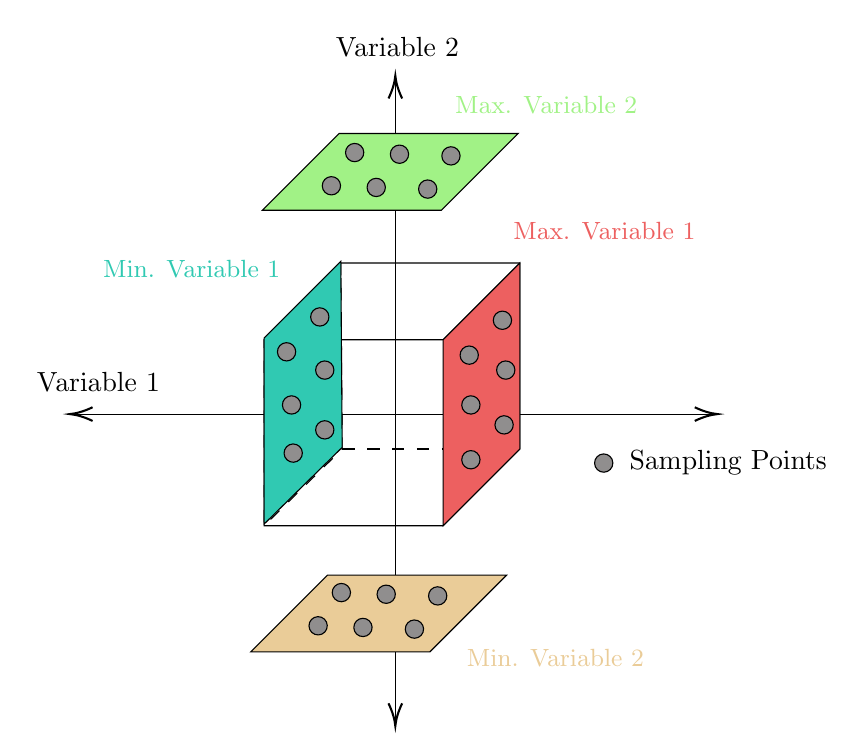
\begin{tikzpicture}[x=0.75pt,y=0.75pt,yscale=-1,xscale=1]
%uncomment if require: \path (0,426); %set diagram left start at 0, and has height of 426

%Shape: Cube [id:dp41916472639407576] 
\draw   (188.8,213.17) -- (225.77,176.2) -- (312.03,176.2) -- (312.03,265.83) -- (275.06,302.8) -- (188.8,302.8) -- cycle ; \draw   (312.03,176.2) -- (275.06,213.17) -- (188.8,213.17) ; \draw   (275.06,213.17) -- (275.06,302.8) ;
%Straight Lines [id:da1100678834838219] 
\draw    (254.4,249) -- (405.23,249) ;
\draw [shift={(407.23,249)}, rotate = 180] [color={rgb, 255:red, 0; green, 0; blue, 0 }  ][line width=0.75]    (10.93,-3.29) .. controls (6.95,-1.4) and (3.31,-0.3) .. (0,0) .. controls (3.31,0.3) and (6.95,1.4) .. (10.93,3.29)   ;
%Straight Lines [id:da8209310669516441] 
\draw    (254.4,249) -- (97.23,249) ;
\draw [shift={(95.23,249)}, rotate = 360] [color={rgb, 255:red, 0; green, 0; blue, 0 }  ][line width=0.75]    (10.93,-3.29) .. controls (6.95,-1.4) and (3.31,-0.3) .. (0,0) .. controls (3.31,0.3) and (6.95,1.4) .. (10.93,3.29)   ;
%Shape: Polygon [id:ds315102272045769] 
\draw  [dash pattern={on 4.5pt off 4.5pt}] (225.77,176.2) -- (226.43,265.83) -- (188.8,302.8) -- (188.8,213.17) -- cycle ;
%Straight Lines [id:da6924249131024756] 
\draw  [dash pattern={on 4.5pt off 4.5pt}]  (226.43,265.83) -- (312.03,265.83) ;
%Shape: Polygon [id:ds26648827466781355] 
\draw  [fill={rgb, 255:red, 237; green, 96; blue, 96 }  ,fill opacity=1 ] (312.03,176.2) -- (312.03,265.83) -- (275.06,302.8) -- (275.06,213.17) -- cycle ;
%Shape: Polygon [id:ds5376783951801227] 
\draw  [fill={rgb, 255:red, 48; green, 201; blue, 178 }  ,fill opacity=1 ] (225.77,175.4) -- (226.43,265.03) -- (188.8,302) -- (188.8,212.37) -- cycle ;
%Shape: Circle [id:dp6613928021845482] 
\draw  [fill={rgb, 255:red, 144; green, 142; blue, 142 }  ,fill opacity=1 ] (211.23,202.31) .. controls (211.16,199.88) and (213.08,197.85) .. (215.51,197.79) .. controls (217.95,197.72) and (219.97,199.64) .. (220.04,202.07) .. controls (220.1,204.51) and (218.19,206.53) .. (215.75,206.6) .. controls (213.32,206.66) and (211.29,204.75) .. (211.23,202.31) -- cycle ;
%Shape: Circle [id:dp10792302470599302] 
\draw  [fill={rgb, 255:red, 144; green, 142; blue, 142 }  ,fill opacity=1 ] (195.23,219.11) .. controls (195.16,216.68) and (197.08,214.65) .. (199.51,214.59) .. controls (201.95,214.52) and (203.97,216.44) .. (204.04,218.87) .. controls (204.1,221.31) and (202.19,223.33) .. (199.75,223.4) .. controls (197.32,223.46) and (195.29,221.55) .. (195.23,219.11) -- cycle ;
%Shape: Circle [id:dp764393572474829] 
\draw  [fill={rgb, 255:red, 144; green, 142; blue, 142 }  ,fill opacity=1 ] (213.63,227.91) .. controls (213.56,225.48) and (215.48,223.45) .. (217.91,223.39) .. controls (220.35,223.32) and (222.37,225.24) .. (222.44,227.67) .. controls (222.5,230.11) and (220.59,232.13) .. (218.15,232.2) .. controls (215.72,232.26) and (213.69,230.35) .. (213.63,227.91) -- cycle ;
%Shape: Circle [id:dp2635654509882438] 
\draw  [fill={rgb, 255:red, 144; green, 142; blue, 142 }  ,fill opacity=1 ] (197.63,244.71) .. controls (197.56,242.28) and (199.48,240.25) .. (201.91,240.19) .. controls (204.35,240.12) and (206.37,242.04) .. (206.44,244.47) .. controls (206.5,246.91) and (204.59,248.93) .. (202.15,249) .. controls (199.72,249.06) and (197.69,247.15) .. (197.63,244.71) -- cycle ;
%Shape: Circle [id:dp720401298117804] 
\draw  [fill={rgb, 255:red, 144; green, 142; blue, 142 }  ,fill opacity=1 ] (213.63,256.71) .. controls (213.56,254.28) and (215.48,252.25) .. (217.91,252.19) .. controls (220.35,252.12) and (222.37,254.04) .. (222.44,256.47) .. controls (222.5,258.91) and (220.59,260.93) .. (218.15,261) .. controls (215.72,261.06) and (213.69,259.15) .. (213.63,256.71) -- cycle ;
%Shape: Circle [id:dp3334941876745968] 
\draw  [fill={rgb, 255:red, 144; green, 142; blue, 142 }  ,fill opacity=1 ] (198.43,267.91) .. controls (198.36,265.48) and (200.28,263.45) .. (202.71,263.39) .. controls (205.15,263.32) and (207.17,265.24) .. (207.24,267.67) .. controls (207.3,270.11) and (205.39,272.13) .. (202.95,272.2) .. controls (200.52,272.26) and (198.49,270.35) .. (198.43,267.91) -- cycle ;
%Shape: Circle [id:dp9121056350905267] 
\draw  [fill={rgb, 255:red, 144; green, 142; blue, 142 }  ,fill opacity=1 ] (299.23,203.91) .. controls (299.16,201.48) and (301.08,199.45) .. (303.51,199.39) .. controls (305.95,199.32) and (307.97,201.24) .. (308.04,203.67) .. controls (308.1,206.11) and (306.19,208.13) .. (303.75,208.2) .. controls (301.32,208.26) and (299.29,206.35) .. (299.23,203.91) -- cycle ;
%Shape: Circle [id:dp461002915724564] 
\draw  [fill={rgb, 255:red, 144; green, 142; blue, 142 }  ,fill opacity=1 ] (283.23,220.71) .. controls (283.16,218.28) and (285.08,216.25) .. (287.51,216.19) .. controls (289.95,216.12) and (291.97,218.04) .. (292.04,220.47) .. controls (292.1,222.91) and (290.19,224.93) .. (287.75,225) .. controls (285.32,225.06) and (283.29,223.15) .. (283.23,220.71) -- cycle ;
%Shape: Circle [id:dp715936866594871] 
\draw  [fill={rgb, 255:red, 144; green, 142; blue, 142 }  ,fill opacity=1 ] (300.83,227.91) .. controls (300.76,225.48) and (302.68,223.45) .. (305.11,223.39) .. controls (307.55,223.32) and (309.57,225.24) .. (309.64,227.67) .. controls (309.7,230.11) and (307.79,232.13) .. (305.35,232.2) .. controls (302.92,232.26) and (300.89,230.35) .. (300.83,227.91) -- cycle ;
%Shape: Circle [id:dp5335650842060755] 
\draw  [fill={rgb, 255:red, 144; green, 142; blue, 142 }  ,fill opacity=1 ] (284.03,244.71) .. controls (283.96,242.28) and (285.88,240.25) .. (288.31,240.19) .. controls (290.75,240.12) and (292.77,242.04) .. (292.84,244.47) .. controls (292.9,246.91) and (290.99,248.93) .. (288.55,249) .. controls (286.12,249.06) and (284.09,247.15) .. (284.03,244.71) -- cycle ;
%Shape: Circle [id:dp6761023350021587] 
\draw  [fill={rgb, 255:red, 144; green, 142; blue, 142 }  ,fill opacity=1 ] (300.03,254.31) .. controls (299.96,251.88) and (301.88,249.85) .. (304.31,249.79) .. controls (306.75,249.72) and (308.77,251.64) .. (308.84,254.07) .. controls (308.9,256.51) and (306.99,258.53) .. (304.55,258.6) .. controls (302.12,258.66) and (300.09,256.75) .. (300.03,254.31) -- cycle ;
%Shape: Circle [id:dp7779527390505632] 
\draw  [fill={rgb, 255:red, 144; green, 142; blue, 142 }  ,fill opacity=1 ] (284.03,271.11) .. controls (283.96,268.68) and (285.88,266.65) .. (288.31,266.59) .. controls (290.75,266.52) and (292.77,268.44) .. (292.84,270.87) .. controls (292.9,273.31) and (290.99,275.33) .. (288.55,275.4) .. controls (286.12,275.46) and (284.09,273.55) .. (284.03,271.11) -- cycle ;
%Shape: Circle [id:dp39193327346815965] 
\draw  [fill={rgb, 255:red, 144; green, 142; blue, 142 }  ,fill opacity=1 ] (348.03,272.71) .. controls (347.96,270.28) and (349.88,268.25) .. (352.31,268.19) .. controls (354.75,268.12) and (356.77,270.04) .. (356.84,272.47) .. controls (356.9,274.91) and (354.99,276.93) .. (352.55,277) .. controls (350.12,277.06) and (348.09,275.15) .. (348.03,272.71) -- cycle ;
%Straight Lines [id:da4370737882051544] 
\draw    (252.03,397.29) -- (252.03,88) ;
\draw [shift={(252.03,86)}, rotate = 90] [color={rgb, 255:red, 0; green, 0; blue, 0 }  ][line width=0.75]    (10.93,-3.29) .. controls (6.95,-1.4) and (3.31,-0.3) .. (0,0) .. controls (3.31,0.3) and (6.95,1.4) .. (10.93,3.29)   ;
\draw [shift={(252.03,399.29)}, rotate = 270] [color={rgb, 255:red, 0; green, 0; blue, 0 }  ][line width=0.75]    (10.93,-3.29) .. controls (6.95,-1.4) and (3.31,-0.3) .. (0,0) .. controls (3.31,0.3) and (6.95,1.4) .. (10.93,3.29)   ;
%Shape: Polygon [id:ds027192625551482386] 
\draw  [fill={rgb, 255:red, 161; green, 242; blue, 134 }  ,fill opacity=1 ] (311.23,113.8) -- (274.26,150.77) -- (188,150.77) -- (224.97,113.8) -- cycle ;
%Shape: Polygon [id:ds7003641159858384] 
\draw  [fill={rgb, 255:red, 234; green, 204; blue, 152 }  ,fill opacity=1 ] (305.63,326.6) -- (268.66,363.57) -- (182.4,363.57) -- (219.37,326.6) -- cycle ;
%Shape: Circle [id:dp7862884715493691] 
\draw  [fill={rgb, 255:red, 144; green, 142; blue, 142 }  ,fill opacity=1 ] (228.03,123.11) .. controls (227.96,120.68) and (229.88,118.65) .. (232.31,118.59) .. controls (234.75,118.52) and (236.77,120.44) .. (236.84,122.87) .. controls (236.9,125.31) and (234.99,127.33) .. (232.55,127.4) .. controls (230.12,127.46) and (228.09,125.55) .. (228.03,123.11) -- cycle ;
%Shape: Circle [id:dp9269233874737624] 
\draw  [fill={rgb, 255:red, 144; green, 142; blue, 142 }  ,fill opacity=1 ] (216.83,139.11) .. controls (216.76,136.68) and (218.68,134.65) .. (221.11,134.59) .. controls (223.55,134.52) and (225.57,136.44) .. (225.64,138.87) .. controls (225.7,141.31) and (223.79,143.33) .. (221.35,143.4) .. controls (218.92,143.46) and (216.89,141.55) .. (216.83,139.11) -- cycle ;
%Shape: Circle [id:dp9900121536496537] 
\draw  [fill={rgb, 255:red, 144; green, 142; blue, 142 }  ,fill opacity=1 ] (249.63,123.91) .. controls (249.56,121.48) and (251.48,119.45) .. (253.91,119.39) .. controls (256.35,119.32) and (258.37,121.24) .. (258.44,123.67) .. controls (258.5,126.11) and (256.59,128.13) .. (254.15,128.2) .. controls (251.72,128.26) and (249.69,126.35) .. (249.63,123.91) -- cycle ;
%Shape: Circle [id:dp0010559062693412669] 
\draw  [fill={rgb, 255:red, 144; green, 142; blue, 142 }  ,fill opacity=1 ] (238.43,139.91) .. controls (238.36,137.48) and (240.28,135.45) .. (242.71,135.39) .. controls (245.15,135.32) and (247.17,137.24) .. (247.24,139.67) .. controls (247.3,142.11) and (245.39,144.13) .. (242.95,144.2) .. controls (240.52,144.26) and (238.49,142.35) .. (238.43,139.91) -- cycle ;
%Shape: Circle [id:dp9729939432021396] 
\draw  [fill={rgb, 255:red, 144; green, 142; blue, 142 }  ,fill opacity=1 ] (274.43,124.71) .. controls (274.36,122.28) and (276.28,120.25) .. (278.71,120.19) .. controls (281.15,120.12) and (283.17,122.04) .. (283.24,124.47) .. controls (283.3,126.91) and (281.39,128.93) .. (278.95,129) .. controls (276.52,129.06) and (274.49,127.15) .. (274.43,124.71) -- cycle ;
%Shape: Circle [id:dp5583563494601032] 
\draw  [fill={rgb, 255:red, 144; green, 142; blue, 142 }  ,fill opacity=1 ] (263.23,140.71) .. controls (263.16,138.28) and (265.08,136.25) .. (267.51,136.19) .. controls (269.95,136.12) and (271.97,138.04) .. (272.04,140.47) .. controls (272.1,142.91) and (270.19,144.93) .. (267.75,145) .. controls (265.32,145.06) and (263.29,143.15) .. (263.23,140.71) -- cycle ;
%Shape: Circle [id:dp2803403187081903] 
\draw  [fill={rgb, 255:red, 144; green, 142; blue, 142 }  ,fill opacity=1 ] (221.63,335.11) .. controls (221.56,332.68) and (223.48,330.65) .. (225.91,330.59) .. controls (228.35,330.52) and (230.37,332.44) .. (230.44,334.87) .. controls (230.5,337.31) and (228.59,339.33) .. (226.15,339.4) .. controls (223.72,339.46) and (221.69,337.55) .. (221.63,335.11) -- cycle ;
%Shape: Circle [id:dp08580816994108764] 
\draw  [fill={rgb, 255:red, 144; green, 142; blue, 142 }  ,fill opacity=1 ] (210.43,351.11) .. controls (210.36,348.68) and (212.28,346.65) .. (214.71,346.59) .. controls (217.15,346.52) and (219.17,348.44) .. (219.24,350.87) .. controls (219.3,353.31) and (217.39,355.33) .. (214.95,355.4) .. controls (212.52,355.46) and (210.49,353.55) .. (210.43,351.11) -- cycle ;
%Shape: Circle [id:dp8920356550311489] 
\draw  [fill={rgb, 255:red, 144; green, 142; blue, 142 }  ,fill opacity=1 ] (243.23,335.91) .. controls (243.16,333.48) and (245.08,331.45) .. (247.51,331.39) .. controls (249.95,331.32) and (251.97,333.24) .. (252.04,335.67) .. controls (252.1,338.11) and (250.19,340.13) .. (247.75,340.2) .. controls (245.32,340.26) and (243.29,338.35) .. (243.23,335.91) -- cycle ;
%Shape: Circle [id:dp9149486091931166] 
\draw  [fill={rgb, 255:red, 144; green, 142; blue, 142 }  ,fill opacity=1 ] (232.03,351.91) .. controls (231.96,349.48) and (233.88,347.45) .. (236.31,347.39) .. controls (238.75,347.32) and (240.77,349.24) .. (240.84,351.67) .. controls (240.9,354.11) and (238.99,356.13) .. (236.55,356.2) .. controls (234.12,356.26) and (232.09,354.35) .. (232.03,351.91) -- cycle ;
%Shape: Circle [id:dp453151861693878] 
\draw  [fill={rgb, 255:red, 144; green, 142; blue, 142 }  ,fill opacity=1 ] (268.03,336.71) .. controls (267.96,334.28) and (269.88,332.25) .. (272.31,332.19) .. controls (274.75,332.12) and (276.77,334.04) .. (276.84,336.47) .. controls (276.9,338.91) and (274.99,340.93) .. (272.55,341) .. controls (270.12,341.06) and (268.09,339.15) .. (268.03,336.71) -- cycle ;
%Shape: Circle [id:dp2654623156037197] 
\draw  [fill={rgb, 255:red, 144; green, 142; blue, 142 }  ,fill opacity=1 ] (256.83,352.71) .. controls (256.76,350.28) and (258.68,348.25) .. (261.11,348.19) .. controls (263.55,348.12) and (265.57,350.04) .. (265.64,352.47) .. controls (265.7,354.91) and (263.79,356.93) .. (261.35,357) .. controls (258.92,357.06) and (256.89,355.15) .. (256.83,352.71) -- cycle ;

% Text Node
\draw (108.99,233.5) node   [align=left] {Variable 1};
% Text Node
\draw (279.6,94.6) node [anchor=north west][inner sep=0.75pt]  [font=\small,color={rgb, 255:red, 161; green, 242; blue, 134 }  ,opacity=1 ] [align=left] {Max. Variable 2};
% Text Node
\draw (307.6,155.4) node [anchor=north west][inner sep=0.75pt]  [font=\small,color={rgb, 255:red, 237; green, 96; blue, 96 }  ,opacity=1 ] [align=left] {Max. Variable 1};
% Text Node
\draw (363.6,265.4) node [anchor=north west][inner sep=0.75pt]   [align=left] {Sampling Points};
% Text Node
\draw (252.99,71.9) node   [align=left] {Variable 2};
% Text Node
\draw (110,173.8) node [anchor=north west][inner sep=0.75pt]  [font=\small,color={rgb, 255:red, 48; green, 201; blue, 178 }  ,opacity=1 ] [align=left] {Min. Variable 1};
% Text Node
\draw (285.2,361) node [anchor=north west][inner sep=0.75pt]  [font=\small,color={rgb, 255:red, 234; green, 204; blue, 152 }  ,opacity=1 ] [align=left] {Min. Variable 2};

\end{tikzpicture}
\caption{Data sampling strategy following a Latin Hypercube approach. The minimum and maximum value for each variable is fixed and $n$ data points are chosen, which creates $n_{variables}\times n_{points}\times 2$ experiments}
\label{fig: hypercube}
\end{figure}



By using $n$ number of design variables, this concept expands to an $n$-dimensional hypercube. This allows us to explore a broader design space, making sure that every point data is meaningful, as it represents a unique combination of potentials. In this paper, we utilized 25 sampling points, ie: there are 25 data points in each of the faces of the cube, creating $4\times 25 \times 2=200$ different combinations of potentials.

These potentials will be used as an input for the finite element analysis, in the form of a 4-element vector (the potential at each electrode). Moreover, since 200 experiments will likely be unsufficient to capture the complex phenomena behind this dielectric elastomer using a machine learning model, we will enrich this data further. To do so, we will take advantage of the load-stepping scheme implemented in the finite element analysis. Load-stepping allows for an easier convergence of the Newton-Raphson algorithm. By applying a fraction of the total load at the beginning of the analysis, solving the Newton-Raphson and then increasing the load, we can better capture non-linearities, increasing convergence. 

Utilizing these intermediate data, we can extend the initial 200 finite element samples, to over 20000, accounting for possible cutbacks and bisections during the load-stepping, which will further increase the data available. For each load (combination of potentials), we also needed to store the displacement output. For ease of access and convenience, we projected the displacement of all the nodes to one of the top surfaces of the dielectric elastomer, which contains 133 nodes. Hence, for each 4-element vector load, we will have a corresponding 399-element vector of displacement (coordinates 1, 2 and 3 of each of the 133 points). These will be our training and test samples.


\subsubsection{Training strategy}

The goal now is to train a neural network to accurately predict the displacement of the dielectric elastomer for a given input potential. Hence, the input for the neural network is a 4-element vector and the output is a 399-element vector. However, since the primary deformation mechanisms will be bending and torsion, the effect of shear deformation is negligible. This allows us to effectively remove one of the components of the displacements, namely the one that represents the movement in axial direction. As a result, the original 399-element data is reduced to 266-element data, which holds only displacements in the first and third coordinate directions. 

Using this data, we can train a neural network that predicts the displacement for a given combination of potentials. However, the proper architecture to do this prediction is unknown at this stage. There is no clear direction in which the hyperparemeters of the neural network need to be changed in order to achieve reasonable prediction capabilities. For this reason, a parametric study was carried out in which neural network calibration is done by varying different hyperparameter values. Namely: the number of nodes ($n_{nodes}$), the number of neurons ($n_{neurons}$), the number of experiments ($n_{experiments}$) and the number of layers ($n_{layers}$). To study the convergence of the machine learning model, the number of epochs was also introduced in the parametric study.



\tikzset{every picture/.style={line width=0.75pt}} %set default line width to 0.75pt        
\begin{figure}
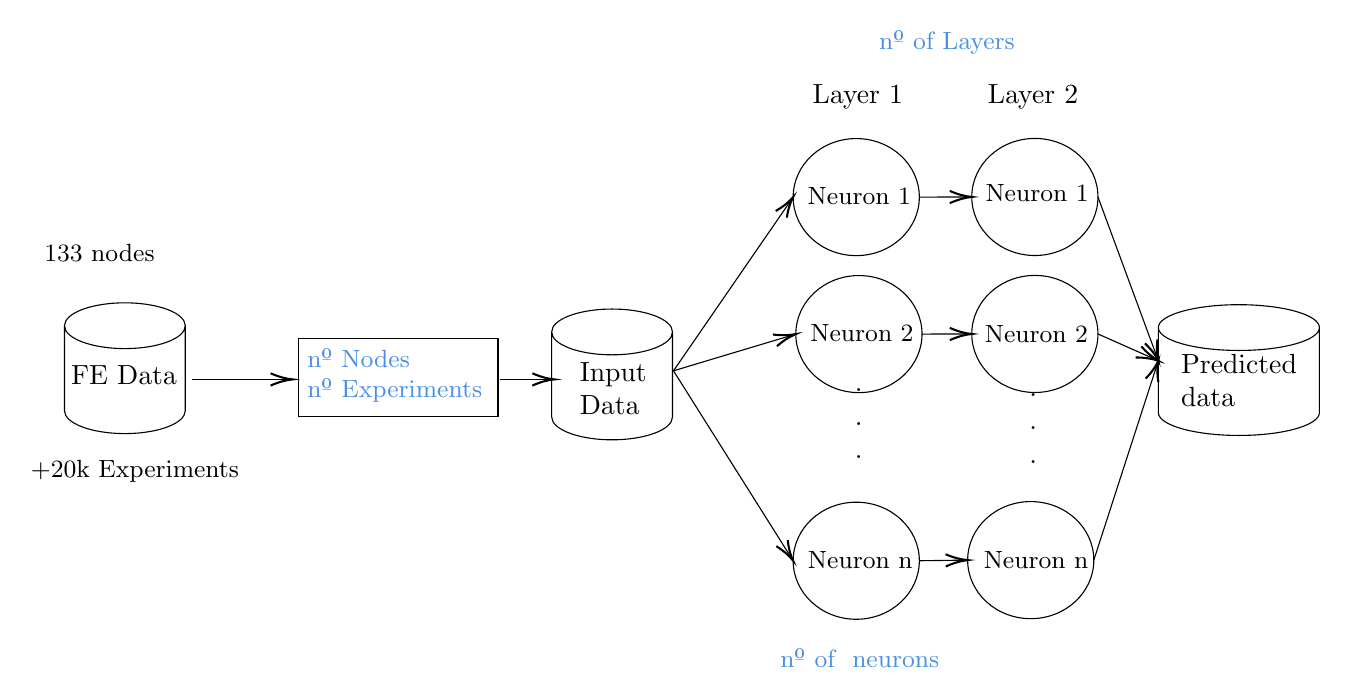
\begin{tikzpicture}[x=0.75pt,y=0.75pt,yscale=-0.9,xscale=0.97]
%uncomment if require: \path (0,444); %set diagram left start at 0, and has height of 444

%Shape: Circle [id:dp7149132561338333] 
\draw   (388.61,102.4) .. controls (388.61,85.1) and (402.64,71.07) .. (419.94,71.07) .. controls (437.25,71.07) and (451.28,85.1) .. (451.28,102.4) .. controls (451.28,119.7) and (437.25,133.73) .. (419.94,133.73) .. controls (402.64,133.73) and (388.61,119.7) .. (388.61,102.4) -- cycle ;
%Shape: Circle [id:dp013523830492098043] 
\draw   (389.94,175.73) .. controls (389.94,158.43) and (403.97,144.4) .. (421.28,144.4) .. controls (438.58,144.4) and (452.61,158.43) .. (452.61,175.73) .. controls (452.61,193.04) and (438.58,207.07) .. (421.28,207.07) .. controls (403.97,207.07) and (389.94,193.04) .. (389.94,175.73) -- cycle ;
%Shape: Circle [id:dp6349374096098536] 
\draw   (388.61,297.07) .. controls (388.61,279.76) and (402.64,265.73) .. (419.94,265.73) .. controls (437.25,265.73) and (451.28,279.76) .. (451.28,297.07) .. controls (451.28,314.37) and (437.25,328.4) .. (419.94,328.4) .. controls (402.64,328.4) and (388.61,314.37) .. (388.61,297.07) -- cycle ;
%Flowchart: Magnetic Disk [id:dp2804160649676165] 
\draw   (86.67,171.25) -- (86.67,216.75) .. controls (86.67,223.52) and (73.24,229) .. (56.67,229) .. controls (40.1,229) and (26.67,223.52) .. (26.67,216.75) -- (26.67,171.25)(86.67,171.25) .. controls (86.67,178.02) and (73.24,183.5) .. (56.67,183.5) .. controls (40.1,183.5) and (26.67,178.02) .. (26.67,171.25) .. controls (26.67,164.48) and (40.1,159) .. (56.67,159) .. controls (73.24,159) and (86.67,164.48) .. (86.67,171.25) -- cycle ;
%Flowchart: Magnetic Disk [id:dp6592793249759878] 
\draw   (328.67,174.58) -- (328.67,220.08) .. controls (328.67,226.85) and (315.24,232.33) .. (298.67,232.33) .. controls (282.1,232.33) and (268.67,226.85) .. (268.67,220.08) -- (268.67,174.58)(328.67,174.58) .. controls (328.67,181.35) and (315.24,186.83) .. (298.67,186.83) .. controls (282.1,186.83) and (268.67,181.35) .. (268.67,174.58) .. controls (268.67,167.82) and (282.1,162.33) .. (298.67,162.33) .. controls (315.24,162.33) and (328.67,167.82) .. (328.67,174.58) -- cycle ;
%Straight Lines [id:da35532704073807175] 
\draw    (387.53,104.09) -- (329.17,195.39) ;
\draw [shift={(388.61,102.4)}, rotate = 122.59] [color={rgb, 255:red, 0; green, 0; blue, 0 }  ][line width=0.75]    (10.93,-3.29) .. controls (6.95,-1.4) and (3.31,-0.3) .. (0,0) .. controls (3.31,0.3) and (6.95,1.4) .. (10.93,3.29)   ;
%Straight Lines [id:da4511032574004499] 
\draw    (388.04,176.35) -- (329.17,195.39) ;
\draw [shift={(389.94,175.73)}, rotate = 162.08] [color={rgb, 255:red, 0; green, 0; blue, 0 }  ][line width=0.75]    (10.93,-3.29) .. controls (6.95,-1.4) and (3.31,-0.3) .. (0,0) .. controls (3.31,0.3) and (6.95,1.4) .. (10.93,3.29)   ;
%Straight Lines [id:da19079915385094404] 
\draw    (387.6,295.34) -- (329.17,195.39) ;
\draw [shift={(388.61,297.07)}, rotate = 239.69] [color={rgb, 255:red, 0; green, 0; blue, 0 }  ][line width=0.75]    (10.93,-3.29) .. controls (6.95,-1.4) and (3.31,-0.3) .. (0,0) .. controls (3.31,0.3) and (6.95,1.4) .. (10.93,3.29)   ;
%Shape: Circle [id:dp7482248959951554] 
\draw   (477.33,102.33) .. controls (477.33,85.03) and (491.36,71) .. (508.67,71) .. controls (525.97,71) and (540,85.03) .. (540,102.33) .. controls (540,119.64) and (525.97,133.67) .. (508.67,133.67) .. controls (491.36,133.67) and (477.33,119.64) .. (477.33,102.33) -- cycle ;
%Shape: Circle [id:dp5965819972858774] 
\draw   (477.33,175.67) .. controls (477.33,158.36) and (491.36,144.33) .. (508.67,144.33) .. controls (525.97,144.33) and (540,158.36) .. (540,175.67) .. controls (540,192.97) and (525.97,207) .. (508.67,207) .. controls (491.36,207) and (477.33,192.97) .. (477.33,175.67) -- cycle ;
%Shape: Circle [id:dp5648862567333319] 
\draw   (475.28,296.73) .. controls (475.28,279.43) and (489.31,265.4) .. (506.61,265.4) .. controls (523.92,265.4) and (537.94,279.43) .. (537.94,296.73) .. controls (537.94,314.04) and (523.92,328.07) .. (506.61,328.07) .. controls (489.31,328.07) and (475.28,314.04) .. (475.28,296.73) -- cycle ;
%Straight Lines [id:da8586261828242774] 
\draw    (451.28,102.4) -- (475.33,102.34) ;
\draw [shift={(477.33,102.33)}, rotate = 179.85] [color={rgb, 255:red, 0; green, 0; blue, 0 }  ][line width=0.75]    (10.93,-3.29) .. controls (6.95,-1.4) and (3.31,-0.3) .. (0,0) .. controls (3.31,0.3) and (6.95,1.4) .. (10.93,3.29)   ;
%Straight Lines [id:da7717426599628258] 
\draw    (452.61,175.73) -- (475.33,175.67) ;
\draw [shift={(477.33,175.67)}, rotate = 179.85] [color={rgb, 255:red, 0; green, 0; blue, 0 }  ][line width=0.75]    (10.93,-3.29) .. controls (6.95,-1.4) and (3.31,-0.3) .. (0,0) .. controls (3.31,0.3) and (6.95,1.4) .. (10.93,3.29)   ;
%Straight Lines [id:da3046916071479544] 
\draw    (451.28,297.07) -- (473.28,296.76) ;
\draw [shift={(475.28,296.73)}, rotate = 179.2] [color={rgb, 255:red, 0; green, 0; blue, 0 }  ][line width=0.75]    (10.93,-3.29) .. controls (6.95,-1.4) and (3.31,-0.3) .. (0,0) .. controls (3.31,0.3) and (6.95,1.4) .. (10.93,3.29)   ;
%Straight Lines [id:da6640975488428904] 
\draw    (90,200) -- (138,200) ;
\draw [shift={(140,200)}, rotate = 180] [color={rgb, 255:red, 0; green, 0; blue, 0 }  ][line width=0.75]    (10.93,-3.29) .. controls (6.95,-1.4) and (3.31,-0.3) .. (0,0) .. controls (3.31,0.3) and (6.95,1.4) .. (10.93,3.29)   ;
%Straight Lines [id:da6892392743456469] 
\draw    (243,200) -- (268,200) ;
\draw [shift={(270,200)}, rotate = 180] [color={rgb, 255:red, 0; green, 0; blue, 0 }  ][line width=0.75]    (10.93,-3.29) .. controls (6.95,-1.4) and (3.31,-0.3) .. (0,0) .. controls (3.31,0.3) and (6.95,1.4) .. (10.93,3.29)   ;
%Flowchart: Magnetic Disk [id:dp35749579079078997] 
\draw   (650,172.25) -- (650,217.75) .. controls (650,224.52) and (632.09,230) .. (610,230) .. controls (587.91,230) and (570,224.52) .. (570,217.75) -- (570,172.25)(650,172.25) .. controls (650,179.02) and (632.09,184.5) .. (610,184.5) .. controls (587.91,184.5) and (570,179.02) .. (570,172.25) .. controls (570,165.48) and (587.91,160) .. (610,160) .. controls (632.09,160) and (650,165.48) .. (650,172.25) -- cycle ;
%Straight Lines [id:da5896782313243266] 
\draw    (540,102.33) -- (569.35,188.11) ;
\draw [shift={(570,190)}, rotate = 251.11] [color={rgb, 255:red, 0; green, 0; blue, 0 }  ][line width=0.75]    (10.93,-3.29) .. controls (6.95,-1.4) and (3.31,-0.3) .. (0,0) .. controls (3.31,0.3) and (6.95,1.4) .. (10.93,3.29)   ;
%Straight Lines [id:da28421655439140037] 
\draw    (540,175.67) -- (568.2,189.14) ;
\draw [shift={(570,190)}, rotate = 205.54] [color={rgb, 255:red, 0; green, 0; blue, 0 }  ][line width=0.75]    (10.93,-3.29) .. controls (6.95,-1.4) and (3.31,-0.3) .. (0,0) .. controls (3.31,0.3) and (6.95,1.4) .. (10.93,3.29)   ;
%Straight Lines [id:da846956632663103] 
\draw    (537.94,296.73) -- (569.42,191.92) ;
\draw [shift={(570,190)}, rotate = 106.72] [color={rgb, 255:red, 0; green, 0; blue, 0 }  ][line width=0.75]    (10.93,-3.29) .. controls (6.95,-1.4) and (3.31,-0.3) .. (0,0) .. controls (3.31,0.3) and (6.95,1.4) .. (10.93,3.29)   ;

% Text Node
\draw (422.79,175.12) node  [font=\small] [align=left] {Neuron 2};
% Text Node
\draw (421.94,296.94) node  [font=\small] [align=left] {Neuron n};
% Text Node
\draw (418,203.67) node [anchor=north west][inner sep=0.75pt]   [align=left] {.\\.\\.};
% Text Node
\draw (28.67,191.33) node [anchor=north west][inner sep=0.75pt]   [align=left] {FE Data};
% Text Node
\draw    (143,178) -- (242,178) -- (242,220) -- (143,220) -- cycle  ;
\draw (146,182) node [anchor=north west][inner sep=0.75pt]  [font=\small,color={rgb, 255:red, 74; green, 144; blue, 226 }  ,opacity=1 ] [align=left] {nº Nodes\\nº Experiments};
% Text Node
\draw (15.33,126) node [anchor=north west][inner sep=0.75pt]  [font=\small,color={rgb, 255:red, 0; green, 0; blue, 0 }  ,opacity=1 ] [align=left] {133 nodes};
% Text Node
\draw (8.67,242) node [anchor=north west][inner sep=0.75pt]  [font=\small] [align=left] {+20k Experiments};
% Text Node
\draw (281.33,189.33) node [anchor=north west][inner sep=0.75pt]   [align=left] {Input \\Data};
% Text Node
\draw (509.46,175.78) node  [font=\small] [align=left] {Neuron 2};
% Text Node
\draw (509.28,296.94) node  [font=\small] [align=left] {Neuron n};
% Text Node
\draw (504.67,206.33) node [anchor=north west][inner sep=0.75pt]   [align=left] {.\\.\\.};
% Text Node
\draw (421.46,101.78) node  [font=\small] [align=left] {Neuron 1};
% Text Node
\draw (509.79,100.45) node  [font=\small] [align=left] {Neuron 1};
% Text Node
\draw (397,41) node [anchor=north west][inner sep=0.75pt]   [align=left] {Layer 1};
% Text Node
\draw (484,41) node [anchor=north west][inner sep=0.75pt]   [align=left] {Layer 2};
% Text Node
\draw (580,185) node [anchor=north west][inner sep=0.75pt]   [align=left] {Predicted \\data\\};
% Text Node
\draw (430,12) node [anchor=north west][inner sep=0.75pt]  [font=\small,color={rgb, 255:red, 74; green, 144; blue, 226 }  ,opacity=1 ] [align=left] {nº of Layers};
% Text Node
\draw (381,343) node [anchor=north west][inner sep=0.75pt]  [font=\small,color={rgb, 255:red, 74; green, 144; blue, 226 }  ,opacity=1 ] [align=left] {nº of \ neurons};


\end{tikzpicture}
\caption{Training process schematic. The number of variables modified during the parametric study can be seen in blue.}
\end{figure}
Alongside architecture-specific parameters, like the number of neurons, the number of layers and the number of epochs, we also studied the effect of the number of nodes and experiments. From the available 266 nodes, we took only a subset of them and used them to train the neural network, leaving the remaining nodes as test data to compare against. The same concept is used by selecting only a subset of experiments out of the ones available. The purpose of this subset selection is calibrating a neural network that is able to predict the complete response, reducing the computational expense without losing accuracy by reducing the number of nodes and experiments used. 

For each of the hyperparameters specified, the values studied were the following:

\begin{table}[!hb]
  \centering
\begin{tabular}{l|cccc}
\textbf{Parameters} & \multicolumn{3}{c}{\textbf{Value}} \\ \hline
Layers              & 4      & 8       & 10            \\
Neurons             & 10     & 20      & 40           \\
Experiments         & 2077    & 7000    & 10000      \\
Nodes               & 50     & 10      & 200           \\
Epochs              &  \multicolumn{3}{c}{1e4}        
\end{tabular}
  \caption{Values used in the parametric study during the training phase. Every combination of these parameters was analysed and parsed to obtain the best performing architecture.}
\end{table}

\subsubsection{Results}


Every possible combination of these parameters was studied, totalling 80 different architectures that were run and analysed. To measure the performance of these architecture, the R2 measurement (\ref{eq:R2_measurement}), was used. This metric allows us to compare the displacements predicted by the neural network against the test data (the remaining data that was not taken into the training process). To provide a clearer outlook on the results of the parametric hyperparameter study, we compiled the output of R2 measurements on every combination of 50 and 200 nodes using 2077 and 10000 experiments. These results can be visualized in Table \ref{tab: R2_measurement}


% I will take 4 combinations of n_nodes and n_experiments



% n_nodes = 10
% n_experiments=4000
% iter = 5000

%n_nodes = 10 
% n_experiments=2000
% iter = 5000


%n_nodes = 30 
% n_experiments=4000
% iter = 5000

%n_nodes = 30 
% n_experiments=2000
% iter = 5000

% Please add the following required packages to your document preamble:
% \usepackage{multirow}
% Please add the following required packages to your document preamble:
% \usepackage{multirow}
\begin{table}[!hb]
\centering
\begin{minipage}{.49\textwidth}

\begin{tabular}{lllllllcc|ccc}
\multicolumn{9}{c|}{\multirow{2}{*}{\begin{tabular}[c]{@{}c@{}}$n_{nodes}=50$\\ $n_{experiments}=2077$\end{tabular}}} & \multicolumn{3}{c}{$n_{neurons}$} \\
\multicolumn{9}{c|}{}                                                                                                 & 10        & 20        & 40        \\ \hline
        &         &         &         &         &         &         & \multirow{4}{*}{\rotatebox{90}{$n_{layers}$}}        & 4        &  0.9969        &  0.9971        &  0.9990        \\
        &         &         &         &         &         &         &                                      & 8        &  0.9960        &  0.9985       &  0.9973        \\
        &         &         &         &         &         &         &                                      & 10        &  0.9970        &  0.9985        &  0.9990        
\end{tabular}

\end{minipage}

\begin{minipage}{.49\textwidth}

\begin{tabular}{lllllllcc|ccc}
\multicolumn{9}{c|}{\multirow{2}{*}{\begin{tabular}[c]{@{}c@{}}$n_{nodes}=50$\\ $n_{experiments}=10000$\end{tabular}}} & \multicolumn{3}{c}{$n_{neurons}$} \\
\multicolumn{9}{c|}{}                                                                                                 & 10        & 20        & 40        \\ \hline
        &         &         &         &         &         &         & \multirow{4}{*}{\rotatebox{90}{$n_{layers}$}}        & 4        &  0.9953        &  0.9986        &  0.9989        \\
        &         &         &         &         &         &         &                                      & 8        &  0.9968        &  0.9982       &  0.9987        \\
        &         &         &         &         &         &         &                                      & 10        &  0.9965        &  0.9983        &  0.9990        
\end{tabular}

\end{minipage}

\begin{minipage}{.49\textwidth}

\begin{tabular}{lllllllcc|ccc}
\multicolumn{9}{c|}{\multirow{2}{*}{\begin{tabular}[c]{@{}c@{}}$n_{nodes}=200$\\ $n_{experiments}=2077$\end{tabular}}} & \multicolumn{3}{c}{$n_{neurons}$} \\
\multicolumn{9}{c|}{}                                                                                                 & 10        & 20        & 40        \\ \hline
        &         &         &         &         &         &         & \multirow{4}{*}{\rotatebox{90}{$n_{layers}$}}        & 4        &  0.9966        &  0.9980        &  0.9988        \\
        &         &         &         &         &         &         &                                      & 8        &  0.9962        &  0.9982       &  0.9984        \\
        &         &         &         &         &         &         &                                      & 10        &  0.9891        &  0.9978        &  0.9977        
\end{tabular}

\end{minipage}

\begin{minipage}{.49\textwidth}

\begin{tabular}{lllllllcc|ccc}
\multicolumn{9}{c|}{\multirow{2}{*}{\begin{tabular}[c]{@{}c@{}}$n_{nodes}=200$\\ $n_{experiments}=10000$\end{tabular}}} & \multicolumn{3}{c}{$n_{neurons}$} \\
\multicolumn{9}{c|}{}                                                                                                 & 10        & 20        & 40        \\ \hline
        &         &         &         &         &         &         & \multirow{4}{*}{\rotatebox{90}{$n_{layers}$}}        & 4        &  0.9944        &  0.9981        &  0.9991        \\
        &         &         &         &         &         &         &                                      & 8        &  0.9958        &  0.9976       &  0.9995        \\
        &         &         &         &         &         &         &                                      & 10        &  0.9971        &  0.9977        &  0.9969        
\end{tabular}

\end{minipage}





  \caption{R2 measurement for every combination of neurons and layers for 50 and 200 nodes and 2077 and 10000 experiments.}
  \label{tab: R2_values}
\end{table}


Out of the analysed architectures in Table \ref{tab: R2_values}, the best configuration is a combination of 8 layers, 40 neurons, 10000 experiments, 200 nodes  with an R2 on the test cases of 0.9995. 

To measure the dispersion of the data generated from the Machine Learning model against the in-silico FE data, we plotted the output displacement from the FE analysis against the displacement predicted by the Machine Learning architecture. Since the displacement data is given per axis in the global coordinate system, we compared the displacement per axis; namely the first and third axis. The output of this analysis is displayed in Figure \ref{fig: R2_plot} for various architectures tested.

\begin{figure}
  \centering
  \subfloat[Displacement in the first axis of the coordinate system of the best performing architecture: 8 layers | 40 neurons | 10000 experiments | 200 nodes]{\includegraphics[width=0.45\linewidth]{Figures/NeuralNetworkStudy/R2_Coord1_corrected_V3.pdf}} \qquad
  \subfloat[Displacement in the third axis of the coordinate system of the best performing architecture: 8 layers | 40 neurons | 10000 experiments | 200 nodes]{\includegraphics[width=0.45\linewidth]{Figures/NeuralNetworkStudy/R2_Coord3_corrected_V3.pdf}}\\
  \subfloat[Displacement in the first axis of the coordinate system of the architecture: 4 layers | 10 neurons | 2077 experiments | 50 nodes]{\includegraphics[width=0.45\linewidth]{Figures/NeuralNetworkStudy/R2_Coord1_corrected_V3_L4_N10_E2077_NN50.pdf}}\qquad
  \subfloat[Displacement in the third axis of the coordinate system of the architecture: 4 layers | 10 neurons | 2077 experiments | 50 nodes]{\includegraphics[width=0.45\linewidth]{Figures/NeuralNetworkStudy/R2_Coord3_corrected_V3_L4_N10_E2077_NN50.pdf}}\\
  \subfloat[Displacement in the first axis of the coordinate system of the architecture: 10 layers | 20 neurons | 2077 experiments | 50 nodes]{\includegraphics[width=0.45\linewidth]{Figures/NeuralNetworkStudy/R2_Coord1_corrected_V3_L10_N20_E2077_NN50.pdf}} \qquad
  \subfloat[Displacement in the third axis of the coordinate system of the architecture: 10 layers | 20 neurons | 2077 experiments | 50 nodes]{\includegraphics[width=0.45\linewidth]{Figures/NeuralNetworkStudy/R2_Coord3_corrected_V3_L10_N20_E2077_NN50.pdf}}\\
  \pagebreak
  \subfloat[Displacement in the first axis of the coordinate system of the architecture: 8 layers | 40 neurons | 2077 experiments | 200 nodes]{\includegraphics[width=0.45\linewidth]{Figures/NeuralNetworkStudy/R2_Coord1_corrected_V3_L8_N40_E2077_NN200.pdf}} \qquad
  \subfloat[Displacement in the third axis of the coordinate system of the architecture: 8 layers | 40 neurons | 2077 experiments | 200 nodes]{\includegraphics[width=0.45\linewidth]{Figures/NeuralNetworkStudy/R2_Coord3_corrected_V3_L8_N40_E2077_NN200.pdf}}
  \caption{R2 evaluation of the displacements. FE data vs ML predicted output for the better performing neural network architecture, and 3 other architectures. A clear linear distribution can be seen between the predicted and FE displacements, indicating a high R2 and correlation between the data. However, there is a dispersion in the data which can be expected due to the small amount of data taken as a training dataset.}
  \label{fig: R2_plot}
\end{figure}

As can be seen from Figure \ref{fig: R2_plot}, there is a high correlation between the predicted data from the neural network and the data coming from the FE analysis, which was also indicated by a high R2 value.

To further analyse the performance of the machine learning architecture, we can plot the loss function during the training process, which exhibits a downward tendency as the training progresses. This result can be seen in Figure \ref{fig: losses}. 


\begin{figure}
  \begin{center}
    \subfloat[Evolution of the loss function for the best performing architecture: 8 layers | 40 neurons | 10000 experiments | 200 nodes]{\includegraphics[width=0.45\linewidth]{Figures/NeuralNetworkStudy/Loss_corrected_V3.pdf}} \qquad
    \subfloat[Evolution of the loss function for the  architecture: 4 layers | 10 neurons | 2077 experiments | 50 nodes]{\includegraphics[width=0.45\linewidth]{Figures/NeuralNetworkStudy/Loss_corrected_V3_L4_N10_E2077_NN50.pdf}} \\
    \subfloat[Evolution of the loss function for the  architecture: 10 layers | 20 neurons | 2077 experiments | 50 nodes]{\includegraphics[width=0.45\linewidth]{Figures/NeuralNetworkStudy/Loss_corrected_V3_L10_N20_E2077_NN50.pdf}} \qquad
    \subfloat[Evolution of the loss function for the  architecture: 8 layers | 40 neurons | 2077 experiments | 200 nodes]{\includegraphics[width=0.45\linewidth]{Figures/NeuralNetworkStudy/Loss_corrected_V3_L8_N40_E2077_NN200.pdf}} 
  \end{center}
  \caption{Loss function during the training for the best performant neural network configuration, and 3 other architectures. Convergence is not fully achieved in every training architecture, however a high enough R2 is reached. This effectively means that further trainig the model would cause overfitting. Spikes can be seen in in the loss function during the training process, which are caused by a high value of the $\eta$ parameter in the Adam optimizer. This means that the loss is minimized quicker, at the expense of bigger fluctuating values. This strikes a good balance between effectiveness and precision.}
  \label{fig: losses}
\end{figure}


Besides the R2 measurement and scatter plot of predicted displacements versus FE generated data, we tracked the trajectory of certain points in the mesh throughout the deformation of the dielectric. By applying a combination of potentials in the electrodes and measuring the elastomer's response, we can compare that displacement against the one predicted by the neural network architecture. This can provide a better outlook on how accurately the machine learning model is predicting the real response of the dielectric. 


\begin{figure}
 \centering 
  \subfloat[Trajectory tracking of point 1 in the first axis of the coordinate system]{\includegraphics[width=0.45\linewidth]{Figures/NeuralNetworkStudy/Trajectory_03_009_0162_0066_P1_Coord1.pdf}}
  \subfloat[Trajectory tracking of point 1 in the third axis of the coordinate system]{\includegraphics[width=0.45\linewidth]{Figures/NeuralNetworkStudy/Trajectory_03_009_0162_0066_P1_Coord3.pdf}}\\
  \subfloat[Trajectory tracking of point 100 in the first axis of the coordinate system]{\includegraphics[width=0.45\linewidth]{Figures/NeuralNetworkStudy/Trajectory_03_009_0162_0066_P100_Coord1.pdf}}
  \subfloat[Trajectory tracking of point 100 in the third axis of the coordinate system]{\includegraphics[width=0.45\linewidth]{Figures/NeuralNetworkStudy/Trajectory_03_009_0162_0066_P100_Coord3.pdf}}\\
  \subfloat[Trajectory tracking of point 150 in the first axis of the coordinate system]{\includegraphics[width=0.45\linewidth]{Figures/NeuralNetworkStudy/Trajectory_03_009_0162_0066_P150_Coord1.pdf}}
  \subfloat[Trajectory tracking of point 150 in the third axis of the coordinate system]{\includegraphics[width=0.45\linewidth]{Figures/NeuralNetworkStudy/Trajectory_03_009_0162_0066_P150_Coord3.pdf}}\\
  \pagebreak
  \subfloat[Trajectory tracking of point 200 in the first axis of the coordinate system]{\includegraphics[width=0.45\linewidth]{Figures/NeuralNetworkStudy/Trajectory_03_009_0162_0066_P200_Coord1.pdf}}
  \subfloat[Trajectory tracking of point 200 in the third axis of the coordinate system]{\includegraphics[width=0.45\linewidth]{Figures/NeuralNetworkStudy/Trajectory_03_009_0162_0066_P200_Coord3.pdf}}

  \caption{Trajectory plot of points 1, 100, 150 and 200 for displacements in X and Z, with a potential combination in the electrodes of [0.3,0.09,.0.162,0.066] Comparison of the computed trajectory using the traditional FE implementation against the best-performing Machine Learning model. It can be seen that the trajectories are similar across different points, which is in accordance with the high R2 predicted. There is a slight discrepancy in the prediction of the displacement in Z direction, which becomes more evident towards the end of the trajectory.}
\label{fig: Trajectories_2D}
\end{figure} 


The same data can be visualized in a 3D environment, where the overall deformation of the elastomer, computed via FE, can be visualized in Paraview. The predicted displacement of a node in the mesh can be superimposed to the 3D deformation to verify that, indeed, the overall behaviour of the elastomer can be predicted using the proposed Neural Network.

\begin{figure}
  \subfloat[Frame 1]{\includegraphics[width=0.45\textwidth]{Figures/NeuralNetworkStudy/Paraview_03_009_0162_0066_FRAME1.png}}
  \subfloat[Frame 2]{\includegraphics[width=0.45\textwidth]{Figures/NeuralNetworkStudy/Paraview_03_009_0162_0066_FRAME2.png}}\\
  \subfloat[Frame 3]{\includegraphics[width=0.45\textwidth]{Figures/NeuralNetworkStudy/Paraview_03_009_0162_0066_FRAME3.png}}
  \subfloat[Frame 4]{\includegraphics[width=0.45\textwidth]{Figures/NeuralNetworkStudy/Paraview_03_009_0162_0066_FRAME4.png}}\\
  \subfloat[Frame 5]{\includegraphics[width=0.45\textwidth]{Figures/NeuralNetworkStudy/Paraview_03_009_0162_0066_FRAME5.png}}
  \subfloat[Frame 6]{\includegraphics[width=0.45\textwidth]{Figures/NeuralNetworkStudy/Paraview_03_009_0162_0066_FRAME6.png}}\\
  \subfloat[Frame 7]{\includegraphics[width=0.45\textwidth]{Figures/NeuralNetworkStudy/Paraview_03_009_0162_0066_FRAME7.png}}
  \subfloat[Frame 8]{\includegraphics[width=0.45\textwidth]{Figures/NeuralNetworkStudy/Paraview_03_009_0162_0066_FRAME8.png}}
  \caption{Trajectory plot  for the potential combination of [0.3,0.09,.0.162,0.066]. The 3D data corresponds to the FE solution, and the point trajectory to the predicted displacement of point 1 using the best performing neural network architecture.}\label{fig:}
\end{figure}

\begin{figure}
  \subfloat[Frame 1]{\includegraphics[width=0.45\textwidth]{Figures/NeuralNetworkStudy/Paraview_0078_0198_0006_00_FRAME1.png}}
  \subfloat[Frame 2]{\includegraphics[width=0.45\textwidth]{Figures/NeuralNetworkStudy/Paraview_0078_0198_0006_00_FRAME2.png}}\\
  \subfloat[Frame 3]{\includegraphics[width=0.45\textwidth]{Figures/NeuralNetworkStudy/Paraview_0078_0198_0006_00_FRAME3.png}}
  \subfloat[Frame 4]{\includegraphics[width=0.45\textwidth]{Figures/NeuralNetworkStudy/Paraview_0078_0198_0006_00_FRAME4.png}}
  \caption{Trajectory plot  for the potential combination of [0.078,0.198,.0.006,0.0]. The 3D data corresponds to the FE solution, and the point trajectory to the predicted displacement of point 1 using the best performing neural network architecture.}\label{fig:}
\end{figure}



\newpage

\subsection{Second example: 20-electrode dielectric elastomer}

\subsubsection{Data generation}

The second example consists of a 20-electrode dielectric elastomer, whose electrodes are positioned in the top and middle surfaces. This configuration allows for more exotic deformation responses of the dielectric elastomers, including torsion, bending and a combination of both movements.


\subsubsection{Training strategy}
\subsubsection{Results}






\label{sec:NN_cal}
\section{Acknowledgements}The first author acknowledges 
the support provided by Ministerio de Ciencia, Innovaci\'on y 
Universidades, for the award of a Juan de la Cierva Formaci\'on
Fellowship. The first and third author acknowledge the support of
AEI/FEDER and UE under the contracts DPI2016-77538-R and by 
Fundacion S\'eneca (Agencia de Ciencia y Tecnolog\'ia de la Regi\'on de 
Murcia (Spain)) under the contract 20911/PI/18. The second author acknowledges the financial support received through the European Training Network Protection (Project ID: 764636).
%\Red{The fifth author acknowledges the support provided by the Deutsche Forschungsgemeinschaft (DFG) under Grant BE 2285/9-2}. %This support is gratefully acknowledged. 




%%%%%%%%%%%%%%%%%%%%%%%%%%%%%%%%%%%%%%%%%%%%%%%%%%
\newpage
\appendix
\section{Entropy-based EM scheme}\label{sec:entropy-based formulation}
%

Although not pursued in this work, it is possible to define an entropy-based EM time integrator, counterpart of that in \eqref{eqn:weak forms for proposed time integrator}. For that we introduce first the entropy-based counterpart of the weak forms in \eqref{eqn:weak forms for the dynamic formulation. Entropy based}, i.e. 
%
\begin{equation}\label{eqn:weak forms for the dynamic formulation. Entropy based}
\begin{aligned}
\mathcal{W}_{\vect{v}}&= \int_{\mathcal{B}_0}\left(\vect{v} - \dot{\vect{\phi}}\right)\cdot\rho_0\vect{w}_{\vect{v}}\,dV=0;\\
%
\mathcal{W}_{\vect{\phi}} &  = \int_{\mathcal{B}_0}\rho_0\dot{\vect{v}}\cdot\vect{w}_{\vect{\phi}}\,dV + \int_{\mathcal{B}_0}\vect{S}:\frac{1}{2}D\vect{C}[\vect{w}_{\vect{\phi}}]\,dV\-  -\int_{\mathcal{B}_0}\vect{f}_0\cdot\vect{w}_{\vect{\phi}}\,dV-
\int_{\partial_{\boldsymbol{t}}\mathcal{B}_0}\vect{t}_0\cdot\vect{w}_{\vect{\phi}}\,dA=0;\\
%
\mathcal{W}_{{\eta}}& =   \int_{\mathcal{B}_0}{\theta}\dot{\eta} w_{\eta}\,dV - \int_{\mathcal{B}_0}\vect{Q}\cdot\vect{\nabla}_0w_{\eta}\,dV - \int_{\mathcal{B}_0}R_{\theta}{w}_{\eta}\,dV - \int_{\partial_{Q}\mathcal{B}_{0}}Q_{\theta}w_{\eta}\,dA=0,
%
\end{aligned}
\end{equation}
%
where
$\{\vect{v},\vect{\phi},\eta\}\in \mathbb{V}^{\vect{\phi}}\times\mathbb{V}^{\vect{\phi}}\times\mathbb{V}^{\theta}$ and  $\{\vect{w}_{\vect{v}},\vect{w}_{\vect{\phi}},{w}_{\eta}\}\in \mathbb{V}_0^{\vect{\phi}}\times\mathbb{V}_0^{\vect{\phi}}\times\mathbb{V}_0^{\theta}
\}$ in \eqref{eqn:functional spaces}. Notice that in order to obtain \eqref{eqn:weak forms for the dynamic formulation. Entropy based}$_c$, the classical local form in \eqref{eqn:local form energy} needs to be used, rather than its equivalent couterpart in \eqref{eqn:local form energy our format}. In order to design the entropy-based EM momentum from \eqref{eqn:weak forms for the dynamic formulation. Entropy based}, we strictly follow the steps enumerated in Remark 1, yielding 
%
\begin{equation}\label{eqn:weak forms for proposed time integrator. Entropy based 1}
\begin{aligned}
\left(\mathcal{W}_{\vect{v}}\right)_{\text{algo}}&=\int_{\mathcal{B}_0}\left(\vect{v}_{n+1/2} - \frac{\Delta\vect{\phi}}{\Delta t}\right)\cdot\rho_0\vect{w}_{\vect{v}}\,dV = 0;\\
%
\left(\mathcal{W}_{\vect{\phi}}\right)_{\text{algo}}&=\int_{\mathcal{B}_0}\rho_0\frac{\Delta\vect{v}}{\Delta t}\cdot\vect{w}_{\vect{\phi}}\,dV + \int_{\mathcal{B}_0}\vect{S}_{\text{algo}}:\frac{1}{2}(D\vect{C}[\vect{w}_{\vect{\phi}}])_{\text{algo}}\,dV-  \int_{\mathcal{B}_0}\vect{f}_{0_{n+1/2}}\cdot\vect{w}_{\vect{\phi}}\,dV\\&-
\int_{\partial_{\boldsymbol{t}}\mathcal{B}_0}\vect{t}_{0_{n+1/2}}\cdot\vect{w}_{\vect{\phi}}\,dA = 0;\\
%
\left(\mathcal{W}_{\eta}\right)_{\text{algo}}&=   \int_{\mathcal{B}_0}\theta_{\text{algo}}\frac{\Delta \eta}{\Delta t}w_{\eta}\,dV - \int_{\mathcal{B}_0}\vect{Q}_{n+1/2}\cdot\vect{\nabla}_0w_{\eta}\,dV - \int_{\mathcal{B}_0}{R_{\theta}}_{n+1/2}w_{\eta}\,dV - \int_{\partial_{Q}\mathcal{B}_{0}}{Q_{\theta}}_{n+1/2}w_{\eta}\,dA = 0,
%
\end{aligned}
\end{equation}
%
where the algorithmic expressions $\{\vect{S}_{\text{algo}},\theta_{\text{algo}}\}$ are defined as
%
\begin{equation}\label{eqn:approximated expression for DWdeltavarphi entropy-based}
\begin{aligned}
\vect{S}_{\text{algo}} = 2D_{\vect{C}}\widetilde{U} + 2D_{\vect{G}}\widetilde{U}\Cross\vect{C}_{\text{algo}} + 2D_{C}\widetilde{U}\vect{G}_{\text{algo}};\qquad
%
\theta_{\text{algo}}=D_{\eta}\widetilde{U},
%
\end{aligned}
\end{equation}
%
and with $\vect{C}_{\text{algo}}$ and $\vect{G}_{\text{algo}}$ in \eqref{eqn:DDC}.
Following  a similar procedure to that in Sections \ref{sec:discrete form linear momentum} and \ref{eqn:discrete form angular momentum}, it is possible to prove that the EM time integrator in \eqref{eqn:weak forms for proposed time integrator. Entropy based 1} preserves both linear and angular momentum for vanishing external forces. With regards to its energy conservation properties,  we replace in \eqref{eqn:weak forms for proposed time integrator. Entropy based 1}  $\{\vect{w}_{\vect{v}},\vect{w}_{\vect{\phi}}\}$  with $\{\Delta{\vect{v}}/\Delta t,{\Delta{\vect{\phi}}}/\Delta t\}\in\mathbb{V}_0^{\vect{\phi}}\times\mathbb{V}_0^{\vect{\phi}}$ and $w_{\eta}=1$, yielding
%
\begin{equation}\label{conservation of energy discrete III entropy based}
\begin{aligned}
\frac{\Delta K}{\Delta t} + \int_{\mathcal{B}_0}\frac{1}{{\Delta t}}\left(D_{\vect{C}}\widetilde{U}:\Delta\vect{C} + D_{\vect{G}}\widetilde{U}:\Delta\vect{G} + D_C\widetilde{U}\Delta C + D_{\eta}\widetilde{U}\Delta\eta\right)\,dV
%
- \frac{\Delta\Pi_{\text{ext}}\left(\vect{\phi}\right)}{\Delta t} - \mathcal{Q}_{\text{ext}}= 0.
%- \int_{\mathcal{B}_0}\delta\vect{D}_0\cdot\frac{\partial \vect{\nabla}_0\varphi\right)\,dV
%
\end{aligned}
\end{equation}

Therefore, from \eqref{conservation of energy discrete III entropy based}, the directionality property for the entropy-based formulation must be\footnote{see its temperature-based counterpart in \eqref{eqn:directionality property}} 
%
\begin{equation}\label{eqn:directionality property entropy based}
D_{\vect{C}}\widetilde{U}:\Delta\vect{C} + 
D_{\vect{G}}\widetilde{U}:\Delta\vect{G} + 
D_{C}\widetilde{U}\Delta C  + D_{\eta}\widetilde{U}\Delta\eta =\Delta \widetilde{U}.
%
\end{equation}



A definition of the discrete derivatives $\{D_{\vect{C}}\widetilde{U},D_{\vect{G}}\widetilde{U},D_{C}\widetilde{U},D_{\theta}\widetilde{U}\}$ based on the derivation presented in \cite{Betsch2018Thermo} for energies depending upon several arguments ensures the satisfaction of \eqref{eqn:directionality property entropy based} (see also \ref{sec:properties directionality}, where $\widetilde{W}$ and $\theta$ need to be simply replaced with $\widetilde{U}$ and $\eta$, respectively). Based on this definition of the discrete derivatives equation \eqref{conservation of energy discrete III entropy based} can be finally written as
%
\begin{equation}\label{conservation of energy discrete V entropy based}
\begin{aligned}
&\frac{\Delta K}{\Delta t} + \int_{\mathcal{B}_0}\frac{\Delta \widetilde{U}}{\Delta t}\,dV- \frac{\Delta\Pi_{\text{ext}}\left(\vect{\phi}\right)}{\Delta t} - \mathcal{Q}_{\text{ext}}= 0,
%- \int_{\mathcal{B}_0}\delta\vect{D}_0\cdot\frac{\partial \vect{\nabla}_0\varphi\right)\,dV
%
\end{aligned}
\end{equation}
%
which is completely equivalent to the result obtained for the temperature-based counterpart in \eqref{conservation of energy discrete V}. Equation \eqref{conservation of energy discrete V entropy based} ensures the consistency of the entropy-based EM time integrator \eqref{eqn:weak forms for proposed time integrator. Entropy based 1}. It is convenient to recall that the main drawback of entropy-based formulations is that in general, it might not be possible to find en explicit representation of the internal energy functional (and of its derivatives). However, for the Helmholtz functional presented in Section \ref{sec:constitutive models} we have been able to obtain a simple explicit expression for its associated internal energy (see \eqref{eqn:additive decomposition internal energy} and \eqref{eqn:explicit internal energy}).


\newpage
%\section{Discrete derivatives of the internal energy}\label{sec:properties directionality}


\subsection{Definition of the discrete derivatives}

Let us introduce the following notation, $\{\mathcal{V}_{1},\mathcal{V}_2,\mathcal{V}_3,\mathcal{V}_4\} = \{\vect{C},\vect{G},C,\theta\}$. This will facilitate the definition of the discrete derivatives $D_{\widetilde{\mathcal{V}}_1}\widetilde{W} = D_{\vect{C}}\widetilde{W}$, $D_{\widetilde{\mathcal{V}}_2}\widetilde{W} = D_{\vect{G}}\widetilde{W}$ and $D_{\widetilde{\mathcal{V}}_3}\widetilde{W} = D_{{C}}\widetilde{W}$ in \eqref{eqn:approximated expression for DWdeltavarphi} and $D_{\widetilde{\mathcal{V}}_4}\widetilde{W} = D_{\theta}\widetilde{W}$ in \eqref{eqn:weak forms for proposed time integrator}$_d$.


\begin{equation}\label{eqn:definition of partitioned discrete gradient}
\begin{aligned}
D_{\widetilde{\mathcal{V}}_i}\widetilde{W} & = \frac{1}{2}\left(D_{\widetilde{\mathcal{V}}_{i_{n+1,n}}}\widetilde{W} + D_{\widetilde{\mathcal{V}}_{i_{n,n+1}}}\widetilde{W}\right);&\qquad &i\in Y = \left\{1,2,3,4\right\};\\
%
D_{\widetilde{\mathcal{V}}_{i_{n+1,n}}}\widetilde{W} &= \left.D_{\widetilde{\mathcal{V}}_i}\widetilde{W}\left(\widetilde{\mathcal{V}}_{i_{n+1}},\widetilde{\mathcal{V}}_{i_{n}}\right)\right\vert_{\widetilde{\mathcal{V}}_{j_{n+1}},\widetilde{\mathcal{V}}_{k_{n}}};&\qquad &\forall j\in Y: j<i;\,\, \forall k\in Y: k >i;\\
%
%
D_{\widetilde{\mathcal{V}}_{i_{n,n+1}}}\widetilde{W} &= \left.D_{\widetilde{\mathcal{V}}_i}\widetilde{W}\left(\widetilde{\mathcal{V}}_{i_{n}},\widetilde{\mathcal{V}}_{i_{n+1}}\right)\right\vert_{\widetilde{\mathcal{V}}_{j_{n}},\widetilde{\mathcal{V}}_{k_{n+1}}};&\qquad &\forall j\in Y: j<i;\,\, \forall k\in Y: k >i,
%
\end{aligned}
\end{equation}
%
where the discrete operators $\left.D_{\widetilde{\mathcal{V}}_i}\widetilde{W}\right\vert_{\widetilde{\mathcal{V}}_{j_{n+1}},\widetilde{\mathcal{V}}_{k_{n}}}$ and $\left.D_{\widetilde{\mathcal{V}}_i}\widetilde{W}\right\vert_{\widetilde{\mathcal{V}}_{j_{n}},\widetilde{\mathcal{V}}_{k_{n+1}}}$ are defined as
%
\begin{equation}\label{eqn:definition of partitioned discrete gradient I}
\begin{aligned}
\left.D_{\widetilde{\mathcal{V}}_i}\widetilde{W}\right\vert_{\widetilde{\mathcal{V}}_{j_{n+1}},\widetilde{\mathcal{V}}_{k_{n}}}&  = \left.\partial_{\widetilde{\mathcal{V}}_i}\widetilde{W}\left(\widetilde{\mathcal{V}}_{n+1/2}\right)\right\vert_{\widetilde{\mathcal{V}}_{j_{n+1}},\widetilde{\mathcal{V}}_{k_{n}}}\\& + 
%
\frac{\left.\widetilde{W}\left(\widetilde{\mathcal{V}}_{n+1}\right)\right\vert_{\widetilde{\mathcal{V}}_{j_{n+1}},\widetilde{\mathcal{V}}_{k_{n}}} - 
	\left.\widetilde{W}\left(\widetilde{\mathcal{V}}_{n}\right)\right\vert_{\widetilde{\mathcal{V}}_{j_{n+1}},\widetilde{\mathcal{V}}_{k_{n}}}
	-\left.\partial_{\widetilde{\mathcal{V}}_i}\widetilde{W}\left(\widetilde{\mathcal{V}}_{n+1/2}\right)\right\vert_{\widetilde{\mathcal{V}}_{j_{n+1}},\widetilde{\mathcal{V}}_{k_{n}}}:\Delta\widetilde{\mathcal{V}}_i}{\vert\vert\Delta\widetilde{\mathcal{V}}_i\vert\vert^2}\Delta\widetilde{\mathcal{V}}_i;\\
%
%
\left.D_{\widetilde{\mathcal{V}}_i}\widetilde{W}\right\vert_{\widetilde{\mathcal{V}}_{j_{n}},\widetilde{\mathcal{V}}_{k_{n+1}}}&  = \left.\partial_{\widetilde{\mathcal{V}}_i}\widetilde{W}\left(\widetilde{\mathcal{V}}_{n+1/2}\right)\right\vert_{\widetilde{\mathcal{V}}_{j_{n}},\widetilde{\mathcal{V}}_{k_{n+1}}}\\& + 
%
\frac{\left.\widetilde{W}\left(\widetilde{\mathcal{V}}_{n+1}\right)\right\vert_{\widetilde{\mathcal{V}}_{j_{n}},\widetilde{\mathcal{V}}_{k_{n+1}}} - 
	\left.\widetilde{W}\left(\widetilde{\mathcal{V}}_{n}\right)\right\vert_{\widetilde{\mathcal{V}}_{j_{n}},\widetilde{\mathcal{V}}_{k_{n+1}}}
	-\left.\partial_{\widetilde{\mathcal{V}}_i}\widetilde{W}\left(\widetilde{\mathcal{V}}_{n+1/2}\right)\right\vert_{\widetilde{\mathcal{V}}_{j_{n}},\widetilde{\mathcal{V}}_{k_{n+1}}}:\Delta\widetilde{\mathcal{V}}_i}{\vert\vert\Delta\widetilde{\mathcal{V}}_i\vert\vert^2}\Delta\widetilde{\mathcal{V}}_i.
\end{aligned}
\end{equation}

Let us introduce the following set $\widetilde{\mathcal{V}}_{\vect{C}}=\widetilde{\mathcal{V}}\setminus\{\vect{C}\}$, i.e. ${\mathcal{V}_{\vect{C}}}=\{\vect{G},C,\theta\}$. From above equations \eqref{eqn:definition of partitioned discrete gradient} and \eqref{eqn:definition of partitioned discrete gradient I} , 
the directional derivative $D_{\vect{C}}\widetilde{W}$ can be computed as
%
\begin{equation}\label{eqn:DC}
\begin{aligned}
D_{\vect{C}}\widetilde{W}& =  \frac{1}{2}\left(\partial_{\vect{C}}\widetilde{W}\left(\vect{C}_{n+1/2},\widetilde{\mathcal{V}}_{1_{n+1}}\right) + 
\partial_{\vect{C}}\widetilde{W}\left(\vect{C}_{n+1/2},\widetilde{\mathcal{V}}_{\vect{C}_{n}}\right)\right)\\
%
&+\frac{1}{2}\frac{\widetilde{W}\left(\vect{C}_{n+1},\widetilde{\mathcal{V}}_{1_{n+1}}\right) - \widetilde{W}\left(\vect{C}_{n},\widetilde{\mathcal{V}}_{1_{n+1}}\right)}{\vert\vert\Delta\vect{C}\vert\vert^2}\Delta\vect{C}
%
+\frac{1}{2}\frac{\widetilde{W}\left(\vect{C}_{n+1},\widetilde{\mathcal{V}}_{\vect{C}_{n}}\right) - \widetilde{W}\left(\vect{C}_{n},\widetilde{\mathcal{V}}_{\vect{C}_{n}}\right)}{\vert\vert\Delta\vect{C}\vert\vert^2}\Delta\vect{C}\\
%
&-\frac{1}{2}\frac{\partial_{\vect{C}}\widetilde{W}\left(\vect{C}_{n+1/2},\widetilde{\mathcal{V}}_{1_{n+1}}\right):\Delta\vect{C}}{\vert\vert\Delta\vect{C}\vert\vert^2}\Delta\vect{C} - \frac{1}{2}\frac{\partial_{\vect{C}}\widetilde{W}\left(\vect{C}_{n+1/2},\widetilde{\mathcal{V}}_{\vect{C}_{n}}\right):\Delta\vect{C}}{\vert\vert\Delta\vect{C}\vert\vert^2}\Delta\vect{C}.
%
%
\end{aligned}
\end{equation}

From the previous equation, the discrete derivatives with respect to $\vect{C}$ when $\widetilde{\mathcal{V}}_{\vect{C}_{n+1}}$ and $\widetilde{\mathcal{V}}_{\vect{C}_{n}}$ are kept fixed are defined as
%
\begin{equation}\label{eqn:DC1}
\begin{aligned}
D_{\vect{C}}\widetilde{W}(\bullet,\widetilde{\mathcal{V}}_{\vect{C}_{n+1}})&: =  \partial_{\vect{C}}\widetilde{W}\left(\vect{C}_{n+1/2},\widetilde{\mathcal{V}}_{\vect{C}_{n+1}}\right) \\
%
&+\frac{\widetilde{W}\left(\vect{C}_{n+1},\widetilde{\mathcal{V}}_{\vect{C}_{n+1}}\right) - \widetilde{W}\left(\vect{C}_{n},\widetilde{\mathcal{V}}_{\vect{C}_{n+1}}\right)-\partial_{\vect{C}}\widetilde{W}\left(\vect{C}_{n+1/2},\widetilde{\mathcal{V}}_{\vect{C}_{n+1}}\right):\Delta\vect{C}}{\vert\vert\Delta\vect{C}\vert\vert^2}\Delta\vect{C};\\
%
%
D_{\vect{C}}\widetilde{W}(\bullet,\widetilde{\mathcal{V}}_{\vect{C}_{n}})&: =   
\partial_{\vect{C}}\widetilde{W}\left(\vect{C}_{n+1/2},\widetilde{\mathcal{V}}_{\vect{C}_{n}}\right)\\
%
&+\frac{\widetilde{W}\left(\vect{C}_{n+1},\widetilde{\mathcal{V}}_{\vect{C}_{n}}\right) - \widetilde{W}\left(\vect{C}_{n},\widetilde{\mathcal{V}}_{\vect{C}_{n}}\right)-\partial_{\vect{C}}\widetilde{W}\left(\vect{C}_{n+1/2},\widetilde{\mathcal{V}}_{\vect{C}_{n}}\right):\Delta\vect{C}}{\vert\vert\Delta\vect{C}\vert\vert^2}\Delta\vect{C}.
%
%
%
\end{aligned}
\end{equation}
%

Therefore, equation \eqref{eqn:DC} can be conveniently written in a compact manner as
%
\begin{equation}
D_{\vect{C}}\widetilde{W}=\frac{1}{2}\left(D_{\vect{C}}\widetilde{W}(\bullet,\widetilde{\mathcal{V}}_{\vect{C}_{n+1}}) + D_{\vect{C}}\widetilde{W}(\bullet,\widetilde{\mathcal{V}}_{\vect{C}_n})\right).
\end{equation}

Similarly, defining the following sets $\widetilde{\mathcal{V}}_{\vect{G}}=\widetilde{\mathcal{V}}\setminus\{\vect{G}\}$, $\widetilde{\mathcal{V}}_{C}=\widetilde{\mathcal{V}}\setminus\{{C}\}$ and $\widetilde{\mathcal{V}}_{\theta}=\widetilde{\mathcal{V}}\setminus\{\theta\}$, it is possible to express the directional derivatives $D_{\vect{G}}\widetilde{W}$, $D_{{C}}\widetilde{W}$ and $D_{{\theta}}\widetilde{W}$ as
%
\begin{equation}\label{eqn:discrete expression for remaining variables}
\begin{aligned}
D_{\vect{G}}\widetilde{W}&=\frac{1}{2}\left(D_{\vect{G}}\widetilde{W}(\bullet,\mathcal{V}_{\vect{G}_{n+1}}) + D_{\vect{G}}\widetilde{W}(\bullet,\mathcal{V}_{\vect{G}_n})\right);\\
%
D_{{C}}\widetilde{W}&=\frac{1}{2}\left(D_{{C}}\widetilde{W}(\bullet,\mathcal{V}_{C_{n+1}}) + D_{{C}}\widetilde{W}(\bullet,\mathcal{V}_{C_n})\right);\\
%
D_{{\theta}}\widetilde{W}&=\frac{1}{2}\left(D_{{\theta}}\widetilde{W}(\bullet,\mathcal{V}_{\theta_{n+1}}) + D_{{\theta}}\widetilde{W}(\bullet,\mathcal{V}_{\theta_n})\right).
%
\end{aligned}
\end{equation}

In the particular case of the last to directional derivatives (with respect to $C$ and $\theta$),  the terms $D_{{C}}\widetilde{W}(\bullet,\mathcal{V}_{C_{n+1}})$ (and $D_{{C}}\widetilde{W}(\bullet,\mathcal{V}_{C_{n}})$) and $D_{{\theta}}\widetilde{W}(\bullet,\mathcal{V}_{\theta_{n+1}})$ (and similarly $D_{{\theta}}\widetilde{W}(\bullet,\mathcal{V}_{\theta_{n}})$) are extremely simplified since $C$ and $\theta$ are scalar fields, i.e.
%
\begin{equation}
\begin{aligned}
D_{{C}}\widetilde{W}(\bullet,\mathcal{V}_{C_{n+1}}) & =  \frac{\widetilde{W}(C_{n+1},\mathcal{V}_{C_{n+1}})-\widetilde{W}(C_{n},\mathcal{V}_{C_{n+1}})}{\Delta C};\\
%
D_{{\theta}}\widetilde{W}(\bullet,\mathcal{V}_{\theta_{n+1}}) & =  \frac{\widetilde{W}(\theta_{n+1},\mathcal{V}_{\theta_{n+1}})-\widetilde{W}(\theta_{n},\mathcal{V}_{\theta_{n+1}})}{\Delta \theta};\\
%
\end{aligned}
\end{equation}


%Similarly, the directional derivative $D_{\vect{G}}\widetilde{W}$ can be computed as
%%
%\begin{equation}\label{eqn:DG}
%\begin{aligned}
%D_{\vect{G}}\widetilde{W}& =  \frac{1}{2}\left(\partial_{\vect{G}}\widetilde{W}\left(\vect{C}_{n},\vect{G}_{n+1/2},C_{n+1},\theta_{{n+1}}\right) + 
%\partial_{\vect{G}}\widetilde{W}\left(\vect{C}_{n+1},\vect{G}_{n+1/2},C_{n},\theta_{{n}}\right)\right)\\
%%
%&+\frac{1}{2}\frac{\widetilde{W}\left(\vect{C}_{n},\widetilde{\mathcal{V}}_{\vect{C}_{n+1}}\right) - \widetilde{W}\left(\vect{C}_{n},\vect{G}_{n},C_{n+1},\theta_{{n+1}}\right)}{\vert\vert\Delta\vect{G}\vert\vert^2}\Delta\vect{G}\\
%%
%&+\frac{1}{2}\frac{\widetilde{W}\left(\vect{C}_{n+1},\vect{G}_{n+1},C_{n},\theta_{{n}}\right) - \widetilde{W}\left(\vect{C}_{n+1},\widetilde{\mathcal{V}}_{\vect{C}_{n}}\right)}{\vert\vert\Delta\vect{G}\vert\vert^2}\Delta\vect{G}\\
%%
%&-\frac{1}{2}\frac{\partial_{\vect{G}}\widetilde{W}\left(\vect{C}_{n},\vect{G}_{n+1/2},C_{n+1},\theta_{{n+1}}\right):\Delta\vect{G}}{\vert\vert\Delta\vect{G}\vert\vert^2}\Delta\vect{G}\\& - \frac{1}{2}\frac{\partial_{\vect{G}}\widetilde{W}\left(\vect{C}_{n+1},\vect{G}_{n+1/2},C_{n},\theta_{{n}}\right):\Delta\vect{G}}{\vert\vert\Delta\vect{G}\vert\vert^2}\Delta\vect{G}.
%%
%\end{aligned}
%\end{equation}
%
%Furthermore, the directional derivative $D_{C}\widetilde{W}$ can be computed as
%%
%\begin{equation}\label{eqn:DCdet}
%\begin{aligned}
%D_{C}\widetilde{W}& =  \frac{1}{2}\frac{\widetilde{W}\left(\vect{C}_{n},\vect{G}_{n},C_{n+1},\theta_{{n+1}}\right) - \widetilde{W}\left(\vect{C}_{n},\vect{G}_{n},C_{n},\theta_{{n+1}}\right)}{\vert\vert\Delta{C}\vert\vert}\\
%%
%&+\frac{1}{2}\frac{\widetilde{W}\left(\vect{C}_{n+1},\vect{G}_{n+1},C_{n+1},\theta_{{n}}\right) - \widetilde{W}\left(\vect{C}_{n+1},\vect{G}_{n+1},C_{n},\theta_{{n}}\right)}{\vert\vert\Delta{C}\vert\vert}.
%%
%\end{aligned}
%\end{equation}
%
%Finally, the directional derivative $D_{\theta}\widetilde{W}$ can be computed as
%%
%\begin{equation}\label{eqn:DD0}
%\begin{aligned}
%D_{\theta}\widetilde{W}& =  \frac{1}{2}\left(\partial_{\theta}\widetilde{W}\left(\vect{C}_{n},\vect{G}_{n},C_{n},\theta_{{n+1/2}}\right) + 
%\partial_{\theta}\widetilde{W}\left(\vect{C}_{n+1},\vect{G}_{n+1},C_{n+1},\theta_{{n+1/2}}\right)\right)\\
%%
%&\frac{1}{2}\frac{\widetilde{W}\left(\vect{C}_{n},\vect{G}_{n},C_{n},\theta_{{n+1}}\right) - \widetilde{W}\left(\vect{C}_{n},\widetilde{\mathcal{V}}_{\vect{C}_{n}}\right)}{\vert\vert\Delta\theta\vert\vert^2}\Delta\theta\\
%%
%&+\frac{1}{2}\frac{\widetilde{W}\left(\vect{C}_{n+1},\widetilde{\mathcal{V}}_{\vect{C}_{n+1}}\right) - \widetilde{W}\left(\vect{C}_{n+1},\vect{G}_{n+1},C_{n+1},\theta_{{n}}\right)}{\vert\vert\Delta\theta\vert\vert^2}\Delta\theta\\
%%
%&-\frac{1}{2}\frac{\partial_{\theta}\widetilde{W}\left(\vect{C}_{n},\vect{G}_{n},C_{n},\theta_{{n+1/2}}\right)\cdot\Delta\theta}{\vert\vert\Delta\theta\vert\vert^2}\Delta\theta\\& - \frac{1}{2}\frac{\partial_{\theta}\widetilde{W}\left(\vect{C}_{n+1},\vect{G}_{n+1},C_{n+1},\theta_{{n+1/2}}\right)\cdot\Delta\theta}{\vert\vert\Delta\theta\vert\vert^2}\Delta\theta.
%%
%\end{aligned}
%\end{equation}
%
%For a constitutive model based on the additive decompossition presented in Section \ref{sec:constitutive models}, where the Helmholtz free energy is decomposed as (see equations \eqref{eqn:additive decomposition} and \eqref{eqn:MR}), 
%%
%\begin{equation}
%\widetilde{W}(\vect{C},\vect{G},C,\theta) = \widetilde{W}_{m_{\vect{C}}}(\vect{C}) + \widetilde{W}_{m_{\vect{G}}}(\vect{G})+\widetilde{W}_{m_{{C}}}({C}) + \widetilde{W}_{\theta}(\theta) + \widetilde{W}_c(C,\theta),
%\end{equation}
%%
%the expressions for $\{D_{\vect{C}}\widetilde{W},D_{\vect{G}}\widetilde{W},D_{{C}}\widetilde{W},D_{\theta}\widetilde{W}\}$ are considerably simplified with respect to the generic expressions in \eqref{eqn:DC}, \eqref{eqn:DG}, \eqref{eqn:DCdet} and \eqref{eqn:DD0}, i.e.
%%
%\begin{equation}
%\begin{aligned}
%D_{\vect{C}}\widetilde{W} &= \partial_{\vect{C}}\widetilde{W}_{m_{\vect{C}}}(\vect{C}_{n+1/2}) + \frac{\widetilde{W}_{m_{\vect{C}}}(\vect{C}_{n+1})-\widetilde{W}_{m_{\vect{C}}}(\vect{C}_n) - \partial_{\vect{C}}\widetilde{W}_{m_{\vect{C}}}(\vect{C}_{n+1/2}):\Delta\vect{C}}{\vert\vert\Delta\vect{C}\vert\vert^2}\Delta\vect{C};\\
%%
%D_{\vect{G}}\widetilde{W} &= \partial_{\vect{G}}\widetilde{W}_{m_{\vect{G}}}(\vect{G}_{n+1/2}) + \frac{\widetilde{W}_{m_{\vect{G}}}(\vect{G}_{n+1})-\widetilde{W}_{m_{\vect{G}}}(\vect{G}_n) - \partial_{\vect{G}}\widetilde{W}_{m_{\vect{G}}}(\vect{G}_{n+1/2}):\Delta\vect{G}}{\vert\vert\Delta\vect{G}\vert\vert^2}\Delta\vect{G};\\
%%
%D_{C}\widetilde{W}& = \frac{\widetilde{W}_{m_C}(C_{n+1})-\widetilde{W}_{m_C}(C_{n})}{\Delta C}\\&+ \frac{1}{2}\frac{\widetilde{W}_c(C_{n+1},\theta_n)-\widetilde{W}_c(C_{n},\theta_n)}{\Delta C} + \frac{1}{2}\frac{\widetilde{W}_c(C_{n+1},\theta_{n+1})-\widetilde{W}_c(C_{n},\theta_{n+1})}{\Delta C};\\
%%
%D_{\theta}\widetilde{W}& = \frac{\widetilde{W}_{\theta}(\theta_{n+1})-\widetilde{W}_{\theta}(\theta_{n})}{\Delta \theta}\\&+ \frac{1}{2}\frac{\widetilde{W}_c(C_{n},\theta_{n+1})-\widetilde{W}_c(C_{n},\theta_n)}{\Delta \theta} + \frac{1}{2}\frac{\widetilde{W}_c(C_{n+1},\theta_{n+1})-\widetilde{W}_c(C_{n+1},\theta_{n})}{\Delta \theta}.
%%
%\end{aligned}
%\end{equation}

In particular, for the Mooney-Rivlin model in equation \eqref{eqn:MR} and \eqref{eqn:MRv2}, the tensor discrete derivatives $\{D_{\vect{C}}\widetilde{W},D_{\vect{G}}\widetilde{W}\}$ adopt the following extremely simple expressions
%
\begin{equation}
D_{\vect{C}}\widetilde{W}= \frac{\mu_1}{2}\vect{I};\qquad
D_{\vect{G}}\widetilde{W}= \frac{\mu_2}{2}\vect{I}.
\end{equation}


\subsection{Proof of directionality property}


The objective of this section is to prove that the definition of the discrete derivatives of the internal energy $\widetilde{W}\left(\vect{C},\vect{G},C,\theta\right)$ in \eqref{eqn:definition of partitioned discrete gradient} and \eqref{eqn:definition of partitioned discrete gradient I} satisfy the directionality property in equation \eqref{eqn:directionality property}. For that, let us denote the expression on the left-hand side of the directionality property in \eqref{eqn:directionality property} as $\mathcal{T}$, namely
%
\begin{equation}\label{eqn:directionality property X}
\mathcal{T} = D_{\vect{C}}W:\Delta\vect{C} + D_{\vect{G}}W:\Delta\vect{G} + D_{{C}}W\Delta{C} + D_{\theta}W\cdot\Delta\theta .
\end{equation}




Substitution of the expressions for $D_{\vect{C}}\widetilde{W}$  \eqref{eqn:DC}, $D_{\vect{G}}\widetilde{W}$ \eqref{eqn:discrete expression for remaining variables}, $D_{{C}}\widetilde{W}$ \eqref{eqn:discrete expression for remaining variables} and $D_{\theta}\widetilde{W}$ \eqref{eqn:discrete expression for remaining variables} into \eqref{eqn:directionality property X} leads to
%
\begin{equation}
\begin{aligned}
\mathcal{T} 
& =\frac{1}{2}{\widetilde{W}\left(\vect{C}_{n+1},\vect{G}_{n+1},C_{n+1},\theta_{{n+1}}\right) - \frac{1}{2}\widetilde{W}\left(\vect{C}_{n},\vect{G}_{n+1},C_{n+1},\theta_{{n+1}}\right)}\\
%
&+\frac{1}{2}{\widetilde{W}\left(\vect{C}_{n+1},\vect{G}_{n},C_{n},\theta_{{n}}\right) - \frac{1}{2}\widetilde{W}\left(\vect{C}_{n},\vect{G}_{n},C_{n},\theta_{{n}}\right)}\\
%
&+\frac{1}{2}{\widetilde{W}\left(\vect{C}_{n},\vect{G}_{n+1},C_{n+1},\theta_{{n+1}}\right) - \frac{1}{2}\widetilde{W}\left(\vect{C}_{n},\vect{G}_{n},C_{n+1},\theta_{{n+1}}\right)}\\
%
&+\frac{1}{2}{\widetilde{W}\left(\vect{C}_{n+1},\vect{G}_{n+1},C_{n},\theta_{{n}}\right) - \frac{1}{2}\widetilde{W}\left(\vect{C}_{n+1},\vect{G}_{n},C_{n},\theta_{{n}}\right)}\\
%
& +  \frac{1}{2}{\widetilde{W}\left(\vect{C}_{n},\vect{G}_{n},C_{n+1},\theta_{{n+1}}\right) - \frac{1}{2}\widetilde{W}\left(\vect{C}_{n},\vect{G}_{n},C_{n},\theta_{{n+1}}\right)}\\
%
&+\frac{1}{2}{\widetilde{W}\left(\vect{C}_{n+1},\vect{G}_{n+1},C_{n+1},\theta_{{n}}\right) - \frac{1}{2}\widetilde{W}\left(\vect{C}_{n+1},\vect{G}_{n+1},C_{n},\theta_{{n}}\right)}\\
%
&+\frac{1}{2}{\widetilde{W}\left(\vect{C}_{n},\vect{G}_{n},C_{n},\theta_{{n+1}}\right) - \frac{1}{2}\widetilde{W}\left(\vect{C}_{n},\vect{G}_{n},C_{n},\theta_{{n}}\right)}\\
%
&+\frac{1}{2}{\widetilde{W}\left(\vect{C}_{n+1},\vect{G}_{n+1},C_{n+1},\theta_{{n+1}}\right) - \frac{1}{2}\widetilde{W}\left(\vect{C}_{n+1},\vect{G}_{n+1},C_{n+1},\theta_{{n}}\right)}\\
%
&=
\Delta \widetilde{W},
%
\end{aligned}
\end{equation}
%
which proves that the definition of the discrete derivatives satisfy the directionality property.

\subsection{Definition of the discrete derivatives in the limit}

The objective of this section is to prove that the defition of the directional derivatives in equations \eqref{eqn:definition of partitioned discrete gradient} and \eqref{eqn:definition of partitioned discrete gradient I} satisfies the second condition stated in Section \ref{eqn:definition of the discrete derivatives}, namely that they are well defined in the limit $\vert\vert\Delta\vect{C}\vert\vert\rightarrow {0}$, 
$\vert\vert\Delta\vect{G}\vert\vert\rightarrow {0}$, 
$\vert\vert\Delta{C}\vert\vert\rightarrow {0}$ and $\vert\vert\Delta\theta\vert\vert\rightarrow 0$. In particular, it will be proved in this Section that based on the definition of the discrete derivatives, these can be equivalently written as
%
\begin{equation}\label{eqn:desired property convergence discrete gradient}
\begin{aligned}
D_{\widetilde{\mathcal{V}}_{i}}\widetilde{W} & = \partial_{\widetilde{\mathcal{V}}_i}\widetilde{W}\left(\widetilde{\mathcal{V}}_{n+1/2}\right) + \sum_{i=1}^4O\left(\vert\vert\Delta\widetilde{\mathcal{V}}_{i}\vert\vert^2\right) + \sum_{j=1,j\neq i}^4\sum_{k=j+1,k\neq 1}^4O\left(\vert\vert\Delta\widetilde{\mathcal{V}}_{j}\vert\vert\vert\vert\Delta\widetilde{\mathcal{V}}_{k}\vert\vert\right),
%
\end{aligned}
\end{equation}
%
which would prove that they are well defined in the limit. For that, let us carry out a Taylor series expansion of the four different evaluations of the internal energy $\widetilde{W}$ in equation \eqref{eqn:DC} around $\vect{C}_{n+1/2}$. This enables to express them as
%
%\begin{equation}\label{eqn:Taylor series for W}
%\begin{aligned}
%\widetilde{W}\left(\vect{C}_{n+1},\widetilde{\mathcal{V}}_{\vect{C}_{n+1}}\right) & = 
%\widetilde{W}\left(\vect{C}_{n+1/2},\widetilde{\mathcal{V}}_{\vect{C}_{n+1}}\right)\\& + \partial_{\vect{C}}\widetilde{W}\left(\vect{C}_{n+1/2},\widetilde{\mathcal{V}}_{\vect{C}_{n+1}}\right):\left(\frac{1}{2}\Delta\vect{C}\right)\\&
%%
%+\left(\frac{1}{2}\Delta\vect{C}\right):\frac{\partial^2\widetilde{W}\left(\vect{C}_{n+1/2},\widetilde{\mathcal{V}}_{\vect{C}_{n+1}}\right)}{\partial\vect{C}\partial\vect{C}}:\left(\frac{1}{2}\Delta\vect{C}\right) + O\left(\vert\vert\Delta\vect{C}\vert\vert^3\right);\\
%%
%%
%\widetilde{W}\left(\vect{C}_{n},\widetilde{\mathcal{V}}_{\vect{C}_{n+1}}\right) & = 
%\widetilde{W}\left(\vect{C}_{n+1/2},\widetilde{\mathcal{V}}_{\vect{C}_{n+1}}\right)\\& - \partial_{\vect{C}}\widetilde{W}\left(\vect{C}_{n+1/2},\widetilde{\mathcal{V}}_{\vect{C}_{n+1}}\right):\left(\frac{1}{2}\Delta\vect{C}\right)\\&
%%
%+\left(\frac{1}{2}\Delta\vect{C}\right):\frac{\partial^2\widetilde{W}\left(\vect{C}_{n+1/2},\widetilde{\mathcal{V}}_{\vect{C}_{n+1}}\right)}{\partial\vect{C}\partial\vect{C}}:\left(\frac{1}{2}\Delta\vect{C}\right) + O\left(\vert\vert\Delta\vect{C}\vert\vert^3\right);\\
%%
%%
%%
%\widetilde{W}\left(\vect{C}_{n+1},\widetilde{\mathcal{V}}_{\vect{C}_{n}}\right) & = 
%\widetilde{W}\left(\vect{C}_{n+1/2},\widetilde{\mathcal{V}}_{\vect{C}_{n}}\right)\\& + \partial_{\vect{C}}\widetilde{W}\left(\vect{C}_{n+1/2},\widetilde{\mathcal{V}}_{\vect{C}_{n}}\right):\left(\frac{1}{2}\Delta\vect{C}\right)\\&
%%
%+\left(\frac{1}{2}\Delta\vect{C}\right):\frac{\partial^2\widetilde{W}\left(\vect{C}_{n+1/2},\widetilde{\mathcal{V}}_{\vect{C}_{n}}\right)}{\partial\vect{C}\partial\vect{C}}:\left(\frac{1}{2}\Delta\vect{C}\right) + O\left(\vert\vert\Delta\vect{C}\vert\vert^3\right);\\
%%
%%
%\widetilde{W}\left(\vect{C}_{n},\widetilde{\mathcal{V}}_{\vect{C}_{n}}\right) & = 
%\widetilde{W}\left(\vect{C}_{n+1/2},\widetilde{\mathcal{V}}_{\vect{C}_{n}}\right)\\& - \partial_{\vect{C}}\widetilde{W}\left(\vect{C}_{n+1/2},\widetilde{\mathcal{V}}_{\vect{C}_{n}}\right):\left(\frac{1}{2}\Delta\vect{C}\right)\\&
%%
%+\left(\frac{1}{2}\Delta\vect{C}\right):\frac{\partial^2\widetilde{W}\left(\vect{C}_{n+1/2},\widetilde{\mathcal{V}}_{\vect{C}_{n}}\right)}{\partial\vect{C}\partial\vect{C}}:\left(\frac{1}{2}\Delta\vect{C}\right) + O\left(\vert\vert\Delta\vect{C}\vert\vert^3\right).
%%
%%
%\end{aligned}
%\end{equation}
\begin{equation}\label{eqn:Taylor series for W}
\begin{aligned}
\widetilde{W}\left(\vect{C}_{n+1},\widetilde{\mathcal{V}}_{\vect{C}_{n+1}}\right) & = 
\widetilde{W}\left(\vect{C}_{n+1/2},\widetilde{\mathcal{V}}_{\vect{C}_{n+1}}\right) + \partial_{\vect{C}}\widetilde{W}\left(\vect{C}_{n+1/2},\widetilde{\mathcal{V}}_{\vect{C}_{n+1}}\right):\left(\frac{1}{2}\Delta\vect{C}\right)\\&
%
+\left(\frac{1}{2}\Delta\vect{C}\right):{\partial_{\vect{CC}}^2\widetilde{W}\left(\vect{C}_{n+1/2},\widetilde{\mathcal{V}}_{\vect{C}_{n+1}}\right)}:\left(\frac{1}{2}\Delta\vect{C}\right) + O\left(\vert\vert\Delta\vect{C}\vert\vert^3\right);\\
%
%
\widetilde{W}\left(\vect{C}_{n},\widetilde{\mathcal{V}}_{\vect{C}_{n+1}}\right) & = 
\widetilde{W}\left(\vect{C}_{n+1/2},\widetilde{\mathcal{V}}_{\vect{C}_{n+1}}\right) - \partial_{\vect{C}}\widetilde{W}\left(\vect{C}_{n+1/2},\widetilde{\mathcal{V}}_{\vect{C}_{n+1}}\right):\left(\frac{1}{2}\Delta\vect{C}\right)\\&
%
+\left(\frac{1}{2}\Delta\vect{C}\right):{\partial^2_{\vect{C}\vect{C}}\widetilde{W}\left(\vect{C}_{n+1/2},\widetilde{\mathcal{V}}_{\vect{C}_{n+1}}\right)}:\left(\frac{1}{2}\Delta\vect{C}\right) + O\left(\vert\vert\Delta\vect{C}\vert\vert^3\right);\\
%
%
%
\widetilde{W}\left(\vect{C}_{n+1},\widetilde{\mathcal{V}}_{\vect{C}_{n}}\right) & = 
\widetilde{W}\left(\vect{C}_{n+1/2},\widetilde{\mathcal{V}}_{\vect{C}_{n}}\right) + \partial_{\vect{C}}\widetilde{W}\left(\vect{C}_{n+1/2},\widetilde{\mathcal{V}}_{\vect{C}_{n}}\right):\left(\frac{1}{2}\Delta\vect{C}\right)\\&
%
+\left(\frac{1}{2}\Delta\vect{C}\right):{\partial_{\vect{CC}}^2\widetilde{W}\left(\vect{C}_{n+1/2},\widetilde{\mathcal{V}}_{\vect{C}_{n}}\right)}:\left(\frac{1}{2}\Delta\vect{C}\right) + O\left(\vert\vert\Delta\vect{C}\vert\vert^3\right);\\
%
%
\widetilde{W}\left(\vect{C}_{n},\widetilde{\mathcal{V}}_{\vect{C}_{n}}\right) & = 
\widetilde{W}\left(\vect{C}_{n+1/2},\widetilde{\mathcal{V}}_{\vect{C}_{n}}\right) - \partial_{\vect{C}}\widetilde{W}\left(\vect{C}_{n+1/2},\widetilde{\mathcal{V}}_{\vect{C}_{n}}\right):\left(\frac{1}{2}\Delta\vect{C}\right)\\&
%
+\left(\frac{1}{2}\Delta\vect{C}\right):{\partial_{\vect{CC}}^2\widetilde{W}\left(\vect{C}_{n+1/2},\widetilde{\mathcal{V}}_{\vect{C}_{n}}\right)}:\left(\frac{1}{2}\Delta\vect{C}\right) + O\left(\vert\vert\Delta\vect{C}\vert\vert^3\right).
%
%
\end{aligned}
\end{equation}

Introduction of above equation \eqref{eqn:Taylor series for W} into the last four terms on the right-hand side of equation \eqref{eqn:DC} yields
%
\begin{equation}\label{eqn:four terms}
\begin{aligned}
&\frac{1}{2}\frac{\widetilde{W}\left(\vect{C}_{n+1},\widetilde{\mathcal{V}}_{\vect{C}_{n+1}}\right) - \widetilde{W}\left(\vect{C}_{n},\widetilde{\mathcal{V}}_{\vect{C}_{n+1}}\right)}{\vert\vert\Delta\vect{C}\vert\vert^2}\Delta\vect{C}
%
+\frac{1}{2}\frac{\widetilde{W}\left(\vect{C}_{n+1},\widetilde{\mathcal{V}}_{\vect{C}_{n}}\right) - \widetilde{W}\left(\vect{C}_{n},\widetilde{\mathcal{V}}_{\vect{C}_{n}}\right)}{\vert\vert\Delta\vect{C}\vert\vert^2}\Delta\vect{C}\\
%
&-\frac{1}{2}\frac{\partial_{\vect{C}}\widetilde{W}\left(\vect{C}_{n+1/2},\widetilde{\mathcal{V}}_{\vect{C}_{n+1}}\right):\Delta\vect{C}}{\vert\vert\Delta\vect{C}\vert\vert^2}\Delta\vect{C} - \frac{1}{2}\frac{\partial_{\vect{C}}\widetilde{W}\left(\vect{C}_{n+1/2},\widetilde{\mathcal{V}}_{\vect{C}_{n}}\right):\Delta\vect{C}}{\vert\vert\Delta\vect{C}\vert\vert^2}\Delta\vect{C} = O\left(\vert\vert\Delta\vect{C}\vert\vert^2\right).
%
\end{aligned}
\end{equation}

Introduction of the result in \eqref{eqn:four terms} into the expression for the directional derivative $D_{\vect{C}}\widetilde{W}$ in \eqref{eqn:directional derivatives C} leads to
%
\begin{equation}\label{eqn:DC II}
\begin{aligned}
D_{\vect{C}}\widetilde{W}& =  \frac{1}{2}\left(\partial_{\vect{C}}\widetilde{W}\left(\vect{C}_{n+1/2},\widetilde{\mathcal{V}}_{\vect{C}_{n+1}}\right) + 
\partial_{\vect{C}}\widetilde{W}\left(\vect{C}_{n+1/2},\widetilde{\mathcal{V}}_{\vect{C}_{n}}\right)\right) + O\left(\vert\vert\Delta\vect{C}\vert\vert^2\right).
%
%
\end{aligned}
\end{equation}

A Taylor series expansion on the two first terms on the right-hand side of above equation \eqref{eqn:DC II} enables these to be expressed as
%
\begin{equation}\label{eqn:Taylor expansion around SiamgC}
\begin{aligned}
\partial_{\vect{C}}\widetilde{W}\left(\vect{C}_{n+1/2},\widetilde{\mathcal{V}}_{\vect{C}_{n+1}}\right) & = \partial_{\vect{C}}\widetilde{W}\left(\vect{C}_{n+1/2},\widetilde{\mathcal{V}}_{\vect{C}_{n+1/2}}\right)
%
+{\partial_{\vect{CG}}^2 \widetilde{W}\left(\vect{C}_{n+1/2},\widetilde{\mathcal{V}}_{\vect{C}_{n+1/2}}\right)}:\left(\frac{1}{2}\Delta\vect{G}\right)\\
%
&+{\partial_{\vect{C}C}^2 \widetilde{W}\left(\vect{C}_{n+1/2},\widetilde{\mathcal{V}}_{\vect{C}_{n+1/2}}\right)}\left(\frac{1}{2}\Delta{C}\right)
%
+{\partial_{\vect{C}\theta}^2 \widetilde{W}\left(\vect{C}_{n+1/2},\widetilde{\mathcal{V}}_{\vect{C}_{n+1/2}}\right)}:\left(\frac{1}{2}\Delta\theta\right)\\
%
&+O\left(\vert\vert\Delta\vect{G}\vert\vert^2\right)+
O\left(\Delta{C}^2\right)+
O\left(\vert\vert\Delta\theta\vert\vert^2\right)\\& + 
O\left(\vert\vert\Delta\vect{G}\vert\vert\Delta C\right) + 
O\left(\vert\vert\Delta\vect{G}\vert\vert\vert\vert\Delta\theta\vert\vert\right) 
 + 
 O\left(\Delta C\vert\vert\Delta\theta\vert\vert\right);\\
 %
 %
 %
\partial_{\vect{C}}\widetilde{W}\left(\vect{C}_{n+1/2},\widetilde{\mathcal{V}}_{\vect{C}_{n}}\right) & = \partial_{\vect{C}}\widetilde{W}\left(\vect{C}_{n+1/2},\widetilde{\mathcal{V}}_{\vect{C}_{n+1/2}}\right)
%
-{\partial_{\vect{CG}}^2 \widetilde{W}\left(\vect{C}_{n+1/2},\widetilde{\mathcal{V}}_{\vect{C}_{n+1/2}}\right)}:\left(\frac{1}{2}\Delta\vect{G}\right)\\
%
&-{\partial_{\vect{C}C}^2 \widetilde{W}\left(\vect{C}_{n+1/2},\widetilde{\mathcal{V}}_{\vect{C}_{n+1/2}}\right)}\left(\frac{1}{2}\Delta{C}\right)
%
-{\partial_{\vect{C}\theta}^2 \widetilde{W}\left(\vect{C}_{n+1/2},\widetilde{\mathcal{V}}_{\vect{C}_{n+1/2}}\right)}:\left(\frac{1}{2}\Delta\theta\right)\\
%
&+O\left(\vert\vert\Delta\vect{G}\vert\vert^2\right)+
O\left(\Delta{C}^2\right)+
O\left(\vert\vert\Delta\theta\vert\vert^2\right)\\& + 
O\left(\vert\vert\Delta\vect{G}\vert\vert\Delta C\right) + 
O\left(\vert\vert\Delta\vect{G}\vert\vert\vert\vert\Delta\theta\vert\vert\right) 
+ 
O\left(\Delta C\vert\vert\Delta\theta\vert\vert\right). 
%
\end{aligned}
\end{equation}
	
Introduction of \eqref{eqn:Taylor expansion around SiamgC} into \eqref{eqn:DC II} leads to the final expression for  $D_{\vect{C}}\widetilde{W}$ \eqref{eqn:DC} as
%
\begin{equation}\label{eqn:DCW proof Taylor series expansion}
\begin{aligned}
D_{\vect{C}}\widetilde{W} & = \partial_{\vect{C}}\widetilde{W}\left(\vect{C}_{n+1/2},\widetilde{\mathcal{V}}_{\vect{C}_{n+1/2}}\right)\\& + 
%
O\left(\vert\vert\Delta\vect{C}\vert\vert^2\right)+ O\left(\vert\vert\Delta\vect{G}\vert\vert^2\right)+
O\left(\Delta{C}^2\right)+
O\left(\vert\vert\Delta\theta\vert\vert^2\right)\\& + 
O\left(\vert\vert\Delta\vect{G}\vert\vert\Delta C\right) + 
O\left(\vert\vert\Delta\vect{G}\vert\vert\vert\vert\Delta\theta\vert\vert\right) 
+ 
O\left(\Delta C\vert\vert\Delta\theta\vert\vert\right),
%
\end{aligned}
\end{equation}
%
which proves condition \eqref{eqn:desired property convergence discrete gradient}. Proceeding similarly, it would be possible to generalise above result \eqref{eqn:DCW proof Taylor series expansion} to the discrete derivatives $D_{\vect{G}}\widetilde{W}$, $D_C\widetilde{W}$  and $D_{\theta}\widetilde{W}$ (all of them in \eqref{eqn:discrete expression for remaining variables}), namely
%
\begin{equation}
\begin{aligned}
D_{\vect{G}}\widetilde{W} & = \partial_{\vect{G}}\widetilde{W}\left(\vect{C}_{n+1/2},\widetilde{\mathcal{V}}_{\vect{C}_{n+1/2}}\right)\\& + 
%
O\left(\vert\vert\Delta\vect{C}\vert\vert^2\right)+ O\left(\vert\vert\Delta\vect{G}\vert\vert^2\right)+
O\left(\Delta{C}^2\right)+
O\left(\vert\vert\Delta\theta\vert\vert^2\right)\\& + 
O\left(\vert\vert\Delta\vect{C}\vert\vert\Delta C\right) + 
O\left(\vert\vert\Delta\vect{C}\vert\vert\vert\vert\Delta\theta\vert\vert\right) 
+ 
O\left(\Delta C\vert\vert\Delta\theta\vert\vert\right);\\
%
%
%
D_{{C}}\widetilde{W} & = \partial_{{C}}\widetilde{W}\left(\vect{C}_{n+1/2},\widetilde{\mathcal{V}}_{\vect{C}_{n+1/2}}\right)\\& + 
%
O\left(\vert\vert\Delta\vect{C}\vert\vert^2\right)+ O\left(\vert\vert\Delta\vect{G}\vert\vert^2\right)+
O\left(\Delta{C}^2\right)+
O\left(\vert\vert\Delta\theta\vert\vert^2\right)\\& + 
O\left(\vert\vert\Delta\vect{C}\vert\vert\vert\vert\Delta\vect{G}\vert\vert\right) + 
O\left(\vert\vert\Delta\vect{C}\vert\vert\vert\vert\Delta\theta\vert\vert\right) 
+ 
O\left(\vert\vert\Delta\vect{G}\vert\vert\vert\vert\Delta\theta\vert\vert\right);\\
%
%
%
D_{\theta}\widetilde{W} & = \partial_{\theta}\widetilde{W}\left(\vect{C}_{n+1/2},\widetilde{\mathcal{V}}_{\vect{C}_{n+1/2}}\right)\\& + 
%
O\left(\vert\vert\Delta\vect{C}\vert\vert^2\right)+ O\left(\vert\vert\Delta\vect{G}\vert\vert^2\right)+
O\left(\Delta{C}^2\right)+
O\left(\vert\vert\Delta\theta\vert\vert^2\right)\\& + 
O\left(\vert\vert\Delta\vect{C}\vert\vert\vert\vert\Delta\vect{G}\vert\vert\right) + 
O\left(\vert\vert\Delta\vect{C}\vert\vert\Delta C\right) 
+ 
O\left(\vert\vert\Delta\vect{G}\vert\vert\Delta C\right).
%
\end{aligned}
\end{equation}
\newpage
\section{EM scheme in Reference \cite{Betsch2018Thermo}}\label{sec:Betsch formulation}
% 
\subsection{EM scheme}\label{sec:EM scheme Betsch}
It is instructive to highlight the differences of the EM scheme in \eqref{eqn:weak forms for proposed time integrator} and that previously developed in Reference \cite{Betsch2018Thermo}. The latter comprises the following algorithmic weak forms
%
\begin{equation}\label{eqn:weak forms for proposed time integrator Hesch approach}
\begin{aligned}
\left(\mathcal{W}_{\vect{v}}\right)_{\text{algo}}&=\int_{\mathcal{B}_0}\left(\vect{v}_{n+1/2} - \frac{\Delta\vect{\phi}}{\Delta t}\right)\cdot\rho_0\vect{w}_{\vect{v}}\,dV = 0;\\
%
\left(\mathcal{W}_{\vect{\phi}}\right)_{\text{algo}}&=\int_{\mathcal{B}_0}\rho_0\frac{\Delta\vect{v}}{\Delta t}\cdot\vect{w}_{\vect{\phi}}\,dV + \int_{\mathcal{B}_0}\vect{S}_{\text{algo}}:\frac{1}{2}(D\vect{C}[\vect{w}_{\vect{\phi}}])_{\text{algo}}\,dV-  \int_{\mathcal{B}_0}\vect{f}_{0_{n+1/2}}\cdot\vect{w}_{\vect{\phi}}\,dV\\&-
\int_{\partial_{\boldsymbol{t}}\mathcal{B}_0}\vect{t}_{0_{n+1/2}}\cdot\vect{w}_{\vect{\phi}}\,dA = 0;\\
%
\left(\mathcal{W}_{\theta}\right)_{\text{algo}}&=  \int_{\mathcal{B}_0}\frac{\Delta\theta}{\Delta t}w_{\theta}\,dV + \int_{\mathcal{B}_0}\left(\frac{\Delta \vect{C}}{\Delta t}:\vect{G}_{n+1/2}\right)(D_{\theta}\eta)^{-1}({\partial_{C}\eta}_{n+1/2}) w_{\theta}\,dV\\&  - \int_{\mathcal{B}_0}\vect{Q}_{n+1/2}\cdot\vect{\nabla}_0((D_{\theta}\hat{U})^{-1}w_{\theta})\,dV - \int_{\mathcal{B}_0}(D_{\theta}\hat{U})^{-1}{R_{\theta}}_{n+1/2}w_{\theta}\,dV\\& - \int_{\partial_{Q}\mathcal{B}_{0}}(D_{\theta}\hat{U})^{-1}{Q_{\theta}}_{n+1/2}w_{\theta}\,dA = 0.
%
\end{aligned}
\end{equation}

In above equation \eqref{eqn:weak forms for proposed time integrator Hesch approach}, $\vect{S}_{\text{algo}}$ is defined as
%
\begin{equation}\label{eqn:approximated expression for DWdeltavarphi Betsch}
\begin{aligned}
\vect{S}_{\text{algo}} = 2\left(D_{\vect{C}}\hat{U} + D_{\vect{G}}\hat{U}\Cross\vect{C}_{\text{algo}} + D_{C}\hat{U}\vect{G}_{\text{algo}} - \theta_{\text{algo}}\partial_C\eta_{n+1/2}\vect{G}_{n+1/2}\right);\qquad
%
\theta_{\text{algo}}=D_{\theta}\hat{U}(D_{\theta}\eta)^{-1},
%
\end{aligned}
\end{equation}
%
with $\vect{C}_{\text{algo}}$ and $\vect{G}_{\text{algo}}$ in \eqref{eqn:DDC} and where the internal energy energy functional $\hat{U}$ is defined as in equation \eqref{eqn:Legendre transform}, i.e.
%
\begin{equation}\label{eqn:pseudo-internal energy}
\hat{U}(\vect{C},\vect{G},C,\theta)= \widetilde{U}(\vect{C},\vect{G},C,\eta(C,\theta)) = \theta\eta(C,\theta) + \widetilde{W}(\vect{C},\vect{G},C,\theta),
\end{equation}
%
with the particularity that the entropy is re-expressed as a function $\theta$ (and of $C$). Apart from the fact that this formulation relies on the internal energy functional $\hat{U}(\vect{C},\vect{G},C,\theta)$ (as opposed to the Helmholtz free energy functional $\widetilde{W}(\vect{C},\vect{G},C,\theta)$ for the EM scheme in \eqref{eqn:weak forms for proposed time integrator}), the main differences between both approaches are:
%
\begin{enumerate}
	\item The EM scheme in \eqref{eqn:weak forms for proposed time integrator Hesch approach} relies on the local form \eqref{eqn:local form energy}, or more specifically on
	\begin{equation}
	\dot{\eta} + \frac{1}{\theta}\text{DIV}\vect{Q} - \frac{1}{\theta}R_{\theta}  = 0,
\end{equation}
%
wheareas the proposed scheme in \eqref{eqn:weak forms for proposed time integrator} relies on the local form in \eqref{eqn:local form energy our format}.

\item The algorithmic stresses $\vect{S}_{\text{algo}}$ in \eqref{eqn:approximated expression for DWdeltavarphi Betsch} (for the EM scheme in \ref{eqn:weak forms for proposed time integrator Hesch approach}) and in \eqref{eqn:approximated expression for DWdeltavarphi} (for the proposed EM scheme in \eqref{eqn:weak forms for proposed time integrator}) differ considerably. In particular, the expression in equation \eqref{eqn:approximated expression for DWdeltavarphi Betsch} needs to incorporate a fourth term not present in equation \eqref{eqn:approximated expression for DWdeltavarphi}. Notice that in the more generic case where the entropy could possibly depend also on $\vect{C}$ and $\vect{G}$ (and not just on $C$, as it has been assumed in this paper), this would entail the addition of two extra terms in \eqref{eqn:approximated expression for DWdeltavarphi Betsch} related to both $\vect{C}$ and $\vect{G}$, bringing cumbersome difficulties in the formulation.

\item The second term on the right hand side of equation \eqref{eqn:weak forms for proposed time integrator Hesch approach} (which entails more complexity for a consistent linearisation of the set of weak forms) is not present in the proposed EM scheme in \eqref{eqn:weak forms for proposed time integrator}.

\item The term $\vect{\nabla}_0((D_{\theta}\hat{U})^{-1}w_{\theta})$ on equation \eqref{eqn:weak forms for proposed time integrator Hesch approach}$_c$ can potentially entail excessive complexity when carrying out a consistent linearisation of \eqref{eqn:weak forms for proposed time integrator Hesch approach}$_c$. For the specific model considered in equations \eqref{eqn:MRv2}, \eqref{eqn:thermal contribution} and \eqref{eqn:coupled contribution} this is not the case, as this term is constant.% (this can be seen in equation \eqref{eqn:discrete derivatives hatU}). %However, for not necessarily very complex models this introduces a complexity not present in the current proposed approach in \eqref{eqn:weak forms for proposed time integrator}. 

\item The EM scheme in \eqref{eqn:weak forms for proposed time integrator Hesch approach} requires the definition of the discrete derivatives of the internal energy functional $\hat{U}(\vect{C},\vect{G},C,\theta)$ and in addition, the discrete derivative of the entropy $\eta(C,\theta)$, namely $D_{\theta}\eta$ (see \eqref{eqn:weak forms for proposed time integrator Hesch approach}$_c$).

\end{enumerate}


%\subsection{Particularisation of descrite derivatives.}
%
%Although the EM scheme in \eqref{eqn:weak forms for proposed time integrator Hesch approach} exhibits certain drawbacks with respect to the proposed scheme  in \eqref{eqn:weak forms for proposed time integrator} (see enumeration in Section \ref{sec:EM scheme Betsch}), the associated directional derivatives can be shown to be slightly simpler with respect to those in \eqref{eqn:MR discrete derivatives} for the specific constitutive model presented in equations \eqref{eqn:MR model}, \eqref{eqn:thermal contribution} and \eqref{eqn:coupled contribution}. For this model, the pseudo-internal energy functional $\hat{U}(\vect{C},\vect{G},C,\theta)$ in \eqref{eqn:pseudo-internal energy} can be particularised as 
%%
%\begin{equation}\label{eqn:additive decomposition pseudo-entropy}
%\begin{aligned}
%\hat{U}\left(\vect{C},\vect{G},C,\theta\right)& = \theta\eta(C,\theta) + \widetilde{W}_{m_{\vect{C}}}(\vect{C}) + \widetilde{W}_{m_{\vect{G}}}(\vect{G}) + \widetilde{W}_{m_{{C}}}(C) + \widetilde{W}_{\theta}\left(\theta\right) + 
%\widetilde{W}_c\left(C,\theta\right).
%\end{aligned}
%\end{equation}
%
%Equation \eqref{eqn:pseudo-internal energy} can be conveniently re-expressed as
%%
%\begin{equation}\label{eqn:additive decomposition pseudo-entropy II}
%\begin{aligned}
%\hat{U}\left(\vect{C},\vect{G},C,\theta\right)& = \widetilde{W}_{m_{\vect{C}}}(\vect{C}) + \widetilde{W}_{m_{\vect{G}}}(\vect{G}) + \widetilde{W}_{m_{{C}}}(C) + \widetilde{W}_{\theta}\left(\theta\right) + 
%\widetilde{W}_c\left(C,\theta\right) + \theta\eta(C,\theta);\\
%%
%&=\hat{U}_{m_{\vect{C}}}(\vect{C}) + \hat{U}_{m_{\vect{G}}}(\vect{G}) + \hat{U}_c(C,\theta),
%\end{aligned}
%\end{equation}
%%
%where
%%
%\begin{equation}\label{eqn:pseudo-internal energy II}
%\hat{U}_{m_{\vect{C}}}(\vect{C}) = \widetilde{W}_{m_{\vect{C}}}(\vect{C});\qquad
%%
%\hat{U}_{m_{\vect{G}}}(\vect{G}) = \widetilde{W}_{m_{\vect{G}}}(\vect{G});\qquad
%%
%\hat{U}_c(C,\theta)= \widetilde{W}_{\theta}\left(\theta\right) + 
%\widetilde{W}_c\left(C,\theta\right) + \theta\eta(C,\theta).
%\end{equation}
%
%In order to re-express the entropy $\eta$ as $\eta=\eta(C,\theta)$, it is necessary to revisit equation \eqref{eqn:Piola and electric field in extended formulation}, from which we obtain
%%
%\begin{equation}\label{eqn:entropy for the model}
%\eta:=-\partial_{\theta}\widetilde{W} = \kappa\left(\theta-\theta_0 - \theta\ln\frac{\theta}{\theta_0}\right) - 3\beta(\theta-\theta_0)\widetilde{f}(C).
%\end{equation}
%
%Introduction of \eqref{eqn:entropy for the model} into \eqref{eqn:pseudo-internal energy II} enables to express the contribution $\hat{U}_c(C,\theta)$ as
%%
%\begin{equation}
%\hat{U}_c(C,\theta) = \kappa(\theta - \theta_0) + 3\beta\theta_0\widetilde{f}(C).
%\end{equation}
%
%Therefore, for the Mooney-Rivlin model, $\hat{U}(\vect{C},\vect{G},C,\theta)$ can be finally expressed as
%%
%\begin{equation}\label{eqn:hat U MR}
%\begin{aligned}
%\hat{U}(\vect{C},\vect{G},C,\theta)& = \frac{\mu_1}{2}\text{tr}\vect{C} + \frac{\mu_2}{2}\text{tr}\vect{C} + h(C^{1/2}) + \kappa(\theta - \theta_0);\\
%%
%h(C^{1/2})&=- (\mu_1+2\mu_2)\ln C^{1/2} + \frac{\lambda}{2}(C^{1/2}-1)^2 + 3\beta\theta_0\widetilde{f}(C). 
%\end{aligned}
%\end{equation}
%
%The discrete derivatives of $\hat{U}$ in \eqref{eqn:hat U MR} can then be computed from \ref{sec:properties directionality} as
%%
%\begin{equation}\label{eqn:discrete derivatives hatU}
%\begin{aligned}
%D_{\vect{C}}\hat{U}& = \frac{\mu_1}{2}\vect{I};&\qquad
%%
%D_{\vect{G}}\hat{U}& = \frac{\mu_2}{2}\vect{I};\\
%%
%D_C{\hat{U}} & = \frac{h(C_{n+1})-h(C_{n})}{\Delta C};&\qquad
%%
%D_{\theta}\hat{U} & = \kappa.
%%
%\end{aligned}
%\end{equation}
%
%Finally, the discrete derivative  $D_{\theta}\eta$ can be obtained as
%%
%\begin{equation}
%D_{\theta}\eta = \frac{1}{2}\frac{\hat{U}_c(C_{n},\theta_{n+1})-\hat{U}_c(C_{n},\theta_n)}{\Delta \theta} + \frac{1}{2}\frac{\hat{U}_c(C_{n+1},\theta_{n+1})-\hat{U}_c(C_{n+1},\theta_{n})}{\Delta \theta}.
%\end{equation}
%
%%
%%\begin{equation}\label{eqn:MR}
%%\begin{aligned}
%%{W}_m\left(\vect{F},\vect{H},J\right)& = \frac{\mu_1}{2}II_{\vect{F}} + \frac{\mu_2}{2}II_{\vect{H}} - (\mu_1+2\mu_2)\ln J + \frac{\lambda}{2}(J-1)^2;\\
%%%
%%\widetilde{W}_m\left(\vect{C},\vect{G},C\right)& = \frac{\mu_1}{2}\text{tr}\vect{C} + \frac{\mu_2}{2}\text{tr}\vect{G} - (\mu_1+2\mu_2)\ln C^{1/2} + \frac{\lambda}{2}(C^{1/2}-1)^2,
%%\end{aligned}
%%\end{equation}
%%
%
%
%

\newpage
\section{Thermo-elastic constitutive model}\label{sec:constitutive model appendix}
% The objective of this appendix is to briefly recall the calorimetry considerations followed in order to derive the constitutive model presented in Section \ref{sec:constitutive models}. For that, we start by re-expressing the internal energy $\widetilde{e}(\vect{C},\eta)$ as a function of the absolute temperature as
%
\begin{equation}
\hat{e}(\vect{C},\theta) = \widetilde{e}(\vect{C},\eta(\vect{C},\theta)).
\end{equation}
%
%with
%%
%\begin{equation}
%\hat{e}(\vect{C},\theta)=\hat{W}(\vect{C},\vect{G},C,\theta);\qquad
%\widetilde{e}(\vect{C},\eta(\vect{C},\theta))=\widetilde{W}(\vect{C},\vect{G},C,\eta(\vect{C},\vect{G},C,\theta)).
%\end{equation}

Calorimetry principles permit to experimentally measure the change of internal energy as a function of the temperature (for a constant deformation) yielding 
%
\begin{equation}\label{eqn:heat capacity}
\partial_{\theta}\hat{e} = c_v,
\end{equation}
%
with $c_v$ denoting the heat capacity of the material. Notice that above equation \eqref{eqn:heat capacity} can be equivalently written as
%
\begin{equation}\label{eqn:thermo model I}
\partial_{\theta}\hat{e} = \partial_{\eta}\widetilde{e}\,\partial_{\theta}\eta = \theta\partial_{\theta}\eta   =c_v\Rightarrow
%
\partial_{\theta}\eta = \frac{c_v}{\theta}.
\end{equation} 

Integration of \eqref{eqn:thermo model I} results in
%
\begin{equation}\label{eqn:thermo model II}
\begin{aligned}
\int_{\eta(\vect{C},\theta_R)}^{\eta(\vect{C},\theta)}\,d\eta = 
\int_{\theta_R}^{\theta}\frac{c_v}{\theta}\,d\theta\Rightarrow 
%
\eta(\vect{C},\theta) = \eta_R(\vect{C}) + c_v\ln \frac{\theta}{\theta_R},
\end{aligned}
\end{equation}
%
with $\eta_R(\vect{C}):=\eta(\vect{C},\theta_R)$.
Since $\eta=-\partial_{\theta}\widetilde{\Psi}$ we can further integrate \eqref{eqn:thermo model II} as
%
\begin{equation}
\int_{\widetilde{\Psi}(\vect{C},\theta_R)}^{\widetilde{\Psi}(\vect{C},\theta)}\,d\widetilde{\Psi}  = -\int_{\theta_R}^{\theta}\eta(\vect{C},\theta)\,d\theta, 
\end{equation}
%
yielding
%
\begin{equation}
\begin{aligned}
\widetilde{\Psi}(\vect{C},\theta)&= \widetilde{\Psi}(\vect{C},\theta_R)-\int_{\theta_R}^{\theta}\left(\eta_R(\vect{C})+c_v\ln\frac{\theta}{\theta_R}\right)\,d\theta\\
%
&=\widetilde{\Psi}(\vect{C},\theta_R)-(\theta-\theta_R)\eta_R(\vect{C}) +  c_v\left(\theta-\theta_R - \theta\ln\frac{\theta}{\theta_R}\right),
%
\end{aligned}
\end{equation}
%
which can be finally written as
%
\begin{equation}
\begin{aligned}
\widetilde{\Psi}(\vect{C},\theta)&= \widetilde{\Psi}_m(\vect{C}) -{\eta}_R(\vect{C})(\theta-\theta_R)+\widetilde{\Psi}_{\theta}(\theta),
%
\end{aligned}
\end{equation}
%
with
%
\begin{equation}
\begin{aligned}
\widetilde{\Psi}_m(\vect{C}) = \widetilde{\Psi}(\vect{C},\theta_R);\qquad
%
%
\widetilde{\Psi}_{\theta}(\theta)= c_v\left(\theta-\theta_R - \theta\ln\frac{\theta}{\theta_R}\right).
\end{aligned}
%
\end{equation}







\newpage
%\section{Conservation properties in the presence of Dirichlet Boundary conditions}\label{sec:DirichletBCs}
%\begin{equation}
\Pi_{D}  =  \int_{\partial_{\vect{\phi}}\mathcal{B}_0}\vect{\lambda}_{\vect{\phi}}\cdot\left(\bar{\vect{\phi}}-\vect{\phi}\right)\,dA + 
%
\int_{\partial_{\theta}\mathcal{B}_0}{\lambda}_{\theta}\left(\bar{\theta}-\theta\right)\,dA.
\end{equation}

\begin{equation}
\begin{aligned}	
D\Pi_D[\vect{w}_{\vect{\phi}}]&=-\int_{\partial_{\vect{\phi}}\mathcal{B}_0}\vect{\lambda}_{\vect{\phi}}\cdot\vect{w_{\phi}}\,dA;&\qquad
%
D\Pi_D[{w}_{\theta}]&=-\int_{\partial_{\vect{\phi}}\mathcal{B}_0}{\lambda}_{{\theta}}w_{\theta}\,dA;\\
%
%
D\Pi_D[\vect{w}_{\vect{\lambda_{\phi}}}]&=\int_{\partial_{\vect{\phi}}\mathcal{B}_0}\vect{w}_{\vect{\lambda_{\phi}}}\cdot\left(\bar{\vect{\phi}}-\vect{\phi}\right)\,dA;&\qquad
%
D\Pi_D[{w}_{\lambda_{\theta}}]&=\int_{\partial_{\theta}\mathcal{B}_0}{w}_{\lambda_{\theta}}\left(\bar{\theta}-\theta\right)\,dA.
%
\end{aligned}
\end{equation}

The three weak forms in \eqref{eqn:weak forms for the dynamic formulation} are now replaced by
%
\begin{equation}\label{eqn:weak forms for the dynamic formulation Dirichlet}
\begin{aligned}
\mathcal{W}_{\vect{v}}&= \int_{\mathcal{B}_0}\left(\vect{v} - \dot{\vect{\phi}}\right)\cdot\rho_0\vect{w}_{\vect{v}}\,dV=0;\\
%
\mathcal{W}_{\vect{\phi}} &  = \int_{\mathcal{B}_0}\rho_0\dot{\vect{v}}\cdot\vect{w}_{\vect{\phi}}\,dV + \int_{\mathcal{B}_0}\vect{S}:\frac{1}{2}D\vect{C}[\vect{w}_{\vect{\phi}}]\,dV\-  -\int_{\mathcal{B}_0}\vect{f}_0\cdot\vect{w}_{\vect{\phi}}\,dV-
\int_{\partial_{\boldsymbol{t}}\mathcal{B}_0}\vect{t}_0\cdot\vect{w}_{\vect{\phi}}\,dA -\int_{\partial_{\vect{\phi}}\mathcal{B}_0}\vect{\lambda}_{\vect{\phi}}\cdot\vect{w_{\phi}}\,dA =0;\\
%
\mathcal{W}_{{\theta}}& =  \int_{\mathcal{B}_0}\left(\frac{d}{dt}\left(\theta\eta\right) -\dot{\theta}\eta\right)w_{\theta}\,dV  - \int_{\mathcal{B}_0}\vect{Q}\cdot\vect{\nabla}_0w_{\theta}\,dV - \int_{\mathcal{B}_0}R_{\theta}{w}_{\theta}\,dV - \int_{\partial_{Q}\mathcal{B}_{0}}Q_{\theta}w_{\theta}\,dA-\int_{\partial_{\vect{\phi}}\mathcal{B}_0}{\lambda}_{{\theta}}w_{\theta}\,dA=0;\\
%
\mathcal{W}_{\vect{\lambda_{\phi}}}&=\int_{\partial_{\vect{\phi}}\mathcal{B}_0}\vect{w}_{\vect{\lambda_{\phi}}}\cdot\left(\bar{\vect{\phi}}-\vect{\phi}\right)\,dA;\\
%
\mathcal{W}_{\lambda_{\theta}}&=\int_{\partial_{\theta}\mathcal{B}_0}{w}_{\lambda{\theta}}\left(\bar{\theta}-\theta\right)\,dA. 
%
\end{aligned}
\end{equation}
%
where
$\{\vect{v},\vect{\phi},\theta\}\in \mathbb{V}^{\vect{\phi}}\times\mathbb{V}^{\vect{\phi}}\times\mathbb{V}^{\theta}$ and  $\{\vect{w}_{\vect{v}},\vect{w}_{\vect{\phi}},{w}_{\theta}\}\in \mathbb{V}_0^{\vect{\phi}}\times\mathbb{V}_0^{\vect{\phi}}\times\mathbb{V}_0^{\theta}$, with
%
\begin{equation}\label{eqn:functional spaces_Dirichlet}
\begin{aligned}
\mathbb{V}^{\vect{\phi}} & = \left\{\vect{\phi}:\mathcal{B}_0\rightarrow \mathbb{R}^3;\,\,\,\,\,\,\left(\vect{\phi}\right)_{i}\in H^1\left(\mathcal{B}_0\right)\,\,\vert\,\, J>0 \right\};&\quad
%
\mathbb{V}^{{\theta}} & = \left\{\theta:\mathcal{B}_0\rightarrow\mathbb{R};\,\,\,\,\,\,\,{\theta}\in H^1\left(\mathcal{B}_0\right)\right\};\\
%
\mathbb{V}_0^{{\vect{\phi}}} & = \left\{\forall\vect{\phi}\in\mathbb{V}^{\vect{\phi}};\,\,\,\,\, \vect{\phi} = \vect{0} \,\,\text{on}\,\,\partial_{\vect{\phi}}\mathcal{B}_0\right\};&\quad
%
\mathbb{V}_0^{{\theta}} & = \left\{\forall\theta\in\mathbb{V}^{\theta};\,\,\,\,\,\,\,{\theta} = {0} \,\,\text{on}\,\,\partial_{{\theta}}\mathcal{B}_0\right\}.
%
\end{aligned}
\end{equation}

\subsection{Global form for conservation of linear momentum}

Integration by parts in 

\begin{equation}
\int_{\partial_{\vect{\phi}}\mathcal{B}_0}\vect{\lambda}_{\vect{\phi}}\cdot\vect{w_{\phi}}\,dA = \int_{\partial_{\vect{\phi}}\mathcal{B}_0}\vect{PN}\cdot\vect{w_{\phi}}\,dA.
\end{equation}

For a displacement field $\delta\vect{\phi} = \vect{\xi}$, with $\mathbb{R}^3\ni\vect{\xi}=const.$, the stationary condition in \eqref{eqn:weak forms for the dynamic formulation Dirichlet}$_b$ leads to the global form of the conservation of linear momentum, namely
%
\begin{equation}\label{eqn:global conservation linear momentum_Dirichlet}
%
\dot{\vect{L}} - \vect{F}^{\text{ext}} = \vect{0};\qquad
%
{\vect{L}} = \int_{\mathcal{B}_0}\rho_0\vect{v}\,dV;\qquad
%
\vect{F}^{\text{ext}} =    
\int_{\partial_{\boldsymbol{t}}\mathcal{B}_0}\vect{t}_0\,dA
+\int_{\mathcal{B}_0}\vect{f}_0\,dV + \int_{\partial_{\vect{\phi}}\mathcal{B}_0}\vect{PN}\,dA.
\end{equation}

\subsection{Global form for conservation of angular momentum}


%\newpage
%\section{Implementation details}\label{sec:implementation}
%
\begin{equation}\label{eqn:stiffness matrices I}
\begin{aligned}
D(\mathcal{W}_{\vect{\phi}})_{\text{algo}}[\vect{\omega}_{\vect{\phi}}]& = 	\int_{\mathcal{B}_0}\rho_0D\left(\frac{\Delta\vect{v}}{\Delta t}\right)[\vect{\omega}_{\vect{\phi}}]\cdot\vect{w}_{\vect{\phi}}\,dV
%
+\int_{\mathcal{B}_0}D\left(\vect{S}_{\text{algo}}:\frac{1}{2}(D\vect{C}[\vect{w}_{\vect{\phi}}])_{\text{algo}}\right)[\vect{\omega}_{\vect{\phi}}]\,dV\\
%
%
&= 	\int_{\mathcal{B}_0}\frac{2\rho_0}{\Delta t^2}\vect{\omega}_{\vect{\phi}}\cdot\vect{w}_{\vect{\phi}}\,dV
%
+\int_{\mathcal{B}_0}D\vect{F}[\vect{w}_{\vect{\phi}}]:\vect{\mathcal{C}}_{\text{algo}}:D\vect{F}[\vect{\omega}_{\vect{\phi}}]\,dV,
%
\end{aligned}
\end{equation}
%
where use of \eqref{eqn:strong form first equations} has been made of in the first term on the right-hand side of \eqref{eqn:stiffness matrices I} in order to obtain the mass matrix-type term. In addition, $\vect{\mathcal{C}}_{\text{algo}}$ represents the algorithmic elasticity tensor, whose expression will be obtained in Section \ref{sec:elasticity tensor}. Linearisation ...

\begin{equation}\label{eqn:stiffness matrices II}
D\left(\mathcal{W}_{\vect{\phi}}\right)_{\text{algo}}[\omega_{\theta}] = \int_{\mathcal{B}_0}D\vect{S}_{\text{algo}}[\omega_{\theta}]:\frac{1}{2}(D\vect{C}_{\text{algo}}[\vect{w}_{\vect{\phi}}])_{\text{algo}}\,dV=\int_{\mathcal{B}_0}D\vect{C}_{\text{algo}}[\vect{w}_{\vect{\phi}}]:\vect{\mathcal{G}}_{\text{algo}}\omega_{\theta}\,dV,
\end{equation}
%
where the expression for the second order coupled constitutive tensor $\vect{\mathcal{G}}_{\text{algo}}$ will be presented in Section \ref{sec:coupled tensor 1}. Linearisation of ...


\begin{equation}\label{eqn:stiffness matrices III}
\begin{aligned}
D\left(\mathcal{W}_{\theta}\right)_{\text{algo}}[\vect{\omega}_{\vect{\phi}}]&=   - \int_{\mathcal{B}_0}D\left(\vect{Q}_{n+1/2}\right)[\vect{\omega}_{\vect{\phi}}]\cdot\vect{\nabla}_0w_{\theta}\,dV = -\int_{\mathcal{B}_0}\vect{\nabla}_0w_{\theta}\cdot \left(\vect{\mathcal{H}}_{\text{algo}}:D\vect{C}[\vect{\omega}_{\vect{\phi}}]\right)\,dV,
\end{aligned}
\end{equation}
%
where the expression for the third order couple constitutive tensor $\vect{\mathcal{H}}_{\text{algo}}$ can be found in Section \ref{sec:coupled tensor 2}.

\subsection{Algorithmic Elasticity tensor}\label{sec:elasticity tensor}

Let us recall from \eqref{eqn:S algo appendix} that the integrand on the second term of the right-hand side of \eqref{eqn:stiffness matrices I} is
%
\begin{equation}\label{eqn:S algo appendix}
\vect{S}_{\text{algo}}:\frac{1}{2}(D\vect{C}[\vect{w}_{\vect{\phi}}])_{\text{algo}}=\left(2D_{\vect{C}}\widetilde{W} + 2D_{\vect{G}}\widetilde{W}\Cross\vect{C}_{\text{algo}} + 2D_{C}\widetilde{W}\vect{G}_{\text{algo}}\right):\frac{1}{2}(D\vect{C}[\vect{w}_{\vect{\phi}}])_{\text{algo}}.
\end{equation}


Linearisation of the integrand on the second term of the right-hand side of \eqref{eqn:stiffness matrices I} with respect to incremental variations $\vect{\omega}_{\vect{\phi}}$ leads to
%
\begin{equation}\label{eqn:linearisation elastictiy I}
\begin{aligned}
D(\vect{S}_{\text{algo}}:\frac{1}{2}(D\vect{C}[\vect{w}_{\vect{\phi}}])_{\text{algo}})[\vect{\omega}_{\vect{\phi}}]&=
%
%
\frac{1}{2}(D\vect{C}[\vect{w}_{\vect{\phi}}])_{\text{algo}}:2\partial_{\vect{C}}D_{\vect{C}}\widetilde{W}:D\vect{C}[{\vect{\omega}_{\vect{\phi}}}]\\& +
%
\frac{1}{2}(D\vect{C}[\vect{w}_{\vect{\phi}}])_{\text{algo}}:2\partial_{\vect{G}}D_{\vect{C}}\widetilde{W}\Cross\vect{C}:D\vect{C}[{\vect{\omega}_{\vect{\phi}}}] \\&+
%
\frac{1}{2}(D\vect{C}[\vect{w}_{\vect{\phi}}])_{\text{algo}}:2\partial_{{C}}D_{\vect{C}}\widetilde{W}\otimes\vect{G}:D\vect{C}[{\vect{\omega}_{\vect{\phi}}}]\\& +
%
\frac{1}{2}(D\vect{C}[\vect{w}_{\vect{\phi}}])_{\text{algo}}:\vect{C}_{\text{algo}}\Cross 2\partial_{\vect{C}}D_{\vect{G}}\widetilde{W}:D\vect{C}[{\vect{\omega}_{\vect{\phi}}}]\\& 
%
+\frac{1}{2}(D\vect{C}[\vect{w}_{\vect{\phi}}])_{\text{algo}}:\vect{C}_{\text{algo}}\Cross 2\partial_{\vect{G}}D_{\vect{G}}\widetilde{W}\Cross\vect{C}:D\vect{C}[{\vect{\omega}_{\vect{\phi}}}]\\& 
%
+\frac{1}{2}(D\vect{C}[\vect{w}_{\vect{\phi}}])_{\text{algo}}:\vect{C}_{\text{algo}}\Cross 2\partial_{{C}}D_{\vect{G}}\widetilde{W}\otimes\vect{G}:D\vect{C}[{\vect{\omega}_{\vect{\phi}}}]\\& 
%
+\frac{1}{2}(D\vect{C}[\vect{w}_{\vect{\phi}}])_{\text{algo}}:\vect{G}_{\text{algo}}\otimes 2\partial_{\vect{C}}D_{{C}}\widetilde{W}:D\vect{C}[{\vect{\omega}_{\vect{\phi}}}]\\& 
%
+\frac{1}{2}(D\vect{C}[\vect{w}_{\vect{\phi}}])_{\text{algo}}:\vect{G}_{\text{algo}}\otimes 2\partial_{\vect{G}}D_{{C}}\widetilde{W}\Cross\vect{C}:D\vect{C}[{\vect{\omega}_{\vect{\phi}}}]\\& 
%
+\frac{1}{2}(D\vect{C}[\vect{w}_{\vect{\phi}}])_{\text{algo}}:\vect{G}_{\text{algo}}\otimes 2\partial_{{C}}D_{{C}}\widetilde{W}\otimes\vect{G}:\frac{1}{2}(D\vect{C}[\vect{w}_{\vect{\phi}}])_{\text{algo}}\\& 
%
+\vect{S}_{\text{algo}}:D(\frac{1}{2}(D\vect{C}[\vect{w}_{\vect{\phi}}])_{\text{algo}})[\vect{\omega}_{\vect{\phi}}]\\&
%
+2D_{\vect{G}}\widetilde{W}:\left(D\vect{C}_{\text{algo}}[\vect{\omega}_{\vect{\phi}}]\Cross \frac{1}{2}(D\vect{C}[\vect{w}_{\vect{\phi}}])_{\text{algo}}\right)\\&
%
+2D_C\widetilde{W}\left(D\vect{G}_{\text{algo}}[\vect{\omega}_{\vect{\phi}}]:\frac{1}{2}(D\vect{C}[\vect{w}_{\vect{\phi}}])_{\text{algo}}\right).
%
\end{aligned}
\end{equation}

Equation \eqref{eqn:linearisation elastictiy I} can be conveniently re-written as
%
\begin{equation}\label{eqn:linearisation elastictiy II}
\begin{aligned}
D(\vect{S}_{\text{algo}}:\frac{1}{2}(D\vect{C}[\vect{w}_{\vect{\phi}}])_{\text{algo}})[\vect{\omega}_{\vect{\phi}}]&=
\underbrace{\frac{1}{2}(D\vect{C}[\vect{w}_{\vect{\phi}}])_{\text{algo}}:\vect{\mathcal{C}}^{\star}:\frac{1}{2}D\vect{C}[\vect{\omega}_{\vect{\phi}}]}_{\mathcal{T}_1}\\&
%
+\underbrace{\vect{S}_{\text{algo}}:D(\frac{1}{2}(D\vect{C}[\vect{w}_{\vect{\phi}}])_{\text{algo}})[\vect{\omega}_{\vect{\phi}}]}_{\mathcal{T}_2}] \\&
%
+ \underbrace{\vect{S}_{\text{geom}}:\left(\frac{1}{2}(D\vect{C}[\vect{w}_{\vect{\phi}}])_{\text{algo}}\Cross D\vect{C}_{\text{algo}}[\vect{\omega}_{\vect{\phi}}]\right)}_{\mathcal{T}_3}
\end{aligned}
\end{equation}
%
with
%
\begin{equation}
\begin{aligned}
\vect{\mathcal{C}}^{\star}  = 4&\left(\partial_{\vect{C}}D_{\vect{C}}\widetilde{W}
%
 + \vect{C}_{\text{algo}}\Cross\partial_{\vect{G}}D_{\vect{G}}\widetilde{W}\Cross\vect{C} 
 %
 +\partial_{{C}}D_{{C}}\widetilde{W}\vect{G}_{\text{algo}}\otimes\vect{G}\right.\\
 &\left.\partial_{\vect{G}}D_{\vect{C}}\widetilde{W}\Cross\vect{C} + \vect{C}_{\text{algo}}\Cross\partial_{\vect{C}}D_{\vect{G}}\widetilde{W} 
 %
 +\partial_{{C}}D_{\vect{C}}\widetilde{W}\otimes\vect{G}_{\text{algo}}
 	+\vect{G}_{\text{algo}}\otimes\partial_{\vect{C}}D_{{C}}\widetilde{W}\right.\\
 	%
 	&\left.
 	%
 	\left(\vect{C}_{\text{algo}}\Cross\partial_{{C}}D_{\vect{G}}\widetilde{W}\right)\otimes\vect{G} + 
 	%
 	\vect{G}_{\text{algo}}\otimes\left(\partial_{\vect{G}}D_{{C}}\widetilde{W}\Cross\vect{C}\right)
\right);\\
%
\vect{S}_{\text{geom}}& = 2D_{\vect{G}}\widetilde{W} + 2D_C\widetilde{W}\vect{C}_{\text{algo}}
\end{aligned}
\end{equation}

Each of the terms $\{\mathcal{T}_1,\mathcal{T}_2,\mathcal{T}_3\}$ in \eqref{eqn:linearisation elastictiy II} will be conveniently re-expressed in terms of the directional derivative of $\vect{F}$. The first term, namely $\mathcal{T}_1$ can be simply transformed as
	%
\begin{equation}\label{eqn:T1}
\begin{aligned}
\mathcal{T}_1&=D\vect{F}^T[\vect{w}_{\vect{\phi}}]\vect{F}_{n+1/2}:\vect{\mathcal{C}}^{\star}:D\vect{F}^T[\vect{\omega}_{\vect{\phi}}]\vect{F}=D\vect{F}[\vect{w}_{\vect{\phi}}]:\left(\left(\vect{F}_{n+1/2}\otimes\vect{F}\right)\odot\vect{\mathcal{C}}^{\ast}\right):D\vect{F}[\vect{\omega}_{\vect{\phi}}].
%
\end{aligned}
\end{equation}
%
with $((\vect{A}\otimes\vect{B})\odot\vect{\mathcal{A}})_{iIjJ}=A_{iJ}\mathcal{A}_{IJKL}B_{jL}$, for any second order tensors $\vect{A}$ and $\vect{B}$ and for any fourth order tensor $\vect{\mathcal{A}}$.
The term $\mathcal{T}_2$ in \eqref{eqn:linearisation elastictiy II}  can be written, after some careful manipulations as 
%
\begin{equation}\label{eqn:T2}
\begin{aligned}	
\mathcal{T}_2&=
%
\vect{S}_{\text{algo}}:\frac{1}{2}\left(D\vect{F}^T[\vect{w}_{\vect{\phi}}]D\vect{F}_{n+1/2}[\vect{\omega}_{\vect{\phi}}]+D\vect{F}^T[\vect{\omega}_{\vect{\phi}}]D\vect{F}_{n+1/2}[\vect{w}_{\vect{\phi}}]\right)\\
%
&=\vect{S}_{\text{algo}}:\left(D\vect{F}^T[\vect{w}_{\vect{\phi}}]D\vect{F}_{n+1/2}[\vect{\omega}_{\vect{\phi}}]\right)\\
%
&=\vect{S}_{\text{algo}}:\frac{1}{2}\left(D\vect{F}^T[\vect{w}_{\vect{\phi}}]D\vect{F}[\vect{\omega}_{\vect{\phi}}]\right)\\
%
&= D\vect{F}[\vect{w}_{\vect{\phi}}] : \frac{1}{2}\vect{I}\bar{\otimes}\vect{S}_{\text{algo}}:D\vect{F}[\vect{\omega}_{\vect{\phi}}],
\end{aligned}
\end{equation}
%
with $\left(\vect{A}\bar{\otimes}\vect{B}\right)_{iIjJ}=A_{ij}B_{IJ}$ for any two second order tensors $\vect{A}$ and $\vect{B}$. Regarding term $\mathcal{T}_3$ in \eqref{eqn:linearisation elastictiy II} , this can be written as
%
\begin{equation}\label{eqn:T3}
\begin{aligned}
\mathcal{T}_3 & = \vect{S}_{\text{geom}}:\frac{1}{2}\left((D\vect{F}^T[\vect{w}_{\phi}]\vect{F}_{n+1/2} + \vect{F}^T_{n+1/2}D\vect{F}[\vect{w}_{\phi}])\Cross \frac{1}{2}(D\vect{F}^T[\vect{\omega}_{\vect{\phi}}]\vect{F} + \vect{F}^TD\vect{F}[\vect{\omega}_{\vect{\phi}}])\right)\\&
=
%
\vect{S}_{\text{geom}}:\left(D\vect{F}^T[\vect{w}_{\phi}]\vect{F}_{n+1/2}\Cross D\vect{F}^T[\vect{\omega}_{\vect{\phi}}]\vect{F}\right)\\
&=\left(\vect{\mathcal{I}}\Cross\vect{S}_{\text{geom}}\right):\left(D\vect{F}^T[\vect{w}_{\phi}]\vect{F}_{n+1/2}\Cross D\vect{F}^T[\vect{\omega}_{\vect{\phi}}]\vect{F}\right)\\
&=
%
\left(\vect{F}_{n+1/2}\otimes\vect{F}\right)\odot\left(\vect{\mathcal{I}}\Cross\vect{S}_{\text{geom}}\right).
%
\end{aligned}
\end{equation}
%

Introduction of \eqref{eqn:T1}, \eqref{eqn:T2} and \eqref{eqn:T3} into  \eqref{eqn:linearisation elastictiy II} enables to re-express $(\vect{S}:\frac{1}{2}D\vect{C}[\vect{w}_{\vect{\phi}}])_{\text{algo}}$ as
%
\begin{equation}
(\vect{S}:\frac{1}{2}D\vect{C}[\vect{w}_{\vect{\phi}}])_{\text{algo}}=
%
D\vect{F}[\vect{w}_{\vect{\phi}}]: \vect{\mathcal{C}}:D\vect{F}[\vect{\omega}_{\vect{\phi}}],
%
\end{equation} 
%
with the elasticity tensor $\vect{\mathcal{C}}$ finally expressed as
%
\begin{equation}
\vect{\mathcal{C}} = \left(\vect{F}_{n+1/2}\otimes\vect{F}\right)\odot\left(\vect{\mathcal{C}}^{\ast} + \vect{\mathcal{I}}\Cross\vect{S}_{\text{geom}}\right) + \frac{1}{2}\vect{I}\bar{\otimes}\vect{S}_{\text{algo}}.
%
\end{equation}

\subsection{Algorithmic coupled tensor $\vect{\mathcal{G}}^{\text{algo}}$}\label{sec:coupled tensor 1}

Linearisation of the integrand on the second term of the right-hand side of \eqref{eqn:stiffness matrices II} with respect to incremental variations ${\omega}_{\theta}$ leads to
%
\begin{equation}\label{eqn:linearisation coupled tensor 1 I}
\begin{aligned}
D\vect{S}_{\text{algo}}[\omega_{\theta}]:D\vect{C}_{\text{algo}}[\vect{w}_{\vect{\phi}}]&=
%
%
D\vect{C}_{\text{algo}}[\vect{w}_{\vect{\phi}}]:\left(2\partial_{\theta}D_{\vect{C}}\widetilde{W} + 2\partial_{\theta}D_{\vect{G}}\widetilde{W}\Cross\vect{C}_{\text{algo}} + 2\partial_{\theta}D_{{C}}\widetilde{W}\vect{G}_{\text{algo}}\right)\omega_{\theta}.
%
\end{aligned}
\end{equation}

Hence, the algorithmic tensor $\vect{\mathcal{G}}_{\text{algo}}$ in 
\eqref{eqn:stiffness matrices II} is
%
\begin{equation}
\vect{\mathcal{G}}_{\text{algo}}=2\partial_{\theta}D_{\vect{C}}\widetilde{W} + 2\partial_{\theta}D_{\vect{G}}\widetilde{W}\Cross\vect{C}_{\text{algo}} + 2\partial_{\theta}D_{{C}}\widetilde{W}\vect{G}_{\text{algo}}.
\end{equation}

\subsection{Algorithmic coupled tensor $\vect{\mathcal{H}}_{\text{algo}}$}\label{sec:coupled tensor 2}

Linearisation of the only integrand on the right-hand side of \eqref{eqn:stiffness matrices III} yields
%
\begin{equation}
\begin{aligned}
\vect{\mathcal{H}}_{\text{algo}}=D\left(\vect{Q}_{n+1/2}\right)[\vect{\omega}_{\vect{\phi}}] = 
\end{aligned}
\end{equation}

%\newpage

%\section{Energy conservation}
%\input{section/11_Appendix_old_energy_conservation}
%\newpage
%\section{Energy conservation}
%\begin{equation}\label{eqn:weak forms for the dynamic formulation Dirichlet bcs appendix}
\begin{aligned}
\widetilde{\mathcal{W}}_{\vect{v}} & = \int_{\mathcal{B}_0}\left(\dot{\vect{\varphi}} - \vect{v}\right)\cdot\dot{\vect{v}}\,dV;\\
%
\widetilde{\mathcal{W}}_{\vect{\varphi}} & =  \int_{\mathcal{B}_0}\rho_0\dot{\vect{v}}\cdot\dot{\vect{\varphi}}\,dV + \int_{\mathcal{B}_0}\left(\vect{\Sigma_C} + \vect{\Sigma_G}\Cross\vect{C} + \Sigma_C\vect{G}\right):\dot{\vect{C}}\,dV\\&-  \int_{\mathcal{B}_0}\vect{f}_0\cdot\dot{\vect{\varphi}}\,dV-
\int_{\partial_{t}\mathcal{B}_0}\vect{t}_0\cdot\dot{\vect{\varphi}}\,dA - \int_{\partial_{\vect{\varphi}}\mathcal{B}_0}\vect{PN}\cdot\dot{\bar{\vect{\varphi}}}\,dA;\\
%
\widetilde{\mathcal{W}}_{\varphi} & =  \int_{\mathcal{B}_0}\vect{D}_0\cdot\vect{\nabla}_0\dot{\varphi}\,dV+  \int_{\mathcal{B}_0}\rho_0^e\dot{\varphi}\,dV+
\int_{\partial_{\omega}\mathcal{B}_0}\omega^e_0\dot{\varphi}\,dA - \int_{\partial_{\varphi}\mathcal{B}_0}\vect{D}_0\cdot\vect{N}\dot{\bar{\varphi}}\,dA;\\
%
\widetilde{\mathcal{W}}_{\vect{D}_0} & =   \int_{\mathcal{B}_0}\dot{\vect{D}}_0\cdot \left(\vect{\Sigma}^{\text{sym}}_{\vect{D}_0} + \vect{\nabla}_0\varphi\right)\,dV.
%- \int_{\mathcal{B}_0}\delta\vect{D}_0\cdot\frac{\partial \vect{\nabla}_0\varphi\right)\,dV
%
\end{aligned}
\end{equation}


Notice that the external contributions in above equation \eqref{eqn:weak forms for the dynamic formulation Dirichlet bcs appendix} can be written
%
\begin{equation}\label{eqn:DPiextr appendix}
\begin{aligned}
\int_{\mathcal{B}_0}\vect{f}_0\cdot\dot{\vect{\varphi}}\,dV + 
\int_{\partial_t\mathcal{B}_0}\vect{t}_0\cdot\dot{\vect{\varphi}}\,dA & = \dot{\Pi}^m_{\text{ext}}\left(\dot{\vect{\varphi}}\right) - \int_{\mathcal{B}_0}\dot{\vect{f}}_0\cdot\vect{\varphi}\,dV- \int_{\partial_t\mathcal{B}_0}\dot{\vect{t}}_0\cdot\vect{\varphi}\,dA;\\
%
\int_{\mathcal{B}_0}{\rho}^e_0\dot{{\varphi}}\,dV + 
\int_{\partial_{\omega}\mathcal{B}_0}\omega^e_0\dot{\varphi}\,dA & = \dot{\Pi}^e_{\text{ext}}\left(\dot{{\varphi}}\right) - \int_{\mathcal{B}_0}\dot{\rho}_0^e{\varphi}\,dV- \int_{\partial_t\mathcal{B}_0}\dot{\omega}^e_0{\varphi}\,dA.
%
%
\end{aligned}
\end{equation}

Making use of above equation \eqref{eqn:DPiextr}, the last three terms in both equations \eqref{eqn:weak forms for the dynamic formulation Dirichlet bcs appendix}$_a$ and \eqref{eqn:weak forms for the dynamic formulation Dirichlet bcs appendix}$_b$ can be conveniently written as
%
\begin{equation}\label{eqn:equivalent expression for last three external terms appendix}
\begin{aligned}
-\int_{\mathcal{B}_0}\vect{f}_0\cdot\dot{\vect{\varphi}}\,dV
-\int_{\partial_t\mathcal{B}_0}\vect{t}_0\cdot\dot{\vect{\varphi}}\,dA - \int_{\partial_{\vect{\varphi}}\mathcal{B}_0}\vect{PN}\cdot\dot{\bar{\vect{\varphi}}}\,dA& = -\dot{\Pi}^m_{\text{ext}}\left(\dot{\vect{\varphi}}\right) + \mathcal{I}^m_{\text{ext}}\left(\vect{\varphi}\right);\\
%
%
-\int_{\mathcal{B}_0}{\rho}^e_0\dot{\varphi}\,dV
-\int_{\partial_{\omega}\mathcal{B}_0}{\omega}^e_0\dot{\varphi}\,dA - \int_{\partial_{\varphi}\mathcal{B}_0}\vect{D}_0\cdot\vect{N}\dot{\bar{\varphi}}\,dA& = -\dot{\Pi}^e_{\text{ext}}\left(\dot{\varphi}\right) + \mathcal{I}^e_{\text{ext}}\left(\varphi\right),
%
\end{aligned}
\end{equation}
%
where the functionals $\mathcal{I}^m_{\text{ext}}\left(\vect{\varphi}\right)$ and $\mathcal{I}^e_{\text{ext}}\left(\varphi\right)$ in \eqref{eqn:equivalent expression for last three external terms} are defined as
%
\begin{equation}\label{eqn:functionals Im and Ie appendix}
\begin{aligned}
\mathcal{I}^m_{\text{ext}}\left(\vect{\varphi}\right) &= \int_{\mathcal{B}_0}\dot{\vect{f}}_0\cdot{\vect{\varphi}}\,dV + 
\int_{\partial_{t}\mathcal{B}_0}\dot{\vect{t}}_0\cdot{\vect{\varphi}}\,dA - \int_{\partial \vect{\varphi}\mathcal{B}_0}\vect{PN}\cdot\dot{\bar{\vect{\varphi}}}\,dA;\\
%
\mathcal{I}^e_{\text{ext}}\left({\varphi}\right) &= -\int_{\mathcal{B}_0}\dot{\rho}^e_0{{\varphi}}\,dV -
\int_{\partial_{\omega}\mathcal{B}_0}\dot{\omega}^e_0{\varphi}\,dA - \int_{\partial_{\varphi}\mathcal{B}_0}\vect{D}_0\cdot\vect{N}\dot{\bar{{\varphi}}}\,dA.
%
\end{aligned}
%
\end{equation}
%

Notice that both functionals $\mathcal{I}^m_{\text{ext}}\left(\vect{\varphi}\right)$ and $\mathcal{I}^e_{\text{ext}}\left({\varphi}\right)$ in \eqref{eqn:functionals Im and Ie appendix} account for the rate of change of energy due to the time variation of external loads $\vect{f}_0$ and $\vect{t}_0$, external electric charges $\rho^e_0$ and $\omega^e_0$ and the Dirichlet boundary conditions (i.e $\bar{\vect{\varphi}}$ and $\bar{\varphi}$). Inserting above equation \eqref{eqn:functionals Im and Ie appendix} into \eqref{eqn:weak forms for the dynamic formulation Dirichlet bcs appendix} leads to
%
\begin{equation}\label{eqn:Wvarphi conservation of energy appendix}
\begin{aligned}
\mathcal{W}_{\vect{\varphi}}& = \dot{K} + \int_{\mathcal{B}_0}\left(\vect{\Sigma_C} + \vect{\Sigma_G}\Cross\vect{C} + \Sigma_C\vect{G}\right):\dot{\vect{C}}\,dV-  \dot{\Pi}^m_{\text{ext}}\left(\vect{\varphi}\right) + \mathcal{I}^m_{\text{ext}}\left(\vect{\varphi}\right) = 0;\\
%
\mathcal{W}_{{\varphi}}& = \int_{\mathcal{B}_0}\vect{D}_0\cdot\vect{\nabla}_0\dot{\varphi}\,dV - \dot{\Pi}^e_{\text{ext}}\left(\varphi\right) + \mathcal{I}^e_{\text{ext}}\left(\varphi\right) = 0;\\
%
\mathcal{W}_{\vect{D}_0}& =  \int_{\mathcal{D}_0}\dot{\vect{D}}_0\cdot\left(\vect{\Sigma}^{\text{sym}}_{\vect{D}_0} + \vect{\nabla}_0\varphi\right)\,dV = 0,
\end{aligned}
\end{equation}
%
where the total kinetic energy of the system $K= \int_{\mathcal{B}_0}\frac{\rho_0}{2}\vect{v}\cdot\vect{v}\,dV$.

\noindent\makebox[\linewidth]{\rule{\textwidth}{0.4pt}}

\noindent \textit{Remark 3.} Let us consider a field $\vect{A}$\footnote{ In general $\vect{A}$ could be a second order tensor, a vector or a scalar} that depends on the deformation gradient tensor, namely $\vect{A} = \vect{A}\left(\vect{F}\right)$. The directional derivative of $\vect{A}$ with respect to $\dot{\vect{\varphi}}$ and its time derivative are
%
\begin{equation}
D\vect{A}[\dot{\vect{\varphi}}] = \frac{\partial\vect{A}}{\partial\vect{F}}:D\vect{F}[\delta\dot{\vect{\varphi}}];\qquad
\dot{\vect{A}} = \frac{\partial\vect{A}}{\partial\vect{F}}:\dot{\vect{F}} = \frac{\partial\vect{A}}{\partial\vect{F}}:\vect{\nabla}_0\vect{v}.
\end{equation}

Replacing $\delta\vect{\varphi}$ with $\dot{\vect{\varphi}}$ in \eqref{eqn:directional derivative of F} leads to
$D\vect{F}[\dot{\vect{\varphi}}] = \vect{\nabla}_0\vect{v}$, 
which enables to conclude that $D\vect{A}[\dot{\vect{\varphi}}] = \dot{\vect{A}}$. The same can be concluded for the set of symmetric strain measures $\{\vect{C},\vect{G},C\}$ \eqref{eqn:Cofactor and Jacobian symmetric}, namely
%
\begin{equation}\label{eqn:Cdot Gdot Cdot appendix}
D\vect{C}[\dot{\vect{\varphi}}] = \dot{\vect{C}};\qquad
D\vect{G}[\dot{\vect{\varphi}}] = \dot{\vect{G}} = \vect{C}\Cross\dot{\vect{C}};\qquad
DC[\dot{\vect{\varphi}}] = \dot{C} = \vect{G}:\dot{\vect{C}}.
\end{equation}

The result in \eqref{eqn:Cdot Gdot Cdot appendix} proves the equivalence of the second term on the right-hand side of \eqref{eqn:weak forms for the dynamic formulation Dirichlet bcs appendix} and \eqref{eqn:Wvarphi conservation of energy appendix} when written in terms of  $\{D\vect{C}[\dot{\vect{\varphi}}],D\vect{G}[\dot{\vect{\varphi}}],D{C}[\dot{\vect{\varphi}}]\}$ or in terms of  $\{\dot{\vect{C}},\dot{\vect{G}},\dot{C}\}$.

\noindent\makebox[\linewidth]{\rule{\textwidth}{0.4pt}}

\begin{equation}\label{eqn:Wvarphi modified appendix}
\begin{aligned}
 \dot{\Pi}^m_{\text{ext}}\left(\vect{\varphi}\right) 
- \mathcal{I}^{m}_{\text{ext}}\left(\vect{\varphi}\right) & = \dot{K} + \int_{\mathcal{B}_0}\left(\vect{\Sigma_C} + \vect{\Sigma_G}\Cross\vect{C} + \Sigma_C\vect{G}\right):\dot{\vect{C}}\,dV   + \int_{\mathcal{B}_0}\vect{\Sigma}^{\text{sym}}_{\vect{D}_0}\cdot\dot{\vect{D}}_0\,dV - \int_{\mathcal{B}_0}\vect{\Sigma}^{\text{sym}}_{\vect{D}_0}\cdot\dot{\vect{D}}_0\,dV \\
%
%
&=\dot{K} + \int_{\mathcal{B}_0}\dot{W}_{\text{sym}}\left(\vect{C},\vect{G},C,\vect{D}_0\right)\,dV  - \int_{\mathcal{B}_0}\vect{\Sigma}^{\text{sym}}_{\vect{D}_0}\cdot\dot{\vect{D}}_0\,dV \\
%
&=\dot{K} + \int_{\mathcal{B}_0}\dot{W}_{\text{sym}}\left(\vect{C},\vect{G},C,\vect{D}_0\right)\,dV  + \int_{\mathcal{B}_0}\vect{\nabla}_0\varphi\cdot\dot{\vect{D}}_0\,dV .
%
\end{aligned}
\end{equation}

Integration by parts
%
\begin{equation}
\int_{\mathcal{B}_0}\vect{\nabla}_0\varphi\cdot\dot{\vect{D}}_0\,dV = 
%
-\int_{\partial_{\omega}\mathcal{B}_0}\varphi\dot{\omega}^e_0\,dA - \int_{\mathcal{B}_0}\varphi\dot{\rho}^e_0\,dV =  \mathcal{I}^e_{\text{ext}}\left(\varphi\right).
%
\end{equation}


Hence,
%
\begin{equation}
\dot{\Pi}_{\text{ext}}^m - \mathcal{I}^m_{\text{ext}}\left(\vect{\varphi}\right) -
\mathcal{I}^e_{\text{ext}}\left({\varphi}\right) = \dot{K} + \int_{\mathcal{B}_0}\dot{W}_{\text{sym}}\left(\vect{C},\vect{G},C,\vect{D}_0\right)\,dV.
\end{equation}

It is therefore clear that in the case when $\vect{f}_0$, $\vect{t}_0$, $\rho^e_0$ and $\omega^e_0$ do not depend on time, the following condition holds
%
\begin{equation}\label{eqn:conservation 1 appendix}
\frac{d}{dt}\mathcal{H}^m = 0;\qquad
\mathcal{H}^m =K + \int_{\mathcal{B}_0}W_{\text{sym}}\left(\vect{C},\vect{G},C,\vect{D}_0\right)\,dV - \Pi^m_{\text{ext}}\left(\vect{\varphi}\right),
\end{equation}
%
and therefore the scalar field $\mathcal{H}^m$ is preserved throughout the motion of the EAP and where $\pi_{\text{ext}}$ is the ...

\noindent\makebox[\linewidth]{\rule{\textwidth}{0.4pt}}

\noindent \textit{Remark 4.} Adding $\mathcal{W}_{\vect{\varphi}}$ in \eqref{eqn:Wvarphi modified}, $\mathcal{W}_{\varphi}$ in \eqref{eqn:Wvarphi conservation of energy appendix}$_b$ and $\mathcal{W}_{\vect{D}_0}$ in \eqref{eqn:Wvarphi conservation of energy appendix}$_c$ leads to the following identity
%
\begin{equation}\label{eqn:energy I appendix}
\begin{aligned}
\dot{\Pi}_{\text{ext}}^m + \dot{\Pi}_{\text{ext}}^e - \mathcal{I}^m_{\text{ext}}\left(\vect{\varphi}\right) - 
\mathcal{I}^e_{\text{ext}}\left({\varphi}\right)& =
%\dot{K} + \int_{\mathcal{B}_0}\dot{W}_{\text{sym}}\,dV  - \int_{\mathcal{B}_0}\vect{\Sigma}^{\text{sym}}_{\vect{D}_0}\cdot\dot{\vect{D}}_0\,dV +
%
%\int_{\mathcal{B}_0}\vect{D}_0\cdot\vect{\nabla}_0\dot{\varphi}\,dV+
%
%\int_{\mathcal{B}_0}\dot{\vect{D}}_0\cdot\left(\vect{\Sigma}^{\text{sym}}_{\vect{D}_0} + \vect{\nabla}_0\varphi\right)\,dV \\
%
%&
%=
\dot{K} + \int_{\mathcal{B}_0}\dot{W}_{\text{sym}}\,dV  +
%
\int_{\mathcal{B}_0}\vect{D}_0\cdot\vect{\nabla}_0\dot{\varphi}\,dV+
%
\int_{\mathcal{B}_0}\dot{\vect{D}}_0\cdot\vect{\nabla}_0\varphi\,dV\\
%
&=\dot{K} + \int_{\mathcal{B}_0}\dot{W}_{\text{sym}}\,dV  -
%
\int_{\mathcal{B}_0}\vect{D}_0\cdot\dot{\vect{\Sigma}}^{\text{sym}}_{\vect{D}_0}\,dV-
%
\int_{\mathcal{B}_0}\dot{\vect{D}}_0\cdot\vect{\Sigma}^{\text{sym}}_{\vect{D}_0}\,dV\\
%
&=\dot{K} + 
%
\int_{\mathcal{B}_0}\frac{d}{dt}\left({W}_{\text{sym}} - \vect{D}_0\cdot{\vect{\Sigma}}^{\text{sym}}_{\vect{D}_0}\right)\,dV,
%
\end{aligned}
\end{equation}
%
where since $\vect{D}_0$, $\dot{\vect{D}}_0$ belong to the same functional space $\mathbb{V}^{\vect{D}_0}$, by virtue of equation \eqref{eqn:Wvarphi conservation of energy appendix}$_c$ the first term on the right-hand side of \eqref{eqn:energy I appendix} into its equivalent expression on the .... Making use of equation  \eqref{eqn:Legendre transform} it is possible to re-write \eqref{eqn:energy I appendix} as
%
\begin{equation}\label{eqn:energy II appendix}
\begin{aligned}
\dot{\Pi}_{\text{ext}}^m + \dot{\Pi}_{\text{ext}}^e - \mathcal{I}^m_{\text{ext}}\left(\vect{\varphi}\right) - \mathcal{I}^e_{\text{ext}}\left(\varphi\right)& =
\dot{K} + 
%
\int_{\mathcal{B}_0}\dot{\varPhi}_{\text{sym}}\left(\vect{C},\vect{E}_0\right)\,dV.
%
\end{aligned}
\end{equation}

It is therefore clear that in the case when $\vect{f}_0$, $\vect{t}_0$, $\rho^e_0$ and $\omega^e_0$ do not depend on time, the following condition holds
%
\begin{equation}\label{eqn:conservation 2 appendix}
\frac{d}{dt}\mathcal{H} = 0;\qquad
\mathcal{H} = K + \int_{\mathcal{B}_0}\varPhi_{\text{sym}}\left(\vect{C},\vect{E}_0\right)\,dV - \Pi^m_{\text{ext}}\left(\vect{\varphi}\right)
-\Pi^e_{\text{ext}}\left(\varphi\right),
\end{equation}
%
and therefore the scalar field $\mathcal{H}$ is preserved throughout the motion of the EAP. Notice that $\mathcal{H}$ is the Hamiltonian of the system, defined through the following Legendre transformation
%
\begin{equation}\label{eqn:legendre transform for the Hamiltonian appendix}
\mathcal{H}\left(\vect{x},\vect{p},\varphi,\vect{D}_0\right) = \sup_{\vect{p}}\left\{\int_{\mathcal{B}_0}\vect{p}\cdot\vect{v}\,dV - \int_{\mathcal{B}_0}\mathcal{L}\left(\vect{\varphi},\dot{\vect{\varphi}},\varphi,\vect{D}_0\right)\,dV +  \Pi^m_{\text{ext}}\left(\vect{\varphi}\right) + 
\Pi^e_{\text{ext}}\left(\varphi\right)\right\},
\end{equation}
%
where $\vect{p} = \rho_0\vect{v}$ in \eqref{eqn:legendre transform for the Hamiltonian appendix} represents the linear momentum per unit undeformed volume.

\noindent\makebox[\linewidth]{\rule{\textwidth}{0.4pt}}





% \bibliographystyle{model1-num-names}
\bibliographystyle{plain}
\bibliography{biblio}


\end{document}

